\documentclass[a4paper,oneside,14pt]{scrbook}


\usepackage[utf8]{inputenc}
\usepackage{amsmath}
\usepackage{amsfonts}
\usepackage{amsthm}
\usepackage[russian]{babel}
\usepackage{indentfirst}
\usepackage[colorlinks=true]{hyperref}
\usepackage{graphicx}
\usepackage[all]{xy}
\usepackage{algorithm}
\usepackage{algorithmic}
\usepackage{ifthen}
\usepackage{mflogo}

%вставка изображений из metapost (post script)
\DeclareGraphicsRule{*}{mps}{*}{}

%пометка черновика (закомментировать три строки ниже для релиза)
\usepackage{draftwatermark}
\SetWatermarkScale{1.5}
\SetWatermarkText{$\beta$-версия от \today}

\title{Арифметические основы вычислительной техники и элементы микропрограммного управления}
\author{\fbox{Т.~Р.~Фадеева}, Л.~И.~Матвеева, М.~М.~Шихов}
\date{\today}

\newtheorem{Example}{Пример}[chapter]
\newtheorem{Theorem}{Теорема}[chapter]
\newtheorem{Rule}{Правило}[chapter]
\newtheorem{Note}{Заметка}[chapter]

%для рисования графов пакетом xy-pic
\entrymodifiers={++[o][F-]}

%для псевдокода алгоритмов (algorithm,algorithmic)
\renewcommand{\algorithmicrequire}{\textbf{Вход:}}
\renewcommand{\algorithmicensure}{\textbf{Выход:}}
\renewcommand{\algorithmiccomment}[1]{// #1}
\floatname{algorithm}{Псевдокод}

%определённые мной команды логической разметки
\newcommand{\DC}[1]{\text{ДК}(#1)}
\newcommand{\MDC}[1]{\text{MДК}(#1)}
\newcommand{\OC}[1]{\text{ОК}(#1)}
\newcommand{\MOC}[1]{\text{МОК}(#1)}
\newcommand{\PC}[1]{\text{ПК}(#1)}

\newcommand{\Machine}[1]{\texttt{#1}}

\newcommand{\UnsignedAny}[2]{\text{\upshape
    \begin{tabular}{lr}
        \tiny{#1} & \tiny{0}\\ 
        \hline
        \multicolumn{2}{|c|}{\Machine{#2}} \\ 
        \hline
    \end{tabular}
}}

\newcommand{\UnsignedByte}[1]{\UnsignedAny{7}{#1}}

\newcommand{\UnsignedTwoBytes}[1]{\UnsignedAny{15}{#1}}

\newcommand{\SignedAny}[4]{\text{\upshape
    \begin{tabular}{clr}
        \tiny{#1}  &\tiny{#2} & \tiny{0}\\ 
        \hline
        \multicolumn{1}{|c|}{\Machine{#3}} & \multicolumn{2}{|c|}{\Machine{#4}} \\ 
        \hline
    \end{tabular}
}}

\newcommand{\SignedNibble}[2]{\SignedAny{3}{2}{#1}{#2}}

\newcommand{\SignedByte}[2]{\SignedAny{7}{6}{#1}{#2}}

\newcommand{\SignedTwoBytes}[2]{\SignedAny{15}{14}{#1}{#2}}

\newcommand{\FloatMyHex}[4]{\text{\upshape
    \begin{tabular}{clrclr}
        \tiny{15}  &\tiny{14} & \tiny{6} & \tiny{5} & \tiny{4} & \tiny{0}\\ 
        \hline
        \multicolumn{1}{|c|}{\texttt{#1}} 
            & \multicolumn{2}{|c|}{\texttt{#2}} 
                & \multicolumn{1}{|c|}{\texttt{#3}} 
                    & \multicolumn{2}{|c|}{\texttt{#4}} \\ 
        \hline
    \end{tabular}
}}

\newcommand{\FloatMyCharHex}[3]{\text{\upshape
    \begin{tabular}{clrlr}
        \tiny{15}  &\tiny{14} & \tiny{6} & \tiny{5} & \tiny{0}\\ 
        \hline
        \multicolumn{1}{|c|}{\texttt{#1}} 
            & \multicolumn{2}{|c|}{\texttt{#2}} 
                & \multicolumn{2}{|c|}{\texttt{#3}} \\ 
        \hline
    \end{tabular}
}}

\newcommand{\FloatMySimpleHex}[2]{\text{\upshape
    \begin{tabular}{lrlr}
        \tiny{15}  & \tiny{6} & \tiny{5} & \tiny{0} \\ 
        \hline
        \multicolumn{2}{|c|}{\texttt{#1}} 
            & \multicolumn{2}{|c|}{\texttt{#2}} \\ 
        \hline
    \end{tabular}
}}

\newcommand{\FloatMyOrderX}[4]{\text{\upshape
    \begin{tabular}{clrclr}
        \tiny{9}  &\tiny{8} & \tiny{4} & \tiny{3} & \tiny{2} & \tiny{0}\\ 
        \hline
        \multicolumn{1}{|c|}{\texttt{#1}} 
            & \multicolumn{2}{|c|}{\texttt{#2}} 
                & \multicolumn{1}{|c|}{\texttt{#3}} 
                    & \multicolumn{2}{|c|}{\texttt{#4}} \\ 
        \hline
    \end{tabular}
}}

\newcommand{\FloatMyDcOrderX}[3]{\text{\upshape
    \begin{tabular}{lrclr}
        \tiny{9} & \tiny{4} & \tiny{3} & \tiny{2} & \tiny{0}\\ 
        \hline
        \multicolumn{2}{|c|}{\texttt{#1}} 
            & \multicolumn{1}{|c|}{\texttt{#2}} 
                & \multicolumn{2}{|c|}{\texttt{#3}} \\ 
        \hline
    \end{tabular}
}}

\newcommand{\FloatMyDcCharX}[2]{\text{\upshape
    \begin{tabular}{lrlr}
        \tiny{9} & \tiny{4} & \tiny{3} & \tiny{0}\\ 
        \hline
        \multicolumn{2}{|c|}{\texttt{#1}} 
            & \multicolumn{2}{|c|}{\texttt{#2}} \\ 
        \hline
    \end{tabular}
}}

\newcommand{\FloatMyCharX}[3]{\text{\upshape
    \begin{tabular}{clrlr}
        \tiny{9}  &\tiny{8} & \tiny{4} & \tiny{3} & \tiny{0}\\ 
        \hline
        \multicolumn{1}{|c|}{\texttt{#1}} 
            & \multicolumn{2}{|c|}{\texttt{#2}} 
                & \multicolumn{2}{|c|}{\texttt{#3}} \\ 
        \hline
    \end{tabular}
}}

\newcommand{\FloatESShort}[3]{\text{\upshape
    \begin{tabular}{clrlr}
        \tiny{31}  &\tiny{30} & \tiny{24} & \tiny{23} & \tiny{0}\\ 
        \hline
        \multicolumn{1}{|c|}{\texttt{#1}} 
            & \multicolumn{2}{|c|}{\texttt{#2}} 
                & \multicolumn{2}{|c|}{\texttt{#3}} 
                    \\ 
        \hline
    \end{tabular}
}}

\newcommand{\FloatPCShort}[3]{\text{\upshape
    \begin{tabular}{clrlr}
        \tiny{31}  &\tiny{30} & \tiny{23} & \tiny{22} & \tiny{0}\\ 
        \hline
        \multicolumn{1}{|c|}{\texttt{#1}} 
            & \multicolumn{2}{|c|}{\texttt{#2}} 
                & \multicolumn{2}{|c|}{\texttt{#3}} 
                    \\ 
        \hline
    \end{tabular}
}}


%--- СПЕЦИФИЧНЫЕ ДЛЯ УМНОЖЕНИЯ КОМАНДЫ ---------------------------------------------------------------------------------------------


\newcommand{\Number}[1]{
    \texttt{#1}
}

\newcommand{\NumberHi}[2]{
    \underline{\underline{\texttt{#1}}}\texttt{#2}
}

\newcommand{\NumberMid}[3]{
    \texttt{#1}\underline{\underline{\texttt{#2}}}\texttt{#3}
}

\newcommand{\NumberLo}[2]{
    \texttt{#1}\underline{\underline{\texttt{#2}}}
}

\newcommand{\Stack}[2]{
    \begin{tabular}[t]{@{}r@{}}
        {#1}\\ \hline
        {#2}\\ 
    \end{tabular}
}

\newcommand{\Operation}[4]{
    \begin{tabular}[t]{@{}r@{}}
        \texttt{#4}
        \begin{tabular}{@{}r@{}}
            \Number{#1}\\
            \Number{#2}\\ \hline
        \end{tabular} \\ 
        \Number{#3}\\
    \end{tabular}
}

\newcommand{\Addition}[3]{\Operation{#1}{#2}{#3}{+}}

\newcommand{\Subtraction}[3]{\Operation{#1}{#2}{#3}{-}}

\newcommand{\Multiplication}[3]{\Operation{#1}{#2}{#3}{$\times$}}

\newcommand{\Register}[2]{\Number{#1:#2}}

\newcommand{\Mantiss}{m}
\newcommand{\Order}{p}
\newcommand{\Char}{c}

\newcommand{\MantissOf}[1]{\Mantiss_{#1}}
\newcommand{\OrderOf}[1]{\Order_{#1}}
\newcommand{\CharOf}[1]{\Char_{#1}}

\newcommand{\FloatExpression}[2]{\MantissOf{#1}\cdot {#2}^{\OrderOf{#1}}}

\newenvironment{Solve}[1]%
    {\begin{proof}[Решение]#1}
    {\end{proof}}
    
    

\begin{document}

    \maketitle
    \tableofcontents

    \chapter*{Введение}
    \addcontentsline{toc}{chapter}{Введение}
    
    Информатика --- это дисциплина, посвящённая автоматизации процесса обработки (хранения и передачи) информации. Т.е. \emph{информатика} рождается в тот момент, когда для обработки \emph{информации} применяется \emph{автоматика}.
    
    В данном пособии информация рассматривается как структурированная последовательность бит, а вычисления сводятся к обработке информационных представлений чисел.
    
    У обучающегося формируются знания, умения и навыки в следующих областях: системы счисления, форматы представления чисел, методы вычислений. Каждая тема сопровождается достаточным количеством примеров. 
    
    Для успешного освоения курса студент должен обладать базовыми знаниями в рамках курса дискретной математики. Знания, полученные в ходе освоения данного курса необходимы для последующего изучения завершающих обучение профильных дисциплин: математическая логика и теория алгоритмов, программирование, теория автоматов, схемотехника, исследование операций, проектирование ЭВМ, технология программирования, защита информации.
    
    Для углубленного изучения авторы рекомендуют \cite{bib:lisikov:automateBase,bib:saveliev:automateTheory}
    
    \chapter{Представление чисел}
\label{ch:digitFormat}

Число в двоичном вычислительном устройстве будет представлено последовательностью двоичных разрядов (бит). Длина этой последовательности фиксирована и обычно кратна байту\footnote{В большинстве случаев байт --- это 8 бит. В общем случае байтом называется блок бит, адресуемый как одно целое в адресном пространстве компьютера, --- это не всегда 8 бит! Далее мы будем считать, что байт --- это 8 бит, хотя когда вы имеете в виду именно 8 бит, то правильно говорить, как это всегда делают французы, --- октет}. Пусть длина этой последовательности $n$-бит.

Задача сводится к тому, чтобы $n$-разрядной двоичной последовательностью \emph{закодировать} (представить) вещественное число. Чтобы научиться грамотно это делать, следует усвоить:

\begin{itemize}
    \item правила сложения беззнаковых целых чисел;
    \item коды для представления целых чисел;
    \item форматы для представления вещественных чисел.
\end{itemize}

Последовательность длиной $n$ кодовых символов будем называть $n$-разрядной сеткой, а нумеровать разряды будем с нуля, справа-налево:
\[
    \UnsignedAny{n-1}{xxxxx...xxxxx}
\]


\section{Правила сложения беззнаковых целых чисел}

Сложение беззнаковых целых\footnote{Можно было сказать и натуральных, но натуральные числа это: $\mathbb{N}=\{1,2,3,\ldots\}$, натуральное множество с нулем назвается расширенным натуральным множеством  $\mathbb{N}_0=\{0,1,2,\ldots\}$} $n$-разрядных чисел $A$ и $B$, представленных в системе счисления по основанию $k$:

\begin{align*}
    A=&(a_{n-1}\cdots a_0)_k,\\
    B=&(b_{n-1}\cdots b_0)_k,
\end{align*}

выполняется поразрядно от младшего разряда к старшему. Для каждого $i$-го разряда вычисляется сумма
\begin{equation}    
    \label{eq:digitFormat:sum}
    s_i = a_i + b_i + c_i,
\end{equation}
где $a_i,b_i$ --- цифры в $i$-м разряде исходных операндов $A,B$; $c_i$ --- перенос (1 или 0) из $(i-1)$-го разряда.

Процесс начинается с нулевого разряда, при этом перенос в нулевой разряд полагается равным нолю $c_0=0$. Цифры результата $R=(A+B)$ определяются последовательно слева-направо: $r_0,r_1,r_2\ldots$. $i$-я цифра результата определяется по правилу:
\begin{equation}    
    \label{eq:digitFormat:sumDigit}
    r_i = 
        \begin{cases}
            s_i,     &\text{ если $s_i<k$},\\
            (s_i-k), &\text{ если $s_i\ge k$},
        \end{cases}
\end{equation}
где $s_i$ --- сумма цифр и переноса из предыдущего разряда (формула \eqref{eq:digitFormat:sum}), а $k$ --- основание системы счисления.

Перенос из $i$-го разряда в следующий разряд получается по правилу:
\begin{equation}    
    \label{eq:digitFormat:sumCrp}
    c_{i+1} =         
        \begin{cases}
            0, &\text{ если $s_i<k$},\\
            1, &\text{ если $s_i\ge k$}.
        \end{cases}
\end{equation}

Таблица сложения для двоичной системы:
\[
    \begin{tabular}{ccccc|cc}
        \hline\hline
        $a_{i}$ 
          &$+$
              & $b_{i}$ 
                  &$+$
                      & $c_{i}$ 
                          & $c_{i+1}$
                              &  $r_i$ 
                                    \\
        \hline\hline
        0 &   & 0 &   & 0 & 0 & 0 \\
        0 &   & 1 &   & 0 & 0 & 1 \\
        1 &   & 0 &   & 0 & 0 & 1 \\
        1 &   & 1 &   & 0 & 1 & 0 \\
        0 &   & 0 &   & 1 & 0 & 1 \\
        0 &   & 1 &   & 1 & 1 & 0 \\
        1 &   & 0 &   & 1 & 1 & 0 \\
        1 &   & 1 &   & 1 & 1 & 1 \\
        \hline
    \end{tabular}
\]

\begin{Example}
    Сложить двоичные числа:
    $A=(101110100)_2$ и
    $B=(011010111)_2$.
\end{Example}
\begin{proof}[Решение]
    \[
        {\entrymodifiers={}
            {\xymatrix@=1pc{
                A&=
                    &   &1  &0  &1  &1  &1  &0  &1  &0  &0 \\
                B&=
                    &   &0  &1  &1  &0  &1  &0  &1  &1  &1\\
                c_i
                &  
                    &\text{\small{1}}
                        &\text{\small{1}}
                            &\text{\small{1}}
                                &\text{\small{1}}
                                    &\text{\small{1}}
                                        & 
                                            &\text{\small{1}}
                                                & 
                                                    & 
                                                        & \\                    
                R=A+B
                &=
                    &1
                        &0\ar[ul]
                            &0\ar[ul]
                                &1\ar[ul]
                                    &0\ar[ul]
                                        &0\ar[ul]
                                            &1
                                                &0\ar[ul]
                                                    &1
                                                        &1
            }}
        }
    \]
    
    Нулевые переносы, не меняющие результат сложения, на рисунке не показаны.
\end{proof}

Операция вычитания заменяется сложением с обратным элементом: 
\[A-B = A+(-B).\]

\section{Коды для представления целых чисел}

Целое число может быть как положительным, так и отрицательным. На практике сложилось несколько кодов для представления целых чисел в $n$-разрядной сетке: прямой, дополнительный и обратный.


\subsection{Прямой код}

Самый старший разряд $n$-разрядной сетки прямого кода хранит знак числа и называется \emph{знаковым}. Знаковый разряд содержит единицу, если число отрицательное, и нуль --- в противном случае. Можно сказать, что знак \emph{минус} кодируется единицей, а \emph{плюс} --- нулем.

Для представления модуля числа остается $(n-1)$ разрядов сетки. В этих разрядах можно закодировать значения модуля от $0$ до $(2^{n-1}-1)$. Следовательно, в прямом коде можно представить целые числа из отрезка
\[
    \left[-(2^{n-1}-1), +(2^{n-1}-1)\right].
\]

Например, в $8$-разрядной сетке:
\begin{itemize}
    \item \SignedByte{0}{0000101} $\Leftrightarrow$ $5$;
    \item \SignedByte{1}{0000101} $\Leftrightarrow$ $-5$;
    \item \SignedByte{0}{1111111} $\Leftrightarrow$ максимум в 8-разрядной сетке: $127$;
    \item \SignedByte{1}{1111111} $\Leftrightarrow$ минимум в 8-разрядной сетке: $-127$;
    \item \SignedByte{0}{0000000} $\Leftrightarrow$ $0$;
    \item \SignedByte{1}{0000000} $\Leftrightarrow$ запрещенный здравым смыслом ${-0}$;
\end{itemize}

Как видно из примеров, в прямом коде число ноль может быть представлено двумя различными кодовыми словами. 

Прямой код удобен только для представления чисел, а для выполнения операций сложения и вычитания представляемых чисел на практике приходится переходить от прямого к дополнительному, либо к обратному кодам.


\subsection{Дополнительный код}

В подавляющем большинстве процессоров и микроконтроллеров целые числа представляются в \emph{дополнительном} коде. 

Положительное число представляется в дополнительном коде естественным образом. Отрицательное число $A$ представляется как результат вычитания из нуля модуля этого числа: $(0-|A|)$.

Если к максимальному числу $(2^{n}-1)$ из отрезка прибавить единицу, то возникнет перенос в отсутствующий в разрядной сетке $n$-й разряд. Этот перенос будет успешно потерян и результом будет \emph{ноль}:
\[
    \underbrace{11\cdots 11}_n + 1 = \underbrace{00\cdots 00}_n = 0.
\]
 
В конечной $n$-разрядной сетке число $2^n$ просто \emph{невозможно} представить, но удобно считать, что $2^n\equiv 0$. Тогда представление отрицательного числа $A$:
\[
    0-|A| = 2^n - |A| = (2^n - 1) - |A| + 1 = (\underbrace{11\cdots 11}_n - |A|) + 1 = \overline{|A|}+1.
\]

Разность $(\underbrace{11\cdots 11}_n - |A|)$ представляет собой \emph{инверсию} разрядов $|A|$, т.е. $\overline{|A|}$.
 
Дополнительный код числа $A$ будем обозначать $\DC{A}$.
\[
    \DC{A}=
    \begin{cases}
        \overline{|A|}+1, &\text{если $A<0$},\\
        |A|,              &\text{если $A\geq 0$}.
    \end{cases}
\]

Дополнительный код положительного числа совпадает с двоичным представлением его модуля. Дополнительный код отрицательного числа получается в результате инверсии разрядов представления модуля с последующим прибавлением единицы.

Используя дополнительный код, в $n$-разрядной сетке можно представить числа из отрезка 
\begin{equation}
    \label{eq:digitFormat:dcDiapazone}
    \left[-2^{n-1}, (2^{n-1} - 1)\right].
\end{equation}

\begin{Example}
    Некоторые характерные дополнительные коды чисел в $n$-разрядной сетке 
    \begin{itemize}
        \item $\DC{-1}=\underbrace{11\cdots 11}_n$
        \item $\DC{-2^{n-1}}=\underbrace{10\cdots 00}_n$
        \item $\DC{2^{n-1}-1}=\underbrace{01\cdots 11}_n$
        \item $\DC{-2}=\underbrace{11\cdots 10}_n$
        \item $\DC{0}=\underbrace{00\cdots 00}_n$
        \item $\DC{1}=\underbrace{00\cdots 01}_n$
    \end{itemize}
\end{Example}

Например, в $8$-разрядной сетке:
\begin{itemize}
    \item \SignedByte{0}{0001010} $\Leftrightarrow$ $10$;
    \item \SignedByte{1}{1110110} $\Leftrightarrow$ ${-10}$;
    \item \SignedByte{0}{1111111} $\Leftrightarrow$ максимум в 8-разрядной сетке: $127$;
    \item \SignedByte{1}{0000000} $\Leftrightarrow$ минимум в 8-разрядной сетке: $-128$;
    \item \SignedByte{0}{0000000} $\Leftrightarrow$ $0$;
    \item \SignedByte{1}{1111111} $\Leftrightarrow$ ${-1}$;
\end{itemize}

\begin{Example}
    Найти дополнительный код числа $-57$ в восьми-разрядной сетке.
\end{Example}
\begin{Solve}
    $|{-57}|=(111001)_2$. В разрядной сетке $|{-57}|$ будет представлено следующим образом:
    \[\UnsignedByte{00111001}\]
    $\DC{-57}$, соответственно равен $(\overline{\Number{00111001}} + \Number{1})$ или $(\Number{11000110} + \Number{1})$:
    \[\UnsignedByte{11000111}\]
    
    Сокращенное правило нахождения дополнительного кода заключается в инвертировании всех разрядов числа, начиная со старшего, за исключением самой младшей единицы. Например, 
    \[\DC{-52}=\overline{\Number{00110100}} + \Number{1} = \overline{\Number{00110}}\Number{100} = \Number{11001100}.\]
    
    Так получается потому, что после прибавления единицы к инверсии разрядов модуля:
    \[\Number{110010}\underline{\Number{11}} + \Number{1}\]
    перенос распространяется через младшую группу получившихся после инверсии единиц, <<оседая>> на месте самой младшей единицы в представлении модуля.
\end{Solve}

При этом о знаке числа, представленного в дополнительном коде удобно судить по старшему разряду кода\footnote{В литературе часто могут встретится обозначения: msb --- most significant bit (старший значащий бит); lsb --- less significant bit (младший значащий бит)}: если он равен единице, то число отрицательно, а в противном случае --- положительно. Старший разряд обычно называют \emph{знаковым} и выделяют в разрядной сетке особо. Например, $\DC{-52}$ в восьми-разрядной сетке:
\[
    \FixedByte{1}{1001100}
\]

Исходя из выкладок:
\begin{align*}
    \DC{A}=(2^n-1)-|A|+1, \\
    |A|=(2^n-1)-\DC{A}+1, \\
    |A|=\overline{\DC{A}}+1,
\end{align*}
модуль отрицательного двоичного числа из представления в дополнительном коде извлекается теми же действиями:
\[
    |A|=
    \begin{cases}
        \overline{\DC{A}}+1, &\text{если в знаковом разряде кода 1, т.е. $msb(\DC{A})=1$}, \\
        \DC{A},              &\text{если в знаковом разряде кода 0, т.е. $msb(\DC{A})=0$}.
    \end{cases}
\]

\begin{Note}[Сумма кодов]
    При суммировании дополнительных кодов операндов получается дополнительный код результата. 
\end{Note}

\begin{Example}
    Выполнить вычитание $(52-57)$ в двоичной системе счисления в дополнительном коде.
\end{Example}
\begin{Solve}
    После сложения дополнительных кодов $(\DC{52} + \DC{-57})$ получается дополнительный код результата:
    \[
        \Addition{00110100}{11000111}{11111011}
    \]
    Так как $msb(\Number{11111011})=1$, то представленное в дополнительном коде число --- отрицательное. Модуль этого числа:
    
    \[|X|=\overline{\Number{11111011}} + \Number{1} = \overline{\Number{1111101}}\Number{1} = \Number{00000101}.\]
    
    Следовательно, результатом является число $-5$.
\end{Solve}

\begin{Example}
    Выполнить вычитание $(57-52)$ в двоичной системе счисления в дополнительном коде.
\end{Example}
\begin{Solve}
    \[
        \Addition{00111001}{11001100}{00000101}
    \]
    
    Так как $msb(\Number{00000101})=0$, то в дополнительном коде представлено $+5$.
\end{Solve}

В ряде случаев, результат сложения дополнительных кодов может получиться неправильным. Такая ситуация называется \emph{переполнением разрядной сетки} (ПРС) и возникает, когда результат не может быть представлен в $n$ разрядах сетки. Если исходные операнды представимы в $n$ разрядах, то есть принадлежат отрезку $\left[-2^{n-1}, 2^{n-1} - 1\right]$, то ПРС может возникнуть только в том случае, когда операдны имеют одинаковый знак.

\begin{Note}[Переполнение разрядной сетки]
    ПРС возникает, если складывались операдны одного знака, а результат получился противоположного знака.
\end{Note}

\begin{Example}
    В $8$-разрядной сетке найти результат сложения $85+93$.
\end{Example}
\begin{Solve}
    Согласно формуле \eqref{eq:digitFormat:dcDiapazone} в $8$-разрядной сетке представимы числа из отрезка $[-128,127]$. Сложение дополнительных кодов дает:
    \[
        \Addition{01010101}{01011101}{10110010}
    \]
    
    Результат в разрядную сетку не умещается и, если не отследить ПРС, то можно зафиксировать неправильный результат: $-78$.
    
    Например, та же самая ситуация, но для отрицательных чисел $(-85)+(-93)$:
    \[
        \Addition{10101011}{10100011}{01001110}
    \]
    
    Не отследив ПРС, можно получить неправильный результат: $+78$.
\end{Solve}

Видно, что для того, чтобы представить результат --- достаточно увеличить сетку на один разряд. Это можно использовать для контроля на ПРС: взять на время вычисления разрядность <<с запасом>>. Так и поступают в \emph{модифицированном} дополнительном коде, в котором для представления знака используется два разряда, а не один.

\begin{Note}[Модифицированный дополнительный код (МДК)]
    МДК получается из исходного $n$-разрядного ДК добавлением слева разряда, дублирющего знаковый. При сложении $(n+1)$-разрядных МДК, проверяется старшая пара разрядов (знак) результата: если комбинация отличается от $\Number{00}$ и $\Number{11}$, то фиксируется ПРС.
\end{Note}

\begin{Note}[Использование МДК]
    МДК чаще используются как <<внутреннее>> (только на время вычисления) решение: <<снаружи>> программист по-прежнему работает с $n$-разрядными ДК, и обрабатывает ситуации ПРС, о которых ему тем или иным образом сообщает аппаратура (которая скрытно использует МДК!).
\end{Note}

Несомненным достоинством модифицированных кодов является то, что они позволяют судить о ПРС результата, не анализируя знаки исходных операндов. Более того, комбинация знаков $\Number{01}$ говорит о выходе результата за положительную границу диапазона представления, а $\Number{10}$ --- за отрицательную.
    
\begin{Example}
    Используя МДК, выполнить сложение $(85+93)$ в $8$-разрядной сетке.
\end{Example}
\begin{Solve}
    \[
        \Addition{001010101}{001011101}{010110010}
    \]
    Возникло ПРС, так как в старших разрядах МДК-результата --- $\Number{01}$. Программист мог бы обработать такую ситуацию увеличением разрядности данных, например взяв $16$-разрядную сетку и заполнив биты старшего байта значением старшего разряда МДК:
    
    \[
        \Number{00000000 10110010} = 178.
    \]
\end{Solve}
    
\begin{Example}
    Используя МДК, выполнить сложение $(-85)+(-93)$ в $8$-разрядной сетке.
\end{Example}
\begin{Solve}
    \[
        \Addition{110101011}{110100011}{101001110}
    \]
    ПРС --- в старших разрядах МДК-результата комбинация $\Number{10}$. Увеличение разрядности данных до $16$-и разрядов позволит представить результат:
    
    \[
        \Number{11111111 01001110} = \DC{-178}.
    \]
\end{Solve}
\begin{Example}
    Используя МДК, выполнить сложение $(85+(-93))$ в $8$-разрядной сетке.
\end{Example}
\begin{Solve}
    \[
        \Addition{001010101}
                 {110100011}
                 {111111000}
    \]
    
    ПРС нет --- комбинация в старших разрядах $\Number{11}$. Модуль результата: 
    \[\overline{\Number{111111000}} + 1 = \Number{000001000}.\]
    
    Результат: $-8$.
\end{Solve}

В качестве любопытного примера естественности применения дополнительного кода приведем перевод чисел в двоичную систему счисления:
\begin{Example}
    Перевести число $52$ в двоичную систему счисления.
\end{Example}
\begin{Solve}
    \[
        \begin{array}{ll}
            52 = 2\cdot 26 + 0; & \Rightarrow a_0 = 0; \\
            26 = 2\cdot 13 + 0; & \Rightarrow a_1 = 0; \\
            13 = 2\cdot 6 + 1;  & \Rightarrow a_2 = 1; \\
            6  = 2\cdot 3 + 0;  & \Rightarrow a_3 = 0; \\
            3  = 2\cdot 1 + 1;  & \Rightarrow a_4 = 1; \\
            1  = 2\cdot 0 + 1;  & \Rightarrow a_5 = 1; \\
            0  = 2\cdot 0 + 0;  & \Rightarrow a_6 = 0; \\
            0  = 2\cdot 0 + 0;  & \Rightarrow a_7 = 0; \\
            \cdots              & \cdots \\
        \end{array}
    \]
    $52=(\underbrace{0\cdots 0}_{\infty}110100)_2$. Двоичное представление положительлного числа предваряется бесконечной последовательностью нулей.
\end{Solve}

\begin{Example}
    Перевести число ${-52}$ в двоичную систему счисления.
\end{Example}
\begin{Solve}
    \[
        \begin{array}{ll}
            {-52} = 2\cdot {-26} + 0; & \Rightarrow a_0 = 0; \\
            {-26} = 2\cdot {-13} + 0; & \Rightarrow a_1 = 0; \\
            {-13} = 2\cdot {-7} + 1;  & \Rightarrow a_2 = 1; \\
            {-7}  = 2\cdot {-4} + 1;  & \Rightarrow a_3 = 1; \\
            {-4}  = 2\cdot {-2} + 0;  & \Rightarrow a_4 = 0; \\
            {-2}  = 2\cdot {-1} + 0;  & \Rightarrow a_5 = 0; \\
            {-1}  = 2\cdot {-1} + 1;  & \Rightarrow a_6 = 1; \\
            {-1}  = 2\cdot {-1} + 1;  & \Rightarrow a_7 = 1; \\
            \cdots              & \cdots \\
        \end{array}
    \]
    
    Двоичным представлением отрицательного числа является ничто иное, как дополнительный код: ${-52}=(\underbrace{1\cdots 1}_{\infty}001100)_2$ с бесконечной последовательностью ведущих единичных бит.
\end{Solve}


\subsection{Обратный код}

Обратный код отрицательного числа $A$ в $n$-разрядной сетке получается дополнением его модуля до числа $(2^{n}-1)$, то есть 
\[
    (\underbrace{11\cdots 11}_n - |A|)\Leftrightarrow \overline{|A|}.
\]

Обратным кодом положительного числа является двоичное представление его модуля. Таким образом, кодирование числа становится предельно простым:
\[
    \OC{A}=
    \begin{cases}
        \overline{|A|}, & \text{если $A<0$},\\
        |A|,            & \text{если $A\ge 0$}.
    \end{cases}
\]

Извлечение модуля из обратного кода также тривиально:
\[
    |X|=
    \begin{cases}
        \overline{\OC{A}}, & \text{если в знаковом разряде $msb(\OC{A})=1$},\\
        \OC{A},            & \text{если в знаковом разряде $msb(\OC{A})=0$}.
    \end{cases}
\]

\begin{Example}
    Некоторые характерные обратные коды чисел в $n$-разрядной сетке 
    \begin{itemize}
        \item $\OC{-(2^{n-1}-1)}=\underbrace{10\cdots 00}_n$
        \item $\OC{2^{n-1}-1}=\underbrace{01\cdots 11}_n$
        \item $\OC{-2}=\underbrace{11\cdots 101}_n$
        \item $\OC{1}=\underbrace{00\cdots 01}_n$
        \item $\OC{-1}=\underbrace{11\cdots 10}_n$
        \item $\OC{0}=\underbrace{00\cdots 00}_n$
        \item $\OC{0}=\underbrace{11\cdots 11}_n$
    \end{itemize}
\end{Example}

Например, в $8$-разрядной сетке:
\begin{itemize}
    \item \SignedByte{0}{0001010} $\Leftrightarrow$ $10$;
    \item \SignedByte{1}{1110101} $\Leftrightarrow$ ${-10}$;
    \item \SignedByte{0}{1111111} $\Leftrightarrow$ максимум в 8-разрядной сетке: $127$;
    \item \SignedByte{1}{0000000} $\Leftrightarrow$ минимум в 8-разрядной сетке: $-127$;
    \item \SignedByte{0}{0000000} $\Leftrightarrow$ $0$;
    \item \SignedByte{1}{1111111} $\Leftrightarrow$ альтернативный код нуля: ${-0}$; 
\end{itemize}

Из приведенных примеров видно, что нолю в обратном коде соответствуют две кодовых последовательности. Диапазон представления чисел в $n$-разрядном обратном коде меньше, чем в дополнительном:
\begin{equation}
    \label{eq:digitFormat:ocDiapazone}
    \left[-(2^{n-1}-1), (2^{n-1} - 1)\right].
\end{equation}

\begin{Example}
    Найти обратный код числа $-57$ в восьми-разрядной сетке.
\end{Example}
\begin{Solve}
    $|{-57}|=(111001)_2$. В разрядной сетке $|{-57}|$ будет представлено следующим образом:
    \[\UnsignedByte{00111001}\]
    $\OC{-57}$, соответственно равен $\overline{\Number{00111001}}$ или:
    \[\UnsignedByte{11000110}\]
\end{Solve}

При сложении обратных кодов не всегда получается обратный код результата. Могут возникнуть следующие случаи, требующие поправок:

\begin{enumerate}
    \item $A,B\ge 0$
    \[\OC{A}+\OC{B}=|A|+|B|=|A+B|=\OC{A+B}.\]
    
    В этом случае результат представлен в обратном коде верно. Переноса из старшего разряда нет.

    \item $A\ge 0,B<0$
    \[\OC{A}+\OC{B}=|A|+\overline{|B|}=\underbrace{11\cdots 11}_n+(|A|-|B|)\]
    В этом случае возможны два варианта.
    
    \begin{enumerate}
        \item $|A| < |B|$. Должен получиться обратный код отрицательного результата. А результат сложения обратных кодов верен:
        \[
            \underbrace{11\cdots 11}_n - |A+B| = \overline{|A+B|} = \OC{A+B}
        \]
        При этом единицы переноса из старшего разряда суммы не возникает.
        
        \item $|A| \ge |B|$. Должен получиться обратный код положительного результата. Результат же сложения обратных кодов:
        \[
            \underbrace{11\cdots 11}_n + |A+B|
        \]
        
        При этом возникает единица переноса из старшего разряда суммы. Чтобы получить верный результат в обратном коде, к полученному результату нужно прибавить единицу:
        \[
            (\underbrace{11\cdots 11}_n + |A+B|) + 1 = |A+B| = \OC{A+B}
        \]
    \end{enumerate}

    \item $A<0,B\ge 0$. Аналогично предыдущему пункту, достаточно поменять местами слагаемые.
    
    \item $A,B<0$.
    
    \begin{align*}
        \OC{A}+\OC{B}=\overline{|A|}+\overline{|B|}=\underbrace{11\cdots 11}_n+\underbrace{11\cdots 11}_n-|A+B|=\\
        =\underbrace{11\cdots 10}_n - |A+B|.
    \end{align*}
    
    Результат неверен. При этом также возникает единица переноса из старшего разряда суммы. Чтобы получить верный результат в обратном коде к полученному числу нужно прибавить единицу:
    \[
        (\underbrace{11\cdots 10}_n - |A+B|) + 1 = \underbrace{11\cdots 11}_n - |A+B| = \overline{|A+B|} = \OC{A+B}.
    \]
\end{enumerate}

\begin{Note}[Сумма кодов]
    К полученному результату сложения обратных кодов нужно прибавить перенос из старшего разряда суммы. Если выполнять такую коррекцию, то получается правильный обратный код результата.
\end{Note}

О знаке числа, удобно судить по старшему ($msb$) разряду кода: если он равен единице, то число отрицательно, в противном случае --- положительно. Старший разряд обычно называют \emph{знаковым} и выделяют особо, например, $\OC{-52}$ в восьми-разрядной сетке:
\[
    \FixedByte{1}{1001011}
\]

\begin{Example}
    Выполнить вычитание $(52-57)$ в двоичной системе счисления в обратном коде.
\end{Example}
\begin{Solve}
    \[
        \Addition{00110100}
                 {11000110}
                 {11111010}
    \]
    Так как $msb(\Number{11111010})=1$, то представленное число --- отрицательное. Модуль этого числа:
    
    \[|X|=\overline{\Number{11111010}} = \Number{00000101}.\]
    
    Следовательно, результатом является число $-5$.
\end{Solve}

\begin{Example}
    Выполнить вычитание $(57-53)$ в двоичной системе счисления в обратном коде.
\end{Example}
\begin{Solve}
    \[
        \Addition{00111001}
                 {11001010}
                {100000011}
    \]
    
    Единица переноса из старшего разряда прибавляется к младшему разряду результата:
    \[
        \Addition{00000011}
                 {00000001}
                 {00000100}
    \]
    
    Так как $msb(\Number{00000100})=0$, то в коде представлено $+4$.
\end{Solve}

\begin{Note}[Переполнение разрядной сетки]
    ПРС возникает, если складывались операдны одного знака, а результат получился противоположного знака.
\end{Note}

\begin{Example}
    В $8$-разрядной сетке найти результат сложения $85+93$.
\end{Example}
\begin{Solve}
    Согласно формуле \eqref{eq:digitFormat:ocDiapazone} в $8$-разрядной сетке представимы числа из отрезка $[-127,127]$. Сложение кодов дает:
    \[
        \Addition{01010101}
                 {01011101}
                 {10110010}
    \]
    
    Результат в разрядную сетку не умещается и, если не отследить ПРС, то можно зафиксировать неправильный результат: $-77$.
    
    Например, та же самая ситуация, но для отрицательных чисел $(-85)+(-93)$:
    \[
        \Addition{10101010}
                 {10100010}
                {101001100}
    \]
    С поправкой:
    \[
        \Addition{01001100}
                 {00000001}
                 {01001101}
    \]
    
    Не отследив ПРС, можно получить неправильный результат: $+77$.
\end{Solve}

Для контроля ПРС может использоваться модифицированный обратный код.

\begin{Note}[Модифицированный обратный код (МОК)]
    МОК получается из исходного $n$-разрядного ОК добавлением слева разряда, дублирющего знаковый. При сложении $(n+1)$-разрядных МОК, проверяется старшая пара разрядов (знак) результата: если комбинация отличается от $\Number{00}$ и $\Number{11}$, то фиксируется ПРС.
\end{Note}

\begin{Example}
    Используя МОК, выполнить сложение $(-85)+(-93)$ в $8$-разрядной сетке.
\end{Example}
\begin{Solve}
    На время вычислений, исходный 8-разрядный обратный код дополняется до 9-разрядного МОК:
    \[
        \Addition{110101010}
                 {110100010}
                {1101001100}
    \]
    
    С учетом поправки
    \[
        \Addition{101001100}
                 {000000001}
                 {101001101}
    \]
    
    Отрицательное ПРС: в старшей паре разрядов результата  --- комбинация $\Number{10}$. Программист мог бы обработать такую ситуацию увеличением разрядности данных, например взяв $16$-разрядную сетку и заполнив биты старшего байта значением старшего разряда МДК:
    
    \[
        \Number{11111111 01001101} = \OC{-178}.
    \]
\end{Solve}

В заключение можно отметить, что обе комбинации, кодирующие ноль, абсолютно корректно ведут себя при сложении:
\[
    \begin{array}{cc}
            \Addition{01001100}
                     {00000000}
                     {01001100} 
                     & 
                        \Addition{01001100}
                                 {11111111}
                                {101001011} \\
                     & \text{поправка:}\\
                     &
                        \Addition{01001011}
                                 {00000001}
                                 {01001100} 
    \end{array}
\]


\section{Форматы для представления вещественных чисел}

На практике сложились два основных формата представления чисел в вычислительных машинах: 
\begin{itemize}
    \item с фиксированной точкой (запятой);
    \item с плавающей точкой (запятой).
\end{itemize}


\subsection{Фиксированная точка}


Форматы с фиксированной точкой занимают обычно $1$, $2$, $4$ или $8$ байт. В разрядной сетке сохраняется целое двоичное число $A$ в дополнительном коде. При этом заранее договариваются об общем \emph{масштабирующем множителе}
\[M=2^{-n},\] 
на который требуется умножить целое число $A$, чтобы получить исходное вещественное число $X=A\cdot M$. Умножение на $M=2^{-n}$ соответствует переносу точки на $n$ разрядов влево. Таким образом, масштабирующий множитель $M$ \emph{фиксирует} <<воображаемую>> точку между $n$-м и $(n-1)$-м разрядами целочисленного формата.

Чтобы получить представление с фиксированной точкой, нужно умножить исходное вещественное $X$ на ($M^{-1}=2^n$) и отбросить дробную часть (а лучше --- округлить). Дополнительный код получившегося целого числа занести в разрядную сетку.

\begin{Example}
    Представить число $-78.4453125$ в целочисленном формате с фиксированной точкой. Использовать разрядность $16$ бит, масштабирующий множитель $M=2^{-5}$.
\end{Example}
\begin{proof}[Решение]
    Число переводится в двоичную систему счисления точно:
    \[-78.4453125 = (-1001110.0111001)_2 \approx (-\underbrace{0000100111001110}_\text{разрядная сетка}.01)\cdot 2^{-5}.\]
    
    Модуль числа будет выглядеть в заявленной разрядной сетке следующим образом:
    \[
        \FixedTwoBytes{0}{000100111001110}
    \]
    При этом происходит потеря значащих бит дробной части. Отрицательное число представляется в дополнительном коде:
    \[
        \FixedTwoBytes{1}{111011000110010}
    \]
\end{proof}

Рассмотренный подход к представлению вещественных чисел с помощью целых называется целым масштабированием. Большинство языков программирования высокого уровня позволяют работать с целочисленными типами (integer), для представления которых используется формат процессора с фиксированной точкой, очевидно, с масштабом $1=2^0$. 

В теоретических выкладках может оказаться удобнее работать с дробными числами. Предполагается, что точка фиксируется перед старшим разрядом сетки и с помощью масштаба $M=2^n$ переносится на $n$ разрядов вправо. Такое масштабирование называется \emph{дробным}.

\begin{Example}
    Представить число $-78.4453125$ в формате с фиксированной точкой. Использовать разрядность $16$ бит и дробное масштабирование с масштабирующим множителем $M=2^{10}$.
\end{Example}
\begin{proof}[Решение]
    \[-78.4453125 = (-1001110.0111001)_2=(-.\underbrace{0001001110011100}_\text{разрядная сетка}1)\cdot 2^{10}.\]
    
    Модуль, то есть число $78.4453125$, будет выглядеть в заявленном формате следующим образом:
    \[
        \FixedTwoBytes{0}{001001110011100}
    \]
    
    Отрицательное число представляется в дополнительном коде:
    \[
        \FixedTwoBytes{1}{110110001100100}
    \]
\end{proof}

Независимо от способа масштабирования (целое или дробное), компьютер складывает представления по правилам сложения целых чисел (например, в дополнительных кодах), <<не подозревая>> о масштабе. При этом результат сложения будет иметь тот же масштаб, что и операнды.

Оценим погрешность представления в формате с фиксированной точкой, для чего используем целое масштабирование для представления числа $x$ в $n$-разрядной сетке с масштабом $M=2^{-k}$. 

\begin{itemize}
    \item Абсолютная погрешность $\Delta$ --- половина цены деления. Цена деления целочисленного представления $x$: 1. Цена деления $x$ есть $1\cdot M=2^{-k}$.
    \[
        \Delta=\frac{M}{2}=2^{-(k+1)}.
    \]
    
    Абсолютная погрешность в данном формате есть константа.
    
    \item Для относительной погрешности $\delta=\frac{\Delta}{|x|}$ можно оценить диапазон её изменения:
    \begin{align*}
        &\delta_{max}=\frac{\Delta}{|x|_{min}}=\frac{2^{-(k+1)}}{1\cdot M}=\frac{2^{-(k+1)}}{2^{-k}}=\frac{1}{2}, \\
        &\delta_{min}=\frac{\Delta}{|x|_{max}}=\frac{2^{-(k+1)}}{2^{n-1}\cdot M}=\frac{2^{-(k+1)}}{2^{n-1}\cdot 2^{-k}}=\frac{1}{2^n}. 
    \end{align*}
\end{itemize}

Разрядность и масштаб формата с фиксированной точкой выбирается исходя из необходимой абсолютной погрешности.


\subsection{Плавающая точка}

В форматах с плавающей точкой, в системе счисления с основанием $k$, вещественное число $A$ представляется следующим образом\footnote{Мы будем далее работать с двоичной системой счисления, поэтому $k=2$, либо $k=2^n$.}:
\[A=m_A\cdot k^{p_A},\]
где $m_A$ --- \emph{мантисса} числа $A$, а $p_A$ --- \emph{порядок} числа $A$. 

Мантисса $m_A$ обязательно нормализуется! Благодаря нормализации в разрядной сетке мантиссы не хранятся не значащие старшие цифры (ведущие ноли), а сохраняется \emph{максимальное количество значащих цифр} в представлении числа $A$.

Правило нормализации обычно заключается в следующем: порядок числа $p_A$ подбирается так, что мантисса представляет собой дробное число, причём старший разряд дробной части (цифра после точки) есть значащая цифра, а не нуль\footnote{В языках программирования для ввода чисел в \emph{научном} формате используется другое правило нормализации: <<целая часть нормализованной мантиссы представляет собой единственную значащую цифру>>. Например, число $254.76$ будет записано как \verb"2.5476E+2", где \verb"2.5476" --- мантисса, \verb"+2" --- порядок. $254.76=2.5476\cdot 10^{+2}$}. При этом в машинном формате сохраняется конечное количество разрядов дробной части мантиссы. 

Машинный формат с плавающей точкой, представляющий число $A$, можно разделить на две части:
\begin{itemize}
    \item разряды мантиссы $m_A$;
    \item разряды порядка $p_A$.
\end{itemize}

IEEE 754 --- современный стандарт форматов с плавающей точкой. Авторы настоятельно рекомендуют ознакомиться с этим документом\footnote{Чтение стандартов без практического опыта --- обычно бессмысленная трата времени, так как подобные документы сугубо догматичны: они содержат подробное описание технических решений, которые \emph{должны} быть реализованы, но не обосновывают их. Если вам нужны факты --- обращайтесь к стандарту, если знания --- копайте глубже!}. Чтобы облегчить эту задачу, приводимые в данной работе форматы намеренно упрощены, а в следующих разделах выявлены особенности обработки чисел в форматах с плавающей точкой.

\begin{Example}
    \label{ch:digitFormat:16order}
    Определим собственный формат с плавающей точкой. Для представления числа используется шестнадцать двоичных разрядов. И мантисса и порядок представляются в прямом коде. Модуль мантиссы представлен в рязрядах $[15:6]$, знак мантиссы в 15-м разряде. Модуль порядка представлен в разрядах $[5:0]$, знак порядка в $5$-м разряде.
    \[
        \FloatMyHex{X}{XXXXXXXXX}{X}{XXXXX}
    \]
    Представим в таком формате число $-78.4453125$.
\end{Example}
\begin{proof}[Решение]
    Число переводится в двоичную систему счисления точно:
    \[-78.4453125 = (-1001110.0111001)_2.\]
    
    Нормализуется двоичное представление мантиссы:
    \[-78.4453125 = (-0.10011100111001)_2\cdot 2^{(+111)_2}.\]
    
    Результат:
    \[
        \FloatMyHex{1}{100111001}{0}{00111}
    \]
    
    Следует обратить внимание на то, что старший разряд модуля мантиссы для любого ненулевого числа \emph{всегда} будет равен $1$. Также следует обратить внимание на потерю точности представления: на самом деле в формате представлено число $-78.25$.
\end{proof}

В машинных форматах, применяемых на практике, вместо порядка используют \emph{смещённый} порядок --- \emph{характеристику}. В отличие от порядка, характеристика --- всегда положительное число. Чтобы получить характеристику $c_A$ числа $A$, нужно к его порядку прибавить фиксированную константу $\Delta$ --- смещение:
\[
    c_A = p_A + \Delta.
\]

Тогда число, представленное в формате, будет определяться следующим образом: 
\[
    A=m_A\cdot k^{(c_A - \Delta)}.
\]
    
Смещение $\Delta$ выбирается исходя из количества разрядов, отведенных под представлние порядка (а также и характеристики). Допустим, что под представление порядка отведено $n$ двоичных разрядов. Известно, что в $n$ разрядах можно представить любое натуральное число из диапазона $[0,2^n-1]$. Так как порядок может быть и отрицательным, то придется пожертвовать одним разрядом под знак. 

Если использовать дополнительный код, то диапазон представления будет следующим: 
\[
    [-2^{n-1},(2^{n-1}-1)].
\]

В случае использования прямого или обратного кодов, диапазон сокращается из-за того, что положительный и отрицательный ноль кодируются разными кодами:
\[
    [-(2^{n-1}-1),(2^{n-1}-1)].
\]

Таким образом, смещение $\Delta$ для получения характеристики выбирается так, чтобы при сложении с наибольшим по модулю отрицательным числом диапазона представления порядка получался ноль.

В случае использования дополнительного кода, очевидно, что $\Delta = 2^{n-1}$. В двоичном представлении $\Delta$ --- число с единственной единицей в знаковом (самом старшем) разряде. Такая поправка, прибавленная к дополнительному коду порядка, приводит к инверсии старшего (знакового) разряда.
\begin{Example}
    \label{ch:digitFormat:16char}
    Определим собственный формат с плавающей точкой. Для представления числа используется шестнадцать двоичных разрядов. Мантисса представляется в прямом коде. Модуль мантиссы представлен в разрядах $[15:6]$, знак мантиссы в $15$-м разряде. Характеристика представлена в разрядах $[5:0]$, смещение порядка $\Delta=2^5$
    \[
        \FloatMyCharHex{X}{XXXXXXXXX}{XXXXXX}
    \]
    Представим в таком формате число $A=-0.0859375$.
\end{Example}
\begin{proof}[Решение]
    Число переводится в двоичную систему счисления точно:
    \[-0.0859375 = (-0.0001011)_2.\]
    
    Нормализуеется двоичное представление мантиссы:
    \[-0.0859375 = (-0.1011)_2\cdot 2^{(-11)_2}.\]
    
    Порядок $p_A=-3$, характеристика $c_A={-3}+2^5=29=(11101)_2$.
    Результат:
    \[
        \FloatMyCharHex{1}{101100000}{011101}
    \]
    
    Следует еще раз обратить внимание на то, что дополнительный код порядка \DC{-3}=\Number{111101} от получившейся характеристики отличается лишь знаковым разрядом.
\end{proof}

Использование характеристики вместо порядка дает на практике несколько преимуществ, одно из которых заключается в том, что положительные числа (характеристики) гораздо проще сравнивать друг с другом.

\begin{Example}
    \label{ch:digitFormat:16DcMantChar}
    Определим собственный формат с плавающей точкой. Для представления числа используется шестнадцать двоичных разрядов. Мантисса представляется в дополнительном коде, который размещается в разрядах $[15:6]$, знаковым разрядом мантиссы следует считать $15$-й разряд. Характеристика представлена в разрядах $[5:0]$, смещение порядка $\Delta=2^5$.
    \[
        \FloatMyDcMantCharHex{XXXXXXXXXX}{XXXXXX}
    \]
    Представим в формате различные числа.
\end{Example}
\begin{proof}[Решение]
    В двоичном дополнительном коде отрицательного числа не значащими цифрами являются ведущие единицы, а положительного --- ведущие нули.
    
    Пусть мантисса числа уже представлена в дополнительном коде. Для её нормализации в разрядной сетке требуется выбрать порядок так, чтобы после точки шла не значащая цифра, следом за которой должна идти значащая. Так как эти цифры всегда будут отличаться, то признаком нормализованной мантиссы в дополнительном коде будут комбинации \Machine{01} и \Machine{10} в её старших разрядах.
    
    Допустим, требуется представить число $-5$:
    \[\DC{-(\cdots 0101.0\cdots)_2}=(\cdots 1011.0 \cdots)=(\cdots 1.\underbrace{10110 \cdots}_{m_A})\cdot 2^4.\]
    
    Тогда $-5$:
    \[
        \FloatMyDcMantCharHex{1011000000}{100100}
    \]
    Приведём еще несколько примеров:
    \begin{center}
        \begin{tabular}{ccc}
            $5$ & $=$
                &
                \raisebox{.5\height}{
                    \FloatMyDcMantCharHex{0101000000}{100100}
                } \\
            $-0.5$ & $=$
                &
                \raisebox{.5\height}{
                    \FloatMyDcMantCharHex{1000000000}{100000}
                } \\
            $0.5$ & $=$
                &
                \raisebox{.5\height}{
                    \FloatMyDcMantCharHex{0100000000}{100001}
                } \\
            $-2$ & $=$
                &
                \raisebox{.5\height}{
                    \FloatMyDcMantCharHex{1000000000}{100010}
                } \\
            $2$ & $=$
                &
                \raisebox{.5\height}{
                    \FloatMyDcMantCharHex{0100000000}{100011}
                } \\
            $-27$ & $=$
                &
                \raisebox{.5\height}{
                    \FloatMyDcMantCharHex{1001010000}{100110}
                } \\
        \end{tabular}
    \end{center}
\end{proof}

Опишем несколько форматов, использовавшихся в прошлом.
\begin{itemize}
    \item ЕС ЭВМ. Используется три варианта формата: короткий (32 бита), длинный (64 бита), расширенный (128 бит). Во всех вариантах используются смещённые порядки (характеристики), занимающие 7 бит (смещение $\Delta = 64$). Старший бит формата содержит знак числа, затем следуют 7 бит характеристики, а оставшиеся разряды занимает модуль мантиссы. Мантисса изображается в двоично-кодированной 16-ичной системе счисления, т.е. каждые 4 бита двоичной мантиссы воспринимаются ЭВМ как шестнадцатеричная цифра. Т.е. \[A=m_A\cdot 16^{(c_A-\Delta)}.\] Мантисса нормализуется так, что после точки (запятой) следует ненулевая шестнадцатеричная цифра, а её целая часть равна нолю.
    
    Например, число $-5.75=(101.11)_2$ в таком формате будет представлено как $0.010111\cdot 16^{1}$:
    \[
        \FloatESShort{1}{1000001}{0101 1100 0000 0000 0000 0000}
    \]
    
    \item СМ ЭВМ. Также используется два варианта формата: короткий (32 бита) и длинный (64 бита). Характеристика в обоих вариантах занимает 8 бит ($\Delta = 128$). Старший разряд отводится под знак числа, далее следуют 8 бит характеристики, а остальные разряды занимает модуль мантиссы. Характеристика отражает положение точки в двоичном представлении числа:
    \[A=m_A\cdot 2^{(c_A-\Delta)}.\]
    
    Например, число $-5.75=(101.11)_2$ в таком формате будет представлено как $0.10111\cdot 2^{3}$:
    \[
        \FloatPCShort{1}{10000011}{10111000000000000000000}
    \]
\end{itemize}

Оценим погрешность представления $x = \FloatExpression{x}{2}$ в формате с плавающей точкой:
    
\begin{itemize}
    \item Абсолютная погрешность зависит от порядка числа:
    \[
        \Delta=
            \frac{2^{-\lVert\MantissOf{x}\rVert}}{2}\cdot 2^{\OrderOf{x}}=
            \frac{2^{(\OrderOf{x} - \lVert\MantissOf{x}\rVert)}}
                 {2},
    \]
    где $\lVert\MantissOf{x}\rVert$ --- количество разрядов мантиссы.
    
    Видно, что чем больше порядок числа, тем больше абсолютная погрешность, причем величина погрешности растет экспоненциально.
    
    \item Для относительной погрешности $\delta=\frac{\Delta}{|x|}$ оценим диапазон, который, как видно, от порядка числа не зависит.
    \begin{align*}
        &\delta_{max}=\frac{\Delta}{2^{-1}\cdot 2^{\OrderOf{x}}}=
            2^{-\lVert\MantissOf{x}\rVert},
        \\            
        &\delta_{min}=
            \frac{\Delta}
                 {(1-2^{-\lVert\MantissOf{x}\rVert})\cdot 2^{\OrderOf{x}}}= 
            \frac{2^{- \lVert\MantissOf{x}\rVert}}
                 {2\cdot(1-2^{-\lVert\MantissOf{x}\rVert})}\approx 
                 \frac{2^{-\lVert\MantissOf{x}\rVert}}{2}.
    \end{align*}
    Можно считать, что относительная погрешность в формате с плавающей точкой --- константа, равная вкладу младшего разряда мантиссы.
\end{itemize}

Разрядности мантиссы и порядка формата с плавающей точкой выбираются исходя из необходимой относительной погрешности.

Современные форматы с плавающей точкой определены стандартом института инженеров электротехники и электроники IEEE 754, краткое их описание можно найти в \cite{bib:zubkov:asm}. %форматы чисел
    \chapter{Сложение двоичных чисел}
\label{ch:binadd}


\section{Сложение чисел с фиксированной точкой}

В формате с фиксированной точкой масштаб результата сложения такой же, что и масштаб операндов. Поэтому операция сложения особенностей не имеет и выполняется по правилам сложения дополнительных кодов.

\begin{Example}
    Выполнить сложение чисел $({-30.625}+{-5.75})$ в формате с фиксированной точкой 16-разрядной сетке с масштабом $M=2^{-3}$.
\end{Example}
\begin{Solve}
    ${-30.625} = (-11110.101)_2, {-5.75} = (101.11)_2$.
    \begin{align*}
        -30.625=\UnsignedTwoBytes{1111111100001011}\\
        -5.75  =\UnsignedTwoBytes{1111111111010010}\\
    \end{align*}
    
    Сложение в МДК:
    \[
        \Addition{1 11111111 00001011}
                 {1 11111111 11010010}
                 {1 11111110 11011101}
    \]
    
    ПРС отсуствует. Результат с масштабом $2^{-3}$:
    \[
        \UnsignedTwoBytes{1111111011011101}
    \]
    
    $\Number{1111111011011,101}=(-100100,011)_2=-36.375$
\end{Solve}



\section{Сложение чисел с плавающей точкой}


Пусть $A=\FloatExpression{A}{2}$, $B=\FloatExpression{B}{2}$, где $\Mantiss$ --- \emph{нормализованная} мантисса, $\Order$ --- порядок.

При сложении над мантиссами и порядками операндов выполняются различные действия, для которых в составе вычислительных машин предусмотрены различные устройства. Сложение выполняется в несколько этапов.
\begin{enumerate}
    \item Выравниваются порядки слагаемых. Меньший порядок увеличивается до большего, а соответствующая мантисса сдвигается влево на разность порядков --- (\emph{денормализуется}). 
    \[
        \begin{cases}
            \text{Если $(\OrderOf{A}-\OrderOf{B}) = 0$,} & \text{то порядки выравнены},\\
            \text{Если $(\OrderOf{A}-\OrderOf{B}) < 0$,} & \text{то $\MantissOf{A} \gets (\MantissOf{A} \gg |\OrderOf{A}-\OrderOf{B}|), \OrderOf{A}\gets\OrderOf{B}$,}\\
            \text{Если $(\OrderOf{A}-\OrderOf{B}) > 0$,} & \text{то $\MantissOf{B} \gets (\MantissOf{B} \gg |\OrderOf{A}-\OrderOf{B}|), \OrderOf{B}\gets\OrderOf{A}$.}
        \end{cases}
    \]
    
    \item Мантисса результата получается сложением мантисс операндов, получившихся после выравнивания порядков и денормализации одной из мантисс.
    
    \item Мантисса результата нормализуется. При каждом сдвиге мантиссы на один разряд влево, порядок результата должен быть уменьшен на единицу, а при сдвиге вправо --- на единицу увеличиен.
\end{enumerate}

\begin{Example}
    Выполнить сложение чисел $30+5$.
\end{Example}
\begin{Solve}
    Представления чисел (формат см. пример \ref{ch:digitFormat:16order}) будут следующими. 
    \begin{align*}
        30 = \FloatMyHex{0}{111100000}{0}{00101}\\
        5 = \FloatMyHex{0}{101000000}{0}{00011}
    \end{align*}
    
    Выравниваются порядки:
    \begin{align*}
        \FloatMyHex{0}{111100000}{0}{00101}\\
        \FloatMyHex{0}{001010000}{0}{00101}
    \end{align*}

    Выполняется сложение получившихся мантисс в модифицированном дополнительном коде:
    \[
        \Addition{00,111100000}
                 {00,001010000}
                 {01,000110000}
    \]

    Имеется временное ПРС мантисс, которое устраняется в процессе нормализации (при этом порядок увеличивается на единицу):
    \[
        \FloatMyHex{0}{100011000}{0}{00110}
    \]
    
    Результат: $\Number{,100011000}\cdot 2^{6} = 35$.
\end{Solve}

Если в представлении числа используется характеристика, то в силу того, что 
\[
    \Char = \Order + \Delta,
\]
то разность характеристик равна разности порядков:
\[
    (\CharOf{A}-\CharOf{B}) = (\OrderOf{A} + \Delta - (\OrderOf{B} + \Delta)) = (\OrderOf{A}-\OrderOf{B}).
\]

Таким образом, с характеристиками при сложении работают так же, как и с порядками.

\begin{Example}
    Выполнить сложение чисел $-34+19$.
\end{Example}
\begin{Solve}
    Представления чисел (формат см. пример \ref{ch:digitFormat:16char}) будут следующими. 
    
    \begin{align*}
        -34=\FloatMyCharHex{1}{100010000}{100110}\\
         19=\FloatMyCharHex{0}{100110000}{100101}
    \end{align*}
    
    В дополнительном коде выполняется вычитание характеристик $(\CharOf{A}-\CharOf{B})$. Используется семиразрядная сетка (добавлен знаковый разряд):
    \[
        \Addition{0100110}
                 {1011011}
                 {0000001}
    \]
    
    Результат положительный --- денормализуется число $B$:
    \[
        \FloatMyCharHex{0}{010011000}{100110}
    \]
    
    Выполняется сложение получившихся мантисс в МДК:
    \[
        \Addition{11,011110000}
                 {00,010011000}
                 {11,110001000}
    \]

    Результат получается денормализованным:
    \[
        \FloatMyCharHex{1}{001111000}{100110}
    \]
    
    Нормализация мантиссы заключается в сдвге влево на два разряда. Характеристику результата следует уменьшить на два:
    \[
        \FloatMyCharHex{1}{111100000}{100100}
    \]
    
    Результат: $-\Number{,11110000}\cdot 2^{4} = -15$.
\end{Solve}

Ситуация ПРС в формате с плавающей точкой возникает только при переполнении в ходе обработки порядков (или характеристик). Если порядок результата выходит за предел представления положительных чисел, то фиксируется ошибка вычислений. Если порядок результата выходит за предел представления отрицательных числел --- результатом является машинный ноль (ситуация ПМР --- потеря младших разрядов).
          %сложение двоичных чисел
    \chapter{Умножение двоичных чисел}
\label{ch:binmul}

Пусть для положительных чисел $A$ и $B$ имеются дробно-масштабированные представления в двоичной системе счисления. Пусть
\[
    A\equiv(0,a_{1}\cdots a_{n})_2.
\]

Тогда результат произведения дробных $A\times B$ будет определяться по формуле:
\[
    A\times B = B\cdot\sum_{i=1}^{n} a_{i}\cdot 2^{-i} = \sum_{i=1}^{n} (B\cdot 2^{-i})\cdot a_i = \sum_{i=1}^{n} (B \gg i)\cdot a_i.
\]

Результат произведения --- сумма, в которой $i$-е слагаемое есть двоичное представление множимого $B$, сдвинутое на $i$ разрядов вправо\footnote{Сдвиг вправо множимого $B$ здесь обозначен как $(B \gg i)$. Напомним, что умножение на $2$ в двоичной системе счисления эквивалентно сдвигу на один разряд влево (или, что то же самое, переносу запятой на один разряд вправо). Делению на $2$ соответствует сдвиг на один разряд вправо или перенос запятой на разряд влево.}. Причем $i$-е слагаемое входит в сумму только когда $a_i=1$.

Например, требуется найти произведение $A\times B$, где $A=23$ и $B=25$. Дробные представления (с масштабирующим множителем $M=2^5$) будут:
\begin{align*}
    A\equiv\Number{,10111},\\
    B\equiv\Number{,11001}.
\end{align*}

Процесс умножения\footnote{Здесь и в последующих примерах вместо точки в представлении числа можно ставить нуль. Таким образом авторы постарались повысить наглядность. Целая часть числа от дробной части будет отделяться запятой.}:
\begin{center}
    \begin{tabular}{c|c|c}
                                                                   \hline\hline
        $i$ & Разряды $a_i$    & $(B\cdot 2^{-i}) \cdot a_i$  \\ \hline\hline
        1   & \Number{,1....} & \Number{,.1100 1....} \\
        2   & \Number{,.0...} & \Number{,..... .....} \\
        3   & \Number{,..1..} & \Number{,...11 001..} \\
        4   & \Number{,...1.} & \Number{,....1 1001.} \\
        5   & \Number{,....1} & \Number{,..... 11001} \\ \hline
        \multicolumn{2}{r}{Результат:} 
                               & \Number{0,10001 11111} \\
    \end{tabular}
\end{center}

Сумму сдвигов множимого, полученную на некотором шаге алогритма умножения, будем назвать \emph{суммой частичных произведений} (СЧП).

В схемной реализации АЛУ для умножения удобно использовать сдвиговые регистры. При этом разработчику решать:
\begin{itemize}
    \item в какую сторону сдвигать регистр множителя (или, что то же самое: какой разряд множителя, старший или младший, анализировать);
    \item сдвигать множимое или вместо этого сдвигать накопленную сумму частичных произведений.
\end{itemize}

Ответы на эти вопросы рождают четыре основных способа\footnote{Можно сказать, что и четыре основные аппаратные схемы} умножения, представленных на рисунке \ref{fig:binmul:baseschemes}.
\begin{figure}[!ht]
    \begin{tabular}{c||c||c}
            & Сдвиг СЧП
                & Сдвиг множимого\\
        \hline\hline
        \rotatebox{90}{Сдвиг мн-ля вправо}
            & \includegraphics[width=.45\textwidth]{fig/mult-methods.1}
                & \includegraphics[width=.45\textwidth]{fig/mult-methods.2}\\
        \hline\hline
        \rotatebox{90}{Сдвиг мн-ля влево}
            & \includegraphics[width=.45\textwidth]{fig/mult-methods.3}
                & \includegraphics[width=.45\textwidth]{fig/mult-methods.4}\\
    \end{tabular}
    \caption{Основные схемы методов умножения на сдвиговых регистрах}\label{fig:binmul:baseschemes}
\end{figure}

Кратко опишем способы и их особенности.
\begin{itemize}
    \item I-й способ. Анализ младшего разряда множителя со сдвигом СЧП вправо. Множимое прибавляется к старшей половине СЧП (см. рисунок \ref{fig:binmul:baseschemes}). В процессе умножения может возникнуть единица переноса из старшего (на рисунке 1-го) разрядя регистра СЧП. Эта единица не должна быть потеряна. При очередном сдвиге СЧП вправо она должна заноситься в старший разряд СЧП. Также обязательно выполняется сдвиг СЧП на последнем шаге основного цикла умножения.
        
    \item II-й способ. Анализ младшего разляда множителя со сдвигом множимого влево. Множимое заносится в младшие $n$ разрядов соответствующего $2n$ разрядного регистра. 
    
    \item III-й способ. Анализ старшего разряда множителя со сдвигом СЧП влево. Множимое прибавляется к младшим $n$ разрядам СЧП, а к старшим прибавляется нули. На последнем шаге умножения сдвиг СЧП не выполняется.
    
    \item IV-й способ. Анализ старшего разляда множителя со сдвигом множимого влево. Множимое заносится в младшие $n$ разрядов соответствующего $2n$ разрядного регистра. На первом шаге до анализа старшего разряда множителя выполняется сдвиг множимого на один разряд влево.
\end{itemize}

Суммарную разрядность регистров и сумматоров нетрудно посчитать:
\begin{itemize}
    \item I-й способ: регистров --- $4n$, сумматор --- $n$;
    \item II-й способ: регистров --- $5n$, сумматор --- $2n$;
    \item III-й способ: регистров --- $4n$, сумматор --- $2n$;
    \item IV-й способ: регистров --- $5n$, сумматор --- $2n$.
\end{itemize}

Отдельно стоит отметить экономичность I-го способа умножения, который позволяет сократить суммарную разрядность регистров до $3n$ при одном $n$-разрядном сумматоре. При этом младшие биты регистра СЧП заносятся в старшие разряды регистра множителя при их одновременном сдвиге. Старшие $n$ бит результата при этом получаются в регистре СЧП, а младшие в регистре множителя (рис. \ref{fig:binmul:Ioptimized}).
\begin{figure}[!ht]
    \centering
    \includegraphics{fig/mult-methods.5}
    \caption{Первый способ умножения (экономная версия)}\label{fig:binmul:Ioptimized}
\end{figure}


\section{Целочисленное умножение}
\label{ch::div}

Далее рассматриваются основные алгоритмы умножения беззнаковых целых чисел и целых чисел со знаком (в дополнительном коде). Следует отметить, что для удобства рассуждений используется \emph{дробное} масштабирование с масштабом $M=2^n$, где $n$ --- разрядность. 

\subsection{Беззнаковое умножение}
\label{ch:mult:sct:pc}

Используется уже рассмотренный выше базовый алгоритм умножения <<столбиком>>.
\begin{Example}\label{ex:binmul:pcI}
    Множитель $25=(11001)_2$, множимое $23=(10111)_2$. Перемножить числа I-м способом.
\end{Example}
\begin{Solve}
    Используется дробное масштабирование $M=2^5$:
    \begin{align*}
        25=\Number{,11001},\\
        23=\Number{,10111}.
    \end{align*}

    Умножение чисел приведено на рисунке \ref{fig:binmul:pcI}. Результат: 
    \begin{align*}
        (.1000111111)_2\cdot 2^{10}=575.
    \end{align*}
    
    Обратите внимание на временное ПРС --- перенос в разряд целой части, возникший на пятом шаге умножения. Чтобы его не терять, разрядность СЧП была увеличена на один разряд ($2\cdot5+1$), что было бы необязательно, если к СЧП в основном цикле умножения прибавлять не множимое, а половину (сдвинутое на разряд вправо) множимое. При таком подходе ПРС никогда не возникает, достаточно ровно $2n$ разрядов СЧП, и на последнем шаге сдвиг СЧП не выполняется.
\end{Solve}

\begin{figure}[!ht]
    \centering
    \begin{tabular}{c|r|l}
                                                                   \hline\hline
        множитель $\rightarrow$ & 
                                \multicolumn{1}{|c|}{СЧП $\rightarrow$}       
                                                        & примечание \\ \hline\hline
        \NumberLo{,1100}{1} & \Addition{.,00000 00000}
                                       {.,10111 .....}
                                       {0,10111 00000} & приб. мн-е; сдвиг\\ \hline
        \NumberLo{,.110}{0} &   \Number{.,01011 10000} & сдвиг\\ \hline
        \NumberLo{,..11}{0} &   \Number{.,00101 11000} & сдвиг\\ \hline
        \NumberLo{,...1}{1} & \Addition{.,00010 11100}
                                       {.,10111 .....}
                                       {0,11001 11100} & приб. мн-е; сдвиг\\ \hline
        \NumberLo{,....}{1} & \Addition{.,01100 11110}
                                       {.,10111 .....}
                                 {\fbox{1},00011 11110} & приб. мн-е; сдвиг\\ \hline
        \NumberLo{,....}{.} &   \Number{.,10001 11111} & модуль р-та!\\
    \end{tabular}
    \caption{Беззнаковое умножение $25\times 23$ (I сп., к примеру \ref{ex:binmul:pcI})}
    \label{fig:binmul:pcI}
\end{figure}


\begin{Example}\label{ex:binmul:pcII}
    Множитель $25=(11001)_2$, множимое $23=(10111)_2$. Перемножить числа II-м способом.
\end{Example}
\begin{Solve}
    Используется дробное масштабирование $M=2^5$:
    \begin{align*}
        25=\Number{,11001},\\
        23=\Number{,10111}.
    \end{align*}

    Умножение чисел приведено на рисунке \ref{fig:binmul:pcII}. Результат: 
    \begin{align*}
        (.1000111111)_2\cdot 2^{10}=575.
    \end{align*}
\end{Solve}

\begin{figure}[!ht]
    \centering
    \begin{tabular}{c|r|r|l}
                                                                   \hline\hline
        множитель $\rightarrow$ 
                            & \multicolumn{1}{|c|}{множимое $\leftarrow$}       
                                                     & \multicolumn{1}{|c|}{СЧП}       
                                                                                  & примечание \\ \hline\hline
        \NumberLo{,1100}{1} & \Number{,..... 10111} & \Addition {,00000 00000} 
                                                                {,..... 10111}
                                                                {,00000 10111} & приб. мн-е; сдвиг\\ \hline
        \NumberLo{,.110}{0} & \Number{,....1 0111.} &                           & сдвиг\\ \hline
        \NumberLo{,..11}{0} & \Number{,...10 111..} &                           & сдвиг\\ \hline
        \NumberLo{,...1}{1} & \Number{,..101 11...} & \Addition {,00000 10111} 
                                                                {,..101 11...}
                                                                {,00110 01111} & приб. мн-е; сдвиг\\ \hline
        \NumberLo{,....}{1} & \Number{,.1011 1....} & \Addition {,00110 01111} 
                                                                {,.1011 1....}
                                                                {,10001 11111} & модуль р-та!\\
    \end{tabular}
    \caption{Беззнаковое умножение $25\times 23$ (II сп., к примеру \ref{ex:binmul:pcII})}
    \label{fig:binmul:pcII}
\end{figure}


\begin{Example}\label{ex:binmul:pcIII}
    Множитель $25=(11001)_2$, множимое $23=(10111)_2$. Перемножить числа III-м способом.
\end{Example}
\begin{Solve}
    Используется дробное масштабирование $M=2^5$:
    \begin{align*}
        25=\Number{,11001},\\
        23=\Number{,10111}.
    \end{align*}

    Умножение чисел приведено на рисунке \ref{fig:binmul:pcIII}. Результат: 
    \begin{align*}
        (.1000111111)_2\cdot 2^{10}=575.
    \end{align*}
\end{Solve}

\begin{figure}[!ht]
    \centering
    \begin{tabular}{c|r|l}
                                                                   \hline\hline
        множитель $\leftarrow$ 
                                & \multicolumn{1}{|c|}{СЧП $\leftarrow$}       
                                                           & примечание\\ \hline\hline
        \NumberMid{,}{1}{1001} & \Addition{,00000 00000}
                                          {,..... 10111}
                                          {,00000 10111} & приб. мн-е; сдвиг\\ \hline
        \NumberMid{,}{1}{001.} & \Addition{,00001 0111.}
                                          {,..... 10111}
                                          {,00010 00101} & приб. мн-е; сдвиг\\ \hline
        \NumberMid{,}{0}{01..} &   \Number{,00100 0101.} & сдвиг\\ \hline
        \NumberMid{,}{0}{1...} &   \Number{,01000 101..} & сдвиг\\ \hline
        \NumberMid{,}{1}{....} & \Addition{,10001 01...}
                                          {,..... 10111}
                                          {,10001 11111} & модуль р-та!\\ 
    \end{tabular}
    \caption{Беззнаковое умножение $25\times 23$ (III сп., к примеру \ref{ex:binmul:pcIII})}
    \label{fig:binmul:pcIII}
\end{figure}


\begin{Example}\label{ex:binmul:pcIV}
    Множитель $25=(11001)_2$, множимое $23=(10111)_2$. Перемножить числа IV-м способом.
\end{Example}
\begin{Solve}
    Используется дробное масштабирование с множителем $2^5$:
    \begin{align*}
        25=\Number{,11001},\\
        23=\Number{,10111}.
    \end{align*}

    Умножение чисел приведено на рисунке \ref{fig:binmul:pcIV}. Результат: 
    \begin{align*}
        (.1000111111)_2\cdot 2^{10}=575.
    \end{align*}
    
    Следует обратить внимание на множимое, которое на первом шаге уже сдвинуто на один разряд вправо.
\end{Solve}

\begin{figure}[!ht]
    \centering
    \begin{tabular}{c|r|r|l}
                                                                   \hline\hline
        множитель $\leftarrow$ 
                               & \multicolumn{1}{|c|}{множимое $\rightarrow$}       
                                                       & \multicolumn{1}{|c|}{СЧП}       
                                                                                 & примечание \\ \hline\hline
        \NumberMid{,}{1}{1001} & \Number{,.1011 1....} & \Addition{,00000 00000} 
                                                                  {,.1011 1....}
                                                                  {,01011 10000} & приб. мн-е; сдвиг;\\ \hline
        \NumberMid{,}{1}{001.} & \Number{,..101 11...} & \Addition{,01011 10000} 
                                                                  {,..101 11...}
                                                                  {,10001 01000} & приб. мн-е; сдвиг\\ \hline
        \NumberMid{,}{0}{01..} & \Number{,...10 111..} &                         & сдвиг\\ \hline
        \NumberMid{,}{0}{1...} & \Number{,....1 0111.} &                         & сдвиг\\ \hline
        \NumberMid{,}{1}{....} & \Number{,..... 10111} & \Addition{,10001 01000} 
                                                                  {,..... 10111}
                                                                  {,10001 11111} & модуль р-та!\\
    \end{tabular}
    \caption{Беззнаковое умножение $25\times 23$ (IV сп., к примеру \ref{ex:binmul:pcIV})}
    \label{fig:binmul:pcIV}
\end{figure}

\subsection{Беззнаковое умножение с ускорением 2-го порядка}
\label{ss::binmul:fast:double}

В данном методе ускорения работают с четверичными цифрами. Разряды двоичного числа группируются по два и сдвиги множителя (а также множимого или суммы частичных произведений) выполняются сразу на два двоичных разряда. Количество разрядов двоичной сетки выбирается кратным двум. Такой подход сокращает количество шагов умножения вдвое.

На $i$-м шаге умножения при анализе пары двоичных разрядов $(a_{2i+1},a_{2i})$ множителя $A$ должны выполняться следующие действия:
\[
    \begin{tabular}{cc|l}
        \hline\hline
        $a_{2i+1}$ & $a_{2i}$ & Действие над СЧП\\
        \hline\hline
        0 & 0 & $+0$, нет действий\\
        0 & 1 & $+M$, прибавить множимое $M$\\
        1 & 0 & $+2M$, прибавить $M$, сдвинутое на 1-н разряд влево\\
        1 & 1 & $+3M$, прибавить утроенное множимое\\
        \hline
    \end{tabular}
\]

В процессе умножения легко получить удвоенное множимое <<на лету>>, с помощью сдвига. Утроенное же множимое потребует предварительных вычислений. Но этого можно избежать: $3=4-1$, что в двоичном представлении
\[(\Number{11})_2=(\Number{1 00})_2-\Number{1}.\]

\begin{Rule}\label{rule:binbul:double:fastTripple}
    На текущем шаге умножиния вместо сложения с утроенным множимым можно выполнить вычитание множимого $(-M)$ и учесть единицу переноса в старшую пару на \emph{следующем шаге}.
\end{Rule}
Таким образом, находить утроенное множимое не потребуется.

В целях наглядности используем следующие обозначения для переносов $p$:
\[
    p=
    \begin{cases}
        \text{\Number{(+0)}} & \text{при отсутствии переноса ($p=0$)},\\
        \text{\Number{(+1)}} & \text{при единице переноса ($p=1$)}.
    \end{cases}
\]

Для способов, в которых выполняется анализ младших разрядов множителя (I,~II~сп.), правило \ref{rule:binbul:double:fastTripple} работает без поправок. Для I и II способов умножения комбинации разрядов $(a_{2i+1},a_{2i})$ и переноса $p_i$ текущего $i$-го шага и соответвтвующие им действие над СЧП и перенос $p_{i+1}$ приведены в таблице 
\[
    \begin{tabular}{ccc||l|c}
        \hline\hline
        $a_{2i+1}$ & $a_{2i}$   & $p_i$      & СЧП   & $p_{i+1}$\\
        \hline\hline
        \Number{0} & \Number{0} & \Number{(+0)} & $+0$  & \Number{(+0)}\\
        \Number{0} & \Number{1} & \Number{(+0)} & $+M$  & \Number{(+0)}\\
        \Number{1} & \Number{0} & \Number{(+0)} & $+2M$ & \Number{(+0)}\\
        \Number{1} & \Number{1} & \Number{(+0)} & $-M$  & \Number{(+1)}\\
        
        \Number{0} & \Number{0} & \Number{(+1)} & $+M$  & \Number{(+0)}\\
        \Number{0} & \Number{1} & \Number{(+1)} & $+2M$ & \Number{(+0)}\\
        \Number{1} & \Number{0} & \Number{(+1)} & $-M$  & \Number{(+1)}\\
        \Number{1} & \Number{1} & \Number{(+1)} & $+0$  & \Number{(+1)}\\
        \hline
    \end{tabular}
\]

Для способов, в которых выполняется анализ старших разрядов множителя (III,~IV~сп.), правило \ref{rule:binbul:double:fastTripple} требует поправок в силу того, что распространять перенос попросту \emph{некуда}. Но можно обойтись \emph{без распространения переноса}, анализируя разряды младшей пары, находящейся справа от текущей:
\[\cdots \underbrace{(a_{2i+1}a_{2i})}_\textit{текущая} \underbrace{(a_{2i-1}a_{2i-2})}_\textit{младшая}\cdots\]
При этом существует неопределенность возникновения переноса из младшей пары $(a_{2i-1},a_{2i-2})$:
\[
    \begin{tabular}{cc||l}
        \hline\hline
        $(a_{2i-1}$ & $a_{2i-2})$ & Перенос\\
        \hline\hline
        \Number{0} & \Number{0} & \Number{(+0)}\\
        \Number{0} & \Number{1} & \Number{(+0)}\\
        \Number{1} & \Number{0} & ? \emph{Возможно\ldots}\\
        \Number{1} & \Number{1} & \Number{(+1)}\\
        \hline
    \end{tabular}
\]

Действительно, если младшая пара \Number{10} и \emph{в неё} не будет переноса, то \emph{из неё} переноса также не будет. Но если в неё перенос будет, то, уходя от получившейся комбинации \Number{11} по правилу \ref{rule:binbul:double:fastTripple}, из неё будет сгенерирован перенос. Добьёмся определённости с переносом --- будем уходить от комбинации \Number{10} по правилу:
\[
    (\Number{10})_2=(\Number{1 00})_2-(\Number{10})_2,
\]
и тогда перенос будет \emph{всегда}, если старший бит младшей пары равен \Number{1}! 

\begin{Rule}[дополнение к правилу \ref{rule:binbul:double:fastTripple}]\label{rule:binbul:double:fastBin}
    На текущем шаге умножения вместо сложения с удвоенным множимым (комбинация \Number{10}), следует выполнить вычитание удвоенного множимого $(-2M)$. 
\end{Rule}
При этом, в случае, если перенос в пару \Number{10} будет, то с учётом правила \ref{rule:binbul:double:fastBin} нужно: $(4-2+1)$ --- вычитать множимое. Таким образом, с учётом правил \ref{rule:binbul:double:fastTripple} и \ref{rule:binbul:double:fastBin} общий алгоритм умножения заметно упрощается. Нужно анализировать разряды текущей пары и только старший разряд $a_{2i-1}$ младшей пары.

Для III и IV способов комбинации разрядов $(a_{2i+1},a_{2i})(a_{2i-1},\ldots)$ текущего $i$-го шага и соответвтвующее им действие приведены в таблице
\[
    \begin{tabular}{cc|c||l}
        \hline\hline
        $(a_{2i+1}$ & $a_{2i})$   & $(a_{2i-1}$ & СЧП \\
        \hline\hline
        \Number{0} & \Number{0} & \Number{0} & $+0$ \\
        \Number{0} & \Number{1} & \Number{0} & $+M$ \\
        \Number{1} & \Number{0} & \Number{0} & $-2M$\\
        \Number{1} & \Number{1} & \Number{0} & $-M$ \\
        
        \Number{0} & \Number{0} & \Number{1} & $+M$ \\
        \Number{0} & \Number{1} & \Number{1} & $+2M$\\
        \Number{1} & \Number{0} & \Number{1} & $-M$ \\
        \Number{1} & \Number{1} & \Number{1} & $+0$ \\
        \hline
    \end{tabular}
\]


\begin{Example}\label{ex:binmul:fast:Icrp}
    Множитель $109=(1101101)_2$, множимое $233=(11101001)_2$. Перемножить числа I-м способом с ускорением второго порядка.
\end{Example}
\begin{proof}[Решение]
    Используем дробное масштабирование с множителем $2^8$. Тогда 
    \begin{align*}
        109=\Number{,01101101},\\
        233=\Number{,11101001}.
    \end{align*}

    Умножение чисел приведено на рисунке \ref{fig:binmul:fast:Icrp}. Результат: 
    \[
        (.01100011 00110101)_2\cdot 2^{16}=25397.
    \]
\end{proof}

\begin{figure}[!ht]
    \centering
    \begin{tabular}{c|r|l}
                                                                   \hline\hline
        множитель $\rightarrow$ & 
                                \multicolumn{1}{|c|}{СЧП $\rightarrow$}       
                                                        & примечание \\ \hline\hline
        \NumberLo{00,011011}{01|(+0)} & \Addition{00,00000000 00000000}  
                                              {00,11101001 ........}
                                              {00,11101001 00000000} & $+M$; \Number{(+0)}; сдвиг\\ \hline
        \NumberLo{..,000110}{11|(+0)} & \Addition{00,00111010 01000000}
                                              {11,00010111 ........}
                                              {11,01010001 01000000} & $-M$; \Number{(+1)}; сдвиг\\ \hline
        \NumberLo{..,..0001}{10|(+1)} & \Addition{11,11010100 01010000}
                                              {11,00010111 ........}
                                              {10,11101011 01010000} & $-M$; \Number{(+1)}; сдвиг\\ \hline
        \NumberLo{..,....00}{01|(+1)} & \Addition{11,10111010 11010100}
                                              {01,11010010 ........}
                                              {01,10001100 11010100} & $+2M$; \Number{(+0)}; сдвиг\\ \hline
        \NumberLo{..,......}{00|(+0)} &   \Number{00,01100011 00110101} & $+0$; результат!\\ \hline
    \end{tabular}
    \caption{Беззнаковое умножение $109\times 233$ с ускорением второго порядка (I сп., к примеру \ref{ex:binmul:fast:Icrp})}
    \label{fig:binmul:fast:Icrp}
\end{figure}


\begin{Example}\label{ex:binmul:fast:IIcrp}
    Множитель $183=(10110111)_2$, множимое $242=(11110010)_2$. Перемножить числа II-м способом с ускорением второго порядка.
\end{Example}
\begin{proof}[Решение]
    Используем дробное масштабирование с множителем $2^8$. Тогда 
    \begin{align*}
        183=\Number{,10110111},\\
        242=\Number{,11110010}.
    \end{align*}

    Умножение чисел приведено на рисунке \ref{fig:binmul:fast:pcII}. Результат: 
    \[
        (.10101100 11111110)_2\cdot 2^{16}=44286.
    \]
\end{proof}

\begin{figure}[!ht]
    \centering
    \begin{tabular}{c|r|l}
        \hline\hline
        множитель $\rightarrow$ 
            & \multicolumn{1}{|c|}{множимое $\leftarrow$; СЧП}
            & примечание \\ 
        \hline\hline
        \NumberLo{00,101101}{11|(+0)}  
            & \Stack{
                \Register{МН-Е}{00,00000000 11110010}}{
                \Addition{00,00000000 00000000}
                         {11,11111111 00001110}
                         {11,11111111 00001110}}  
            & $-M$; \Number{(+1)}; сдвиг\\ \hline
        \NumberLo{..,001011}{01|(+1)}  
            & \Stack{
                \Register{МН-Е}{00,00000011 110010..}}{
                \Addition{11,11111111 00001110}
                         {00,00000111 10010...}
                         {00,00000110 10011110}}  
            & $+2M$; \Number{(+0)}; сдвиг\\ \hline
        \NumberLo{..,..0010}{11|(+0)}  
            & \Stack{\Register{МН-Е}{00,00001111 0010....}}{
                \Addition{00,00000110 10011110}
                         {11,11110000 1110....}
                         {11,11110111 01111110}}  
            & $-M$; \Number{(+1)}; сдвиг\\ \hline
        \NumberLo{..,....00}{10|(+1)}  
            & \Stack{
                \Register{МН-Е}{00,00111100 10......}}{
                \Addition{11,11110111 01111110}
                         {11,11000011 10......}
                         {11,10111010 11111110}}  
            & $-M$; \Number{(+1)}; сдвиг\\ \hline
        \NumberLo{..,......}{00|(+1)}  
            & \Stack{
                \Register{МН-Е}{00,11110010 ........}}{
                \Addition{11,10111010 11111110}
                         {00,11110010 ........}
                         {00,10101100 11111110}}  
            & $+M$; результат!\\ \hline
    \end{tabular}
    \caption{Беззнаковое умножение $183\times 242$ с ускорением второго порядка (II сп., к примеру \ref{ex:binmul:fast:IIcrp})}
    \label{fig:binmul:fast:pcII}
\end{figure}


\begin{Example}\label{ex:binmul:fast:III}
    Множитель $167=(10100111)_2$, множимое $218=(11011010)_2$. Перемножить числа III-м способом с ускорением второго порядка.
\end{Example}
\begin{proof}[Решение]
    Используем дробное масштабирование с множителем $2^8$. Тогда 
    \begin{align*}
        167=\Number{10100111},\\
        218=\Number{11011010}.
    \end{align*}

    Умножение чисел приведено на рисунке \ref{fig:binmul:fast:III}. Результат: 
    \[
        (.10001110 00110110)_2\cdot 2^{16}=36406.
    \]
\end{proof}

\begin{figure}[!ht]
    \centering
    \begin{tabular}{c|r|l}
        \hline\hline
        множитель $\leftarrow$ 
            & \multicolumn{1}{|c|}{СЧП $\leftarrow$}       
            & примечание \\ 
        \hline\hline
        \NumberHi{00,1}{0100111} 
            & \Addition{00,00000000 00000000}
                       {00,00000000 11011010}
                       {00,00000000 11011010} 
            & $+M$; сдвиг\\ \hline
        \NumberHi{10,1}{00111..} 
            & \Addition{00,00000011 01101000}
                       {11,11111111 00100110}
                       {00,00000010 10001110} 
            & $-M$; сдвиг\\ \hline
        \NumberHi{10,0}{111....} 
            & \Addition{00,00001010 00111000}
                       {11,11111110 01001100}
                       {00,00001000 10000100} 
            & $-2M$; сдвиг\\ \hline
        \NumberHi{01,1}{1......} 
            & \Addition{00,00100010 00010000}
                       {00,00000001 10110100}
                       {00,00100011 11000100} 
            & $+2M$; сдвиг\\ \hline
        \NumberHi{11,.}{.......} 
            & \Addition{00,10001111 00010000}
                       {11,11111111 00100110}
                       {00,10001110 00110110} 
            & $-M$; результат!\\ \hline
    \end{tabular}
    \caption{Беззнаковое умножение $167\times 218$ с ускорением второго порядка (III сп., к примеру \ref{ex:binmul:fast:III})}
    \label{fig:binmul:fast:III}
\end{figure}


\begin{Example}\label{ex:binmul:fast:IV}
    Множитель $222=(11011110)_2$, множимое $227=(11100011)_2$. Перемножить числа IV-м способом с ускорением второго порядка.
\end{Example}
\begin{proof}[Решение]
    Используем дробное масштабирование с множителем $2^8$. Тогда 
    \begin{align*}
        222=\Number{,11011110},\\
        227=\Number{,11100011}.
    \end{align*}

    Умножение чисел приведено на рисунке \ref{fig:binmul:fast:IV}. Результат: 
    \[
        (.11000100 11011010)_2\cdot 2^{16}=50394.
    \]
\end{proof}

\begin{figure}[!ht]
    \centering
    \begin{tabular}{c|r|l}
        \hline\hline
        множитель $\leftarrow$ 
            & \multicolumn{1}{|c|}{множимое $\rightarrow$; СЧП}
            & примечание \\ 
        \hline\hline
        \NumberHi{00,1}{1011110} 
            & \Stack{
                \Register{МН-Е}{00,11100011 ........}}{
                \Addition{00,00000000 00000000}
                         {00,11100011 ........}
                         {00,11100011 00000000}}  
            & $+M$; сдвиг\\ \hline
        \NumberHi{11,0}{11110..} 
            & \Stack{
                \Register{МН-Е}{00,00111000 11......}}{
                \Addition{00,11100011 00000000}
                         {11,11000111 01......}
                         {00,10101010 01000000}} 
            & $-M$; сдвиг\\ \hline
        \NumberHi{01,1}{110....} 
            & \Stack{
                \Register{МН-Е}{00,00001110 0011....}}{
                \Addition{00,10101010 01000000}
                         {00,00011100 0110....}
                         {00,11000110 10100000}}  
            & $+2M$; сдвиг\\ \hline
        \NumberHi{11,1}{0......}  
            & \Stack{
                \Register{МН-Е}{00,00000011 100011..}}{
                \Number{00,11000110 10100000}}  
            & $+0$; сдвиг\\ \hline
        \NumberHi{10,.}{.......} 
            & \Stack{
                \Register{МН-Е}{00,00000000 11100011}}{
                \Addition{00,11000110 10100000}
                         {11,11111110 00111010}
                         {00,11000100 11011010}}  
            & $-2M$; результат!\\ \hline
    \end{tabular}
    \caption{Беззнаковое умножение $222\times 227$ с ускорением второго порядка (IV сп., к примеру \ref{ex:binmul:fast:IV})}
    \label{fig:binmul:fast:IV}
\end{figure}
        
Методику для способов умножения с анализом старших разрядов множителя (III, IV) можно перенести на способы с анализом младших разрядов множителя (I, II) без каких-либо поправок (см. пример \ref{ex:binmul:fast:Itriplet}).
\begin{Example}\label{ex:binmul:fast:Itriplet}
    Множитель $155=(10011011)_2$, множимое $233=(11101001)_2$. Перемножить числа I-м способом с ускорением второго порядка.
\end{Example}
\begin{proof}[Решение]
    Используем дробное масштабирование с множителем $2^8$. Тогда 
    \begin{align*}
        222=\Number{,10011011},\\
        227=\Number{,11101001}.
    \end{align*}

    Умножение чисел приведено на рисунке \ref{fig:binmul:fast:Itriplet}. Результат: 
    \[
        (.10001101 00010011)_2\cdot 2^{16}=36115.
    \]
\end{proof}

\begin{figure}[!ht]
    \centering
    \begin{tabular}{c|r|l}
        \hline\hline
        множитель $\rightarrow$ 
            & \multicolumn{1}{|c|}{СЧП $\rightarrow$}
            & примечание \\ 
        \hline\hline
        \NumberLo{00,100110}{11|.}  
            &  \Addition{00,00000000 00000000}
                        {11,00010111 00000000}
                        {11,00010111 00000000}  
            & $-M$; сдвиг\\ \hline
        \NumberLo{..,001001}{10|1}  
            &  \Addition{11,11000101 11000000}
                        {11,00010111 00000000}
                        {10,11011100 11000000}  
            & $-M$; сдвиг\\ \hline
        \NumberLo{..,..0010}{01|1}  
            &  \Addition{11,10110111 00110000}
                        {01,11010010 00000000}
                        {01,10001001 00110000}  
            & $+2M$; сдвиг\\ \hline
        \NumberLo{..,....00}{10|0}  
            &  \Addition{00,01100010 01001100}
                        {10,00101110 00000000}
                        {10,10010000 01001100}  
            & $-2M$; сдвиг\\ \hline
        \NumberLo{..,......}{00|1}  
            &  \Addition{11,10100100 00010011}
                        {00,11101001 00000000}
                        {00,10001101 00010011}  
            & $+M$; результат\\ \hline
    \end{tabular}
    \caption{Беззнаковое умножение $155\times 233$ с ускорением второго порядка (I сп., к примеру \ref{ex:binmul:fast:Itriplet})}
    \label{fig:binmul:fast:Itriplet}
\end{figure}


\subsection{Беззнаковое умножение с ускорением 3-го порядка}

Подход аналогичен умножению с ускорением второго порядка (см. подраздел \ref{ss::binmul:fast:double}).

В данном методе ускорения работают с восьмиричными цифрами. Разряды двоичного числа группируются по три и сдвиги множителя (а также множимого или суммы частичных произведений, в зависимости от способа) выполняются сразу на три двоичных разряда (одну восьмиричную цифру). Количество разрядов двоичной сетки выбирается кратным трем. Такой подход сокращает количество шагов умножения втрое.

На $i$-м шаге умножения при анализе текущей двоично-кодированной восьмиричной цифры 
\[
    (a_{3i+2},a_{3i+1},a_{3i})
\]
множителя $A$ должны выполняться следующие действия:
\[
    \begin{tabular}{ccc|l}
        \hline\hline
        $a_{3i+2}$ & $a_{3i+1}$ & $a_{3i}$ & Действие над СЧП\\
        \hline\hline
        0 & 0 & 0 & $+0$\\
        0 & 0 & 1 & $+M$\\
        0 & 1 & 0 & $+2M$\\
        0 & 1 & 1 & $+3M$\\
        1 & 0 & 0 & $+4M$\\
        1 & 0 & 1 & $+5M$\\
        1 & 1 & 0 & $+6M$\\
        1 & 1 & 1 & $+7M$\\
        \hline
    \end{tabular}
\]

$M,2M,4M$ легко получаются <<на лету>> сдвигом множимого на соответствующее количество разрядов. Проблему в виде необходимости предварительных вычислений представляют $3M,5M,6M,7M$. Увы, совсем без предварительных вычислений не обойтись: обычно заранее вычисляют утроенное множимое $3M$. 

Для способов со сдвигом множителя впрво (т.е. с анализом младших разрядов множителя; I,II способы умножения) от проблемных слагаемых можно уйти следующим образом:
\begin{itemize}
    \item $3M$ вычисляется;
    \item $5M$ представляется как $8M-3M$, т.е. на текущем шаге выполняется вычитание $3M$, а к анализируемой восьмиричной цифре следующего шага прибавляется единица (переноса);
    \item $6M$ можно получить сдвигом влево $3M$ или, соблюдая равенство $(+8M-2M)$, выполнить вычитание удвоенного множимого, и прибавить единицу переноса к анализируемой восьмиричной цифре на следующем шаге.
    \item $7M$ представляется как $(+8M-M)$.
\end{itemize}

Для способов со сдвигом множителя влево (т.е. III, IV cпособы умножения) следует учесть возникновение переноса из младшей тройки заранее.
\[
    \cdots\underbrace{(a_{3i+2},a_{3i+1},a_{3i})}_\textit{текущая $i$-я}\underbrace{(a_{3i-1},a_{3i-2},a_{3i-3})}_\textit{младшая $(i-1)$-я}\cdots
\]

Проанализируем возможность возникновения переноса из младшей тройки:
\[
    \begin{tabular}{c|ccc|l}
        \hline\hline
          &$a_{3i-1}$ & $a_{3i-2}$ & $a_{3i-3}$ & Сгенерируется перенос\\
        \hline\hline
        0 & 0 & 0 & 0 & нет\\
        1 & 0 & 0 & 1 & нет\\
        2 & 0 & 1 & 0 & нет\\
        3 & 0 & 1 & 1 & нет (т.к. $3M$ вычисляется отдельно)\\
        4 & 1 & 0 & 0 & ? \emph{Возможно\ldots}\\
        5 & 1 & 0 & 1 & ? \emph{Возможно\ldots}\\
        6 & 1 & 1 & 0 & ? \emph{Возможно\ldots}\\
        7 & 1 & 1 & 1 & да\\
        \hline
    \end{tabular}
\]

Следует добиться однозначности в спорных моментах.
\begin{itemize}
    \item $(100)$ требует либо $+4M$, либо $+5M=(+8M-3M)$. Чтобы перенос был всегда, вместо $+4M$ используем $(+8M-4M)$.
    \item $(101)$ требует либо $+5M=(+8M-3M)$, либо $+6M=+2\cdot3M$. Чтобы перенос был всегда, вместо $+6M$ используем $(+8M-2M)$.
    \item $(110)$ требует либо $+6M=+2\cdot 3M$, либо $+7M=(+8M-M)$. Чтобы перенос был всегда, вместо $+6M$ используем $+8M-2M$.
\end{itemize}

Обобщенные результаты можно свести в таблицы:
\[
    \begin{tabular}{cc}
        способы I,II 
            & способы III,IV, а также и I,II\\
        \begin{tabular}{ccc|c||l|c}
            \hline\hline
            $(a_{3i+2}$ & $a_{3i+1}$ & $a_{3i})$ & $p_i$ & СЧП & $p_{i+1}$\\
            \hline\hline
            0 & 0 & 0 & \Number{(+0)} & $+0$  & \Number{(+0)}\\
            0 & 0 & 1 & \Number{(+0)} & $+M$  & \Number{(+0)}\\
            0 & 1 & 0 & \Number{(+0)} & $+2M$ & \Number{(+0)}\\
            0 & 1 & 1 & \Number{(+0)} & $+3M$ & \Number{(+0)}\\
            1 & 0 & 0 & \Number{(+0)} & $+4M$ & \Number{(+0)}\\
            1 & 0 & 1 & \Number{(+0)} & $-3M$ & \Number{(+1)}\\ \hline
            1 & 1 & 0 & \Number{(+0)} & $-2M$ & \Number{(+1)}\\
            1 & 1 & 0 & \Number{(+0)} & $+2\cdot 3M$ & \Number{(+0)}\\ \hline
            1 & 1 & 1 & \Number{(+0)} & $-M$  & \Number{(+1)}\\ \hline
            
            0 & 0 & 0 & \Number{(+1)} & $+M$  & \Number{(+0)}\\
            0 & 0 & 1 & \Number{(+1)} & $+2M$ & \Number{(+0)}\\
            0 & 1 & 0 & \Number{(+1)} & $+3M$ & \Number{(+0)}\\
            0 & 1 & 1 & \Number{(+1)} & $+4M$ & \Number{(+0)}\\
            1 & 0 & 0 & \Number{(+1)} & $-3M$ & \Number{(+1)}\\ \hline
            1 & 0 & 1 & \Number{(+1)} & $-2M$ & \Number{(+1)}\\
            1 & 0 & 1 & \Number{(+1)} & $+2\cdot 3M$ & \Number{(+0)}\\ \hline
            1 & 1 & 0 & \Number{(+1)} & $-M$  & \Number{(+1)}\\
            1 & 1 & 1 & \Number{(+1)} & $+0$  & \Number{(+1)}\\
            \hline
        \end{tabular}
            &
            \begin{tabular}{ccc|c||l}
                \hline\hline
                $(a_{3i+2}$ & $a_{3i+1}$ & $a_{3i})$ & $(a_{3i-1}$ & СЧП\\
                \hline\hline
                0 & 0 & 0 & 0 & $+0$\\
                0 & 0 & 1 & 0 & $+M$\\
                0 & 1 & 0 & 0 & $+2M$\\
                0 & 1 & 1 & 0 & $+3M$\\
                1 & 0 & 0 & 0 & $-4M$\\
                1 & 0 & 1 & 0 & $-3M$\\
                1 & 1 & 0 & 0 & $-2M$\\
                1 & 1 & 1 & 0 & $-M$\\ \hline
                0 & 0 & 0 & 1 & $+M$\\
                0 & 0 & 1 & 1 & $+2M$\\
                0 & 1 & 0 & 1 & $+3M$\\
                0 & 1 & 1 & 1 & $+4M$\\
                1 & 0 & 0 & 1 & $-3M$\\
                1 & 0 & 1 & 1 & $-2M$\\
                1 & 1 & 0 & 1 & $-M$\\
                1 & 1 & 1 & 1 & $+0$\\
                \hline
            \end{tabular}
    \end{tabular}
\]

\begin{Example}\label{ex:binmul:fast:IIIx3Nibble}
    Множитель $3306=(6352)_8=(110011101010)_2$, множимое $2973=(5635)_8=(101110011101)_2$. Перемножить числа III-м способом с ускорением третьего порядка.
\end{Example}
\begin{proof}[Решение]
    Представим числа в двоично-кодированной восьмиричной системе, выбрав масштабирующий множитель $8^4=2^{12}$. Тогда 
    \begin{align*}
        3306=\Number{,110011101010},\\
        2973=\Number{,101110011101}.
    \end{align*}

    Утроенное множимое $(M+2M)$ формируется отдельно:
    \[
        \Addition{.,............ 101110011101}
                 {.,...........1 01110011101.}
                 {0,000000000010 001011010111}
    \]

    Дополнительный код для вычитания утроенного множимого $(-3M)$:
    \[
        \Number{1,111111111101 110100101001}
    \]
        
    Умножение чисел приведено на рисунке \ref{fig:binmul:fast:IIIx3Nibble}. Результат: 
    \[
        (.100101011111 100110000010)_2\cdot 2^{24}=9828738.
    \]
\end{proof}

\begin{figure}[!ht]
    \centering
    \begin{tabular}{c|r|l}
        \hline\hline
        множитель $\rightarrow$ 
            & \multicolumn{1}{|c|}{СЧП $\rightarrow$}
            & прим. \\ 
        \hline\hline
        \NumberHi{...,1}{10011101010}  
            & \Addition{0,000000000000 000000000000}
                       {.,............ 101110011101}
                       {0,000000000000 101110011101}  
            & $+M; \ll$\\ \hline
        \NumberHi{110,0}{11101010...}  
            & \Addition{0,000000000101 110011101...}
                       {1,111111111110 10001100011.}
                       {0,000000000100 010110101110}  
            & $-2M; \ll$\\ \hline
        \NumberHi{011,1}{01010......}  
            & \Addition{0,000000100010 110101110...}
                       {.,..........10 1110011101..}
                       {0,000000100101 101111100100}  
            & $+4M; \ll$\\ \hline
        \NumberHi{101,0}{10.........}  
            & \Addition{0,000100101101 111100100...}
                       {1,111111111101 110100101001}
                       {0,000100101011 110001001001}  
            & $-3M; \ll$\\ \hline
        \NumberHi{010,.}{...........}  
            & \Addition{0,100101011110 001001001...}
                       {.,...........1 01110011101.}
                       {0,100101011111 100110000010}  
            & $+2M; End!$\\ \hline  
    \end{tabular}
    \caption{Беззнаковое умножение $3306\times 2973$ с ускорением третьего порядка (III сп., к примеру \ref{ex:binmul:fast:IIIx3Nibble})}
    \label{fig:binmul:fast:IIIx3Nibble}
\end{figure}

\subsection{Умножение в ДК с ручной коррекцией}

Если использовать дробное масштабирование и считать старший ($-1$-й) разряд дробной части знаковым, то дополнительный код дробного числа $A$:
\begin{equation}
    \DC{A} = 
    \begin{cases}
        |A|,      & \text{если $A$ положительно},\\
        1-|A|,    & \text{если $A$ отрицательно}.\\
    \end{cases}
    \label{eq:ch:mult:sct:dcmanual:dc}
\end{equation}

Если перемножить дополнительные коды чисел, то в зависимости от знаков операндов, может потребоваться коррекция результата.

Возможны следующие варианты сочетаний знаков сомножимых.
\begin{itemize}
    \item \emph{Оба сомножителя положительны}. Поправок не требуется.
    
    \item \emph{Один из сомножителей отрицателен}. Пусть $A$ --- отрицательно, $B$ --- положительно. Произведению дополнительных кодов будет соответствовать:
    \[
        (1-|A|)\cdot|B|=|B|-|A|\cdot|B|.
    \] 
    
    Чтобы получить корректный дополнительный код результата: $(1-|AB|)$, следует скорректировать полученный результат на величину $(1-|B|)$. То есть прибавить к результату $\DC{-B}=(1-|B|)$.
    
    \item \emph{Оба сомножителя отрицательны}. Результат произведения дополнительных кодов: 
    \[
        (1-|A|)(1-|B|)=1-|A|-|B|+|AB|
    \] 
    требует коррекции. Прибавив поправку $(|A|+|B|)$, получим $(1+|AB|)$, который вследствие переноса единицы в целую часть эквивалентен правильному $|AB|$.
\end{itemize}

\begin{Note}[Упрощенные правила коррекции]
    Правила ручной коррекции можно упростить: достаточно проверить знак каждого аргумента и, если этот аргумент отрицателен, то из суммы частичных произведений \emph{вычитается парный} отрицательному аргумент.
\end{Note}

В дополнительном коде знаковые разряды не приходится обрабатывать отдельно. Коррекцию, если она необходима, можно выполнить как до, так и после основного цикла умножения.

Умножение дополнительных кодов выполняется по правилам перемножения положительных чисел, так как, согласно формуле \eqref{eq:ch:mult:sct:dcmanual:dc} получающийся дополнительный код можно рассматривать как положительное дробное число. Поэтому основной цикл умножения можно выполнить по правилам перемножения модулей в прямом коде (см. раздел \ref{ch:mult:sct:pc}).

\begin{Example}\label{ex:binmul:dcmanualIoneof}
    Множитель $25=(11001)_2$, множимое $-23=(-10111)_2$. Перемножить числа в дополнительном коде с ручной коррекцией. Использовать I способ умножения.
\end{Example}
\begin{proof}[Решение]
    Чтобы правильно выбрать масштаб, достаточно вспомнить диапазон представления целых чисел в $n$-разрядном коде:
    \[
        [-2^{n-1},+(2^{n-1}-1)].
    \]

    Видно, что для наших чисел нужно $n=6$. Используем дробное масштабирование с $M=2^6$. При этом знаковым разрядом будет считаться старший разряд \emph{дробной} части. Тогда 
    \begin{align*}
        \DC{25\cdot 2^{-6}} =\Number{,011001},\\
        \DC{-23\cdot 2^{-6}}=1-0.010111=\underbrace{0.101001}_{\text{ДК } \equiv \text{ положит. число!}}=\Number{,101001}.
    \end{align*}

    Умножение дополнительных кодов как положительных чисел и последующая коррекция приводятся на рисунке \ref{fig:binmul:dcmanualIoneof}.
    
    Проверка результата: 
    \[\Number{,110111 000001}\Rightarrow(-.001000111111)_2\cdot 2^{12}\Rightarrow(-1000111111)_2=-575.\]
\end{proof}

\begin{figure}[!ht]
    \centering
    \begin{tabular}{c|r|l}
                                                                   \hline\hline
        мн-ль $\rightarrow$ 
                              & \multicolumn{1}{|c|}{СЧП $\rightarrow$}       
                                                           & прим. \\ \hline\hline
        \NumberLo{,01100}{1} & \Addition{.,000000 000000}
                                        {.,101001 ......}
                                        {.,101001 000000} & +мн-е ($\DC{-23}$); сдвиг\\ \hline
        \NumberLo{,.0110}{0} &   \Number{.,.10100 100000} & сдвиг\\ \hline
        \NumberLo{,..011}{0} &   \Number{.,..1010 010000} & сдвиг\\ \hline
        \NumberLo{,...01}{1} & \Addition{.,...101 001000}
                                        {.,101001 ......}
                                        {.,101110 001000} & +мн-е; сдвиг\\ \hline
        \NumberLo{,....0}{1} & \Addition{.,.10111 000100}
                                        {.,101001 ......}
                                        {1,000000 000100} & +мн-е; сдвиг\\ \hline
        \NumberLo{,....}{0} &    \Number{.,100000 000010} & сдвиг; \\ \hline
        \NumberLo{,....}{.} &    \Number{.,.10000 000001} & Рез-т на коррекцию!\\ \hline\hline
                             & \Addition{0,010000 000001}
                                        {.,100111 ......}
                                        {.,110111 000001} & поправка $+\DC{-0.011001}$\\ \hline
                             &   \Number{.,110111 000001} & Рез-т в ДК!\\
    \end{tabular}
    \caption{Умножение $\DC{25}\times \DC{-23}$ (I сп., к примеру \ref{ex:binmul:dcmanualIoneof})}
    \label{fig:binmul:dcmanualIoneof}
\end{figure}


\begin{Example}\label{ex:binmul:dcmanualIboth}
    Множитель $-25=(-11001)_2$, множимое $-23=(-10111)_2$. Перемножить числа в дополнительном коде с ручной коррекцией. Использовать I способ умножения.
\end{Example}
\begin{proof}[Решение]
    Используем дробное масштабирование с множителем $2^6$. Тогда 
    \begin{align*}
        \DC{-25\cdot 2^{-6}}=\Number{,100111},\\
        \DC{-23\cdot 2^{-6}}=\Number{,101001}.
    \end{align*}

    Умножение дополнительных кодов (как беззнаковых целых) и коррекция приведены на рисунке \ref{fig:binmul:dcmanualIboth}.
    
    Проверка результата: 
    \[\Number{,001000 111111}\Rightarrow(0.001000111111)_2\cdot 2^{12}\Rightarrow(1000111111)_2=575\]
\end{proof}

\begin{figure}[!ht]
    \centering
    \begin{tabular}{c|r|l}
        \hline\hline
        мн-ль $\rightarrow$ 
                             & \multicolumn{1}{|c|}{СЧП $\rightarrow$}       
                                                        & прим. \\ \hline\hline
        \NumberLo{.,10011}{1} & \Addition{.,000000 000000}
                                         {.,101001 ......}
                                         {.,101001 000000} & +мн-е; сдвиг\\ \hline
        \NumberLo{.,.1001}{1} & \Addition{.,.10100 100000}
                                         {.,101001 ......}
                                         {.,111101 100000} & +мн-е; сдвиг\\ \hline
        \NumberLo{.,..100}{1} & \Addition{.,.11110 110000}
                                         {.,101001 ......}
                                         {1,000111 110000} & +мн-е; сдвиг\\ \hline
        \NumberLo{.,...10}{0} &   \Number{.,100011 111000} & сдвиг\\ \hline
        \NumberLo{.,....1}{0} &   \Number{.,.10001 111100} & сдвиг\\ \hline
        \NumberLo{.,.....}{1} & \Addition{.,..1000 111110}
                                         {.,101001 ......}
                                         {.,110001 111110} & +мн-е; сдвиг\\ \hline
        \NumberLo{.,.....}{.} &   \Number{.,.11000 111111} & Р-т на коррекцию!\\ \hline\hline
                              & \Addition{.,.11000 111111}
                                         {.,011001 ......}
                                         {.,110001 111111} & поправка $+\DC{0.011001}$\\ \hline
                              & \Addition{.,110001 111111}
                                         {.,010111 ......}
                                         {1,001000 111111} & поправка $+\DC{0.010111}$\\ \hline
                              &   \Number{.,001000 111111} & Рез-т в ДК!\\
    \end{tabular}
    \caption{Умножение $\DC{-25}\times \DC{-23}$ (I сп., к примеру \ref{ex:binmul:dcmanualIboth})}
    \label{fig:binmul:dcmanualIboth}
\end{figure}

С технической точки зрения, каждый способ умножения(см. рис. \ref{fig:binmul:baseschemes}) накладывает свои ограничения на коррекцию.
\begin{itemize}
    \item I-й способ. Так как регистр СЧП сдвиговый и модифицируется только его старшая часть, то верные поправки возможно выполнить только в конце цикла умножения. Вклад поправок, сделанных в начале цикла, с каждым сдвигом будет уменьшаться вдвое. Так как множитель в течение цикла сдвигается, то его значение нужно сохранить, чтобы в конце цикла использвоать для коррекции.
    
    Так как на каждом шаге умножения нужно прибавлять множимое, деленное на 2 (сдвинутое на 1 разряд вправо), а коррекцию в ряде случаев выполнять множимым, то можно на каждом шаге умножения прибавлять не сдвинутое множимое, но делать сдвиг всей суммы на последнем шаге.
    
    \item II-й способ. Так как регистр СЧП не сдвиговый, то поправку множителем лучше сделать в начале цикла. Если множитель сохранить, то поправку можно выполнить в любое время. Поправку множимым можно сделать только в конце цикла, когда, после серии сдвигов, разряды регистра множимого будут содержать правильное значение.

    \item III-й с способ. Поправку множимым лучше всего сделать в начале цикла умножения, так как в этом случае исходный вклад 
    \[
        \texttt{множимое}\cdot 2^{-n}
    \]
    в сумму частичных произведений к концу цикла будет правильным (до первого шаго умножения обязательно выполняется сдвиг СЧП). Поправку множителем можно сделать либо в начале цикла, сдвинутым значением 
    \[
        \texttt{множитель}\cdot 2^{-n},
    \]
    либо в конце цикла (позаботившись о сохранении множителя).
    
    \item IV-й способ. Поправку множимим логично сделать в начале цикла умножения, до его первого сдвига. Поправку множителем можно сделать в начале или в любой другой момент, позаботившись о его сохранении.
\end{itemize}  
\subsection{Умножение в ДК с автоматической коррекцией} 

Будем рассматривать положительное двоичное число со структурной точки зрения: как последовательность непрерывных групп единиц, разделённых непрерывными группами нулей. Минимальная длина группы при этом будет равна одному символу. Рассмотрим группу единиц отдельно:
\[
    \Number{...0001111100...}
\]

Соответствующее ей число можно получить как разность:
\[
    \Subtraction{...0010000000...}
                {...0000000100...}
                {...0001111100...}
\]

Видно, что в представление числа $A$ ненулевой вклад вносят только \emph{переходы из группы в группу}: \Number{01} и \Number{10}. Обозначим пару разрядов, образующих переход $(a_i,a_{i-1})$. Тогда переход $(a_i,a_{i-1})=\Number{01}$ вносит положительный вклад $2^i$, а переход $(a_i,a_{i-1})=\Number{10}$ вносит отрицательный вклад ${-2^i}$.

То есть можно получать число, представленное в двоичной системе счисления, суммируя только вклады переходов!

Разберёмся, что получится, если мы попытаемся найти представление отрицательного числа. При этом не забудем, что после самого младшего в представлении значащего разряда домысливается ноль. Чтобы получить отрицательное число, достаточно изменить знаки вкладов. 

Например, представление положительного числа $124$ 
\[
    \Number{...0001111100}
\] 
вносит вклады $(2^7) + (-2^2)$. Тогда представление $-124$ должно вносить вклады $(-2^7) + (2^2)$, то есть иметь переход \Number{10} в седьмом разряде и \Number{01} во втором. Но! Вопреки ожиданиям, построенное инверсное представление
\[
    \Number{...1110000011}
\]
не является правильным, так как имеет неявный третий переход:
\[
    \Number{...1110000011|0}
\]
который дополнительно вносит вклад $-2^0$. Выполнить коррекцию просто: достаточно прибавить к младшему разряду единицу:
\[
    \Number{...1110000100}
\]

Проверяя, убеждаемся, что $-124 = (-2^7) + (2^3) + (-2^2)$. Кстати, мы получили ни что иное, как \emph{дополнительный код}! Читателю осталось  самостоятельно разобраться, например, с представлением отрицания числа $15$, чтобы убедиться окончательно: 
\begin{Theorem}
    Чтобы получить число, представленное в дополнительном коде, достаточно просуммировать вклады переходов между группами нулей и единиц кода!
\end{Theorem}

При таком подходе становится возможным выполнять умножение непосредственно в дополнительном коде.  Анализируя в $i$-м такте умножения \emph{пары} разрядов множителя $A$ будем либо прибавлять к регистру частных сумм сдвинутое на соответствующее количество разрядов множимое $B$, либо вычитать:
\begin{itemize}
    \item если $(a_i, a_{i-1})=\Number{01}$, то к общей сумме нужно \emph{прибавить} $B\cdot 2^i$;
    \item если $(a_i, a_{i-1})=\Number{10}$, то из общей суммы нужно \emph{вычесть} $B\cdot 2^i$;
    \item для остальных комбинаций никаких действий не требуется.
\end{itemize}

Масштаб выбирается таким образом, чтобы <<знаковым>> разрядом был старший разряд дробной части. Результатом перемножения $n$-разрядных дополнительных кодов является $2n$ разрядный дополнительный код.

\begin{Example}\label{ex:binmul:autoI}
    Множитель $25=(11001)_2$, множимое $22=(10110)_2$. Перемножить числа в дополнительном коде с автоматической коррекцией. Использовать I способ умножения.
\end{Example}
\begin{proof}[Решение]
    Используем дробное масштабирование с множителем $2^6$, при этом знаковым разрядом будет старший разряд дробной части. Тогда 
    \begin{align*}
        \DC{25}=.011001,\\
        \DC{22}=.010110.
    \end{align*}

    Умножение дробных чисел приведено на рисунке \ref{fig:binmul:autoI}. Получен результат: 
    \begin{align*}
        (.001000100110)_2\cdot 2^{12}=550.
    \end{align*}
\end{proof}

\begin{figure}[!ht]
    \centering
    \begin{tabular}{c|r|l}
                                                                   \hline\hline
        мн-ль $\rightarrow$ & 
                                \multicolumn{1}{|c|}{СЧП $\rightarrow$}       
                                                          & прим. \\ \hline\hline
        \NumberLo{,01100}{1|0} & \Addition{,000000 000000}
                                          {,110101 0.....}
                                          {,110101 000000} & $-M$; сдвиг;\\ \hline
        \NumberLo{,.0110}{0|1} & \Addition{,111010 100000}
                                          {,.01011 0.....}
                                          {,000101 100000} & $+M$; сдвиг;\\ \hline
        \NumberLo{,..011}{0|0} &   \Number{,000010 110000} & сдвиг\\ \hline
        \NumberLo{,...01}{1|0} & \Addition{,000001 011000}
                                          {,110101 0.....}
                                          {,110110 011000} & $-M$; сдвиг;\\ \hline
        \NumberLo{,....0}{1|1} &   \Number{,111011 001100} & сдвиг;\\ \hline
        \NumberLo{,.....}{0|1} & \Addition{,111101 100110}
                                          {,.01011 0.....}
                                          {,001000 100110} & $+M$; Рез-т!\\ 
    \end{tabular}
    \caption{Умножение $25\times 22$ в дополнительном коде с автоматической коррекцией (I сп., к примеру \ref{ex:binmul:autoI})}
    \label{fig:binmul:autoI}
\end{figure}


\begin{Example}\label{ex:binmul:autoII}
    Множитель $25=(11001)_2$, множимое $-22=(-10110)_2$. Перемножить числа в дополнительном коде с автоматической коррекцией. Использовать II способ умножения.
\end{Example}
\begin{proof}[Решение]
    Используем дробное масштабирование с множителем $2^6$. Тогда 
    \begin{align*}
        \DC{25} =.011001,\\
        \DC{-22}=.101010. 
    \end{align*}
    
    Процесс умножения приведён на рисунке \ref{fig:binmul:autoII}. Результат в ДК: 
    \begin{align*}
        \Number{,110111011010} = \DC{-.001000100110};\\
        (-.001000100110)_2\cdot 2^{12} = -550.
    \end{align*}
\end{proof}

\begin{figure}[!ht]
    \centering
    \begin{tabular}{c|r|r|l}
                                                                   \hline\hline
        мн-ль $\rightarrow$ 
                               & \multicolumn{1}{|c|}{мн-е $\leftarrow$}       
                                                         & \multicolumn{1}{|c|}{СЧП}
                                                                                    & прим. \\ \hline\hline
        \NumberLo{,01100}{1|0} & \Number{,111111 101010} & \Addition {,000000 000000} 
                                                                     {,000000 010110}
                                                                     {,000000 010110} & $-M$; сдвиг;\\ \hline
        \NumberLo{,.0110}{0|1} & \Number{,111111 01010.} & \Addition {,000000 010110} 
                                                                     {,111111 01010.}
                                                                     {,111111 101010} & $+M$; сдвиг;\\ \hline
        \NumberLo{,..011}{0|0} & \Number{,111110 1010..} &                            & сдвиг;\\ \hline
        \NumberLo{,...01}{1|0} & \Number{,111101 010...} & \Addition {,111111 101010} 
                                                                     {,000010 110...}
                                                                     {,000010 011010} & $-M$; сдвиг;\\ \hline
        \NumberLo{,....0}{1|1} & \Number{,111010 10....} &                            & сдвиг;\\ \hline
        \NumberLo{,.....}{0|1} & \Number{,110101 0.....} & \Addition {,000010 011010} 
                                                                     {,110101 0.....}
                                                                     {,110111 011010} & $+M$; Рез-т!\\ 
    \end{tabular}
    \caption{Умножение $25\times -22$ в дополнительном коде с автоматической коррекцией (II сп., к примеру \ref{ex:binmul:autoII})}
    \label{fig:binmul:autoII}
\end{figure}


\begin{Example}\label{ex:binmul:autoIII}
    Множитель $-22=(-10110)_2$, множимое $-25=(-11001)_2$. Перемножить числа в дополнительном коде с автоматической коррекцией. Использовать III способ умножения.
\end{Example}
\begin{Solve}
    Используем дробное масштабирование с множителем $2^6$. Тогда
    \begin{align*}
        \DC{-22}=.101010,\\
        \DC{-25}=.100111. 
    \end{align*}
    
    Процесс умноженя приведён на рисунке\ref{fig:binmul:autoIII}. Получен результат: 
    \begin{align*}
        (0.001000 100110)_2 \cdot 2^{12} = 550.
    \end{align*}
\end{Solve}

\begin{figure}[!ht]
    \centering
    \begin{tabular}{c|r|l}
                                                                   \hline\hline
        мн-ль $\leftarrow$ & 
                                \multicolumn{1}{|c|}{СЧП $\leftarrow$}       
                                                        & прим.\\ \hline\hline
        \NumberHi{,10}{1010} & \Addition{,000000 000000}
                                        {,...... 011001}
                                        {,000000 011001} & $-M$; сдвиг;\\ \hline
        \NumberHi{,01}{010.} & \Addition{,000000 11001.}
                                        {,111111 100111}
                                        {,000000 011001} & $+M$; сдвиг;\\ \hline
        \NumberHi{,10}{10..} & \Addition{,000000 11001.}
                                        {,...... 011001}
                                        {,000001 001011} & $-M$; сдвиг;\\ \hline
        \NumberHi{,01}{0...} & \Addition{,000010 01011.}
                                        {,111111 100111}
                                        {,000001 111101} & $+M$; сдвиг;\\ \hline
        \NumberHi{,10}{....} & \Addition{,000011 11101.}
                                        {,...... 011001}
                                        {,000100 010011} & $-M$; сдвиг;\\ \hline
        \NumberHi{,0.}{....} &   \Number{,001000 100110} & Рез-т!\\ 
    \end{tabular}
    \caption{Умножение $-22\times-25$ в дополнительном коде с автоматической коррекцией (III сп., к примеру \ref{ex:binmul:autoIII})}
    \label{fig:binmul:autoIII}
\end{figure}


\begin{Example}\label{ex:binmul:autoIV}
    Множитель $-25=(-11001)_2$, множимое $22=(10110)_2$. Перемножить числа в дополнительном коде с автоматической коррекцией. Использовать IV способ умножения.
\end{Example}
\begin{proof}[Решение]
    Используем дробное масштабирование с множителем $2^6$. Тогда
    \begin{align*}
        \DC{-25}=.100111,\\
        \DC{22} =.010110. 
    \end{align*}
    
    Процесс умножения приведён на рисунке \ref{fig:binmul:autoIV}. 
    
    Результат:
    \begin{align*}
        \Number{,110111011010} = \DC{-.001000100110};\\
        (-.001000100110)_2\cdot 2^{12} = -550.
    \end{align*}
\end{proof}

\begin{figure}[!ht]
    \centering
    \begin{tabular}{c|r|r|l}
                                                                   \hline\hline
        мн-ль $\leftarrow$ 
                             & \multicolumn{1}{|c|}{мн-е $\rightarrow$}       
                                                      & \multicolumn{1}{|c|}{СЧП}       
                                                                                  & прим. \\ \hline\hline
        \NumberHi{,10}{0111} & \Number{,.01011 0.....} & \Addition {,000000 000000} 
                                                                   {,110101 0.....}
                                                                   {,110101 000000} & $-M$; сдвиг;\\ \hline
        \NumberHi{,00}{111.} & \Number{,..0101 10....} &                            & сдвиг\\ \hline
        \NumberHi{,01}{11..} & \Number{,...010 110...} & \Addition {,110101 000000} 
                                                                   {,...010 110...}
                                                                   {,110111 110000} & $+M$; сдвиг;\\ \hline
        \NumberHi{,11}{1...} & \Number{,....01 0110..} &                            & сдвиг;\\ \hline
        \NumberHi{,11}{....} & \Number{,.....0 10110.} &                            & сдвиг;\\ \hline
        \NumberHi{,1.}{....} & \Number{,...... 010110} & \Addition {,110111 110000} 
                                                                   {,111111 101010}
                                                                   {,110111 011010} & $-M$; Рез-т!\\ 
    \end{tabular}
    \caption{Умножение $-25\times 22$ в дополнительном коде с автоматической коррекцией (IV сп., к примеру \ref{ex:binmul:autoIV})}
    \label{fig:binmul:autoIV}
\end{figure}


\section{Умножение чисел в формате с плавающей точкой}
\label{ch::float}

Для примеров будет использоваться формат с плавающей точкой, определенный в примере \ref{ch:digitFormat:16char} на странице \pageref{ch:digitFormat:16char}.

Результат произведения чисел, представленных в формате с плавающей точкой, $A=\FloatExpression{A}{2}$ и $B=\FloatExpression{B}{2}$ определяется как
\[
   A\cdot B= (\MantissOf{A}\cdot\MantissOf{B})\cdot 2^{(\OrderOf{A} + \OrderOf{B})}.
\]

Видно, что мантисса результата есть произведение соответствующих мантисс, а порядок --- сумма порядков операндов. В общем случае мантиса результата $(\MantissOf{A}\cdot\MantissOf{B})$ может оказаться денормализованной, и в процессе нормализации порядок результата будет скорректирован.

Алгоритм умножения (без возможных оптимизаций) чисел состоит из следующийх шагов:
\begin{enumerate}
   \item определяется результат перемножения мантисс по правилам умножения чисел с фиксированной точкой;
   \item определяется порядок результата суммированием порядков операндов по правилам сложения чисел с фиксированной точкой;
   \item выполняется нормализация мантиссы результата с соответствующими поправками порядка результата.
\end{enumerate}

Рассмотрим несколько примеров на формате с плавающей точкой (см. пример \ref{ch:digitFormat:16char} на странице \pageref{ch:digitFormat:16char}).

\begin{Example}
    Перемножить числа $A=-57$ и $B=11$ в формате с плавающей точкой.
\end{Example}
\begin{Solve}
    $-57 = (-111001)_2$, порядок $6$, характеристика $6+32=38=(100110)_2$. 
    
    $11 = (1011)_2$, порядок $4$, характеристика $36=(100100)_2$

    $A=-57$:
    \[
        \FloatMyCharHex{1}{111001000}{100110}
    \]
    
    $B=11$:
    \[
        \FloatMyCharHex{0}{101100000}{100100}
    \]

    Перемножая мантиссы (с масштабом $2^0$) получим дробный результат (также с масштабом $2^0$):
    \[
        \Number{,111001000}\cdot\Number{,101100000} = \Number{,100111001 100000000}.
    \]

    Как и положено, результат без потери точности будет представляться в $2n$ разрядной сетке, из которой в качестве результата придется взять $n$ старших разрядов результата\footnote{Здесь мы используем округление <<отсечением>>. О том как правильно следует округлять результат, рассказано в разделе \ref{ch::float::ss::round} на странице \pageref{ch::float::ss::round}}.

    Характеристику получим на основе следующих соображений. Характеристика $\Char$ из порядка $\Order$ получается следующим образом:
    \[
        \Char = \DC{\Order} + \Delta
    \]

    Тогда, складывая характеристики:
    \[
        \CharOf{A} + \CharOf{B} = 
            \DC{\OrderOf{A}} + \Delta + 
            \DC{\OrderOf{B}} + \Delta = 
                \underbrace{\DC{\OrderOf{A}} + \DC{\OrderOf{B}}}_{\DC{\OrderOf{A} + \OrderOf{B}}} + 2\Delta.
    \]

    Чтобы получить характеристику результата, очевидно из суммы характеристик нужно вычесть $\Delta$.
    
    Характеристика --- это положительное число. Увеличим разрядность для представления характеристики на два разряда, добавив их слева занеся в них нули (знак). После этого появляется возможность выполнять все поправки в дополнительном коде, и как только в добавочных разрядах окончательного результата возникнет комбинация, отличная от \Number{00} --- имеем ПРС. Фактически, в данном случае используется модифицированный дополнительный код (см. раздел \ref{ch:binadd}).

    Увеличиваем разрядность и находим сумму характеристик:
    \[
        \Addition{00100110}
                 {00100100}
                 {01001010}
    \]
    
    Выполняем поправку $(-\Delta=-32)$, получая характеристику результата:
    \[
        \Addition{01001010}
                 {11100000}
                 {00101010}
    \]

    В добавочных разрядах получается комбинация \Number{00} --- следовательно ПРС не возникло. Отбрасываем их и формируем результат:
    \[
        \FloatMyCharHex{1}{100111001}{101010}
    \]

    В формате представлено число $(-0.100111001)_2\cdot 2^{10} = (-1001110010)_2 = -626$. Правильный результат $-627$. Видно, что произошла (на практике совершенно неизбежная) потеря точности.
\end{Solve}

\begin{Example}
    Перемножить числа $A=0.5$ и $B=0.25$.
\end{Example}
\begin{Solve}

    $A=0.5$:
    \[
        \FloatMyCharHex{0}{100000000}{100000}
    \]
    
    $B=0.25$:
    \[
        \FloatMyCharHex{0}{100000000}{011111}
    \]
    
    После перемножения мантисс, результат получается ненормализованным: 
    \[
        \Number{,010000000 000000000}
    \]
    
    Нормализуем и отбрасываем младщую половину $2n$ разрядного результата: $\Number{,100000000}$. Мантисса была сдвинута влево, следовательно порядок (характеристику), нужно уменьшить на единицу.

    Увеличиваем разрядность и находим сумму характеристик:
    \[
        \Addition{00100000}
                 {00011111}
                 {00111111}
    \]
    
    Выполняем поправку $(-\Delta=-32)$, получая характеристику результата:
    \[
        \Addition{00111111}
                 {11100000}
                 {00011111}
    \]
    
    Уменьшаем характеристику на единицу (из-за ненормализованной мантиссы):
    \[
        \Addition{00011111}
                 {11111111}
                 {00011110}
    \]
    
    ПРС не возникло. Результат:
    \[
        \FloatMyCharHex{0}{100000000}{011110}
    \]
    
    $(0.100000000)_2\cdot 2^{-2} = 0.125$. Результат в данном случае получен без потерь в точности.
\end{Solve}

\begin{Example} 
    Перемножить числа
    \[
        \FloatMyCharHex{0}{100000000}{111100}\times
        \FloatMyCharHex{0}{100000000}{100100}
    \]
\end{Example}
\begin{Solve}
    Требуется перемножить числа $(0.5\cdot 2^{28})\cdot(0.5\cdot 2^{4})$.
    
    Мантисса результата ($2n$): $\Number{,010000000 000000000}$.
    
    Характеристика:
    \[
        \Addition{00111100}
                 {00100100}
                 {01100000}
    \]
    
    После поправки:
    \[
        \Addition{01100000}
                 {11100000}
                 {01000000}
    \]
    
    Получено ПРС характеристик! Однако в ходе нормализации мантиссы потребуется уменшение характеристики на единицу:
    \[
        \Addition{01000000}
                 {11111111}
                 {00111111}
    \]
    
    ПРС отсутствует! Результат верен:
    \[
        \FloatMyCharHex{0}{100000000}{111111}
    \]
    
    Балансируя на границе диапазона представления чисел, получили корректный результат $0.5\cdot 2^{31}$.
\end{Solve}

\begin{Example} 
    Перемножить числа
    \[
        \FloatMyCharHex{0}{100000000}{111000} \times
        \FloatMyCharHex{0}{100000000}{101111}
    \]
\end{Example}
\begin{Solve}
    Требуется перемножить числа $(0.5\cdot 2^{24})\cdot(0.5\cdot 2^{15})$.
    
    Мантисса результата ($2n$): $\Number{,010000000 000000000}$.
    
    Характеристика:
    \[
        \Addition{00111000}
                 {00101111}
                 {01100111}
    \]
    
    После поправки:
    \[
        \Addition{01100111}
                 {11100000}
                 {01000111}
    \]
    
    Получено ПРС характеристики! В ходе нормализации характеристика результата будет уменшена на единицу:
    \[
        \Addition{01000111}
                 {11111111}
                 {01000110}
    \]
    
    Но ПРС остается --- комбинация \Number{01} в добавочных разрядах. Полученный дополнительный код результата (с двумя добавочными разрядами) свидетельствует о том, что он положителен. В данном случае фиксируется ошибка вычислений ---  характеристика вышла за допустимую верхнюю границу представления.
\end{Solve}

\begin{Example} 
    Перемножить числа
    \[
        \FloatMyCharHex{0}{100000000}{001110} \times
        \FloatMyCharHex{0}{100000000}{001111}
    \]
\end{Example}
\begin{Solve}
    Требуется перемножить числа $(0.5\cdot 2^{-18})\cdot(0.5\cdot 2^{-17})$.
    
    Мантисса результата ($2n$): $\Number{,010000000 000000000}$.
    
    Характеристика:
    \[
        \Addition{00001110}
                 {00001111}
                 {00011101}
    \]
    
    После поправки:
    \[
        \Addition{00011101}
                 {11100000}
                 {11111101}
    \]
    
    Получено ПРС характеристики (в добавочных разрядах \Number{11})! Возможно, что ситуация изменится после вычитания единицы (из-за ненормализованной мантиссы):
    \[
        \Addition{11111101}
                 {11111111}
                 {11111100}
    \]
    
    Увы, ПРС остается --- в добавочном разряде единица. В данном случае имеем отрицательный результат. Это означает, что характеристика вышла за нижнюю границу представления. В данном случае ошибка вычислений не фиксируется. Получено очень малелнькое по модулю число, вместо которого можно вернуть ноль:
    
    \[
        \FloatMyCharHex{0}{000000000}{000000} \times
    \]
    
    В вычислительных устройствах такая ситуация отмечается, например установкой флага, который называется ПМР - потеря младших разрядов.
\end{Solve}


\section{Особенности округления чисел при умножении}
\label{ch::float::ss::round}

Допустим, что в некотором формате с плавающей запятой под мантиссу отводится $n$ разрядов. При перемножении мантисс, результат, как известно, получается разрядностью $2n$, а чтобы <<упаковать>> результат в формат, придётся отбросить половину\footnote{В случае дробной нормализации будет отброшена младшая половина $2n$-разрядной мантиссы результата. Что и предполагается в дальнейшем изложении} значащих разрядов, мирясь с неизбежными потерями в точности.

Один из самых простых вариантов --- округление <<отсечением>>: младшая половина разрядов отбрасывается, а старшая никак не изменяется.

С точки зрения увеличения точности, более корректным будет округление с учетом значений отбрасываемой половины. При перемножении чисел в прямых кодах особенных трудностей не возникает:
\begin{enumerate}
    \item результат нормализуется;
    \item младшая половина разрядов отбрасывается;
    \item если в старшем разряде отбрасываемой половины находится единица, то старшая <<оставшаяся>> половина результата инкрементируется;
    \item при необходимости выполняется нормализация.
\end{enumerate}

Для примеров возьмем все тот же формат.

\begin{Example}
    Перемножить числа $258$ и $381$.
\end{Example}
\begin{Solve}
    $258$:
    \[
        \FloatMyCharHex{0}{100000010}{101001}
    \]
    $381$:
    \[
        \FloatMyCharHex{0}{101111101}{101001}
    \]
    
    Результатом произведения мантисс будет
    \[
        \Number{,010111111 111111010}
    \]
    
    Полученный результат нормализуется (характеристика результата должна быть уменьшена на единицу):
    \[
        \Number{,101111111 111110100}
    \]
    
    И округляется:
    \[
        \Number{,110000000}
    \]

    Результат с корректным округлением $98304$:
    \[
        \FloatMyCharHex{0}{110000000}{110001}
    \]
    
    Результат без потерь в точности должен быть: $98298$. 
    
    Если использовать округление <<отсечением>>, то получившийся рузультат $98048$:
    \[
        \FloatMyCharHex{0}{101111111}{110001}
    \]
    будет куда менее точным.
\end{Solve}

Округление чисел, представленных в дополнительном коде\footnote{Ранее были рассмотрены методы умножения в дополнительных кодах}, имеет ряд особенностей. Если число положительное, то округление осуществляется так же, как в прямом коде. Если число отрицательное, то следует проанализировать несколько вариантов.

Допустим, что отрицательное число в дополнительном коде разделено на две части
\[
    \underbrace{1.xx\cdots xx}_A\underbrace{xx\cdots xx}_B,
\]
где $x$ --- обозначение произвольного значения двоичного разряда; часть $A$ --- старшие разряды дробного результата (целая часть представляет знак), а $B$ --- отбрасываемая часть.

\begin{itemize}
    \item Пусть $B=(10\cdots 0)$. Т.е. в отбрасываемой части старший разряд --- единица, а остальные --- нули. При извлечении модуля числа из дополнительного кода всего числа, проинвертируются все разряды части $A$, а в старшем разряде части $B$ останется единица. Т.е. модуль округленного результата должен быть инкрементирован: $|A| = \overline{A} + 1$. Каким он и будет являться, если часть $B$ просто отбросить.
    
    \item Пусть $B=(0\cdots 1\cdots)$. Т.е. в отбрасываемой части старший разряд --- ноль, а в остальных встречается хотя бы одна единица. Ситуация аналогична предыдущей: при извлечении модуля числа из дополнительного кода всего числа, проинвертируются все разряды части $A$, а в старшем разряде части $B$ возникнет единица. Т.е. модуль округленного результата должен быть инкрементирован: $|A| = \overline{A} + 1$. Каким он и будет являться, если часть $B$ просто отбросить.
    
    \item Пусть $B=(1\cdots 1\cdots)$. Т.е. в отбрасываемой части старший разряд --- единица, а в остальных встречается хотя бы одна единица. При извлечении модуля числа из дополнительлного кода всего числа, проинвертируются все разряды части $A$, а в старшем разряде части $B$ возникнет ноль. Инкрементировать модуль по правилам округления нет необходимости. Модуль округленного результата должен представлять собой $|A| = \overline{A}$, а если отбросить часть $B$, то он будет равен $(\overline{A} + 1)$. Следовательно, в этом случае часть $A$ нужно инкрементировать и отбросить часть $B$. Это следует из равенства $\overline{A}=\overline{(A + 1)} + 1$.
\end{itemize}



         %умножение двоичных чисел
    \chapter{Деление чисел}
\label{ch:div}


Арифметические операции, реализуемые современной вычислительной техникой, принято делить на:
\begin{itemize}
    \item <<целочисленные>>
    \item <<с плавающей точкой>>.
\end{itemize}

В результате \emph{целочисленного деления} определяются два целых числа: частное и остаток.

Находя результат \emph{деления с плавающей точкой}, потребуется поделить нормализованные дробные мантиссы и в большинстве случаев разультат этого деления получается не точным.

Разница в технических подходах к реализации деления целых чисел и дробных мантисс проявляется куда сильнее, чем в умножении.


\section{Целочисленное деление}
\label{ch:div:int}

В результате целочисленного деления числа $A$ (делимое) на число $d$ (делитель) получается частное $q$ и остаток $\Delta$, такие, что выполняется равенство:
\[
    A = q \cdot d + \Delta,
\]
где $A, q, d, \Delta$ --- целые числа.

При этом остаток всегда менше делителя по модулю:
\[
    |\Delta|<|d|.
\]

Так как в результате операции целочисленного деления определяется два числа: частное $q$ и остаток $\Delta$, то результат деления $A\div d$ будет записываться следующим образом:
\[
    A\div d=\DivAnswer{q}{\Delta},
\]
например: $7\div 3=\DivAnswer{2}{1}$.

Когда в делении участвуют отрицательные целые числа, то результат неоднозначен (всегда имеются два варианта), хотя общее правило $|\Delta|<|d|$ --- соблюдается.  Например, при делении $({-7})\div({-3})$ можно получить результат, равный как $\DivAnswer{2}{-1}$, так и $\DivAnswer{3}{2}$.

\begin{table}[!ht]
    \caption{Неоднозначность целочисленного деления}
    \label{t:div:int:undefined}
    \centering
    \begin{tabular}{lc||l|l|l}
        \hline\hline
        Пример        & &Отсечение          &\multicolumn{1}{|p{.22\textwidth}|}{Положительный модуль}
                                                               & \multicolumn{1}{p{.22\textwidth}}{Меньшее частное} \\
        \hline\hline
        $7\div 3$     &=&\DivAnswer{ 2}{1}  &\DivAnswer{ 2}{1} & \DivAnswer{ 2}{ 1} \\
        $(-7)\div 3$  &=&\DivAnswer{-2}{-1} &\DivAnswer{-3}{2} & \DivAnswer{-3}{ 2} \\
        $7\div(-3)$   &=&\DivAnswer{-2}{1}  &\DivAnswer{-2}{1} & \DivAnswer{-3}{-2} \\
        $(-7)\div(-3)$&=&\DivAnswer{ 2}{-1} &\DivAnswer{ 3}{2} & \DivAnswer{ 2}{-1} \\ \hline
    \end{tabular}
\end{table}
    
Чтобы гарантировать однозначность результатов, вводятся дополнительные ограничения на результат. Обычно используется одно из трех следующих правил.
\begin{itemize}
    \item \emph{Правило отсечения}. Из неоднозначных результатов выбирается верным результат с меньшим по модулю частным (или, что то же, в качестве частного фиксируется целая часть рационального деления).
    \item \emph{Правило положительного модуля}. Выбирается верным результат с положительным остатком.
    \item \emph{Правило меньшего частного}. Выбирается результат с меньшим из возможных частных.
\end{itemize}

Примеры однозначных результатов, полученных по данным правилам, приведены в таблице \ref{t:div:int:undefined}.

\begin{Note}
    Результат целочисленного деления, как обратной умножению операции, получается серией вычитаний и сдвигов.
\end{Note}

Современные языки программирования высокого уровня, используемые для системного программирования (а также и большинство современных процессоров) разделяют целочисленные типы на беззнаковые числа и числа со знаком. В соответствии с таким разделением, отдельно рассматриваются алгоритмы деления беззнаковых чисел и алгоритмы деления в дополнительном коде (т.е. числа со знаком).


\subsection{Беззнаковое деление}

В даннном разделе будет рассматриваться только деление положительных чисел --- чисел <<без знака>>. В этом случае и частное $q$ и остаток $\Delta$, совместно формирующие результат $\DivAnswer{q}{\Delta}$, должны быть положительны.

Рассмотрим на примере способ, которым учат делить нацело европейских школьников --- он чуть лучше отражает суть машинных способов, чем отечественный. Вначале рассмотрим пример в десятичной системе счисления, предполагая, что умножением мы уже владеем.

Пусть нужно разделить $53239$ на $223$. Заранее сообщаем результат:
\[
    53239\div 223 = \DivAnswer{238}{165}
\]

Теперь разберемся как его получить. Записываем в шапку будущей таблицы делитель и делимое, оставляя сверху над делителем место под частное. 
\[
    \begin{tabular}{cccccc|cl}
          \multicolumn{6}{c|}{\emph{\tiny Место под частное}} &  & Примечания\\ 
          \hline\hline
          & 5 & 3 & 2 & 3 & 9 & ${\div 223}$ &\\
          \hline\hline
    \end{tabular}
\]

На каждом шаге процесса деления будет определяться очередная цифра частного и записываться над соответствующей цифрой делителя. На первом шаге в первой стоке выписывается первая цифра делимого и рассматривается как число:
\[
    \begin{tabular}{cccccc|cl}
           
          &   &   &   &   &   &              & Примечания\\ 
          \hline\hline
          & 5 & 3 & 2 & 3 & 9 & ${\div 223}$ &\\
          \hline\hline
          & 5 &   &   &   &   &              &\\
    \end{tabular}
\]

$5$ меньше $223$ и определить первую цифру частного, записываемую над первой цифрой делимого, легко --- она равна нолю:
\(5\div 223 = \DivAnswer{0}{5}.\) 
\[
    \begin{tabular}{cccccc|cl}
           
          & 0 &   &   &   &   &              & Примечания\\ 
          \hline\hline
          & 5 & 3 & 2 & 3 & 9 & ${\div 223}$ &\\
          \hline\hline
          & 5 &   &   &   &   &              &$5\div 223 = \DivAnswer{0}{5}$\\ \hline
    \end{tabular}
\]

При этом в строке остается без изменений остаток первого шага: число $5$. На втором шаге, во второй строке к остатку первого шага дописывается вторая цифра делимого и подбирается вторая цифра частного: 
\[
    \begin{tabular}{cccccc|cl}
           
          & 0 & 0 &   &   &   &              & Примечания\\ 
          \hline\hline
          & 5 & 3 & 2 & 3 & 9 & ${\div 223}$ &\\
          \hline\hline
          & 5 &   &   &   &   &              & \\ \hline
          & 5 & 3 &   &   &   &              &$53\div 223 = \DivAnswer{0}{53}$ \\ \hline
          \\
    \end{tabular}
\]

На третьем шаге, к текущему остатку дописывается третья цифра делимого и подбором, наконец, удается найти первую значащую цифру частного:
\[
    \begin{tabular}{cccccc|cl}
           
          & 0 & 0 & 2 &   &   &              & Примечания\\ 
          \hline\hline
          & 5 & 3 & 2 & 3 & 9 & ${\div 223}$ &\\
          \hline\hline
          & 5 &   &   &   &   &              & \\ \hline
          & 5 & 3 &   &   &   &              & \\ \hline
          & 5 & 3 & 2 &   &   &              & $532\div 223 = \DivAnswer{2}{86}$ \\ 
        - & 4 & 4 & 6 &   &   &              & $223\cdot 2 = 446$ \\ \cline{2-4}
        = &   & 8 & 6 &   &   &              & $532-446 = 86$ \\ \hline
          \\
    \end{tabular}
\]

Таким образом процесс повторяется до последней цифры делимого, результаты расчетов приведены на рисунке \ref{t:div:int:decimalDiv}.
\begin{figure}[!ht]
    \centering
    \begin{tabular}{cccccc|cl}
           
          & 0 & 0 & 2 & 3 & 8 &              & Примечания\\ 
          \hline\hline
          & 5 & 3 & 2 & 3 & 9 & ${\div 223}$ &\\
          \hline\hline
          & 5 &   &   &   &   &              & $5\div 223 = \DivAnswer{0}{5}$   \\ \hline
          & 5 & 3 &   &   &   &              & $53\div 223 = \DivAnswer{0}{53}$ \\ \hline
          & 5 & 3 & 2 &   &   &              & $532\div 223 = \DivAnswer{2}{86}$ \\ 
        - & 4 & 4 & 6 &   &   &              & \\ \cline{2-4}
        = &   & 8 & 6 &   &   &              & \\ \hline
          &   & 8 & 6 & 3 &   &              & $863\div 223 = \DivAnswer{3}{194}$\\ 
        - &   & 6 & 6 & 9 &   &              & \\ \cline{3-5}
        = &   & 1 & 9 & 4 &   &              & \\ \hline
          &   & 1 & 9 & 4 & 9 &              & $1949\div 223 = \DivAnswer{8}{165}$\\ 
        - &   & 1 & 7 & 8 & 4 &              & \\ \cline{4-6}
        = &   &   & 1 & 6 & 5 &              & \\ \hline
          &   &   &   &   &   &              & Ответ: $53239\div 223 = \DivAnswer{238}{165}$ \\ 
          \\
    \end{tabular}
	
    \caption{$53239\div 223 = \DivAnswer{238}{165}$ в 10СС}
    \label{t:div:int:decimalDiv}
\end{figure}

На последнем шаге получены все цифры частного $q$ и окончательный остаток $\Delta$. 

Если в десятичной системе счисления на каждом шаге требуется подобрать очередную цифру частного из десяти вариантов, то в двоичной системе счисления все заметно упрощается: если текущий остаток меньше делителя, то цифра частного $0$, в противном случае $1$. Пример деления $33\div 5$ приводится на рисунке \ref{t:div:int:binaryDiv}.

\begin{table}[!ht]
    \caption{$33\div 5 = \DivAnswer{6}{3}$ в 2СС}
    \label{t:div:int:binaryDiv}
    \centering
    \begin{tabular}{ccccccc|cl}
           
          & 0 & 0 & 0 & 1 & 1 & 0 &              & \\ 
          \hline\hline
          & 1 & 0 & 0 & 0 & 0 & 1 & ${\div 101}$ & Примечания\\
          \hline\hline
          & 1 &   &   &   &   &   &              & $1<101$\\ \hline
          & 1 & 0 &   &   &   &   &              & $10<101$\\ \hline
          & 1 & 0 & 0 &   &   &   &              & $100<101$\\ \hline
          & 1 & 0 & 0 & 0 &   &   &              & $1000>101$\\ 
        - &   & 1 & 0 & 1 &   &   &              & \\ \cline{3-5}
        = &   &   & 1 & 1 &   &   &              & \\ \hline
          &   &   & 1 & 1 & 0 &   &              & $110>101$\\ \hline
        - &   &   & 1 & 0 & 1 &   &              & \\ \cline{4-6}
        = &   &   &   &   & 1 &   &              & \\ \hline
          &   &   &   &   & 1 & 1 &              & $11<101$\\ \hline
          &   &   &   &   &   &   &              & Ответ: $100001\div 101 = \DivAnswer{110}{11}$\\ 
    \end{tabular}
\end{table}

Из приведенных примеров видно, что деление в двоичной системе счисления состоит из серии сдвигов и, при необходимости, вычитаний на каждом шаге поиска частного. Таким образом, делительное устнойство можно так же как и множительное реализовать на основе сумматора и сдвиговых регистров.

Можно предложить два способа реализации делительного устройства. В первом способе сдвигается регистр остатков, а во втором --- регистр делителя.

Условная схема деления $n$-разрядных чисел первым способом приведена на рисунке \ref{t:div:int:Isp}. В начале процесса деления значения всех регистров обнуляются, а затем в младшую часть $2n$ разрядного регистра остатков заносится делимое, а в старшую часть регистра делителя --- делитель. На каждом шаге из текущего значения регистра остатков вычитается значение регистра делителя. Знак разности определяет цифру частного: если результат вычитания получается отрицательным, то в младший разряд регистра частного заносится цифра 0, а в противном случае --- 1. В регистр остатков заносится только положительный результат вычитания, в случае отрицательного результата в нем остается старое значение. Выполняются сдвиги регистров остатков и частного. На последнем, $n$-м шаге, определяются все разряды регистра частного $q$, а значение остатка $\Delta$ формируется в старшей части регистра остатков.

Второй способ деления отличается от первого тем, что вместо регистра остатков сдвигается регистр делителя.

\begin{figure}[!ht]
    \centering
    \begin{tabular}{c||c}
        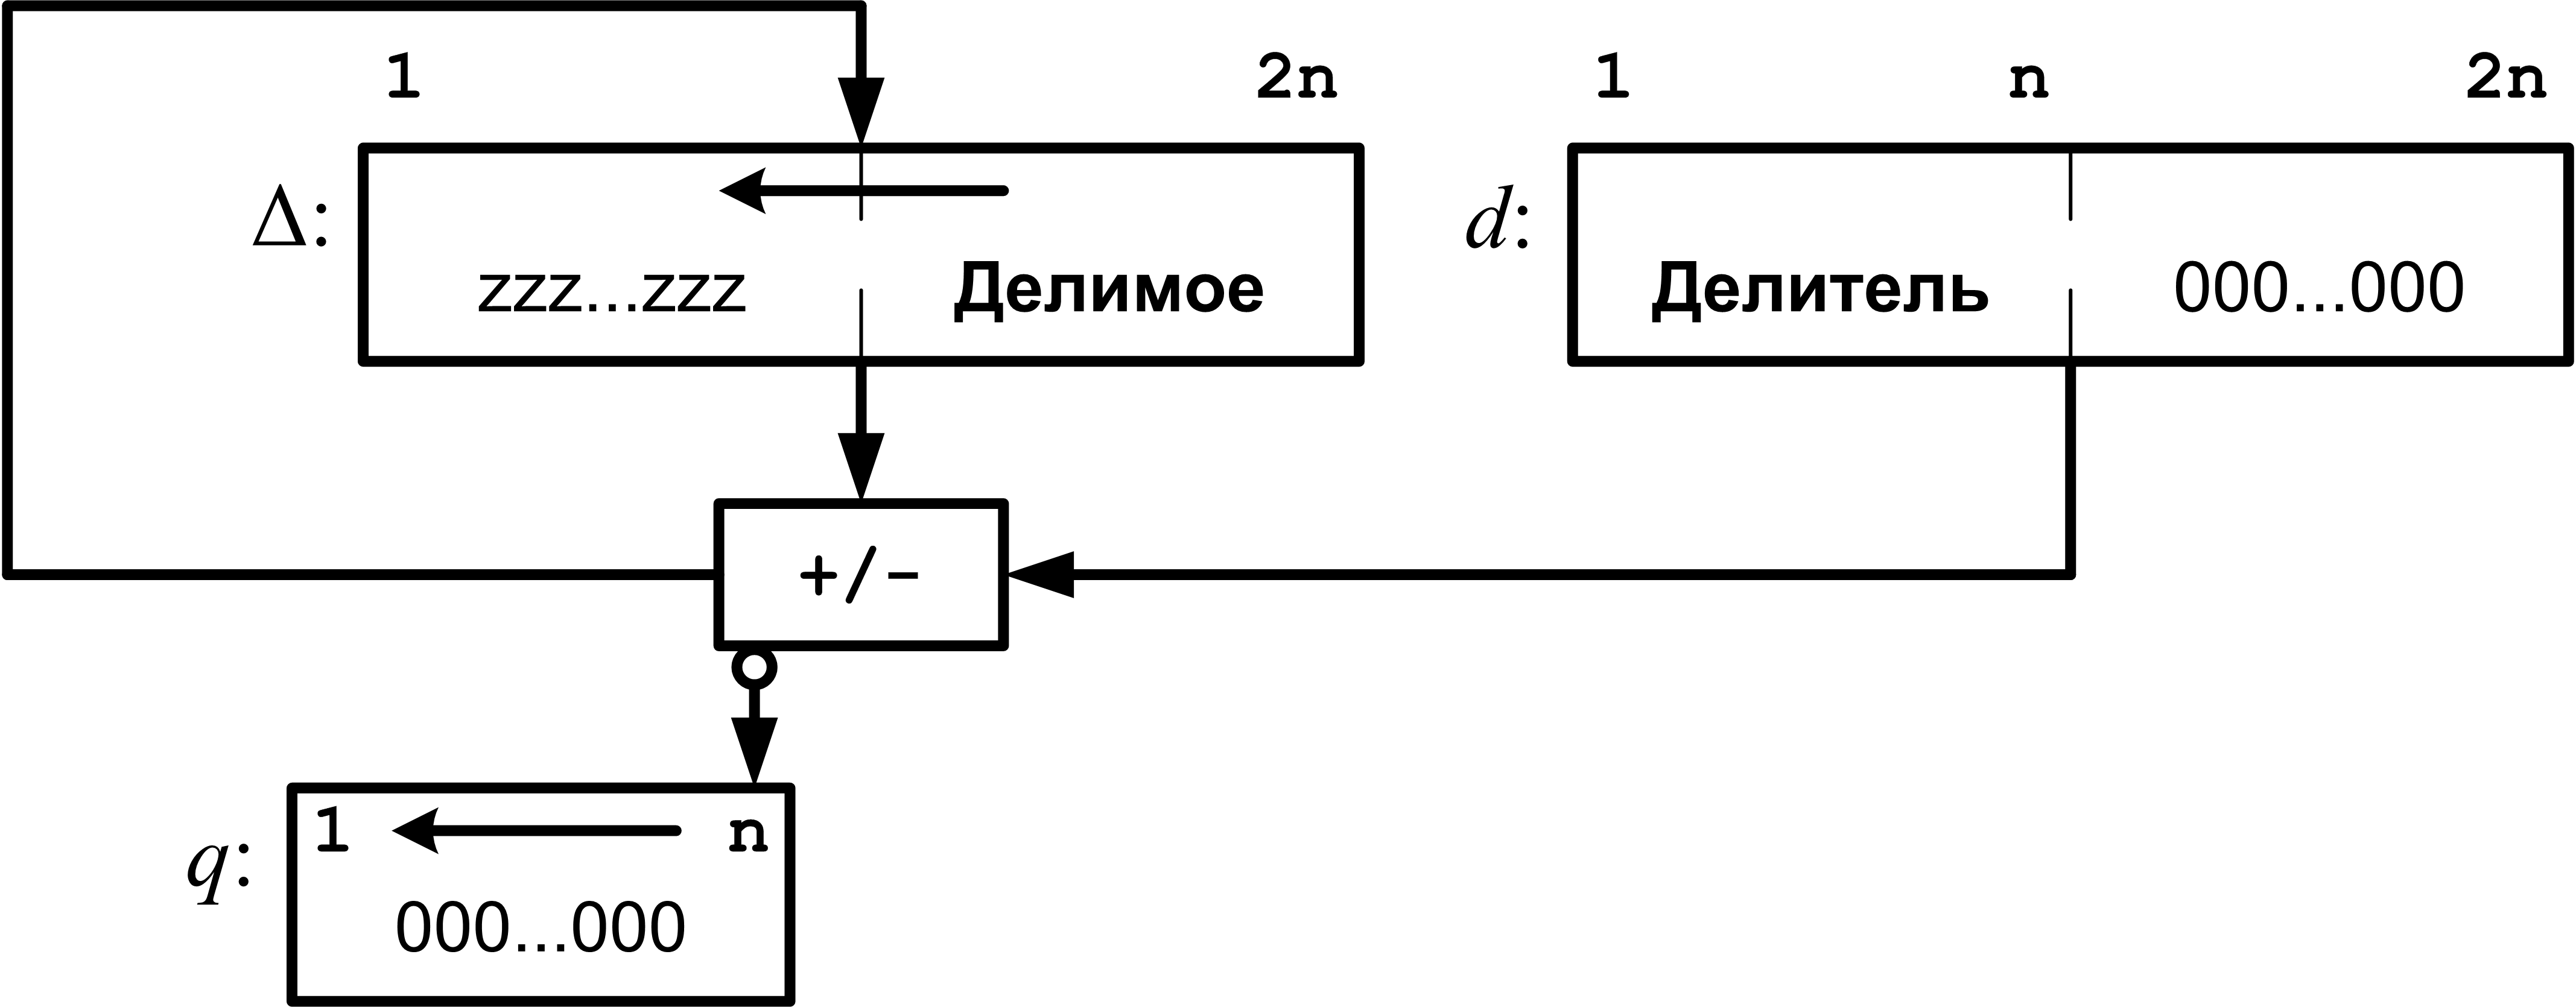
\includegraphics[width=0.47\textwidth]{fig/IDivBegin}
            & 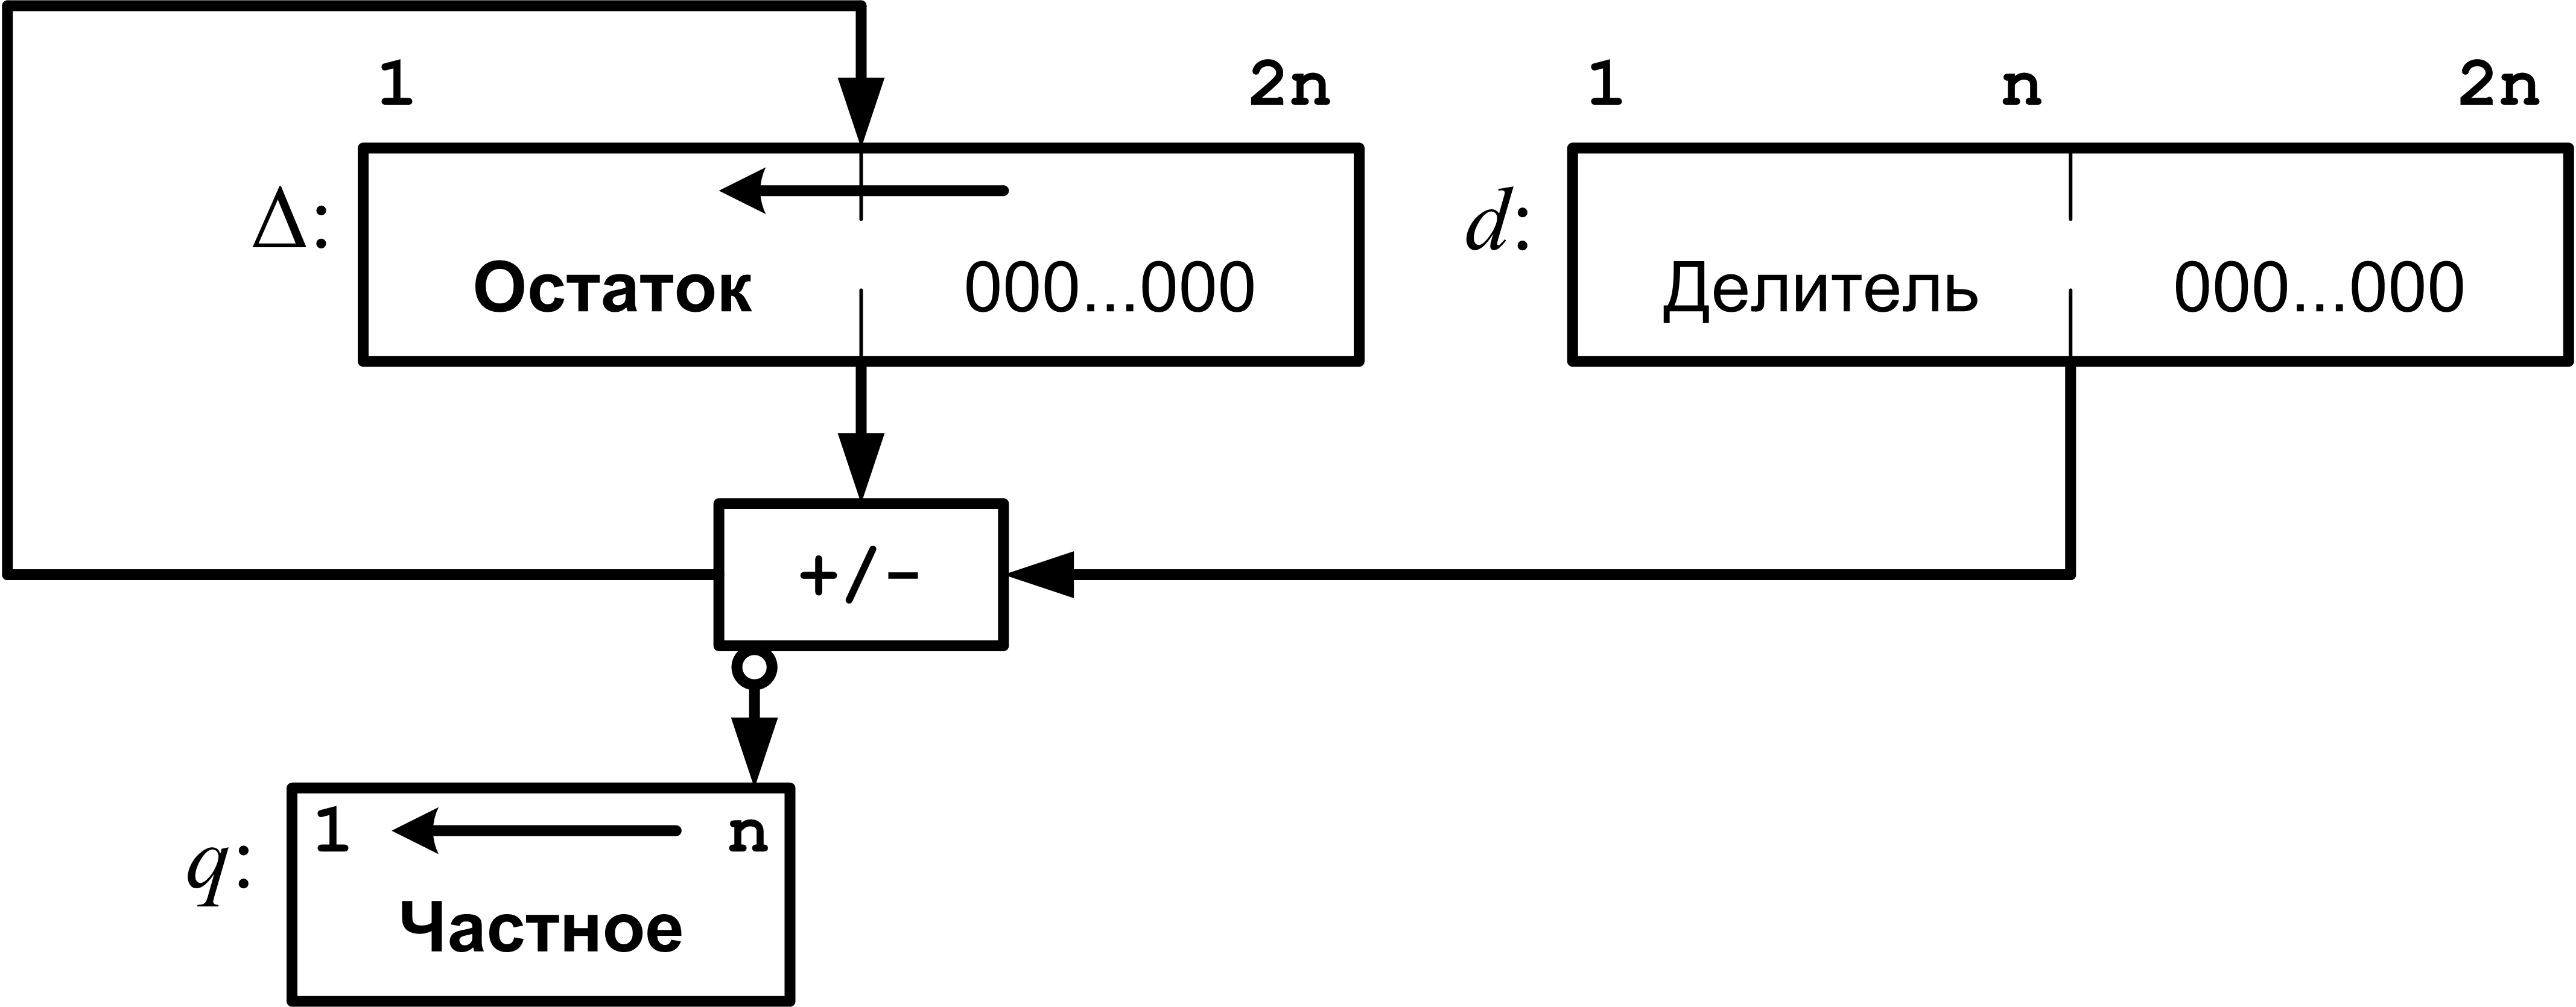
\includegraphics[width=0.47\textwidth]{fig/IDivEnd} \\
        а) начало деления
            & б) конец деления
    \end{tabular}
    \caption{I-й способ целочисленного деления} \label{t:div:int:Isp}
\end{figure}

\begin{figure}[!ht]
    \centering
    \begin{tabular}{c||c}
        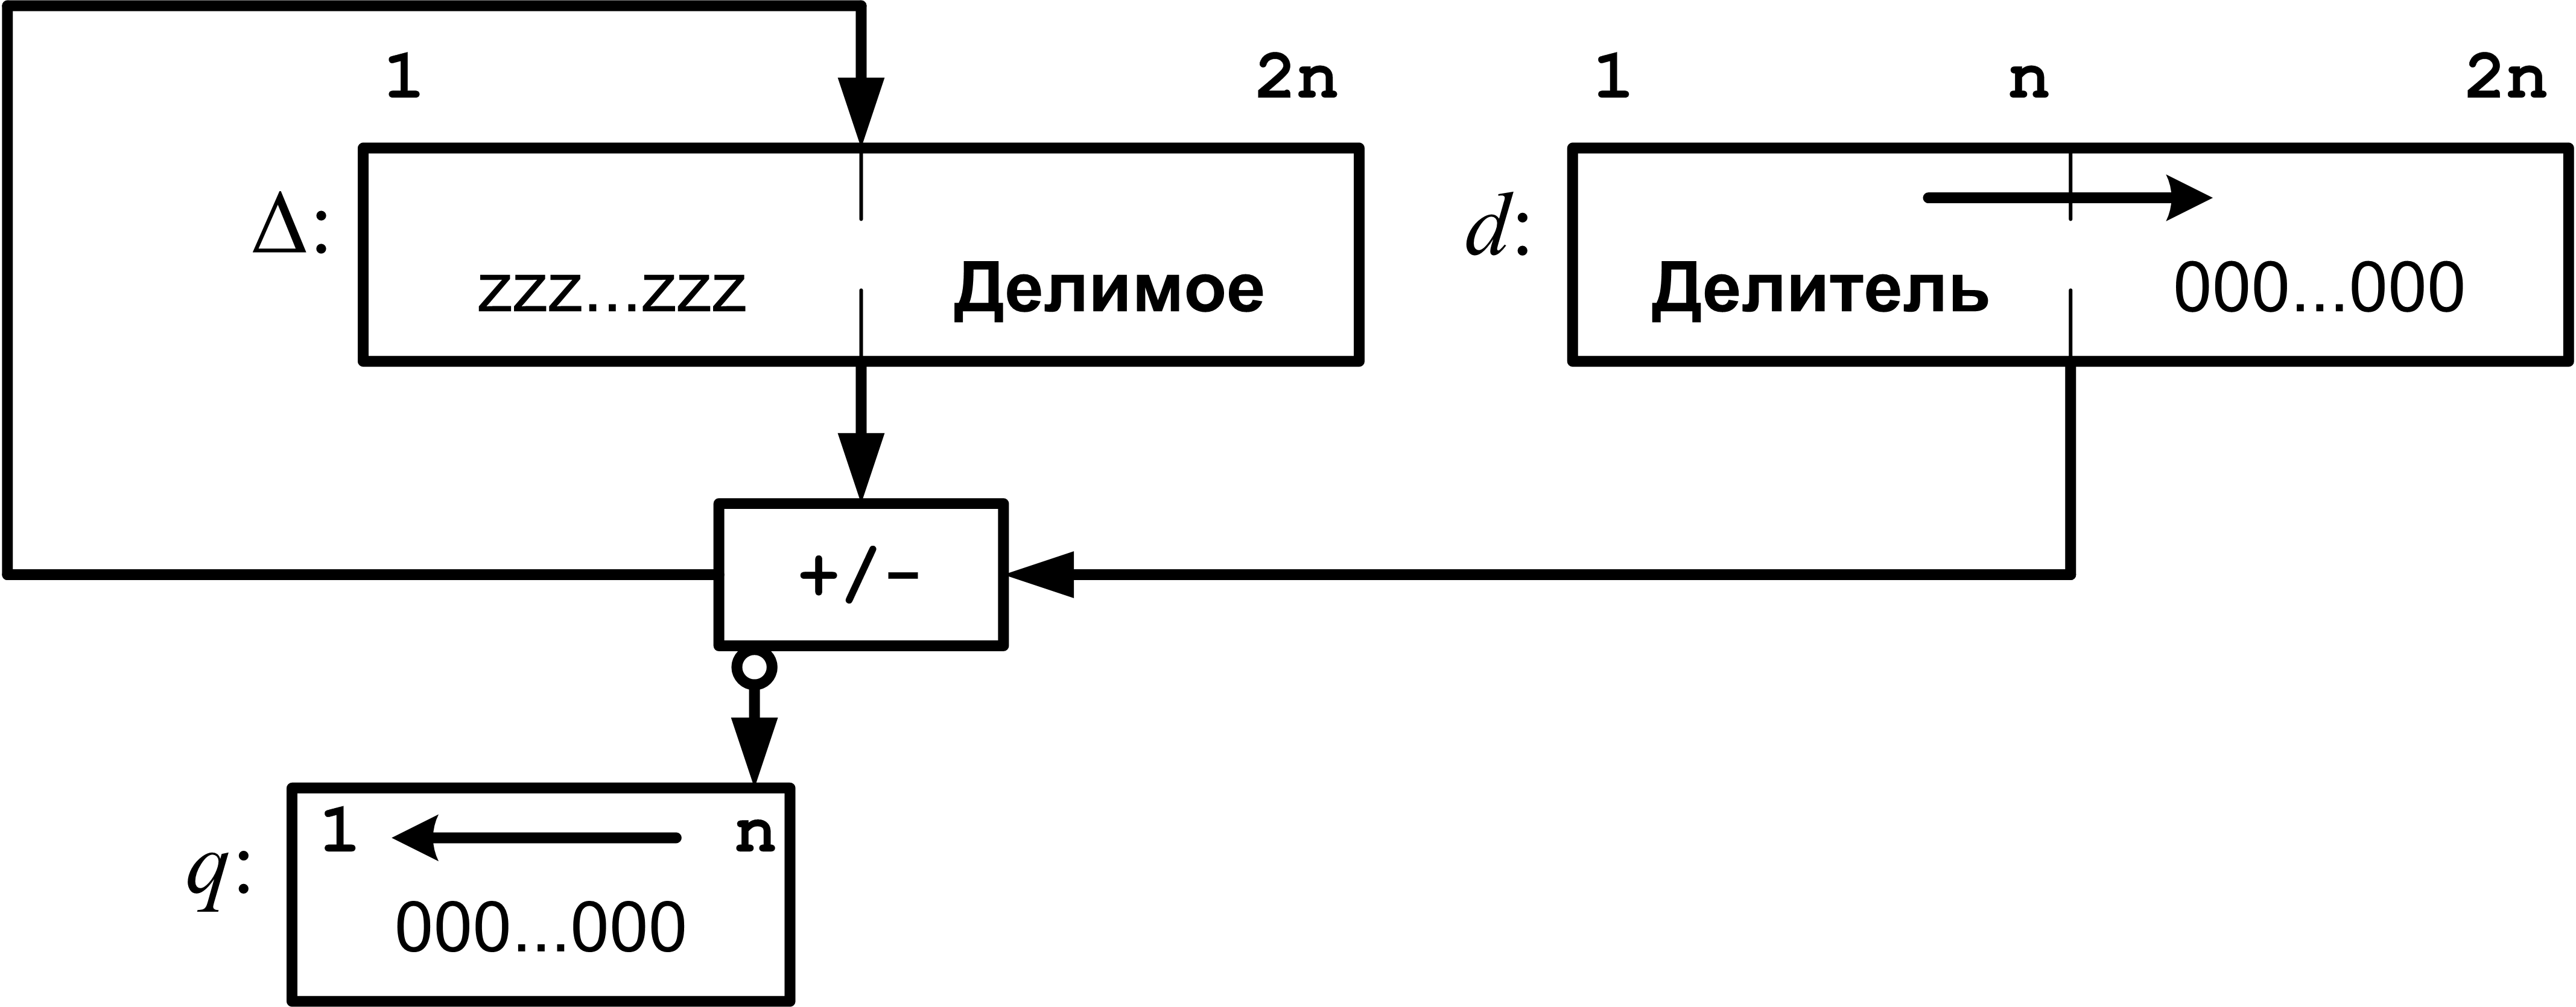
\includegraphics[width=0.47\textwidth]{fig/IIDivBegin}
            & 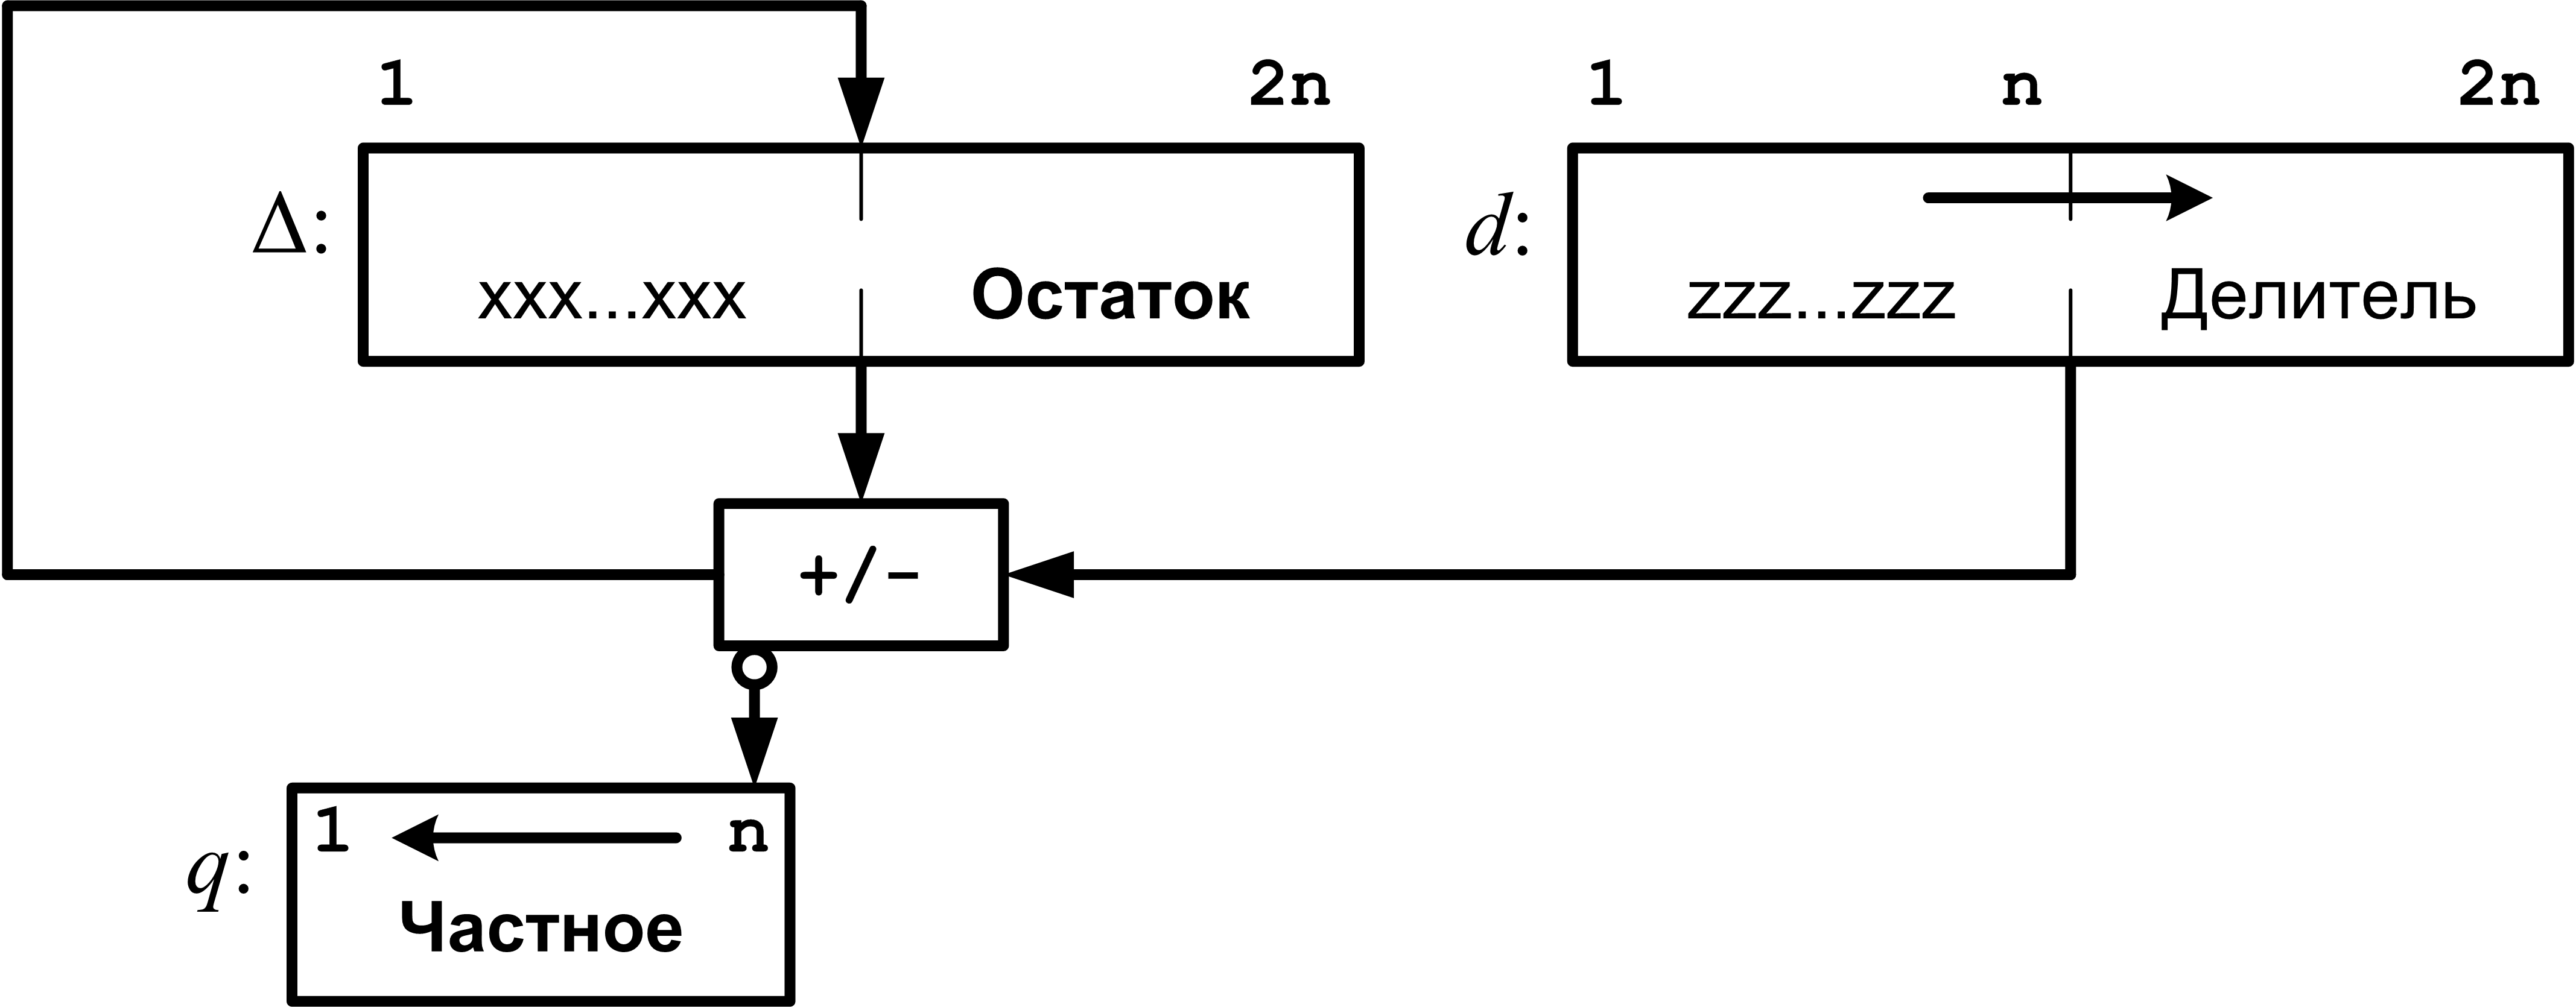
\includegraphics[width=0.47\textwidth]{fig/IIDivEnd} \\
        а) начало деления
            & б) конец деления
    \end{tabular}
    \caption{II-й способ целочисленного деления} \label{t:div:int:IIsp}
\end{figure}

Рассмотрим алгоритм деления с <<Восстановлением остатков>>. Особенностью данного алгоритма является то, что полученная разность регистров остатка $\Delta$ и делителя $d$ (остаток текущего шага) всегда запоминается в регистре остатков (что проще реализовать технически). И если в регистре остатка получено отрицательное значение, то требуется восстановить его положительное значение до вычитания, прибавив делитель.

Алгоритм деления с <<восстановлением остатков>> следующий.
\begin{enumerate}
	\item Если делитель --- ноль, то фиксируется ошибка вычислений и алгоритм завершается.
	\item $i\gets 1$. В младшую часть регистра остатков заносится делимое, в старшую часть регистра делителя --- делитель. Далее состояние регистра остатков --- остаток ($\Delta$), регистра делителя --- делитель ($d$), регистра частного ($q$) --- частное.
	\item\label{e:div:int:vo:start} Выполняются сдвиги: частное $q$ влево, остаток $\Delta$ влево (в первом способе), делитель $d$ вправо (во втором способе).
	\item Получается новый остаток $\Delta\gets(\Delta - d)$;
	\item Если $\Delta < 0$, то в младший разряд частного заносится $0$, иначе $1$.
	\item Если $\Delta < 0$, то выполняется \emph{восстановление} старого значения остатка: $\Delta\gets(\Delta + d)$.
	\item $i\gets (i + 1)$. Если $i\le n$, то к шагу \ref{e:div:int:vo:start}.
	\item В регистре частного получено значение частного, в регистре остатков --- $n$-разрядный остаток (в первом способе в старших разрядах, во втором --- в младших).
\end{enumerate}

Так как в основном цикле алгоритма происходит проверка знака остатка ($\Delta < 0$), то к регистру остатка и делителю добавляется знаковый разряд. Пример деления с восстановлением остатков I-м способом в шестиразрядной сетке приведен на рисунке \ref{t:div:int:IspVoEx}, а II-м --- на рисунке \ref{t:div:int:IIspVoEx}.

\begin{figure}[!ht]
    \centering
	\begin{tabular}{c|r|r|l}
		\hline\hline
		$q, \leftarrow$ 
			& \multicolumn{1}{|c|}{$\Delta, \leftarrow$}
				& \multicolumn{1}{|c|}{$d$}
					& прим.\\ 
		\hline\hline
		\Number{......}
			& \Number{.,...... 111001}
				& \Number{.,...110}
					& исх. операнды;\\ \hline\hline
		\Number{......}
			& \Number{.,.....1 11001.}
				& 
					& сдвиг;\\ \hline
		\Number{.....0}
			& \Addition{.,.....1 11001.}
					   {1,111010 ......}
					   {1,111011 11001.}
				& 
					& $\Delta_1<0$;\\ \hline
		\Number{.....0}
			& \Addition{1,111011 11001.}
					   {.,...110 ......}
					   {.,.....1 11001.}
				& 
					& ВО $\Delta_1$; \\ \hline
		\Number{....0.}
			& \Number{.,....11 1001..}
				& 
					& сдвиг;\\ \hline
		\Number{....00}
			& \Addition{.,....11 1001..}
					   {1,111010 ......}
					   {1,111101 1001..}
				& 
					& $\Delta_2<0$;\\ \hline
		\Number{....00}
			& \Addition{1,111101 1001..}
					   {.,...110 ......}
					   {.,....11 1001..}
				& 
					& ВО $\Delta_2$; \\ \hline
		\Number{...00.}
			& \Number{.,...111 001...}
				& 
					& сдвиг;\\ \hline
		\Number{...001}
			& \Addition{.,...111 001...}
					   {1,111010 ......}
					   {.,.....1 001...}
				& 
					& $\Delta_3> 0$; Без ВО\\ \hline
		\Number{..001.}
			& \Number{.,....10 01....}
				& 
					& сдвиг;\\ \hline
		\Number{..0010}
			& \Addition{.,....10 01....}
					   {1,111010 ......}
					   {1,111100 01....}
				& 
					& $\Delta_4<0$;\\ \hline
		\Number{..0010}
			& \Addition{1,111100 01....}
					   {.,...110 ......}
					   {.,....10 01....}
				& 
					& ВО $\Delta_4$; \\ \hline
		\Number{.0010.}
			& \Number{.,...100 1.....}
				& 
					& сдвиг;\\ \hline
		\Number{.00100}
			& \Addition{.,...100 1.....}
					   {1,111010 ......}
					   {1,111110 1.....}
				& 
					& $\Delta_5<0$;\\ \hline
		\Number{.00100}
			& \Addition{1,111110 1.....}
					   {.,...110 ......}
					   {.,...100 1.....}
				& 
					& ВО $\Delta_5$; \\ \hline
		\Number{00100.}
			& \Number{.,..1001 ......}
				& 
					& сдвиг;\\ \hline
		\Number{001001}
			& \Addition{.,..1001 ......}
					   {1,111010 ......}
					   {0,000011 ......}
				& 
					& $\Delta_6>0$; Без ВО\\ \hline\hline
		\Number{001001}
			& \Number{000011}
				&
					& $\DivAnswer{q}{\Delta_6}$;\\ 
	\end{tabular}
	
    \caption{$57\div 6 = \DivAnswer{9}{1}$ I-сп с восстановлением остатков, $n=6$}
    \label{t:div:int:IspVoEx}
\end{figure}

\begin{figure}[!ht]
    \centering
	\begin{tabular}{c|r|r|l}
		\hline\hline
		$q, \leftarrow$ 
			& \multicolumn{1}{|c|}{$\Delta$}
				& \multicolumn{1}{|c|}{$d,\rightarrow$}
					& прим. \\ 
		\hline\hline
		\Number{......}
			& \Number{.,...... 111110}
				& \Number{.,...110 ......}
					& операнды;\\ \hline\hline
		\Number{......}
			& 
				& \Number{.,....11 0.....}
					& сдвиг;\\ \hline
		\Number{.....0}
			& \Addition{.,...... 111110}
					   {1,111101 0.....}
					   {1,111101 111110}
				& 
					& $\Delta_1<0$;\\ \hline
		\Number{.....0}
			& \Addition{1,111101 111110}
					   {.,....11 0.....}
					   {.,...... 111110}
				& 
					& ВО $\Delta_1$;\\ \hline
		\Number{....0.}
			& 
				& \Number{.,.....1 10....}
					& сдвиг;\\ \hline
		\Number{....00}
			& \Addition{.,...... 111110}
					   {1,111110 10....}
					   {1,111111 011110}
				& 
					& $\Delta_2<0$;\\ \hline
		\Number{....00}
			& \Addition{1,111111 011110}
					   {.,.....1 10....}
					   {.,...... 111110}
				& 
					& ВО $\Delta_2$;\\ \hline
		\Number{...00.}
			& 
				& \Number{.,...... 110...}
					& сдвиг;\\ \hline
		\Number{...001}
			& \Addition{.,...... 111110}
					   {1,111111 010...}
					   {0,000000 001110}
				& 
					& $\Delta_3>0$; Без ВО\\ \hline
		\Number{..001.}
			& 
				& \Number{.,...... .110..}
					& сдвиг;\\ \hline
		\Number{..0010}
			& \Addition{.,...... ..1110}
					   {1,111111 1010..}
					   {1,111111 110110}
				& 
					& $\Delta_4<0$;\\ \hline
		\Number{..0010}
			& \Addition{1,111111 110110}
					   {.,...... .110..}
					   {.,...... ..1110}
				& 
					& ВО $\Delta_4$;\\ \hline
		\Number{.0010.}
			& 
				& \Number{.,...... ..110.}
					& сдвиг;\\ \hline
		\Number{.00101}
			& \Addition{.,...... ..1110}
					   {1,111111 11010.}
					   {0,000000 000010}
				& 
					& $\Delta_5>0$; Без ВО\\ \hline
		\Number{00101.}
			& 
				& \Number{.,...... ...110}
					& сдвиг;\\ \hline
		\Number{001010}
			& \Addition{.,...... ....10}
					   {1,111111 111010}
					   {1,111111 111100}
				& 
					& $\Delta_6<0$;\\ \hline
		\Number{001010}
			& \Addition{1,111111 111100}
					   {.,...... ...110}
					   {.,...... ....10}
				& 
					& ВО $\Delta_6$; \\ \hline\hline
	\Number{001010}
		& \Number{000010}
			&
				& $\DivAnswer{q}{\Delta_6}$;\\ 
	\end{tabular}
		
    \caption{$62\div 6 = \DivAnswer{10}{2}$ II-сп. с восстановлением остатков, $n=6$}
    \label{t:div:int:IIspVoEx}
\end{figure}

Рассмотрим, что произойдет с остатком в изложенном выше алгоритме деления с восстановлением остатков. 
Если новый остаток $\Delta$ получается отрицательным, то к нему прибавляется делитель, чтобы восстановить старое (положительное) значение остатка. Чтобы не тратить на это время (а на восстановление требуется такт) --- проследим, что происходит к моменту получения следующего остатка $\Delta'$.
    
\begin{itemize}
	\item В первом способе: 
	\[
		\Delta' = 
			\begin{cases}
				2\cdot\Delta + d, & \text{ если $\Delta<0$: $2\cdot(\underbrace{\Delta + d}_\text{В.О.}) - d = 2\cdot\Delta + d$,}\\
				2\cdot\Delta - d, & \text{ если $\Delta\ge 0$.}
			\end{cases}
	\]
	
	\item Во втором способе:
	\[
		\Delta' = 
			\begin{cases}
				\Delta + d/2, & \text{ если $\Delta<0$: $(\underbrace{\Delta + d}_\text{В.О.}) - d/2 = \Delta + d/2$,}\\
				\Delta - d/2, & \text{ если $\Delta\ge 0$.}
			\end{cases}
	\]
\end{itemize}

Таким образом, если остаток получается отрицательным, то восстановление не выполняется, а на следующем шаге после соответствующих сдвигов, делитель прибавляется к остатку.

Алгоритм деления без восстановления остатков.
\begin{enumerate}
	\item Если делитель --- ноль, то фиксируется ошибка вычислений и алгоритм завершается.
	\item $i\gets 1$; В младшую часть регистра остатков заносится делимое, в старшую часть регистра делителя --- делитель. Далее состояние регистра остатков --- остаток ($\Delta$), регистра делителя --- делитель ($d$), регистра частного ($q$) --- частное.
	\item\label{div:wvo:start} Выполняются сдвиги: частное $q$ влево, остаток $\Delta$ влево (в первом способе), делитель $d$ вправо (во втором способе).
	\item Если $\Delta < 0$, то $\Delta\gets(\Delta + d)$, иначе $\Delta\gets(\Delta - d)$;
	\item Если $\Delta < 0$, то в младший разряд частного заносится 0, иначе 1.
	\item $i\gets (i + 1)$. Если $\le n$, то к шагу \ref{div:wvo:start}.
	\item Восстанавливается последний остаток. Если $\Delta < 0$, то $\Delta\gets(\Delta + d)$.
	\item В регистре частного получено значение частного, в регистре остатков --- $n$-разрядный остаток (в первом способе в старших разрядах, во втором --- в младших).
\end{enumerate}


На рисунках \ref{t:div:int:IspNoVoEx} и \ref{t:div:int:IIspNoVoEx} приводятся примеры деления без восстановления остатков I и II-м способами соответственно. Сравните результаты с примерами на рисунках \ref{t:div:int:IspVoEx} и \ref{t:div:int:IIspVoEx}.

\begin{figure}[!ht]
    \centering
	\begin{tabular}{c|r|r|l}
		\hline\hline
		$q, \leftarrow$ 
			& \multicolumn{1}{|c|}{$\Delta, \leftarrow$}
				& \multicolumn{1}{|c|}{$d$}
					& прим.\\ 
		\hline\hline
		\Number{......}
			& \Number{.,...... 111001}
				& \Number{.,...110}
					& исх. операнды;\\ \hline\hline
		\Number{......}
			& \Number{.,.....1 11001.}
				& 
					& сдвиг;\\ \hline
		\Number{.....0}
			& \Addition{.,.....1 11001.}
					   {1,111010 ......}
					   {1,111011 11001.}
				& 
					& ${-d},\Delta_1<0$;\\ \hline
		\Number{....0.}
			& \Number{1,110111 1001..}
				& 
					& сдвиг;\\ \hline
		\Number{....00}
			& \Addition{1,110111 1001..}
					   {.,...110 ......}
					   {1,111101 1001..}
				& 
					& ${+d},\Delta_2<0$;\\ \hline
		\Number{...00.}
			& \Number{1,111011 001...}
				& 
					& сдвиг;\\ \hline
		\Number{...001}
			& \Addition{1,111011 001...}
					   {.,...110 ......}
					   {.,.....1 001...}
				& 
					& $\Delta_3> 0$;\\ \hline
		\Number{..001.}
			& \Number{.,....10 01....}
				& 
					& сдвиг;\\ \hline
		\Number{..0010}
			& \Addition{.,....10 01....}
					   {1,111010 ......}
					   {1,111100 01....}
				& 
					& ${-d},\Delta_4<0$;\\ \hline
		\Number{.0010.}
			& \Number{1,111000 1.....}
				& 
					& сдвиг;\\ \hline
		\Number{.00100}
			& \Addition{1,111000 1.....}
					   {.,...110 ......}
					   {1,111110 1.....}
				& 
					& $\Delta_5<0$;\\ \hline
		\Number{00100.}
			& \Number{1,111101 ......}
				& 
					& сдвиг;\\ \hline
		\Number{001001}
			& \Addition{1,111101 ......}
					   {.,...110 ......}
					   {0,000011 ......}
				& 
					& $\Delta_6>0$;\\ \hline\hline
		\Number{001001}
			& \Number{000011}
				&
					& $\DivAnswer{q}{\Delta_6}$;\\ 
	\end{tabular}
	
    \caption{$57\div 6 = \DivAnswer{9}{1}$ I-сп без восстановления остатков, $n=6$}
    \label{t:div:int:IspNoVoEx}
\end{figure}

\begin{figure}[!ht]
    \centering
	\begin{tabular}{c|r|r|l}
		\hline\hline
		$q, \leftarrow$ 
			& \multicolumn{1}{|c|}{$\Delta$}
				& \multicolumn{1}{|c|}{$d,\rightarrow$}
					& прим. \\ 
		\hline\hline
		\Number{......}
			& \Number{.,...... 111110}
				& \Number{.,...110 ......}
					& операнды;\\ \hline\hline
		\Number{......}
			& \Number{.,...... 111110}
				& \Number{.,....11 0.....}
					& сдвиг;\\ \hline
		\Number{.....0}
			& \Addition{.,...... 111110}
					   {1,111101 0.....}
					   {1,111101 111110}
				& 
					& $-d, \Delta_1<0$;\\ \hline
		\Number{....0.}
			& 
				& \Number{.,.....1 10....}
					& сдвиг;\\ \hline
		\Number{....00}
			& \Addition{1,111101 111110}
					   {.,.....1 10....}
					   {1,111111 011110}
				& 
					& $+d, \Delta_2<0$;\\ \hline
		\Number{...00.}
			& 
				& \Number{.,...... 110...}
					& сдвиг;\\ \hline
		\Number{...001}
			& \Addition{1,111111 011110}
					   {.,...... 110...}
					   {.,...... ..1110}
				& 
					& $+d, \Delta_3>0$;\\ \hline
		\Number{..001.}
			& 
				& \Number{.,...... .110..}
					& сдвиг;\\ \hline
		\Number{..0010}
			& \Addition{.,...... ..1110}
					   {1,111111 1010..}
					   {1,111111 110110}
				& 
					& $-d, \Delta_4<0$;\\ \hline
		\Number{.0010.}
			& 
				& \Number{.,...... ..110.}
					& сдвиг;\\ \hline
		\Number{.00101}
			& \Addition{1,111111 110110}
					   {.,...... ..110.}
					   {.,...... ....10}
				& 
					& $+d, \Delta_5>0$;\\ \hline
		\Number{00101.}
			& 
				& \Number{.,...... ...110}
					& сдвиг;\\ \hline
		\Number{001010}
			& \Addition{.,...... ....10}
					   {1,111111 111010}
					   {1,111111 111100}
				& 
					& $-d, \Delta_6<0$;\\ \hline
		\Number{001010}
			& \Addition{1,111111 111100}
					   {.,...... ...110}
					   {.,...... ....10}
				& 
					& ВО!!! $\Delta_6$; \\ \hline\hline
	\Number{001010}
		& \Number{000010}
			&
				& $\DivAnswer{q}{\Delta_6}$;\\ 
	\end{tabular}
		
    \caption{$62\div 6 = \DivAnswer{10}{2}$ II-сп. с восстановлением остатков, $n=6$}
    \label{t:div:int:IIspNoVoEx}
\end{figure}


\subsection{Деление чисел в дополнительном коде}

Пусть $S(x)$ --- функция, возвращающая знак целого числа $x$. При делении чисел со знаком определение очередного разряда частного будет выполняться по следующим правилам.
\begin{enumerate}
	\item\label{en:div:int:rule:mod} Если знаки делимого $A$ и текущего остатка $\Delta$ совпадают ($S(A)=S(\Delta)$), то разряд частного (модуля) $q_0\gets 1$, иначе $q_0\gets 0$. Таким образом находятся, очевидно, разряды модуля частного.
	\item\label{en:div:int:rule:neg} Далее, если $S(A)$ и $S(d)$ различны, то полученный разряд частного следует инвертировать: $q_0\gets(\lnot q_0)$. Так учитывается, что частное должно получиться отрицательным. Строго говоря, так будут получены разряды обратного кода частного.
\end{enumerate}
    
Так как справедливо, что
\[
	(a=b)\Leftrightarrow \lnot(a\oplus b) \Leftrightarrow (1\oplus a\oplus b),
\]
то исходное правило, записанное одной формулой
\[
	q_0\gets\underbrace{
		\underbrace{\lnot(S(A)=S(\Delta))}_{\text{п. \ref{en:div:int:rule:mod}}}\oplus(S(A)\oplus S(d))
	}_{\text{п. \ref{en:div:int:rule:neg}}}
\]
можно значительно упростить:
\begin{align*}
	\lnot(S(A)=S(\Delta))\oplus(S(A)\oplus S(d)) \Leftrightarrow \\
	\Leftrightarrow(1\oplus S(A)\oplus S(\Delta))\oplus (S(A)\oplus S(d)) \Leftrightarrow (1\oplus S(d)\oplus S(\Delta))\Leftrightarrow \\
	\Leftrightarrow\lnot(S(d)\oplus S(\Delta)).
\end{align*}

Алгоритм деления в ДК без восстановления остатков.
\begin{enumerate}
	\item Если делтель --- ноль, то фиксируется ошибка вычислений и алгоритм завершается.
	\item $i\gets 1$. Инициализируются регистры $q$, $\Delta$ и $d$.
	\item\label{div:dcvo:start} Выполняются сдвиги: $q$ --- влево, $\Delta$ --- влево (I сп.), $d$ --- вправо (II~сп., с учётом знака).
	\item Если знаки $\Delta$ и $d$ совпадают, то $\Delta\gets(\Delta - d)$, иначе $\Delta\gets(\Delta + d)$.
	\item $q_0\gets\lnot(S(d)\oplus S(\Delta))$. Т.е. если знаки $d$ и $\Delta$ совпадают, то $q_0\gets 1$, иначе $q_0\gets 0$.
	\item $i\gets (i + 1)$. Если $i<=n$, то к шагу \ref{div:dcvo:start}.
	\item Выполняется процедура коррекции остатка и частного, действия которой в зависимости от знаков делимого и делителя приведены на рисунке \ref{t:div:int:Signed:Correction}.
\end{enumerate}

\begin{figure}[!ht]
    \centering
	\begin{tabular}{c||c|c}
			& $d> 0$
				& $d < 0$\\
		\hline\hline
		\rotatebox{90}{$A\ge 0$}
			& 
			\parbox[c]{.3\textwidth}{
				\begin{align*}
					q&\gets q,\\
					\Delta&\gets 
					\begin{cases}
						(\Delta + d), & \Delta < 0, \\
						\Delta,      &\text{ иначе,}
					\end{cases}
				\end{align*}
			}
				& 
				\parbox[c]{.3\textwidth}{
					\begin{align*}
						q&\gets (q+1),\\
						\Delta&\gets 
						\begin{cases}
							(\Delta - d), & \Delta < 0, \\
							\Delta,       &\text{ иначе,}
						\end{cases}
					\end{align*}
				}
				\\
		\hline
		\rotatebox{90}{$A < 0$}
			& 
			\parbox[c]{.3\textwidth}{
				\begin{align*}
					q&\gets 
					\begin{cases}
						q,      & (\Delta = 0) \lor (\Delta = -d) \\
						(q+1),  &\text{ иначе,}
					\end{cases}
					\\
					\Delta&\gets 
					\begin{cases}
						0,          & (\Delta = 0) \lor (\Delta = -d), \\
						(\Delta-d), & \Delta > 0, \\
						\Delta,     & \text{ иначе,}
					\end{cases}
				\end{align*}
			}
				& 
				\parbox[c]{.3\textwidth}{
					\begin{align*}
						q&\gets 
						\begin{cases}
							q+1, & (\Delta = 0) \lor (\Delta = d), \\
							q,   &\text{ иначе,}
						\end{cases}
						\\
						\Delta&\gets 
						\begin{cases}
							0,        & (\Delta = 0) \lor (\Delta = d), \\
							\Delta+d, & \Delta > 0, \\
							\Delta,   & \text{ иначе.}
						\end{cases}
					\end{align*}
				} \\ 
	\end{tabular}
	
    \caption{Правила заключительной коррекции остатка и частного по правилу отсечения в алгоритме знакового деления}
    \label{t:div:int:Signed:Correction}
\end{figure}

Пример деления чисел со знаком первым способом приведен на рисунке \ref{t:div:int:Signed:I}.

\begin{figure}[!ht]
    \centering
	\begin{tabular}{c|r|r|l}
		\hline\hline
		$q, \leftarrow$ 
			& \multicolumn{1}{|c|}{$\Delta, \leftarrow$}
				& \multicolumn{1}{|c|}{$d$}
					& прим. \\ 
		\hline\hline
		\Number{......}
			& \Number{0,...... 011100}
				& \Number{1,111011}
					& операнды;\\ \hline\hline
		\Number{......}
			& \Number{0,.....0 11100.}
				& 
					& сдвиг;\\ \hline
		\Number{.....1}
			& \Addition{0,.....0 11100.}
					   {1,111011 ......}
					   {1,111011 11100.}
				& 
					& $+d, \Delta_1<0$;\\ \hline
		\Number{....1.}
			& \Number{1,110111 1100..}
				& 
					& сдвиг;\\ \hline
		\Number{....11}
			& \Addition{1,110111 1100..}
					   {.,...101 ......}
					   {1,111100 1100..}
				& 
					& $-d,\Delta_2<0$;\\ \hline
		\Number{...11.}
			& \Number{1,111001 100...}
				& 
					& сдвиг;\\ \hline
		\Number{...111}
			& \Addition{1,111001 100...}
					   {.,...101 ......}
					   {1,111110 100...}
				& 
					& $-d,\Delta_3<0$;\\ \hline
		\Number{..111.}
			& \Number{1,111101 00....}
				& 
					& сдвиг;\\ \hline
		\Number{..1110}
			& \Addition{1,111101 00....}
					   {.,...101 ......}
					   {0,000010 00....}
				& 
					& $-d,\Delta_4>0$;\\ \hline
		\Number{.1110.}
			& \Number{0,000100 0.....}
				& 
					& сдвиг;\\ \hline
		\Number{.11101}
			& \Addition{0,000100 0.....}
					   {1,111011 ......}
					   {1,111111 0.....}
				& 
					& $+d,\Delta_5<0$;\\ \hline
		\Number{11101.}
			& \Number{1,111110 ......}
				& 
					& сдвиг;\\ \hline
		\Number{111010}
			& \Addition{1,111110 ......}
					   {0,000101 ......}
					   {0,000011 ......}
				& 
					& $-d,\Delta_6>0$;\\ \hline\hline
		\Number{111011}
			& \Number{0,000011 ......}
				& 
					& $q\gets(q+1)$;\\ \hline
		\Number{111011}
			& \Number{000011}
				& 
					& Рез-т;\\
	\end{tabular}

    \caption{$28\div{-5} = \DivAnswer{-5}{3}$ I-сп без ВО, $n=6$}
    \label{t:div:int:Signed:I}
\end{figure}
 %целочисленное деление
\section{Деление в формате с плавающей точкой}
\label{ch:div:fpt}

Пусть $A$ --- делимое, $d$ --- делитель. В формате с плавающей запятой эти числа будут представлены так:
\[
    A=\FloatExpression{A}{2}, d=\FloatExpression{d}{2}.
\]

Результатом деления на ненулевой делитель будет частное $q=\FloatExpression{q}{2}$:

\[
    q=\frac{A}{d}=
    \frac{\FloatExpression{A}{2}}{\FloatExpression{d}{2}}=\left(\frac{\MantissOf{A}}{\MantissOf{d}}\right)\cdot 2^{(\OrderOf{A}-\OrderOf{d})},
\]
мантисса и порядок которого будут:
\[
    \MantissOf{q} = \frac{\MantissOf{A}}{\MantissOf{d}}, \OrderOf{q}=(\OrderOf{A}-\OrderOf{d}).
\]

Мантисса частного $\MantissOf{q}$, как результат деления мантисс операндов, может оказаться ненормализованной, и в этом случае требуется её нормализовать и скорректировать порядок $\OrderOf{q}$.

\paragraph{Базовый алгоритм деления ненулевых чисел $\frac{A}{d}$.}
\begin{enumerate}
    \item Вычитанием из порядка делимого порядка делителя определяется порядок частного: $\OrderOf{q}=(\OrderOf{A}-\OrderOf{d})$. Уже на этом шаге можно выявить ошибки переполнения разрядной сетки (ПРС) или потери младших разрядов (ПМР) и завершить выполнение операции.
    \item Делением мантиссы делимого на мантиссу делителя определяется мантисса частного: $\MantissOf{q}=\frac{\MantissOf{A}}{\MantissOf{d}}$. Деление мантисс обсуждается в разделе \ref{ch:div:fpt:divmant}.
    \item Если необходимо, выполняется нормализация частного $q$. Фиксируется результат или ошибка.
\end{enumerate}

Результат деления чисел в формате с плавающей точкой редко получается точным. Как известно из обсуждения формата в главе \ref{ch:digitFormat}, абслютная погрешность представления зависит от порядка (и порой может достигать огромных величин), а относительная погрешность не превышает $\frac{100}{2^{n}}\%$, где $n$ --- разрядность двоичной мантиссы.


\subsection{Особенности деления мантисс}
\label{ch:div:fpt:divmant}

Рассмотрим пример деления двух мантисс (нормализованных дробных чисел) в десятичной системе счисления:
\[0.31136/0.25714 \approx 1.21085.\]

Как и в целочисленном делении (см. раздел \ref{ch:div:int}), цифры частного будем записывать над соответствующими разрядами делимого.

На первом шаге определяется единственная цифра целой части:
\[
    \begin{tabular}{ccccccccccc|cl}
          & 1 &,  &   &   &   &   &   &   &   &   &                     & Примечания\\ 
          \hline\hline
          & 0 &.3 & 1 & 1 & 3 & 6 &   &   &   &   & ${\div 0.25714}$    &\\
          \hline\hline
          &   &,3 & 1 & 1 & 3 & 6 &   &   &   &   &                     &\\
        - &   &,2 & 5 & 7 & 1 & 4 &   &   &   &   &                     &$=0.25714\times 1$\\
        = &   &,0 & 5 & 4 & 2 & 2 &   &   &   &   &                     &\\ \hline
    \end{tabular}
\]

На втором шаге --- первая цифра дробной части:
\[
    \begin{tabular}{ccccccccccc|cl}
          & 1 &,2 &   &   &   &   &   &   &   &   &                     & Примечания\\ 
          \hline\hline
          & 0 &.3 & 1 & 1 & 3 & 6 &   &   &   &   & ${\div 0.25714}$    &\\
          \hline\hline
          &   &,3 & 1 & 1 & 3 & 6 &   &   &   &   &                     &\\
        - &   &,2 & 5 & 7 & 1 & 4 &   &   &   &   &                     &$=0.25714\times 1$\\
        = &   &,0 & 5 & 4 & 2 & 2 &   &   &   &   &                     &\\ \hline
          &   &   &,5 & 4 & 2 & 2 &   &   &   &   &                     &\\ 
        - &   &   &,5 & 1 & 4 & 2 & 8 &   &   &   &                     &$=0.25714\times 2$\\
        = &   &   &,0 & 2 & 7 & 9 & 2 &   &   &   &                     &\\ \hline
    \end{tabular}
\]

Процесс продолжается до тех пор, пока не будет определено достаточное количество цифр результата. Все шаги процесса деления приведены на рисунке \ref{t:div:fpt:decimalDiv}.

\begin{figure}[!ht]
    \centering
    \begin{tabular}{ccccccccccc|cl}
           
          & 1 &,2 & 1 & 0 & 8 & 5 &   &   &   &   &                     & Примечания\\ 
          \hline\hline
          & 0 &.3 & 1 & 1 & 3 & 6 &   &   &   &   & ${\div 0.25714}$    &\\
          \hline\hline
          &   &,3 & 1 & 1 & 3 & 6 &   &   &   &   &                     &\\
        - &   &,2 & 5 & 7 & 1 & 4 &   &   &   &   &                     &$=0.25714\times 1$\\
        = &   &,0 & 5 & 4 & 2 & 2 &   &   &   &   &                     &\\ \hline
          &   &   &,5 & 4 & 2 & 2 &   &   &   &   &                     &\\ 
        - &   &   &,5 & 1 & 4 & 2 & 8 &   &   &   &                     &$=0.25714\times 2$\\
        = &   &   &,0 & 2 & 7 & 9 & 2 &   &   &   &                     &\\ \hline
          &   &   &   &,2 & 7 & 9 & 2 &   &   &   &                     &\\ 
        - &   &   &   &,2 & 5 & 7 & 1 & 4 &   &   &                     &$=0.25714\times 1$\\
        = &   &   &   &,0 & 2 & 2 & 0 & 6 &   &   &                     &\\ \hline
          &   &   &   &   &,2 & 2 & 0 & 6 &   &   &                     &\\ 
        - &   &   &   &   &,0 & 0 & 0 & 0 &   &   &                     &$=0.25714\times 0$\\
        = &   &   &   &   &,2 & 2 & 0 & 6 &   &   &                     &\\ \hline
          &   &   &   &   & 2 &,2 & 0 & 6 &   &   &                     &\\ 
        - &   &   &   &   & 2 &,0 & 5 & 7 & 1 & 2 &                     &$=0.25714\times 8$\\
        = &   &   &   &   & 0 &,1 & 4 & 8 & 8 & 8 &                     &\\ \hline
          &   &   &   &   &   & 1 &,4 & 8 & 8 & 8 &                     &\\ 
        - &   &   &   &   &   & 1 &,2 & 8 & 5 & 7 &                     &$=0.25714\times 5$\\
        = &   &   &   &   &   & 0 &,2 & 0 & 3 & 1 &                     &\\ \hline
    \end{tabular}
	
    \caption{$0.31136/0.25714 \approx 1.21085$ в 10СС}
    \label{t:div:fpt:decimalDiv}
\end{figure}

Схемы делительных устройств для мантисс незначительно отличаются от схемам целочисленного деления (см. рисунки \ref{t:div:int:Isp}, \ref{t:div:int:IIsp}). Схема первого способа деления мантисс приведена на рисунке \ref{t:div:fpt:Isp}, а схема второго --- на рисунке \ref{t:div:fpt:IIsp}.

\begin{figure}[!ht]
    \centering
    \begin{tabular}{c||c}
        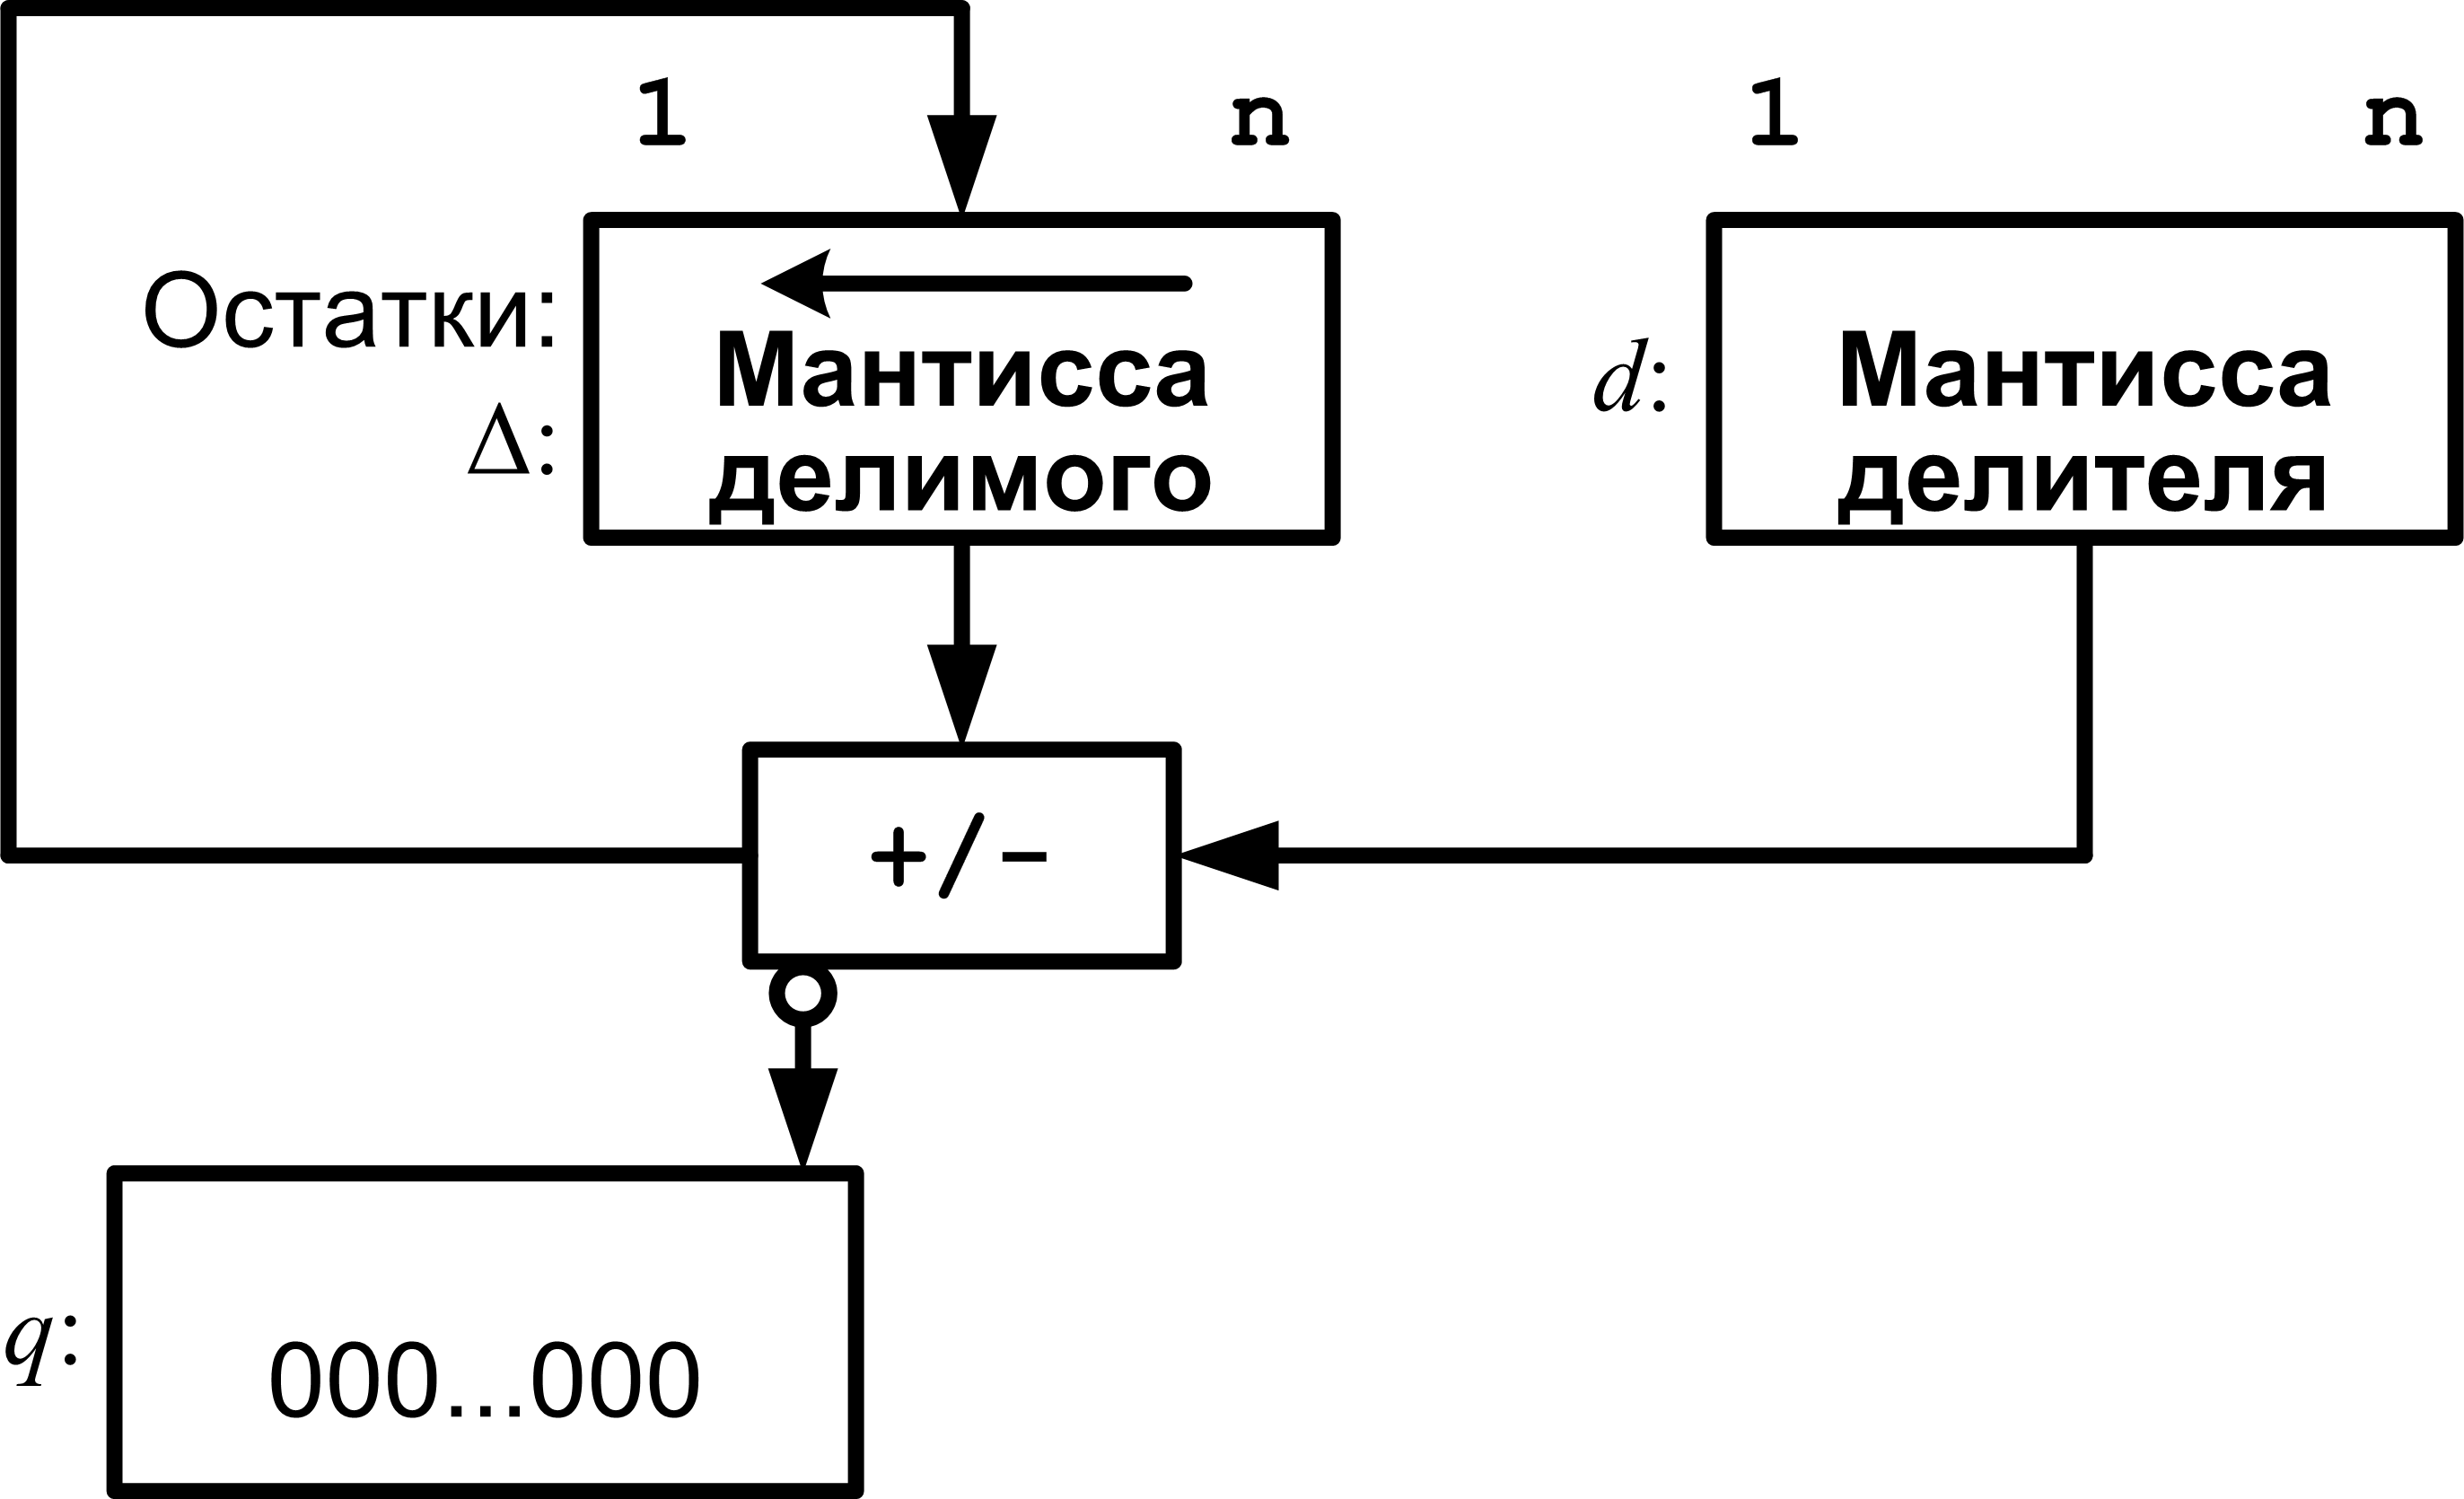
\includegraphics[width=0.47\textwidth]{fig/IFDivBegin}
            & 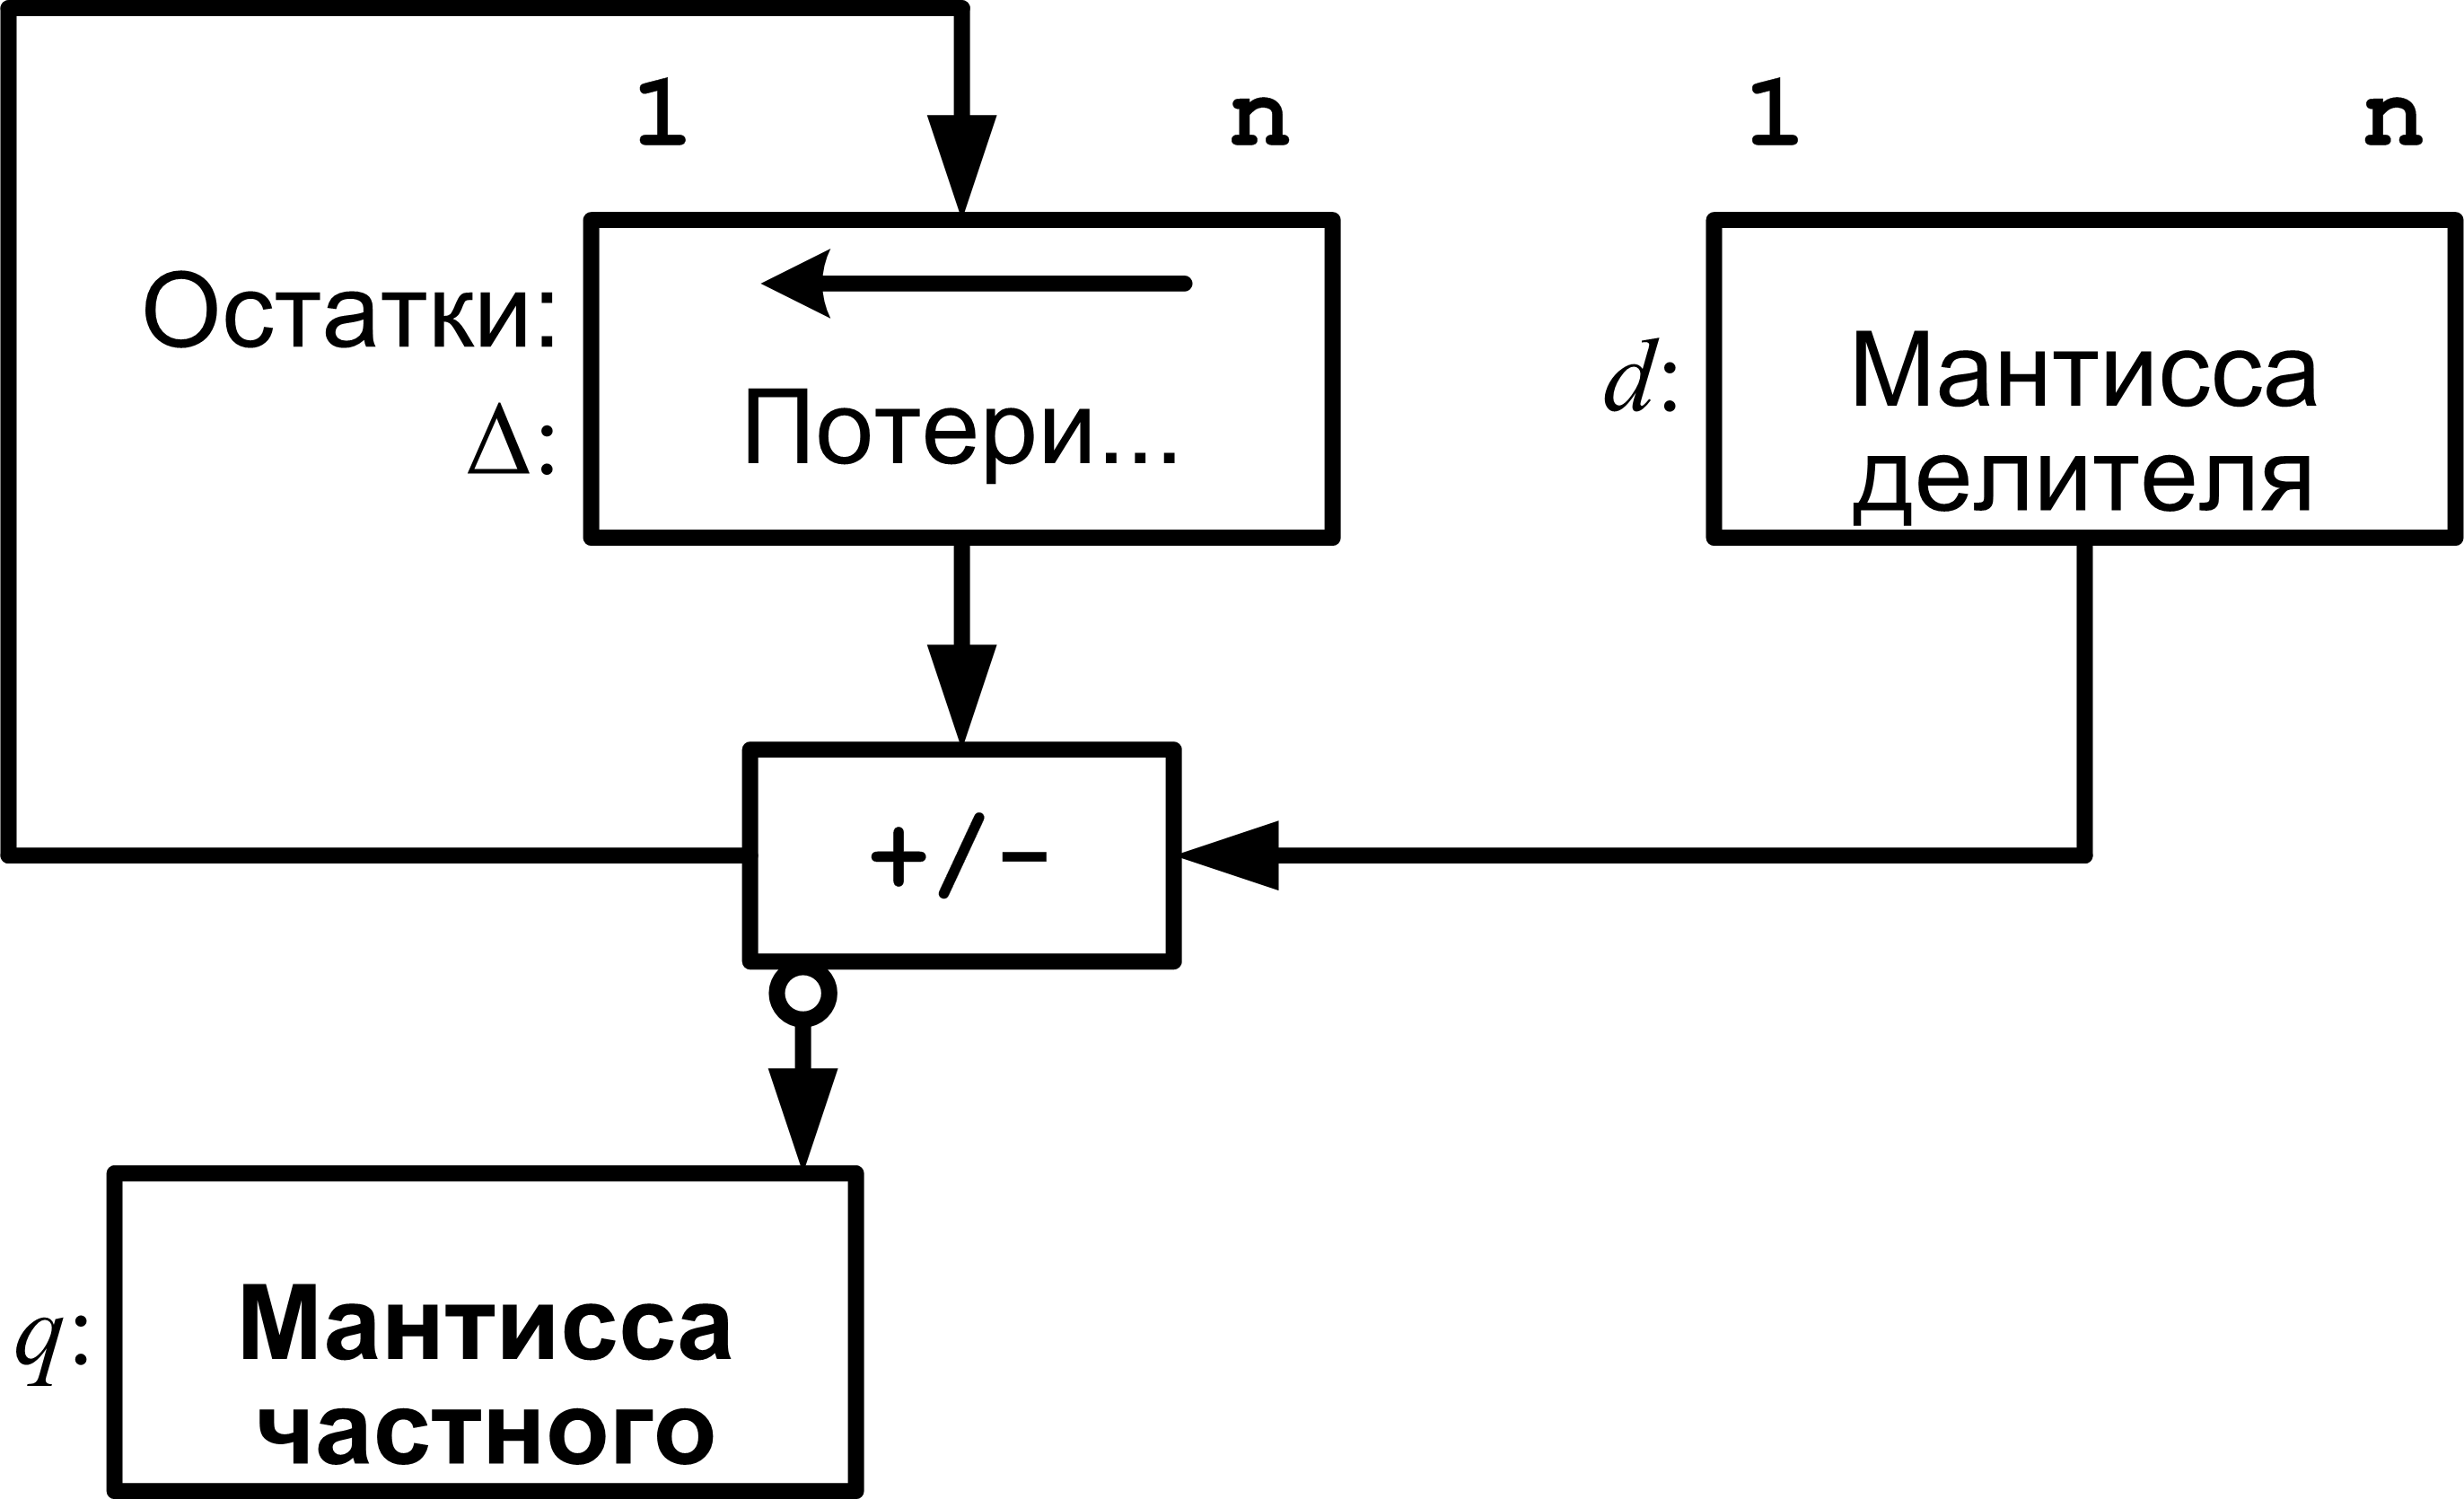
\includegraphics[width=0.47\textwidth]{fig/IFDivEnd} \\
        а) начало деления
            & б) конец деления
    \end{tabular}
    \caption{I-й способ деления нормализованных мантисс} \label{t:div:fpt:Isp}
\end{figure}

\begin{figure}[!ht]
    \centering
    \begin{tabular}{c||c}
        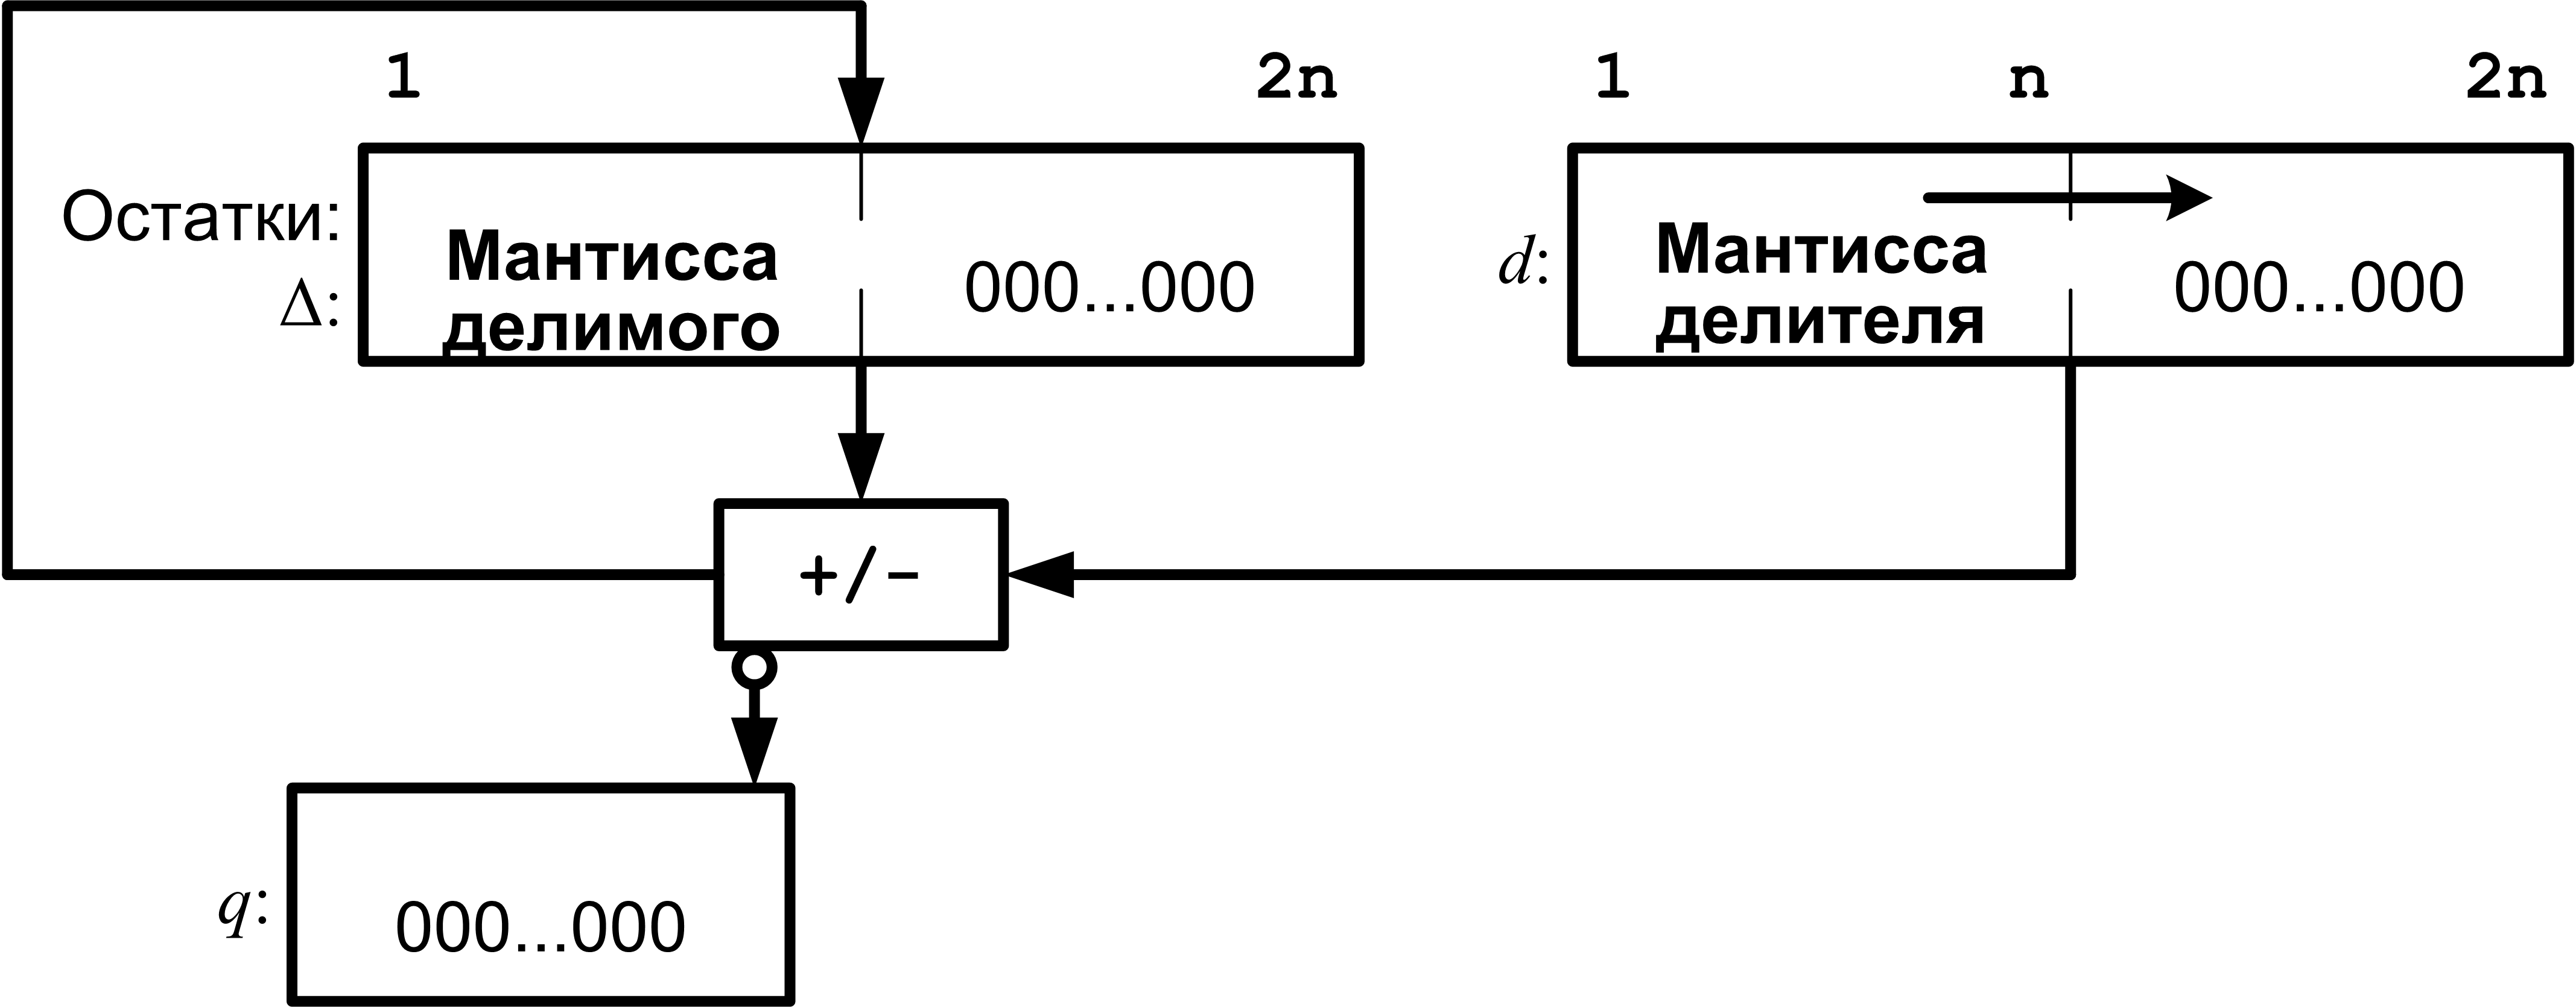
\includegraphics[width=0.47\textwidth]{fig/IIFDivBegin}
            & 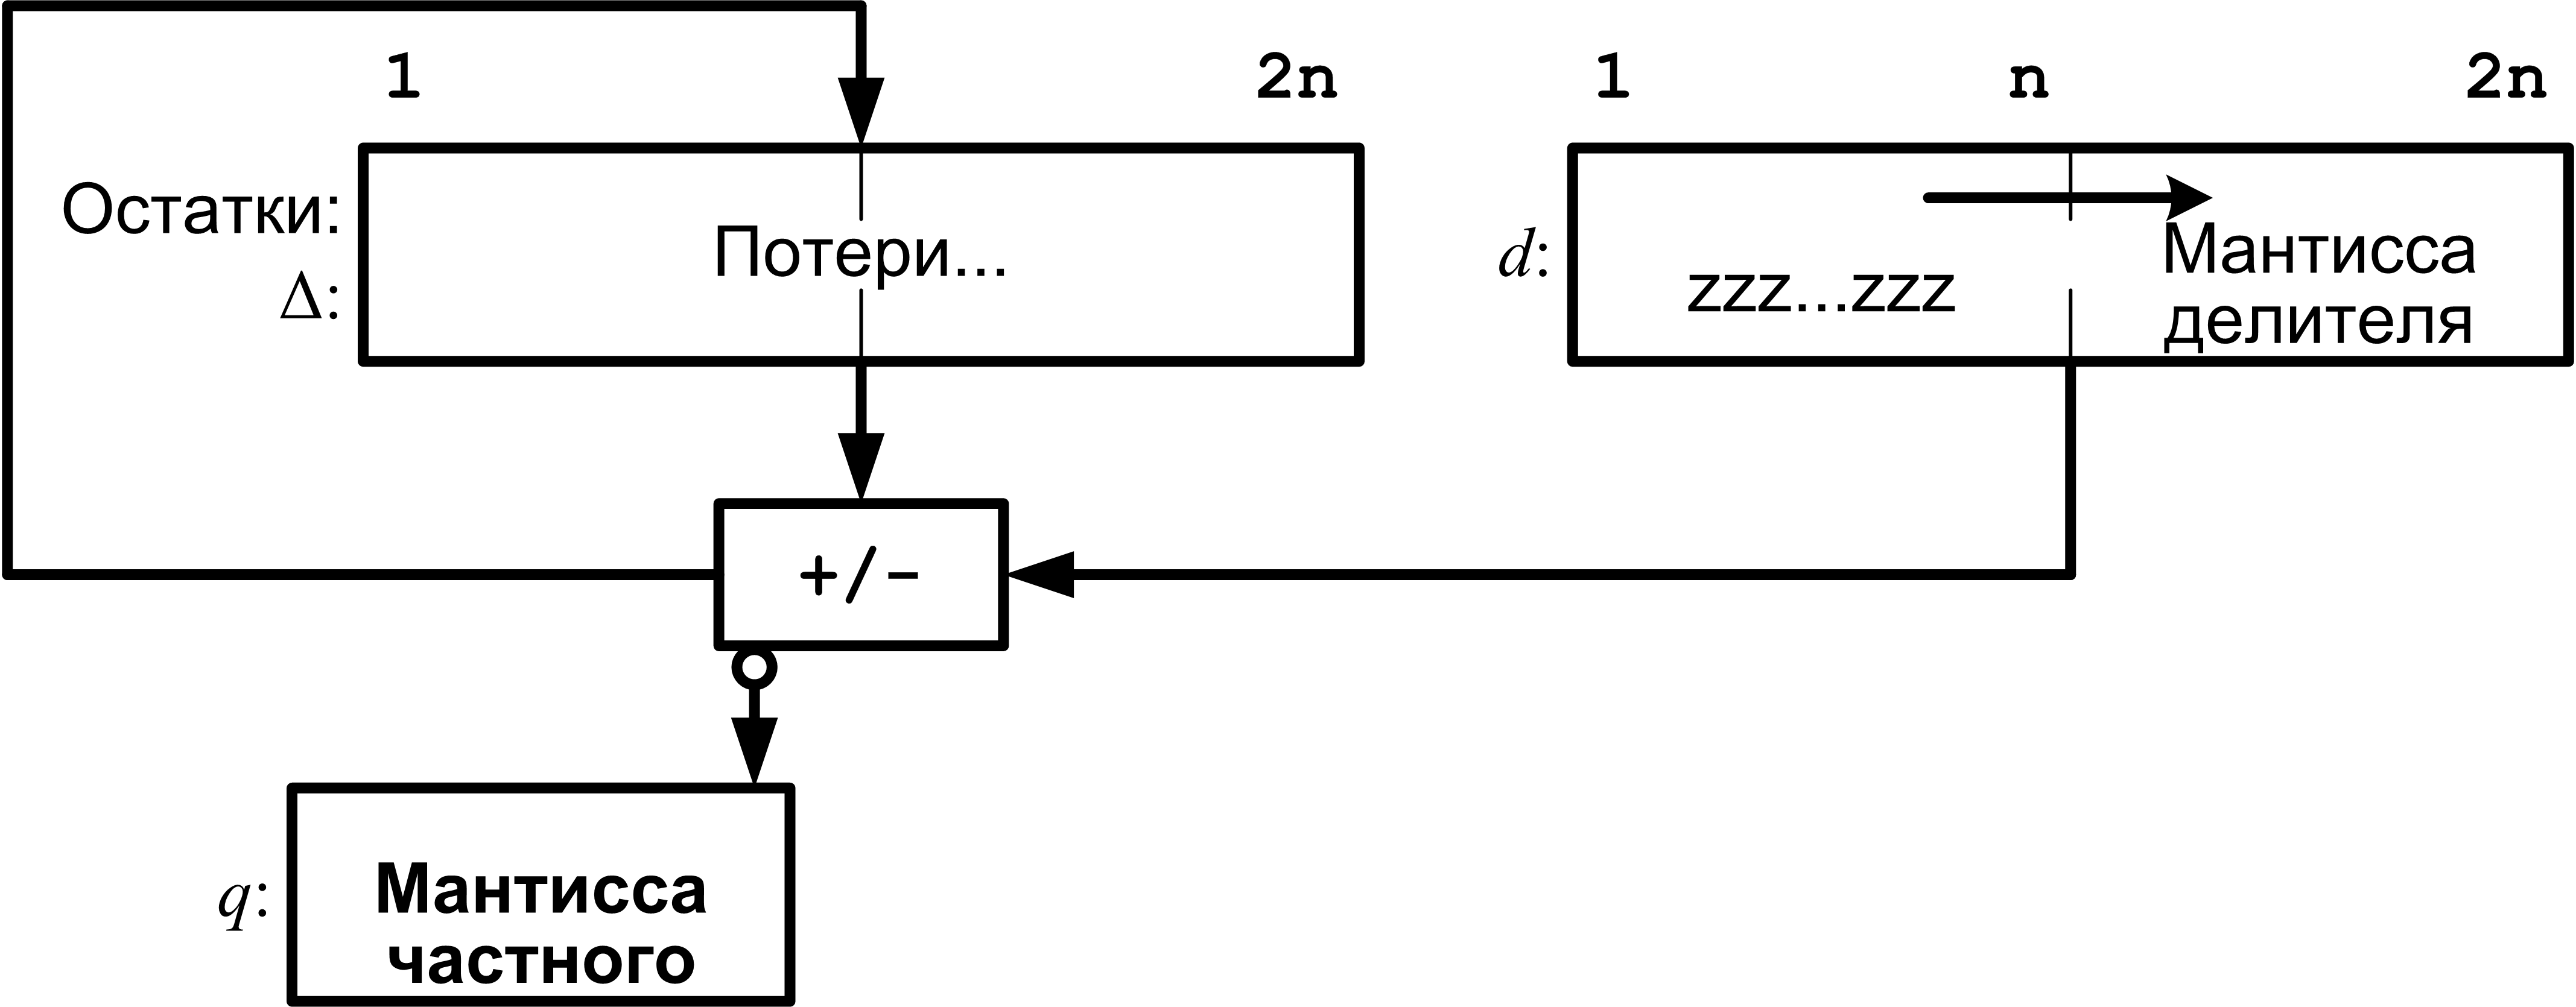
\includegraphics[width=0.47\textwidth]{fig/IIFDivEnd} \\
        а) начало деления
            & б) конец деления
    \end{tabular}
    \caption{II-й способ деления нормализованных мантисс} \label{t:div:fpt:IIsp}
\end{figure}

При делении мантисс первым способом сдвигается влево $n$-разрядный регистр остатков ($\Delta$), из значения которого в основном цикле деления вычитается значение $n$-разрядного регистра мантиссы делителя ($d$). Перед циклом деления в регистр остатков загружается делимое.

Второй способ отличается от первого тем, что регистры остатков и делителя $2n$-разрядные и сдвигается регистр делителя (вправо). В начале цикла деления мантисса делимого загружается в старшую часть регистра остатков, а делитель --- в старшую чать регистра делителя. 

Обоснование алгоритма деления мантисс без восстановления остатка аналогично обоснованию соотвествующего алгоритма для целочисленного деления. Алгоритмы с восстановлением остатка не рассматриваются, как крайне неэффективные.

Пусть формат хранит разряды модуля дробно-нормализованной мантиссы. В этом случае следует рассмотреть деление мантисс как беззнаковых дробных чисел.

Обозначим: $q$ --- частное, $\Delta$ --- остаток, $d$ --- делитель, а также соотвествующие им регистры. $A$ --- делимое.


\subsection{Деление мантисс в прямом коде}

Мантисса в прямом коде представлена знаком числа и разрядами модуля мантиссы. При этом знак и модуль мантиссы результата получаются раздельно. Знак получается сложением по <<модулю два>> (XOR) знаков операндов, а модуль мантиссы получается в результате выполнения алгоритма деления беззнаковых мантисс.

Полученный знак мантиссы в ряде случаев должен быть скорректирован, во избежание получения запрещенной в прямом коде комбинации <<отрицательного ноля>>.

\paragraph{Алгоритм деления модулей мантисс без восстановления остатков.}

\begin{enumerate}
    \item Если делитель --- ноль, фиксируется ошибка деления на ноль.
    
    \item Если делимое --- ноль, фиксируется результат: ноль.
    
    \item Вычитанием из порядка делимого порядка делителя определяется предварительный порядок частного $\OrderOf{q}\gets(\OrderOf{A}-\OrderOf{d})$. 
    
    На этом шаге может возникнуть переполнение разрядной сетки порядка. Если результат выходит за нижнюю границу представления (меньше наименьшего) то фиксируется ПМР. Ситуация ПМР может быть устранимой, когда при нормализации мантиссы увеличение порядка возвращает значение в диапазон. Если результат выходит за верхнюю границу представления (больше наибольшего), то фиксируется ПРС. Так как в процессе нормализации порядок увеличивается, то ПРС является неустранимой.
    
    \item Соотвествующим образом инициализируются регистры: остатка $\Delta$, делителя $d$, частного $q$.
    
    \item Устанавливается шаг $i\gets 0$.
    
    \item Выполняется первое вычитание делителя: $\Delta\gets(\Delta - d)$.
    
    \item Если полученный остаток $\Delta \geq 0$, то: 
    \begin{itemize}
        \item устанавливается $i\gets 1$;
        \item увеличивается на единицу предварительный порядок частного \[\OrderOf{q}\gets(\OrderOf{q} + 1);\]
        \item в младший разряд частного заносится $1$: $q_0\gets 1$.
    \end{itemize}
    
    Вследствие увеличения порядка результата может возникнуть переполнение --- в этом случае фиксируется ПРС и алгоритм завершается.
    
    \item В соответствии со схемой выполняются сдвиги регистров: $q$, $\Delta$, $d$.
    
    \item\label{fdiv:wvo:loop} Если $\Delta\ge 0$, то $\Delta\gets(\Delta - d)$, иначе $\Delta\gets(\Delta + d)$.
    
    \item Если $\Delta \ge 0$, то в младший разряд частного заносится 1, иначе --- 0. Т.е. \[q_0\gets \overline{sign(\Delta)}.\]
    
    \item Выполняется переход к следующему шагу $i\gets (i + 1)$. Если $i\geq n$, то к шагу \ref{fdiv:wvo:end}.
    
    \item В соответствии со схемой выполняются сдвиги регистров: $q$, $\Delta$, $d$ и к шагу \ref{fdiv:wvo:loop}.
    
    \item\label{fdiv:wvo:end} Определяется знак результата по знаковым разрядам операндов. Выдается результат: $\FloatExpression{q}{2}$. 
\end{enumerate}

До выдачи результата может быть выполнено округление (не обязательный, но желательный шаг).
\paragraph{Алгоритм округления.}
\begin{enumerate}
    \item Получается еще один остаток $\Delta$ (см. шаг основного алгоритма \ref{fdiv:wvo:loop}).
    
    \item Если $\Delta\ge 0$, то мантисса частного инкрементируется. Если при этом из старшего разряда мантиссы возникает перенос, то мантисса нормализуется сдвигом вправо и порядок результата увеличивается. При этом  может возникнуть ПРС порядка и вычисления завершатся ошибкой.
\end{enumerate}

\begin{Example}
    Разделить $A=-22$ на $d=9$ в формате с плавающей запятой. Для представления чисел использовать следующий формат:
    \[\FloatMyOrderX{X}{XXXXX}{X}{XXX},\]
    где в разрядах $[9:4]$ представлен прямой код мантиссы, а в разрядах $[3:0]$ --- порядок числа.
\end{Example}
\begin{Solve}
    В заданном формате числа будут представляться так:
    
    \begin{align*}
        A=-22 & \Leftrightarrow & \FloatMyOrderX{1}{10110}{0}{101}\\
          d=9 & \Leftrightarrow & \FloatMyOrderX{0}{10010}{0}{100}
    \end{align*}
    
    Предварительный порядок частного $q=\frac{A}{d}$ будет $\OrderOf{q}=5-4=1$.
    
    Деление модулей мантисс отражено в таблице \ref{t:div:fpt:IspPc}. Таблица совмещает сразу оба способа деления, так как разряды частного получаются в той же последовательности.
    
    В первом способе к регистру остатка добавлено два разряда под знак, чтобы не терять знак остатка после сдвига регистра.
    
    Во втором способе к регистрам делителя и остатка добавлен разряд справа --- это сделано только для округления, чтобы полностью избежать потерь в точности при сдвиге делителя (при отсечении добавлять разряд необязательно). 
    
    Видно, что в данном примере добавленный разряд вообще не заполняется значащим разрядом делителя. Это происходит потому, что первое вычитание делителя дает положительный остаток и потому основной цикл деления сокращается на один шаг. Если этого не сделать, то мантисса частного получится не нормализованной.
    
    Из приведенной таблицы видно, что на первом шаге получен положительный остаток, вследствие чего скорректирован порядок результата и уменьшено на единицу число шагов основного цикла деления. Таким образом выполняется нормализация результата до окончания основного цикла.
    
    \begin{figure}[!ht]
        \centering
        \begin{tabular}{c||r||r|r||l}
            \hline\hline
                & \multicolumn{1}{c||}{I-способ}
                    & \multicolumn{2}{c||}{II-способ}
                        & \\ 
            $q, \leftarrow$ 
                & \multicolumn{1}{c||}{$\Delta, \leftarrow$}
                    & \multicolumn{1}{c|}{$\Delta$}
                        & \multicolumn{1}{c||}{$d, \rightarrow$}
                            & прим.\\ 
            \hline\hline
            \Number{.....}
                & \Number{..,10110}
                    & \Number{.,10110 ..... .}
                        & \Number{.,10010 ..... .}
                            & Исх. данные.\\ \hline\hline
            \Number{....1}
                & \Addition{00,10110}
                           {11,01110}
                           {00,00100}
                    & \Addition{0,10110 ..... .}
                               {1,01110 ..... .}
                               {0,00100 00000 0}
                        & \Number{.,10010 ..... .}
                            & \Stack{$-d$; $\Delta_0>0$;}{
                                    \Stack{$\OrderOf{q}\gets(\OrderOf{q}+1)$;}{
                                        $i\gets (i+1)$;
                                    }
                              }
                              \\ \hline
            \Number{...10}
                & \Addition{00,0100.}
                           {11,01110}
                           {11,10110}
                    & \Addition{0,00100 00000 0}
                               {1,10111 0.... .}
                               {1,11011 00000 0}
                        & \Number{.,.1001 0.... .}
                            &$-d$; $\Delta_1<0$; \\ \hline
            \Number{..100}
                & \Addition{11,0110.}
                           {..,10010}
                           {11,11110}
                    & \Addition{1,11011 00000 0}
                               {.,..100 10... .}
                               {1,11111 10000 0}
                        & \Number{.,..100 10... .}
                            & $+d$; $\Delta_2<0$; \\ \hline
            \Number{.1001}
                & \Addition{11,1110.}
                           {..,10010}
                           {00,01110}
                    & \Addition{1,11111 10000 0}
                               {.,...10 010.. .}
                               {0,00001 11000 0}
                        & \Number{.,...10 010.. .}
                            & $+d$; $\Delta_3>0$; \\ \hline
            \Number{10011}
                & \Addition{00,1110.}
                           {11,01110}
                           {00,01010}
                    & \Addition{0,00001 11000 0}
                               {1,11110 1110. .}
                               {0,00000 10100 0}
                        & \Number{.,....1 0010. .}
                            & \Stack{$-d$; $\Delta_4>0$;}{
                                    Р-т отсеч.!
                              } \\ \hline\hline
            \Addition{10011}{....1}{10100}
                & \Addition{00,1010.}
                           {11,01110}
                           {00,00010}
                    & \Addition{0,00000 10100 0}
                               {1,11111 01110 .}
                               {0,00000 00010 0}
                        & \Number{.,..... 10010 .}
                            & \Stack{$-d$; $\Delta_5>0$;}{$\MantissOf{q}\gets(\MantissOf{q}+1)$;}\\ \hline
            \Number{10100}
                & 
                    &
                        &
                            & \Stack{Р-т округл.!}{$\OrderOf{q}=2$.}\\ 
        \end{tabular}
        
        \caption{Деление мантисс $\frac{-22}{9}$ I/II-сп без восстановления остатков}
        \label{t:div:fpt:IspPc}
    \end{figure}
    
    Результат с отсечением:
    \[\FloatMyOrderX{1}{10011}{0}{010}\]
    равный $-2.375$, дает абсолютную погрешность:
    \[\left|\frac{22}{9}-\frac{19}{8}\right|=\frac{5}{72}.\]
    
    Результат с округлением:
    \[\FloatMyOrderX{1}{10100}{0}{010}\]
    равный $-2.5$, дает абсолютную погрешность:
    \[\left|\frac{22}{9}-\frac{20}{8}\right|=\frac{4}{72}.\]
    
    Округление результата дает б\'{о}льшую точность.
\end{Solve}

\begin{Example}
    Разделить $A=21$ на $d=25$ в формате с плавающей точкой. Для представления чисел использовать следующий формат:
    \[\FloatMyCharX{X}{XXXXX}{XXXX},\]
    где в разрядах $[9:4]$ представлен прямой код мантиссы, а в разрядах $[3:0]$ --- характеристика (смещенный порядок) числа.
\end{Example}
\begin{Solve}
    В заданном формате числа будут представляться так:
    
    \begin{align*}
        A=21 & \Leftrightarrow & \FloatMyCharX{0}{10101}{1101}\\
        d=25 & \Leftrightarrow & \FloatMyCharX{0}{11001}{1101}
    \end{align*}
    
    Предварительная характеристика частного $q=\frac{A}{d}$ будет $\CharOf{q}=\CharOf{A}-\CharOf{d}+8=13-13+8=8$.
    
    Деление модулей мантисс отражено в таблице \ref{t:div:fpt:IspIIspPc}, совмещающей сразу оба способа деления.
    
    Из приведенной таблицы видно, что на первом шаге получен отрицательный остаток, а значит мантисса частного получается нормализованной и увеличения предварительной характеристики частного не требуется.
    
    \begin{figure}[!ht]
        \centering
        \begin{tabular}{c||r||r|r||l}
            \hline\hline
                & \multicolumn{1}{c||}{I-способ}
                    & \multicolumn{2}{c||}{II-способ}
                        & \\ 
            $q, \leftarrow$ 
                & \multicolumn{1}{c||}{$\Delta, \leftarrow$}
                    & \multicolumn{1}{c|}{$\Delta$}
                        & \multicolumn{1}{c||}{$d, \rightarrow$}
                            & прим.\\ 
            \hline\hline
            \Number{.....}
                & \Number{..,10101}
                    & \Number{.,10101 ..... .}
                        & \Number{.,11001 ..... .}
                            & Исх. данные.\\ \hline\hline
            \Number{....0}
                & \Addition{00,10101}
                           {11,00111}
                           {11,11100}
                    & \Addition{0,10101 ..... .}
                               {1,00111 ..... .}
                               {1,11100 00000 0}
                        & \Number{.,11001 ..... .}
                            &$-d$; $\Delta_0<0$; \\ \hline
            \Number{...01}
                & \Addition{11,1100.}
                           {00,11001}
                           {00,10001}
                    & \Addition{1,11100 00000 0}
                               {.,.1100 1.... .}
                               {0,01000 10000 0}
                        & \Number{.,.1100 1.... .}
                            &$+d$; $\Delta_0>0$; \\ \hline
            \Number{..011}
                & \Addition{01,0001.}
                           {11,00111}
                           {00,01001}
                    & \Addition{0,01000 10000 0}
                               {1,11001 11... .}
                               {0,00010 01000 0}
                        & \Number{.,..110 01... .}
                            &$-d$; $\Delta_1>0$; \\ \hline
            \Number{.0110}
                & \Addition{00,1001.}
                           {11,00111}
                           {11,11001}
                    & \Addition{0,00010 01000 0}
                               {1,11100 111.. .}
                               {1,11111 00100 0}
                        & \Number{.,...11 001.. .}
                            &$-d$; $\Delta_2<0$; \\ \hline
            \Number{01101}
                & \Addition{11,1001.}
                           {00,11001}
                           {00,01011}
                    & \Addition{1,11111 00100 0}
                               {.,....1 1001. .}
                               {0,00000 10110 0}
                        & \Number{.,....1 1001. .}
                            &$+d$; $\Delta_3>0$; \\ \hline
            \Number{11010}
                & \Addition{00,1011.}
                           {11,00111}
                           {11,11101}
                    & \Addition{0,00000 10110 0}
                               {1,11111 00111 .}
                               {1,11111 11101 0}
                        & \Number{.,..... 11001 .}
                            &\Stack{$-d$; $\Delta_4<0$;}{Р-т отсеч.!}\\ \hline\hline
            \Addition{11010}
                     {....1}
                     {11011}
                & \Addition{11,1101.}
                           {00,11001}
                           {00,10011}
                    & \Addition{1,11111 11101 0}
                               {.,..... .1100 1}
                               {0,00000 01001 1}
                        & \Number{.,..... .1100 1}
                            &$+d$; $\Delta_5>0$; \\ \hline
            \Number{11011}
                & 
                    & 
                        & 
                            & \Stack{Р-т округл.!}{$\CharOf{q}=8$;} 
        \end{tabular}
        
        \caption{Деление мантисс $\frac{21}{25}$ I/II-способами без восстановления остатков}
        \label{t:div:fpt:IspIIspPc}
    \end{figure}
    
    Результат с отсечением:
    \[\FloatMyCharX{0}{11010}{1000}\]
    равный $0.8125$, дает абсолютную погрешность:
    \[\left|\frac{21}{25}-\frac{26}{32}\right|=\frac{22}{800}.\]
    
    Результат с округлением:
    \[\FloatMyCharX{0}{11011}{1000}\]
    равный $0,84375$, дает абсолютную погрешность:
    \[\left|\frac{21}{25}-\frac{27}{32}\right|=\frac{3}{800}.\]
    
    Округление результата дает б\'{о}льшую точность.
\end{Solve}


\subsection{Деление мантисс в дополнительном коде}

Особенности представления чисел в формате с плавающей точкой, который использует мантиссу в дополнительном коде, отражены в примере \ref{ch:digitFormat:16DcMantChar}.

При делении мантисс желательно получить мантиссу частного сразу в дополнительном коде. Этого можно достичь, если проанализировать, что происходит с модулем остатка при вычитании делителя.
\begin{enumerate}
    \item Если после очередного действия знак остатка $\Delta$ совпадает со знаком делимого $A$, то это значит, что определяемый разряд частного $q_0$ --- единица, в противном случае --- ноль. 
    
    \[q_0\gets(sign(A)\leftrightarrow sign(\Delta))\]
    
    Здесь логическая функция тождества $(a\leftrightarrow b)$, возвращает истину, когда $(a=b)$, а функция $sign(x)$ возвращает знак числа $x$:
    \[
        sign(x)=
        \begin{cases}
            0, & x \geq 0, \\
            1, & x < 0.
        \end{cases}
    \]
    
    \item Если знаки делимого $A$ и делителя $d$ различаются, то частное $q$ должно получиться отрицательным, и в этом случае полученный в предыдущем пункте разряд $q_0$ следует инвертировать. С такой задачей прекрасно справляется функция XOR ($a\oplus b$):
    \[q_0\gets (q_0\oplus \lnot(sign(A)\leftrightarrow sign(d))).\]
    
    Строго говоря, в этом случае будет получаться обратный, а не дополнительный код частного. Далее будет показано, как, выполнив округление, можно получить правильный результат.
\end{enumerate}

Таким образом, логическое выражение для $q_0$:
\[((sign(A)\leftrightarrow sign(\Delta))\oplus \lnot(sign(A)\leftrightarrow sign(d))).\]

Используя основные тождества для функции XOR:
\begin{align*}
    (a\leftrightarrow b) & = \lnot(a\oplus b),\\
    (a\oplus b)          & = \lnot(a\leftrightarrow b),\\
    (a\oplus 0)          & = a,\\
    (a\oplus 1)          & = \lnot a,\\
    (a\oplus a)          & = 0,\\
\end{align*}
логическое выражение для $q_0$ существенно упрощается:
\begin{align*}
    ((sign(A)\leftrightarrow sign(\Delta))\oplus \lnot(sign(A)\leftrightarrow sign(d)))=\\
    =(\lnot(sign(A)\oplus sign(\Delta))\oplus (sign(A)\oplus sign(d)))=\\
    =(1\oplus sign(A) \oplus sign(\Delta) \oplus sign(A)\oplus sign(d))=\\
    =(1\oplus sign(\Delta) \oplus sign(d))=\\
    =\lnot(sign(\Delta) \oplus sign(d))=\\
    =(sign(\Delta) \leftrightarrow sign(d)).\\
\end{align*}

Таким образом, в текущий разряд частного следует записать единицу, если знак остатка совпадает со знаком делителя, и ноль --- в противном случае:
\[
    q_0\gets(sign(\Delta) \leftrightarrow sign(d)).
\]


\paragraph{Процедура поиска разряда частного.}

Вызов: $\text{ШАГ}(\Delta,d,q)$

Ввод: $\Delta$ --- значение регистра остатка, $d$ --- значение мантиссы делителя, $q$ --- значение мантиссы частного,

Вывод: $\Delta,q$ --- изменяют свое значение регистры остатка и частного.

\begin{enumerate}
    \item Если знак остатка $\Delta$ и делителя $d$ совпадают, то $\Delta\gets(\Delta-d)$, иначе $\Delta\gets(\Delta+d)$.
    \[
        \Delta\gets
            \begin{cases}
                (\Delta-d), & \text{ если $sign(\Delta)\leftrightarrow sign(d)$},\\
                (\Delta+d), & \text{ иначе}.
            \end{cases}
    \]
    
    \item Определяется значение младшего разряда мантиссы частного: $1$, если знаки остатка $\Delta$ и делителя $d$ совпадают, иначе --- $0$.
    \[
        q_0\gets(sign(\Delta) \leftrightarrow sign(d)).
    \]
    Значение подается на вход замещения младшего разряда регистра мантиссы частного $q$.
    
    \item В соответствии со схемой выполняются сдвиги регистров: $q$, $\Delta$, $d$.
\end{enumerate}


\paragraph{Алгоритм деления мантисс в дополнительном коде без восстановления остатков.}

\begin{enumerate}
    \item Если делитель --- ноль, фиксируется ошибка деления на ноль.
    
    \item Если делимое --- ноль, фиксируется результат: ноль.
    
    \item Вычитанием из порядка делимого порядка делителя определяется предварительный порядок частного $\OrderOf{q}\gets(\OrderOf{A}-\OrderOf{d})$.
    
    На этом шаге может возникнуть ситуации ПМР (как устранимого, так и неустранимого) и неустранимого ПРС.
    
    \item \label{fdiv:dc:init} Соотвествующим образом инициализируются регистры остатка $\Delta$ и делителя $d$. Младший разряд регистра частного $q_0$ заполняются знаком будущего результата: $q_0\gets (sign(A)\oplus sign(d))$.

    \item Устанавливается шаг $i\gets 1$.
    
    \item \label{fdiv:dc:loop} Выполняется процедура поиска разряда частного:
    \[
        \text{ШАГ}(\Delta,d,q).
    \]
    
    \item $i\gets (i + 1)$. Если $i < n$, то выполняется переход к пункту \ref{fdiv:dc:loop}.
    
    \item В основном цикле были определены $(n-1)$ разрядов мантиссы частного. Старший (знаковый) разряд мантиссы частного был определен на шаге \ref{fdiv:dc:init}.
    
    \item Если на данном этапе старшая пара разрядов мантиссы имеет значения \Machine{01} или \Machine{10} (то есть мантисса оказалась нормализованной), то предварительный порядок частного следует увеличить на единицу $\OrderOf{q}\gets(\OrderOf{q} + 1)$ и выполнить переход к шагу \ref{fdiv:dc:end}. При увеличении порядка может возникнуть ситуация ПРС.
    
    \item Иначе, если старшая пара разрядов мантиссы имеет значения \Machine{00} или \Machine{11}, то следует выполнить еще один шаг основного цикла, чтобы определить очередной разряд мантиссы частного:
    \[
        \text{ШАГ}(\Delta,d,q).
    \]

    На этом шаге коррекции порядка $\OrderOf{q}$ не требуется, а мантисса после сделанного шага должна нормализоваться автоматически.
    
    \item \label{fdiv:dc:end} Фиксируется ошибка или выдается результат: $\FloatExpression{q}{2}$. 
    
    Мантисса частного на данном шаге, строго говоря, получается в обратном коде, но при большой разрядности разница (погрешность) оказывается невелика. Чтобы уменьшить погрешность вычислений, можно выполнить округление.
\end{enumerate}

Если снять ограничение на количество шагов в данном алгоритме и ограничения размерности регистров схемы деления, то технически можно получить сколь угодно много разрядов мантиссы частного. Пусть разрядность мантиссы $n$-бит и требуется грамотно выполнить округление:

\[
    .\underbrace{\overbrace{xx\cdots xx}^{\MantissOf{q}}}_n xx\cdots
\]

Обобщенно, результаты деления могут быть следующими (см. также особенности округления дополнительных кодов в разделе \ref{ch::float::ss::round}).
\begin{itemize}
    \item В случае положительного результата
    \[.\overbrace{0x\cdots xx}^{\MantissOf{q}} xx\cdots\]
    достаточно рассмотреть следующие случаи:
    
    \begin{itemize}
        \item $.\overbrace{0x\cdots xx}^{\MantissOf{q}} 0x\cdots$.
        
        Отбрасываемая часть начинается с нуля. В этом случае поправок не требуется.

        \item $.\overbrace{0x\cdots xx}^{\MantissOf{q}} 1x\cdots$.
        
        В этом случае требуется поправка $\MantissOf{q}\gets(\MantissOf{q}+1)$.
    \end{itemize}
    
    \item В случае отрицательного результата
    \[.\overbrace{1x\cdots xx}^{\MantissOf{q}} xx\cdots\]
    следует рассмотреть следующие случаи:
    
    \begin{itemize}
        \item $.\overbrace{1x\cdots xx}^{\MantissOf{q}} 00\cdots 0\cdots$.
        
        В отбрасываемой части нули. Ситуация возникает при делении на положительный делитель, а на $i$-м шаге основного цикла получается нулевой остаток. Результат получен в дополнительном коде и поправок не требует.
        
        \item $.\overbrace{1x\cdots xx}^{\MantissOf{q}} 0x\cdots x1x\cdots$.
        
        Старший разряд отбрасываемой части --- нуль, а за ним следует произвольная последовательность, в которой встречаются и единицы и нули. В этом случае отбрасываемая часть модуля мантиссы начинается с единицы и требуется получить:
        \[
            -(\overline{\MantissOf{q}}+1)=-(-\MantissOf{q}-1+1)=\MantissOf{q}.
        \]
        
        Поправок не требуется.
        
        \item $.\overbrace{1x\cdots xx}^{\MantissOf{q}} 10\cdots 0\cdots$.
        
        Старший разряд отбрасываемой части --- 1, а все последующие разряды --- нули. Такая комбинация разрядов на выходе не возникнет.

        \item $.\overbrace{1x\cdots xx}^{\MantissOf{q}} 11\cdots 1\cdots$.
        
        В отбрасываемой части все единицы. Такая ситуация возникает, когда выполняется деление на отрицательный делитель и на $i$-м шаге основного цикла в остатке образуется ноль. 
        
        В этом случае требуется поправка $\MantissOf{q}\gets(\MantissOf{q}+1)$.
        
        \item $.\overbrace{1x\cdots xx}^{\MantissOf{q}} 1x\cdots x1x\cdots$.
        
        В старшем разряде отбрасываемой части --- 1, далее следет произвольная последовательность в которой встречаются и единицы и нули. В этом случае отбрасываемая часть модуля мантиссы начинается с нуля и требуется получить:
        \[-(\overline{\MantissOf{q}})=-(-\MantissOf{q}-1)=(\MantissOf{q}+1).\]
        
        Требуется поправка: $\MantissOf{q}\gets(\MantissOf{q}+1)$.
        
    \end{itemize}
\end{itemize}

\begin{Rule}
    Если отбрасываемая часть начинается с единицы, то мантиссу округляемого частного следует увеличить на единицу.
\end{Rule}


\paragraph{Алгоритм округления.}
\begin{enumerate}
    \item Выполняется поиск старшего разряда отбрасываемой части. Для этого можно выполнить процедуру поиска разряда частного:
    \[
        \text{ШАГ}(\Delta,d,q),
    \]
    но не выполнять сдвиг регистра частного.
    
    \item Если найденный старший разряд отбрасываемой части --- ноль, то алгоритм завершается, коррекции мантиссы не требуется.
    
    \item В противном случае мантисса результата увеличивается на единицу. Это действие может повлечь одно из следующих взаимоисключающих последствий.
    \begin{itemize}
        \item Если мантисса до округления была положительной, то после инкремента может возникнуть временное ПРС мантиссы. Для коррекции мантисса сдвигается вправо, а порядок увеличивается на единицу. Возможно ПРС.
        
        \item Если мантисса до округления была отрицательной, то после инкремента может наступить потеря нормализации. Для коррекции мантисса сдвигается влево, а порядок на единицу уменьшается. Возможно ПМР.
        
        \item Ни ПРС мантиссы, ни потери нормализации не возникнет. Никаких действий по коррекции не требуется.
    \end{itemize}
\end{enumerate}

\begin{Example}
    Разделить $A=-23$ на $d=19$ в формате с плавающей запятой. Для представления чисел использовать следующий формат:
    \[\FloatMyDcOrderX{XXXXXX}{X}{XXX},\]
    где в разрядах $[9:4]$ представлен дополнительный код мантиссы, а в разрядах $[3:0]$ --- порядок числа.
\end{Example}
\begin{Solve}
    В заданном формате числа будут представляться так (см. особенности представления в примере \ref{ch:digitFormat:16DcMantChar}):
    
    \begin{align*}
        A=-23 & \Leftrightarrow & \FloatMyDcOrderX{101001}{0}{101}\\
         d=19 & \Leftrightarrow & \FloatMyDcOrderX{010011}{0}{101}
    \end{align*}
    
    Предварительный порядок частного $q=\frac{A}{d}$ будет $\OrderOf{q}=5-5=0$.
    
    Деление модулей мантисс отражено в таблице \ref{t:div:fpt:DcRounding}.
    
    В первом способе к регистру остатка добавлен разряд под знак, чтобы не терять знак остатка после сдвига регистра.
    
    Во втором способе к регистрам делителя и остатка добавлен разряд справа --- это сделано только для округления, чтобы полностью избежать потерь в точности при сдвиге делителя. Видно, что в данном примере добавленный разряд вовсе не заполняется значащим разрядом делителя --- это происходит из-за того, что после $(n-1)$ шагов основного цикла, выполняются условия нормализации мантиссы и поэтому не выполняется поиск $n$-го разряда частного.

    Из приведенной таблицы видно, что уже на $5$-м шаге цикла мантисса оказалась нормализованной. Такая ситуация означает, что результат получается <<с целой частью>>, и поэтому предварительный порядок $\OrderOf{q}$ увеличивается на единицу.
    
    \begin{figure}[!ht]
        \centering
        \begin{tabular}{c||r||r|r||l}
            \hline\hline
                & \multicolumn{1}{c||}{I-способ}
                    & \multicolumn{2}{c||}{II-способ}
                        & \\ 
            $q, \leftarrow$ 
                & \multicolumn{1}{c||}{$\Delta, \leftarrow$}
                    & \multicolumn{1}{c|}{$\Delta$}
                        & \multicolumn{1}{c||}{$d, \rightarrow$}
                            & прим.\\ 
            \hline\hline
            \Number{.,....1}
                & \Number{11,01001}
                    & \Number{1,01001 ..... .}
                        & \Number{.,10011 ..... .}
                            & Исх. данные.\\ \hline\hline
            \Number{.,...10}
                & \Addition{11,01001}
                           {..,10011}
                           {11,11100}
                    & \Addition{1,01001 ..... .}
                               {.,10011 ..... .}
                               {1,11100 00000 0}
                        & \Number{.,10011 ..... .}
                            & \Stack{$+d$;}{$s(\Delta_1)\not= s(d)$;}
                              \\ \hline
            \Number{.,..101}
                & \Addition{11,1100.}
                           {..,10011}
                           {00,01011}
                    & \Addition{1,11100 00000 0}
                               {.,.1001 1.... .}
                               {0,00101 10000 0}
                        & \Number{.,.1001 1.... .}
                            &\Stack{$+d$;}{$s(\Delta_2)= s(d)$;} \\ \hline
            \Number{.,.1011}
                & \Addition{00,1011.}
                           {11,01101}
                           {00,00011}
                    & \Addition{0,00101 10000 0}
                               {1,11011 01... .}
                               {0,00000 11000 0}
                        & \Number{.,..100 11... .}
                            & \Stack{$-d$;}{$s(\Delta_3)= s(d)$;} \\ \hline
            \Number{.,10110}
                & \Addition{00,0011.}
                           {11,01101}
                           {11,10011}
                    & \Addition{0,00000 11000 0}
                               {1,11101 101.. .}
                               {1,11110 01100 0}
                        & \Number{.,...10 011.. .}
                            & \Stack{$-d$;}{$s(\Delta_4)\not= s(d)$;} \\ \hline
            \Number{1,01100}
                & \Addition{11,0011.}
                           {..,10011}
                           {11,11001}
                    & \Addition{1,11110 01100 0}
                               {.,....1 0011. .}
                               {1,11111 10010 0}
                        & \Number{.,....1 0011. .}
                            & \StackFour{$+d$;}
                                        {$s(\Delta_5)\not= s(d)$;}
                                        {$\OrderOf{q}\gets(\OrderOf{q} + 1)$}
                                        {Р-т отсеч.!}
                                \\ \hline\hline
            \Addition{1,01100}{.,....1}{1,01101}
                & \Addition{11,1001.}
                           {00,10011}
                           {00,00010}
                    & \Addition{1,11111 10010 0}
                               {.,..... 10011 .}
                               {0,00000 00101 0}
                        & \Number{.,..... 10011 .}
                            & \StackThree{$+d$;}
                                         {$s(\Delta_6)= s(d)$;}
                                         {$\MantissOf{q}\gets(\MantissOf{q}+1)$;}\\ \hline
            \Number{1,01101}
                & 
                    &
                        &
                            & \Stack{Р-т округл.!}{$\OrderOf{q}=1$.}\\ 
        \end{tabular}
        
        \caption{Деление мантисс $\frac{-23}{19}$ в дополнительном коде I/II-сп без восстановления остатков}
        \label{t:div:fpt:DcRounding}
    \end{figure}
    
    Результат с отсечением:
    \[\FloatMyDcOrderX{101100}{0}{001}\]
    равный $-1.25$, дает абсолютную погрешность:
    \[\left|\frac{23}{19}-\frac{20}{16}\right|=\frac{12}{304}.\]
    
    Результат с округлением:
    \[\FloatMyDcOrderX{101101}{0}{001}\]
    равный $-1.1875$, дает абсолютную погрешность:
    \[\left|\frac{23}{19}-\frac{19}{16}\right|=\frac{7}{304}.\]
    
    Округление в дополнительном коде позволяет получать результат с меньшей погрешностью, а также без погрешности в случае <<деления нацело>>, когда на некотором шаге основного цикла деления получается нулевой остаток.
\end{Solve}

\begin{Example}
    Разделить $A=21$ на $d=-25$ в формате с плавающей запятой. Для представления чисел использовать следующий формат:
    \[\FloatMyDcCharX{XXXXXX}{XXXX},\]
    где в разрядах $[9:4]$ представлен дополнительный код мантиссы, а в разрядах $[3:0]$ --- характеристика числа.
\end{Example}
\begin{Solve}
    В заданном формате числа будут представляться так (см. особенности представления в примере \ref{ch:digitFormat:16DcMantChar}):
    
    \begin{align*}
        A=21  & \Leftrightarrow & \FloatMyDcCharX{010101}{1101}\\
        d=-25 & \Leftrightarrow & \FloatMyDcCharX{100111}{1101}
    \end{align*}
    
    Предварительная характеристика частного $q=\frac{A}{d}$ будет $\CharOf{q}=13-13+8=0$.
    
    Деление модулей мантисс отражено в таблице \ref{t:div:fpt:DcUnRounding}.
    
    Из приведенной таблицы видно, что на $5$-м шаге цикла мантисса оказалась ненормализованной поэтому выполняется процедура поиска разряда частного и на $6$-м шаге процесс завершается автоматической нормализацией мантиссы.
    
    \begin{figure}[!ht]
        \centering
        \begin{tabular}{c||r||r|r||l}
            \hline\hline
                & \multicolumn{1}{c||}{I-способ}
                    & \multicolumn{2}{c||}{II-способ}
                        & \\ 
            $q, \leftarrow$ 
                & \multicolumn{1}{c||}{$\Delta, \leftarrow$}
                    & \multicolumn{1}{c|}{$\Delta$}
                        & \multicolumn{1}{c||}{$d, \rightarrow$}
                            & прим.\\ 
            \hline\hline
            \Number{.,....1}
                & \Number{00,10101}
                    & \Number{0,10101 ..... .}
                        & \Number{1,00111 ..... .}
                            & Исх. данные.\\ \hline\hline
            \Number{.,...11}
                & \Addition{00,10101}
                           {11,00111}
                           {11,11100}
                    & \Addition{0,10101 ..... .}
                               {1,00111 ..... .}
                               {1,11100 00000 0}
                        & \Number{1,00111 ..... .}
                            & \Stack{$+d$;}{$s(\Delta_1)= s(d)$;}
                              \\ \hline
            \Number{.,..110}
                & \Addition{11,1100.}
                           {00,11001}
                           {00,10001}
                    & \Addition{1,11100 00000 0}
                               {.,.1100 1.... .}
                               {0,01000 10000 0}
                        & \Number{1,10011 1.... .}
                            &\Stack{$-d$;}{$s(\Delta_2)\not= s(d)$;} \\ \hline
            \Number{.,.1100}
                & \Addition{01,0001.}
                           {11,00111}
                           {00,01001}
                    & \Addition{0,01000 10000 0}
                               {1,11001 11... .}
                               {0,00010 01000 0}
                        & \Number{1,11001 11... .}
                            & \Stack{$+d$;}{$s(\Delta_3)\not= s(d)$;} \\ \hline
            \Number{.,11001}
                & \Addition{00,1001.}
                           {11,00111}
                           {11,11001}
                    & \Addition{0,00010 01000 0}
                               {1,11100 111.. .}
                               {1,11111 00100 0}
                        & \Number{1,11100 111.. .}
                            & \Stack{$+d$;}{$s(\Delta_4)= s(d)$;} \\ \hline
            \Number{1,10010}
                & \Addition{11,1001.}
                           {00,11001}
                           {00,01011}
                    & \Addition{1,11111 00100 0}
                               {.,....1 1001. .}
                               {0,00000 10110 0}
                        & \Number{1,11110 0111. .}
                            & \StackThree{$-d$;}
                                        {$s(\Delta_5)\not= s(d)$;}
                                        {Ещё шаг!}
                                \\ \hline
            \Number{1,00101}
                & \Addition{00,1011.}
                           {11,00111}
                           {11,11101}
                    & \Addition{0,00000 10110 0}
                               {1,11111 00111 .}
                               {1,11111 11101 0}
                        & \Number{1,11111 00111 .}
                            & \StackThree{$+d$;}
                                        {$s(\Delta_6)= s(d)$;}
                                        {Р-т отсеч.!}
                                \\ \hline\hline
            \Addition{1,00101}{.,....0}{1,00101}
                & \Addition{11,1101.}
                           {00,11001}
                           {00,10011}
                    & \Addition{1,11111 11101 0}
                               {0,00000 01100 1}
                               {0,00000 01001 1}
                        & \Number{1,11111 10011 1}
                            & \Stack{$-d$;}
                                    {$s(\Delta_7)\not= s(d)$;}
                                \\ \hline
            \Number{1,00101}
                & 
                    &
                        &
                            & \Stack{Р-т округл.!}{$\CharOf{q}=8$.}\\ 
        \end{tabular}
        
        \caption{Деление мантисс $\frac{21}{-25}$ в дополнительном коде I/II-сп без восстановления остатков}
        \label{t:div:fpt:DcUnRounding}
    \end{figure}
    
    Результат с отсечением совпадает с округленным результатом:
    \[\FloatMyDcCharX{100101}{1000}\]
    равный $-0.84375$, дает абсолютную погрешность:
    \[\left|\frac{21}{-25}-\frac{-27}{32}\right|=\frac{3}{800}.\]
    
    Непосредственной проверкой можно убедиться, что ближайшие варианты с той же характеристикой:
    \begin{align*}
        \FloatMyDcCharX{100100}{1000}\\
        \FloatMyDcCharX{100110}{1000}
    \end{align*}
    дают б\'{о}льшую погрешность.
\end{Solve}


\subsection{Исходы операции деления}

%Исходы в формате с плавающей запятой --- обсудить отдельно в формате с плавающей запятой.

ПРС, возникает, когда результат вычитания порядков операндов выходит за пределы представления \emph{положительных} порядков. При делении ситуация ПРС является неустранимой, так как в процессе нормализации порядок результата может только увеличиваться. В случае ПРС фиксируется ошибка вычислений.

ПМР, возникает, когда результат вычитания порядков операндов выходит за пределы представления \emph{отрицательных} порядков. При делении ситуация ПМР может оказаться устранимой, так как в процессе нормализации порядок результата может увеличиваться и порядок результата при этом может <<вернуться>> в диапазон. В случае ПМР --- в качестве результата выдается ноль и фиксируется ситуация ПМР (например, устанавливается соотвествущий флаг).
 %деление чисел в формате с плавающей точкой
          %деление двоичных чисел
    \chapter{Сложение двоично-десятичных чисел}
\label{ch:bcd}


\newcommand{\NaturalLabel}{\text{``\texttt{8421}''}}
\newcommand{\Natural}[1]{\NaturalLabel(#1)}

\newcommand{\PlusThreeLabel}{\text{``\texttt{8421+3}''}}
\newcommand{\PlusThree}[1]{\PlusThreeLabel(#1)}

\newcommand{\AikenLabel}{\text{``\texttt{2421}''}}
\newcommand{\Aiken}[1]{\AikenLabel(#1)}

\newcommand{\PentaLabel}{\text{``\texttt{3a+2}''}}
\newcommand{\Penta}[1]{\PentaLabel(#1)}


Двоично-десятичный код используется для представления десятичных цифр. Сложение же выполняется по правилам десятичной арифметики, только вместо сложения десятичных цифр выполняется сложение кодов. Далее рассматривается сложение в десятичной системе счисления.

Обратный код в десятичной системе счисления получается следующим образом:
\[
    \OC{X} = 
    \begin{cases}
        \overline{|X|}, &\text{ если $X<0$,}\\
        |X|,            &\text{ если $X\ge 0$,}
    \end{cases}
\]
где $\overline{|X|}$ --- порязрядное дополнение цифр десятичного числа $X$ до $9$, то есть разряд $x_i$ числа находится как $(9-x_i)$.    

Восстановление числа со знаком из обратного кода выполняется следующим образом.
\[
    X = 
    \begin{cases}
        -(\overline{\OC{X}}), &\text{ если $msb(\OC{X})=9$,}\\
         \OC{X},              &\text{ если $msb(\OC{X})=0$,}
    \end{cases}
\]
где $msb(x)$ --- функция, возвращающая старший значащий бит последовательности $x$.    

При сложении единицу переноса из старшего разрядя следует прибавить к младшему разряду.

\begin{Example}
    Сложить числа $527$ и ${-365}$ в 4-х рязрядной десятичной сетке.
\end{Example}
\begin{Solve}
    Выполним дробное масштабирование $M=10^4$ и переведем числа в обратный код:
    \begin{align*}
        \OC{527} &=\Number{,0527},\\
        \OC{-365}&=\Number{,9634}.
    \end{align*}
    
    Складываем обратные коды:
    \[
        \Addition{,0527}
                 {,9634}
                {1,0161}
    \]
    
    Поправка единицей переноса:
    \[
        \Addition{,0161}
                 {,0001}
                 {,0162}
    \]
    
    Результат: $\Number{,0162}\Rightarrow(.0162)_{10}\cdot 10^{4}=162$.
\end{Solve}

\section{Четырехбитные коды}

Для представления десятичной цифры требуется минимум 4-е двоичных разряда --- тетрада. Такое представление избыточно --- так как фактически остается еще шесть лишних значений тетрад. Следует отметить, что инверсия разрядов тетрады соответствует арифметическому дополнению значения тетрады до 15:
\[
    \overline{(\Number{xxxx})}_2 \Leftrightarrow \left((\Number{1111})_2-(\Number{xxxx})_2\right) \Leftrightarrow (15-(\Number{xxxx})_2).
\]

Например $(\Number{1001})_2=9$:
\[
    \overline{(\Number{1001})}_2=(\Number{0110})_2=6=(15-9).
\]


\subsection{Код \NaturalLabel}

Код \NaturalLabel --- код с естественными весами: $\Natural{a}=a$. То есть значение тетрады кода совпадает с десятичной цифрой. Кодирование приведено в таблице \ref{t:bcd:Natural}.

\begin{table}[!ht]
    \caption{Код \NaturalLabel}
    \label{t:bcd:Natural}
    \centering
    \begin{tabular}{|c|c|c|}
        \hline\hline
        $a$ в 10СС  & $\Natural{a}$         & $\Natural{9-a}$\\
        \hline\hline
        $0$         & $\Number{0000}$       & $\Number{1001}$ \\
        $1$         & $\Number{0001}$       & $\Number{1000}$ \\
        $2$         & $\Number{0010}$       & $\Number{0111}$ \\
        $3$         & $\Number{0011}$       & $\Number{0110}$ \\
        $4$         & $\Number{0100}$       & $\Number{0101}$ \\
        $5$         & $\Number{0101}$       & $\Number{0100}$ \\
        $6$         & $\Number{0110}$       & $\Number{0011}$ \\
        $7$         & $\Number{0111}$       & $\Number{0010}$ \\
        $8$         & $\Number{1000}$       & $\Number{0001}$ \\
        $9$         & $\Number{1001}$       & $\Number{0000}$ \\
        \hline
    \end{tabular}
\end{table}

$\Natural{9-a}=9-a=(15-a)-6=\overline{\Natural{a}}-6=\overline{\Natural{a}}+\Number{1010}.$

Рассмотрим процесс сложения $S=A+B$, где $A=(a_{n-1}\cdots a_0)$ и $B=(b_{n-1}\cdots b_0)$. При этом $k$-й разряд суммы в 10СС получается по формуле:

\begin{equation}
    \label{eq:bcd:decAddition}
    s_k=a_k+b_k+c_k,
\end{equation}
где $c_k$ --- перенос в $k$-й разряд, а $s_k,a_k,b_k$ --- десятичные цифры.

Рассмотрим, что произойдет, если вместо десятичных цифр сложить их коды.
\begin{enumerate}
    \item $(a_k+b_k+c_k)<10$; $c_{k+1}=0$. Код $(a_k+b_k+c_k)$ корректен.
    
    \item $10\leq (a_k+b_k+c_k)\leq 15$; $c_{k+1}=0$. Неверно! Перенос в 10СС должен быть, но в 16СС его не случилось. Правильная 10СС цифра $(a_k+b_k+c_k-10)$, и перенос: $(a_k+b_k+c_k-10)+16=(a_k+b_k+c_k+6)$. Поправка: $+6=\Number{0110}$.
    
    \item $(a_k+b_k+c_k)\geq 16$; $c_{k+1}=1$. Неверно! Перенос корректен, а полученная цифра $(a_k+b_k+c_k-16)$ неправильна. Правильный код $(a_k+b_k+c_k-10)$. Поправка: $+6=\Number{0110}$. При такой поправке переноса не будет.
\end{enumerate}

Выделим из предыдущих рассуждений условия поправок и попробуем их упростить.
\begin{enumerate}
    \item\label{en:bcd:fixup} Если $0\leq(a_k+b_k+c_k)\leq 9$, то поправок не надо.
    \item Если $10\leq(a_k+b_k+c_k)\leq 19$, то нужна поправка $(+6)=\Number{0110}$. Переносы из тетрады в тетраду при этом возникают автоматически.
\end{enumerate}

Поэтому поправку $(+6)=\Number{0110}$ можно прибавить к обратному коду одного из операндов заранее. И тогда, если переноса из тетрады не будет (только в случае условия из п. \ref{en:bcd:fixup}) поправку нужно вычесть из тетрады.

Алгоритм сложения в коде {\NaturalLabel} следующий.

\begin{enumerate}
    \item Слагаемые переводятся в обратный $\NaturalLabel$-код. Каждая тетрада модуля отрицательного слагаемого инвертируются и к результату прибавляется код $(-6)=\Number{1010}$. Переносы между тетрадами при этом не распространяются.
    \item К каждой тетраде одного из слагаемых прибавляется поправка $(+6)=\Number{0110}$. Переносов между тетрадами при этом не возникает\footnote{Если одно из слагаемых отрицательно, то поправки перевода в ОК (-6) и поправка данного шага (+6) друг друга компенсируют!}.
    \item Выполняется сложение по правилам двоичной арифметики. Переносы распространяются.
    \item Корректируются тетрады, \emph{из которых} не было переносов. К каждой такой тетраде прибавляется $-6$, т.е. тетрада $\Number{1010}$. Переносы не распространяются.
    \item Результат получен в обратном \NaturalLabel-коде.
\end{enumerate}

\begin{Example}
    Cложить $637.54$ и $-48.54$.
\end{Example}
\begin{Solve}
    Используем целое масштабирование $M=10^{-2}$, $5$-и разрядную сетку и добавим слева два двоичных разряда под знак (МОК).
    \begin{enumerate}
        \item Перевод в ОК:
        \begin{align*}
            \OC{63754}=\Number{00 0110 0011 0111 0101 0100}\\
            -4854\Rightarrow-\Number{0000 0100 1000 0101 0100}\Rightarrow\\
            \Rightarrow\Addition{1111 1011 0111 1010 1011}
                                {1010 1010 1010 1010 1010}
                                {1001 0101 0001 0100 0101}\\
            \OC{-4854}=\Number{11 1001 0101 0001 0100 0101}\\
        \end{align*}
        
        \item К каждой тетраде $\OC{-4854}$ прибавлена тетрда $\Number{0110}$.
        \[
            \Addition{11 1001 0101 0001 0100 0101}
                     {.. 0110 0110 0110 0110 0110}
                     {11 1111 1011 0111 1010 1011}
        \]

        Обратите внимание, что в этом случае (когда хотя бы один из операндов отрицателен), текущая поправка $+6$ и поправка $-6$, которая прибавлялась к инверсии тетрад отрицательного числа, компенсируют друг друга. В данном случае были сделаны лишние действия, достаточно было найти инверсию тетрад $-4854$. В случае, когда оба слагаемых положительны этот шаг необходим.
        
        \item Выполняется сложение полученного числа с $\OC{63754}$. 
        \[
            \Addition{11 1111 1011 0111 1010 1011}
                     {00 0110 0011 0111 0101 0100}
                   {1*00*0101 1110 1110 1111 1111}
        \]
        Коррекция обратного кода переносом из знакового разряда:
        \[
            \Addition{00*0101 1110 1110 1111 1111}
                     {.. .... .... .... .... ...1}
                     {00*0101 1110 1111*0000*0000}
        \]

        \item Корректируются тетрады \emph{из которых не было переносов} в процессе сложения на предыдущем шаге. Переносы между тетрадами не распространяются.
        \[
            \Addition{00*0101 1110 1111*0000*0000}
                     {.. .... 1010 1010 .... ....}
                     {00 0101 1000 1001 0000 0000}
        \]
    \end{enumerate}

    ПРС не возникло, \[\OC{S}=\Number{00 0101 1000 1001 0000 0000},\] $S=58900\cdot 10^{-2}=589$.
\end{Solve}


\subsection{Код \PlusThreeLabel}

Код \PlusThreeLabel --- это код с избытком 3: $\PlusThree{a}=(a+3)$. Соответствие кодов десятичным цифрам представлено в таблице \ref{t:bcd:PlusThree}. 
    
\begin{table}[!ht]
    \caption{Код \PlusThreeLabel}
    \label{t:bcd:PlusThree}
    \centering
    \begin{tabular}{|c|c|c|}
        \hline\hline
        $a$ в 10СС  & $\PlusThree{a}$  & $\PlusThree{9-a}$\\
        \hline\hline
        $0$         & $\Number{0011}$  & $\Number{1100}$ \\
        $1$         & $\Number{0100}$  & $\Number{1011}$ \\
        $2$         & $\Number{0101}$  & $\Number{1010}$ \\
        $3$         & $\Number{0110}$  & $\Number{1001}$ \\
        $4$         & $\Number{0111}$  & $\Number{1000}$ \\
        $5$         & $\Number{1000}$  & $\Number{0111}$ \\
        $6$         & $\Number{1001}$  & $\Number{0110}$ \\
        $7$         & $\Number{1010}$  & $\Number{0101}$ \\
        $8$         & $\Number{1011}$  & $\Number{0100}$ \\
        $9$         & $\Number{1100}$  & $\Number{0011}$ \\
        \hline
    \end{tabular}
\end{table}

Двоично-десятичный код называется самодополняемым, когда в результате инверсии тетрады кода получается код дополнения исходной десятичной цифры до девяти. Код {\PlusThreeLabel} самодополняемый:
\[
    \overline{\PlusThree{a}}=15-(a+3)=12-a=(9-a)+3=\PlusThree{9-a}.
\]

При сложении кодов чисел возможны следующие случаи.

\begin{enumerate}
    \item $s_k<10$; При сложении кодов: \[(a_k+3)+(b_k+3)+c_k=(a_k+b_k+c_k)+6=(s_k+6).\] 

    Так как $(s_k+6)\leq 15$, то переноса не возникает. Правильная тетрада должна быть $(s_k+3)$, следовательно, нужна поправка $-3=\Number{1101}$. Перенос игнорируется.
    
    \item $s_k\geq 10$; При сложении кодов возникнет перенос:
    \[(a_k+3)+(b_k+3)+c_k-16=(a_k+b_k+c_k)-10=s_k-10.\] 

    Для получения правильного: $(s_k-10)+3$, нужна поправка $+3=\Number{0011}$. Перенос игнорируется.
\end{enumerate}

Алгоритм сложения по сравнению с кодов {\NaturalLabel} упрощается
    
\begin{enumerate}
    \item Слагаемые переводятся в обратный $\PlusThreeLabel$-код. Каждая тетрада модуля отрицательного числа инвертируется.
    \item Выполняется сложение полученных операднов по правилам двоичной арифметики (с распространением переносов).
    \item К тетрадам, из которых не было переноса, прибавляется $\Number{1101}$, а к остальным прибавляется $\Number{0011}$. Переносы игнорируются.
    \item Результат получен в обратном \PlusThreeLabel-коде.
\end{enumerate}

\begin{Example}
    Cложить $637.54$ и $-48.54$.
\end{Example}
\begin{Solve}
    Используем целое масштабирование в 5-и разрядной сетке: $M=10^{-2}$. 
    \begin{enumerate}
        \item Перевод в ОК (добавлены два знаковых двоичных разряда МОК):
        \begin{align*}
            -4854\Rightarrow-\Number{0011 0111 1011 1000 0111}\\
            \OC{-4854}=\Number{11 1100 1000 0100 0111 1000}\\
            \OC{63754}=\Number{00 1001 0110 1010 1000 0111}
        \end{align*}
        
        \item Выполняется сложение обратных кодов. 
        \[
            \Addition{11 1100 1000 0100 0111 1000}
                     {00 1001 0110 1010 1000 0111}
                   {1 00*0101 1110 1110 1111 1111}
        \]
        Коррекция переносом:
        \[
            \Addition{00*0101 1110 1110 1111 1111}
                     {.. .... .... .... .... ...1}
                     {00*0101 1110 1111*0000*0000}
        \]

        \item Выполняется коррекция. Переносы между тетрадами не распространяются.
        \[
            \Addition{00*0101 1110 1111*0000*0000}
                     {.. 0011 1101 1101 0011 0011}
                     {00 1000 1011 1100 0011 0011}
        \]
    \end{enumerate}
    
    ПРС не возникло, \[\OC{S}=\Number{00 1000 1011 1100 0011 0011}\] $S=58900\cdot 10^{-2}=589$.
\end{Solve}


\subsection{Код \AikenLabel}

Этот код также называется кодом Айкена, а в исходном названии отражены веса разрядов. Если в коде с естественными весами {\NaturalLabel} вклады разрядов действительно \emph{естественные}, то в коде Айкена третий разряд имеет вес $2$: 
\begin{align*}
    \Aiken{a}\equiv t_{3}t_{2}t_{1}t_{0},\\ 
    a=2t_{3}+4t_{2}+2t_{1}+1t_{0}
\end{align*}

Соответствие кодов десятичным цифрам представлено в таблице \ref{t:bcd:Aiken}. Следует обратить внимание, что одна и та же цифра может быть представлена различными кодами, например, $\Aiken{2}$ это и $\Number{0010}$, и $\Number{1000}$.
    
\begin{table}[!ht]
    \caption{Код \AikenLabel}
    \label{t:bcd:Aiken}
    \centering
    \begin{tabular}{|c|c|c|}
        \hline\hline
        $a$ в 10СС  & $\Aiken{a}$                                   & $\Aiken{9-a}$\\
        \hline\hline
        $0$         & $\Number{0000}$                               & $\Number{1111}$ \\
        $1$         & $\Number{0001}$                               & $\Number{1110}$ \\
        %                  
        $2$         & $\Number{0010}\leftrightarrow\Number{1000}$   & $\Number{1101}\leftrightarrow\Number{0111}$ \\
        $3$         & $\Number{0011}\leftrightarrow\Number{1001}$   & $\Number{1100}\leftrightarrow\Number{0110}$ \\
        $4$         & $\Number{0100}\leftrightarrow\Number{1010}$   & $\Number{1011}\leftrightarrow\Number{0101}$ \\
        $5$         & $\Number{0101}\leftrightarrow\Number{1011}$   & $\Number{1010}\leftrightarrow\Number{0100}$ \\
        $6$         & $\Number{0110}\leftrightarrow\Number{1100}$   & $\Number{1001}\leftrightarrow\Number{0011}$ \\
        $7$         & $\Number{0111}\leftrightarrow\Number{1101}$   & $\Number{1000}\leftrightarrow\Number{0010}$ \\
        %                  
        $8$         & $\Number{1110}$                               & $\Number{0001}$ \\
        $9$         & $\Number{1111}$                               & $\Number{0000}$ \\
        \hline
    \end{tabular}
\end{table}

Код Айкена самодополняем:    
\begin{align*}
    &\overline{T}=\overline{t_{3}t_{2}t_{1}t_{0}}=(2-2t_3) + (4-4t_3) + (2-2t_2) + (1-1t_0)=9-T,\\
    &\overline{\Aiken{a}} = \Aiken{9-a}.
\end{align*}

Обобщая таблицу \ref{t:bcd:Aiken}:
\begin{enumerate}
    \item если $0\leq a \leq 1$, то $\Aiken{a}=a$;
    \item если $2\leq a \leq 7$, то $\Aiken{a}=a$ или $\Aiken{a}=(a+6)$;
    \item если $8\leq a \leq 9$, то $\Aiken{a}=(a+6)$.
\end{enumerate}
    
Преследуя цель <<пусть будет>>: <<однозначность>>, <<перенос>> и <<самодополняемость>>, формулируются новые правила:
\begin{enumerate}
    \item\label{bcd:aiken:ruleI} если $0\leq a \leq 4$, то $\Aiken{a}=a$:
    \[\overline{\Aiken{a}}=(15-a)=\underbrace{(9-a)+6}_{\text{см. п. \ref{bcd:aiken:ruleII}}}=\Aiken{9-a};\]
    
    \item\label{bcd:aiken:ruleII} если $5\leq a \leq 9$, то $\Aiken{a}=(a+6)$:
    \[\overline{\Aiken{a}}=15-(a+6)=\underbrace{(9-a)}_{\text{см. п. \ref{bcd:aiken:ruleI}}}=\Aiken{9-a}.\]
\end{enumerate}

Полученное однозначное кодирование отражено в таблице \ref{t:bcd:AikenClean}.

\begin{table}[!ht]
    \caption{Код \AikenLabel}
    \label{t:bcd:AikenClean}
    \centering
    \begin{tabular}{|c|c|c|}
        \hline\hline
        $a$ в 10СС  & $\Aiken{a}$       & $\Aiken{9-a}$\\
        \hline\hline                   
        $0$         & $\Number{0000}$   & $\Number{1111}$ \\
        $1$         & $\Number{0001}$   & $\Number{1110}$ \\
        $2$         & $\Number{0010}$   & $\Number{1101}$ \\
        $3$         & $\Number{0011}$   & $\Number{1100}$ \\
        $4$         & $\Number{0100}$   & $\Number{1011}$ \\
        $5$         & $\Number{1011}$   & $\Number{0100}$ \\
        $6$         & $\Number{1100}$   & $\Number{0011}$ \\
        $7$         & $\Number{1101}$   & $\Number{0010}$ \\
        $8$         & $\Number{1110}$   & $\Number{0001}$ \\
        $9$         & $\Number{1111}$   & $\Number{0000}$ \\
        \hline
    \end{tabular}
\end{table}

Код по-прежнему самодополняем: $\overline{\Aiken{a}} = \Aiken{9-a}$.

Рассмотрим все возможные случаи, которые могут возникнуть при сложении кодов:
\begin{enumerate}
    \item Если $0\leq a_{k},b_{k}\leq 4$, то сложение кодов $(a_{k}+b_{k}+c_{k})$:
    \begin{enumerate}
        \item если $0\leq (a_{k}+b_{k}+c_{k}) \leq 4$, то поправок не нужно;
        \item если $5\leq(a_{k}+b_{k}+c_{k}) \leq 9$, то неверно! Должно быть: $(a_{k}+b_{k}+c_{k})+6$. Поправка: $+6=\Number{0110}$.
    \end{enumerate}

    \item\label{bcd:aiken:diff} Если $0\leq a_{k}\leq 4$ и $5\leq b_{k}\leq 9$, то код $(a_{k}+b_{k}+c_{k}+6)$:
    \begin{enumerate}
        \item если $5\leq (a_{k}+b_{k}+c_{k}) \leq 9$, то код верен;
        \item если $10\leq(a_{k}+b_{k}+c_{k}) \leq 14$, то формируется перенос и $(a_{k}+b_{k}+c_{k}+6)-16$. Код $(a_{k}+b_{k}+c_{k}-10)$ верен.
    \end{enumerate}
    
    \item Если $5\leq a_{k}\leq 9$ и $0\leq b_{k}\leq 4$ код верен (аналогично п.\ref{bcd:aiken:diff}).

    \item Если $5\leq a_{k},b_{k}\leq 9$, то код $(a_{k}+b_{k}+c_{k}-10)+6$:
    \begin{enumerate}
        \item если $0\leq (a_{k}+b_{k}+c_{k}-10) \leq 4$, то неверно! Должно быть: $(a_{k}+b_{k}+c_{k} - 10)$. Поправка: $-6=\Number{1010}$.
        \item если $5\leq(a_{k}+b_{k}+c_{k}-10) \leq 9$, то код верен!
    \end{enumerate}
\end{enumerate}

Выделим запрещенные комбинации кода:
\[
    \AikenLabel\notin\{\Number{0101},\Number{0110},\Number{0111},\Number{1000},\Number{1001},\Number{1010}\}.
\]
    
Сформулируем правила коррекции.
\begin{enumerate}
    \item Если $0\leq a_{k},b_{k}\leq 4$ и $5\leq(a_{k}+b_{k}+c_{k})\leq 9$, то поправка: $+6=\Number{0110}$. 
    При этом $msb(\Aiken{a_k})=msb(\Aiken{b_k})=0$ и в результате получается одна из запрещенных комбинаций.
    
    \item Если $5\leq a_{k},b_{k}\leq 9$ и $0\leq(a_{k}+b_{k}+c_{k}-10)\leq 4$, то поправка: $-6=\Number{1010}$.
    При этом $msb(\Aiken{a_k})=msb(\Aiken{b_k})=1$ и в результате получается одна из запрещенных комбинаций.
\end{enumerate}

Алгоритм сложения.
    
\begin{enumerate}
    \item Перевести слагаемые в обратный $\AikenLabel$-код. Каждая тетрада модуля отрицательного числа инвертируется.
    \item Выполняется сложение полученных операднов по правилам двоичной арифметики.
    \item Выполняется коррекция результата, в ходе которой переносы между тетрадами не распространяются. 
    Если старшие биты слагаемых тетрад, в результате сложения которых получилась запрещенная тетрада результата, имеют одинаковые значения:
    \begin{enumerate}
        \item $0$, то поправка: $+6=\Number{0110}$;
        \item $1$, то поправка: $-6=\Number{1010}$.
    \end{enumerate}
    \item Результат получен в обратном $\AikenLabel$-коде.
\end{enumerate}

\begin{Example}
    Cложить $-467.08$ и $-125.31$.
\end{Example}
\begin{Solve}
    Используем целое масштабирование в 5-и разрядной сетке: $M=10^{-2}$. 
    \begin{enumerate}
        \item Перевод в ОК (добавлены два знаковых двоичных разряда МОК):
        \begin{align*}
            -46708\Rightarrow-\Number{0100 1100 1101 0000 1110}\\
            \OC{-46708}=\Number{11 1011 0011 0010 1111 0001}\\
            -12531\Rightarrow-\Number{0001 0010 1011 0011 0001}\\
            \OC{-12531}=\Number{11 1110 1101 0100 1100 1110}\\
        \end{align*}
        
        \item Выполняется сложение обратных кодов. 
        \[
            \Addition{11 1011 0011 0010 1111 0001}
                     {11 1110 1101 0100 1100 1110}
                   {1 11 1010 0000 0111 1011 1111}
        \]
        Коррекция переносом:
        \[
            \Addition{11 1010 0000 0111 1011 1111}
                     {.. .... .... .... .... ...1}
                     {11 1010 0000 0111 1100 0000}
        \]

        \item Выполняется коррекция тетрад результата. Переносы между тетрадами не распространяются.
        \begin{align*}
            \OC{-46708}=\Number{11 1011 0011 0010 1111 0001}\\
            \OC{-12531}=\Number{11 1110 1101 0100 1100 1110}\\
                      \Addition{11 1010 0000 0111 1100 0000}
                               {.. 1010 .... 0110 .... ....}
                               {11 0100 0000 1101 1100 0000}
        \end{align*}
    \end{enumerate}
    
    ПРС не возникло, восстанавливаем результат из обратного кода.
    \begin{align*}
        \OC{S}=\Number{11 0100 0000 1101 1100 0000}\\
        \OC{|S|}=\Number{00 1011 1111 0010 0011 1111}
    \end{align*}
    $S=-59239\cdot 10^{-2}=-592.39$.
\end{Solve}


\section{Пентадный код \PentaLabel}

Пятибитный код десятичной цифры $a$ получается по следующей формуле: $\Penta{a}=(3\cdot a + 2)$. Соответствие десятичных цифр пентадам представлено в таблице \ref{t:bcd:Penta}. 
    
\begin{table}[!ht]
    \caption{Код \PentaLabel}
    \label{t:bcd:Penta}
    \centering
    \begin{tabular}{|c|c|c|}
        \hline\hline
        $a$ в 10СС  & $\Penta{a}$       & $\Penta{9-a}$\\
        \hline\hline
        $0$         & $\Number{00010}$  & $\Number{11101}$ \\
        $1$         & $\Number{00101}$  & $\Number{11010}$ \\
        $2$         & $\Number{01000}$  & $\Number{10111}$ \\
        $3$         & $\Number{01011}$  & $\Number{10100}$ \\
        $4$         & $\Number{01110}$  & $\Number{10001}$ \\
        $5$         & $\Number{10001}$  & $\Number{01110}$ \\
        $6$         & $\Number{10100}$  & $\Number{01011}$ \\
        $7$         & $\Number{10111}$  & $\Number{01000}$ \\
        $8$         & $\Number{11010}$  & $\Number{00101}$ \\
        $9$         & $\Number{11101}$  & $\Number{00010}$ \\
        \hline
    \end{tabular}
\end{table}

Пентадный код избыточен:    
\[
    \overline{\Penta{a}}=31-(3a+2)=3(9-a)+2=\Penta{9-a}
\]

Пусть $a_k$, $b_k$ --- $k$-я десятичные цифры операндов, $c_k$ --- перенос в $k$-й разряд из предыдущего.
    
\begin{enumerate}
    \item Если $0\leq a_{k}+b_{k}+c_{k}\leq 9$:
    \begin{enumerate}
        \item если $c_{k}=0$, то код $3(a_{k}+b_{k}) + 4$. Верный код: $3(a_{k}+b_{k})+2$. Поправка: $-2=\Number{11110}$:
        \item если $c_{k}=1$, то код $(3a_k+2)+(3b_{k}+2)+1=3(a_{k}+b_{k}+1)+2$. Код верен!
    \end{enumerate}

    \item Если $a_{k}+b_{k}+c_{k}\geq 10$:
    \begin{enumerate}
        \item если $c_{k}=0$, то код $(3a_{k}+2)+(3b_{k}+2)-32=3(a_{k}+ b_{k}-10)+2$. Код верен!
        \item если $c_{k}=1$, то код $(3a_{k}+2)+(3b_{k}+2)+1-32$, т.е. $3((a_{k}+b_{k}+1)-10)$. Верный код:
        $3((a_{k}+b_{k}+1)-10)+2$. Поправка: $+2=\Number{00010}$.
    \end{enumerate}
\end{enumerate}

Алгоритм сложения:

\begin{enumerate}
    \item Перевести слагаемые в обратный $\PentaLabel$-код. Каждая тетрада модуля отрицательного числа инвертируется.
    \item Выполняется сложение полученных операднов по правилам двоичной арифметики.
    \item Выполняется коррекция. Прибавляется код $11110_{2}$ к пентадам, в которые и из которых не формировались единицы переноса. Прибавляется код $00010_{2}$ к пентадам, в которые и из которых формировались единицы переноса. В процессе коррекции переносы из пентады в пентаду не распространяются.
    \item Результат получен в обратном $\PentaLabel$-коде.
\end{enumerate}

\begin{Example}
    Cложить $684.38$ и $-248.78$.
\end{Example}
\begin{Solve}
    Используем целое масштабирование в 5-и разрядной сетке: $M=10^{-2}$. 
    \begin{enumerate}
        \item Перевод в ОК (добавлены два знаковых двоичных разряда МОК):
        \begin{align*}
            \OC{68438}=\Number{00 10100 11010 01110 01011 11010}\\
            -24878\Rightarrow-\Number{01000 01110 11010 10111 11010}\\
            \OC{-12531}=\Number{11 10111 10001 00101 01000 00101}
        \end{align*}
        
        \item Выполняется сложение обратных кодов. 
        \[
            \Addition{00 10100 11010 01110 01011 11010}
                     {11 10111 10001 00101 01000 00101}
                   {1 00*01100*01011 10011 10011 11111}
        \]
        Коррекция переносом:
        \[
            \Addition{00*01100*01011 10011 10011 11111 }
                     {.. ..... ..... ..... ..... ....1 }
                     {00*01100*01011 10011 10100*00000*}
        \]

        \item Выполняется коррекция пентад результата. К пентадам в которые и из которых был перенос --- прибавляется код \Number{00010}. К пентадам в которые и из которых переноса не было --- прибавляется код \Number{11110}. К остальным пентадам поправок нет. Переносы между пентадами не распространяются.
        \begin{align*}
                      \Addition{00*01100*01011 10011 10100*00000*}
                               {.. 00010 ..... 11110 ..... 00010 }
                               {00 01110 01011 10001 10100 00010 }
        \end{align*}
    \end{enumerate}
    
    ПРС не возникло, восстанавливаем результат из обратного кода.
    \begin{align*}
        \OC{S}=\Number{00 01110 01011 10001 10100 00010}\\
    \end{align*}
    $S=43560\cdot 10^{-2}=435.6$.
\end{Solve}
          %сложение в двоично-десятичной системе
    \chapter{<<Микропрограммное управление>> --- цикл лабораторных работ}
\label{ch::practice}

Теорию построения вычислительных устройств рассмотрим на примере устройства, позволяющего выполнить тот или иной алгоритм умножения.

\begin{figure}[!ht]
    \centering
    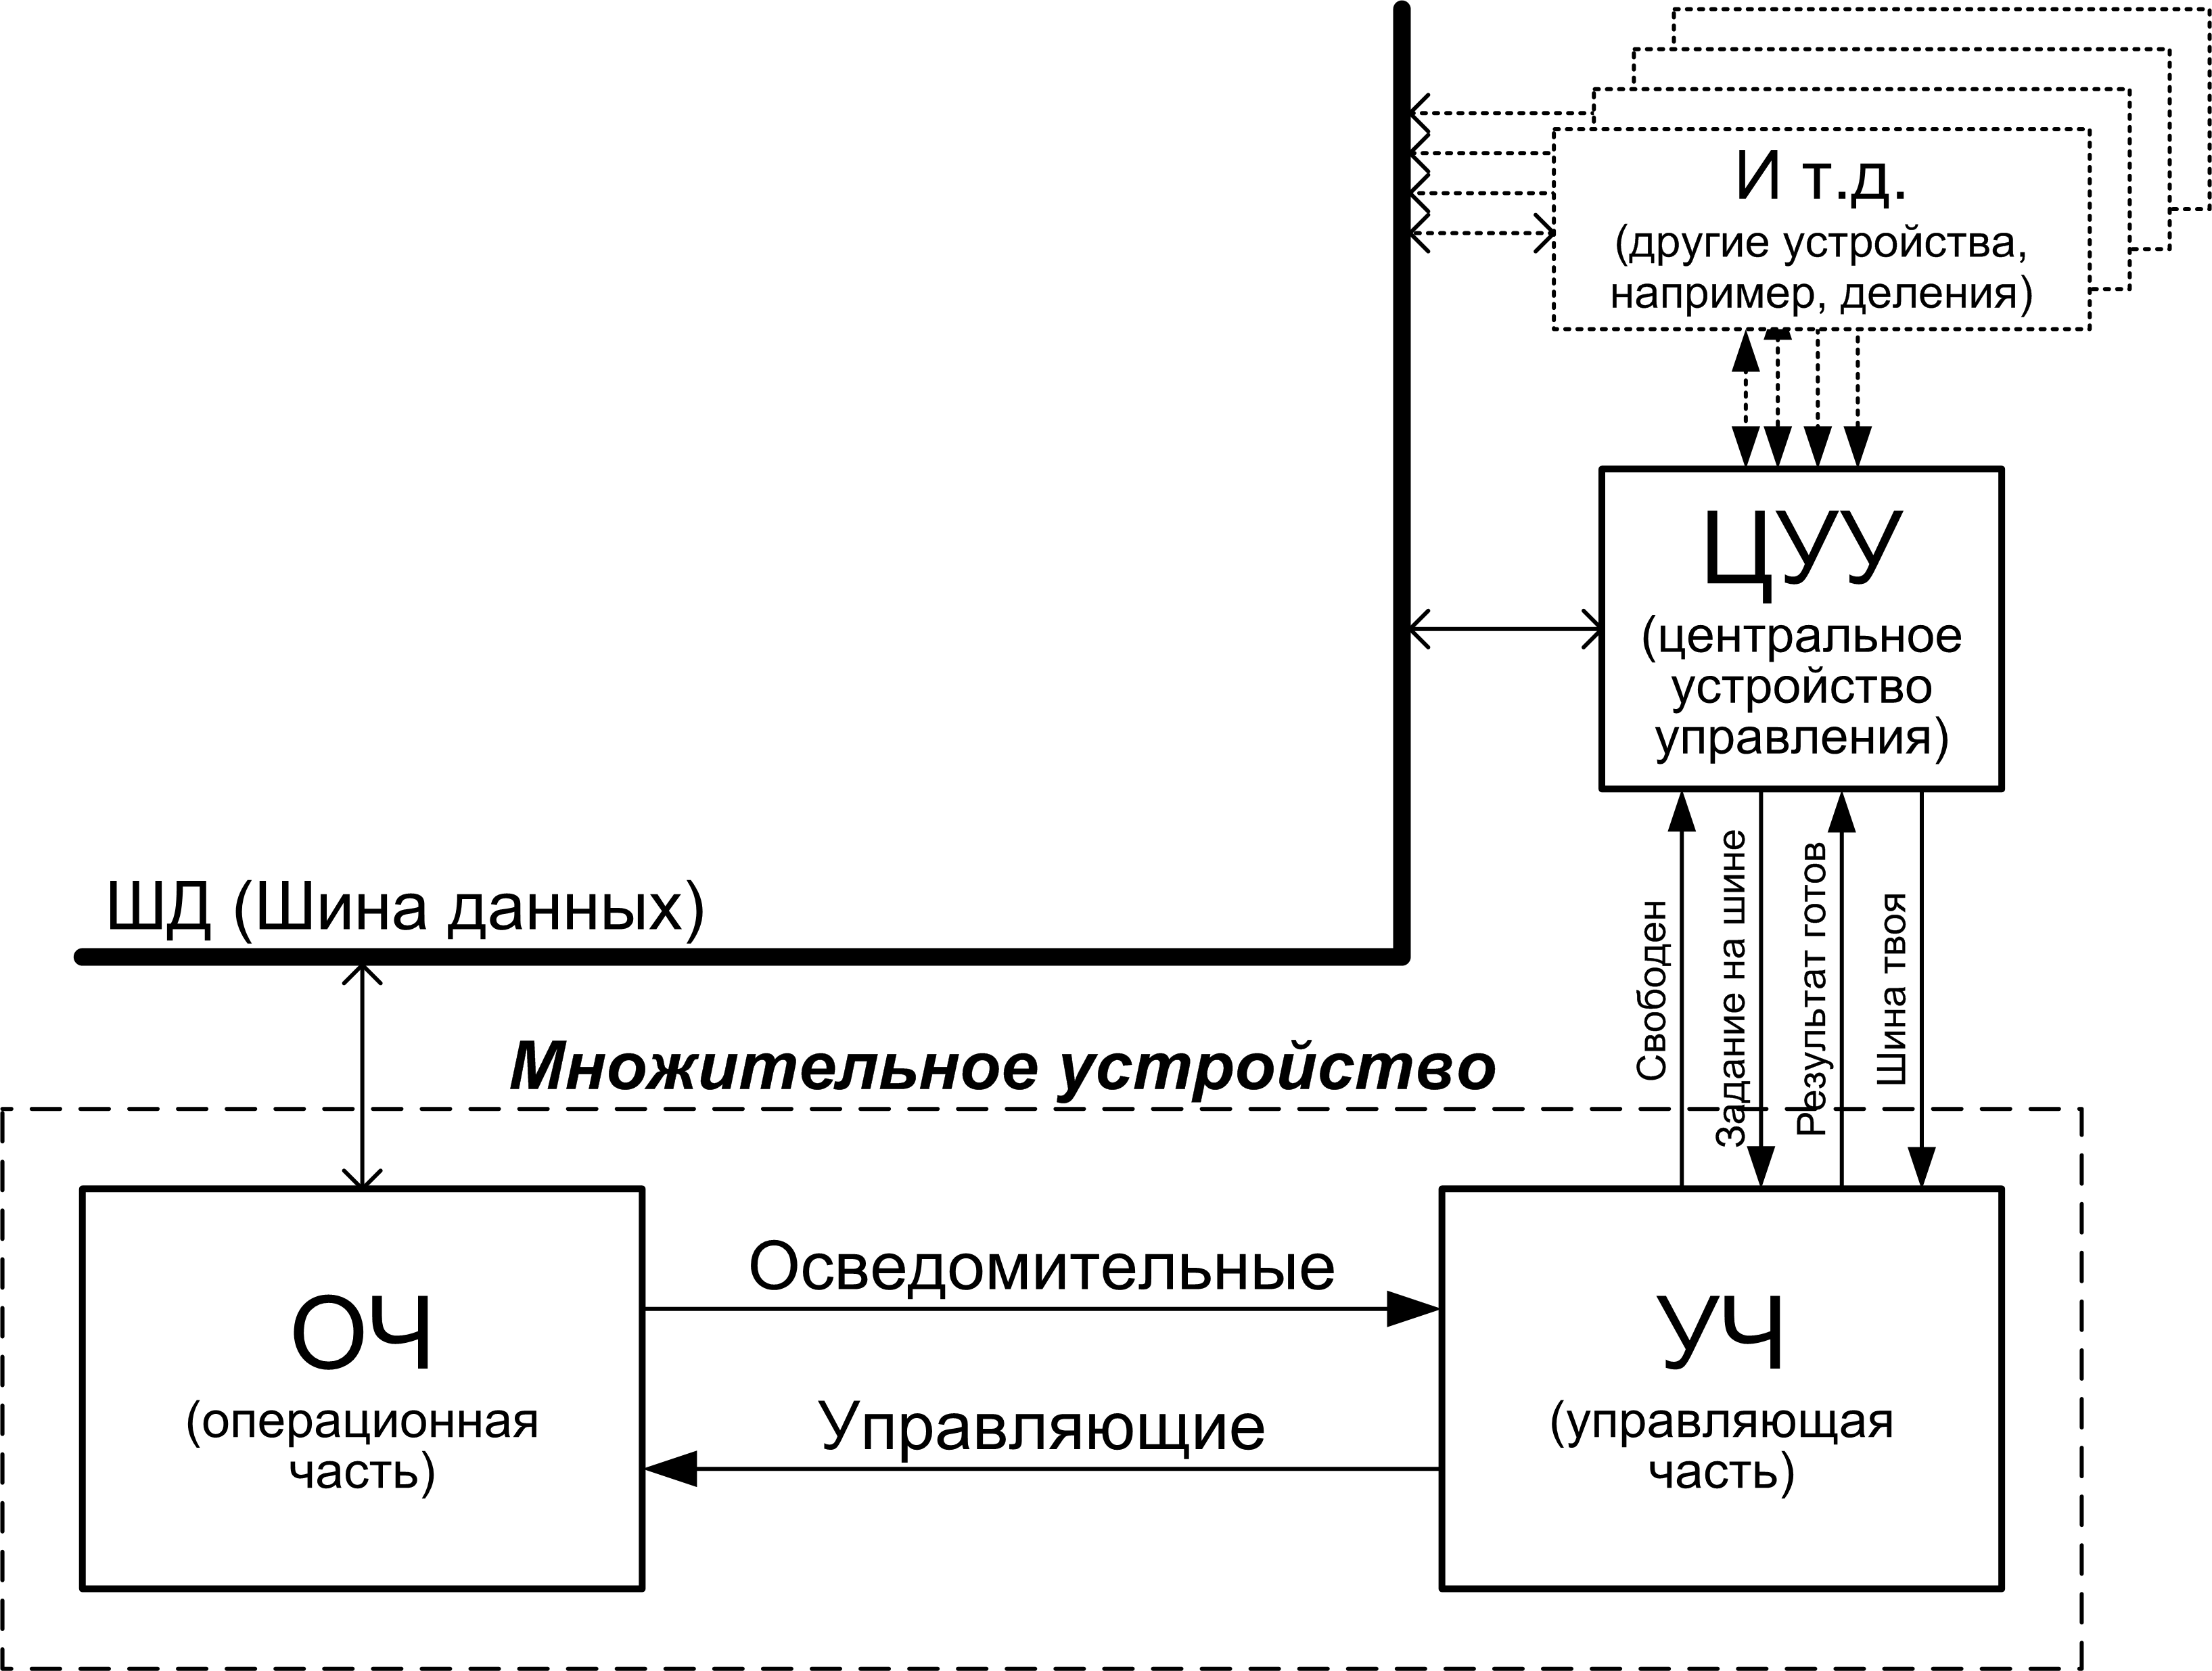
\includegraphics{fig/model}
    \caption{Структура вычислительного устройства}
    \label{fig::ch::practice::model}
\end{figure}

Структурно устройство разделяется на три компонента (см. рисунок \ref{fig::ch::practice::model}): 
\begin{itemize}
    \item центральное устройство управления (ЦУУ);
    \item операционная часть множительного устройства (ОЧ); 
    \item управляющая часть множетельного устройства (УЧ).
\end{itemize}

ЦУУ выполняет \emph{программу} пользователя, состоящую из отдельных \emph{команд}. Одной из команд является команда выполнить умножение. ЦУУ не выполняет эту операцию самсостоятельно, а дает задание множительному устройству. Множительное устройство, состоящее из операционной (ОЧ) и управляющей частей (УЧ), является лишь одним из многих устройств, которым ЦУУ перепоручает выполнить сложые операции.

Операция умножения, например, сводится к последовательности операций сложения, которые являются элементарными. Все остальные сложные операции также сводятся к выполнению элементарных операций по определенному алгоритму. \emph{Элементарная} операция выполняется некоторым элементом оборудования\footnote{Например, сложение выполняется логической схемой --- сумматором. См. описание этого элемента в разделе \ref{s::ch::practice::elements}} операционной части (ОЧ) сразу, за фиксированный (и относительно короткий) промежуток времени, называемый \emph{тактом}. В составе любого цифрового устройства имеется таймер, отсчитывающий такты\footnote{Отсюда термин \emph{тактовая частота}: $1/T$, где $T$ --- продолжительность такта}. Поэтому, когда говорится <<сложная операция>>, то подразумевается операция, выполняемая за несколько тактов.

При отсутствии сбоев, между центральным управляющим устройством (ЦУУ) и управляющей частью множительного устройства (УЧ) происходит следующий обмен синалами и данными:
\begin{enumerate}
    \item \textbf{УЧ$\to$ЦУУ:<<Свободен>>}. 
    
    УЧ выдает сигнал в ЦУУ <<Свободен>> всегда, когда не выполняет задачу. Отсутствие сигнала <<Свободен>> от УЧ трактуется ЦУУ как признак того, что множительное устройство занято решением ранее поставленной задачи.
    
    \item \textbf{ЦУУ$\to$УЧ:<<Задание на шине>>, ШД=<<Операнды>>}.

    Убедившись, что множительное устройство готово принять задание (получив от УЧ сигнал <<Свободен>>), ЦУУ выдает в УЧ сигнал <<Задание на шине>>. Передача задания по шине в общем случае может занять один или несколько тактов. Это зависит от принятых соглашений на формат передачи задания --- в общем случае это серия передач по шине данных. Получив сигнал <<Задание на шине>>, УЧ должна в следующем такте снять сигнал <<Свободен>>, и одновременно начать считывать с шины первый фрагмент задания.
    
    \item \textbf{УЧ$\to$ЦУУ:<<Результат готов>>}. 
    
    УЧ с помощью ОЧ выполняет умножение. Этот процесс может длиться довольно долго, и в это время ЦУУ может декодировать следующую команду и, если это возможно, начать её выполнять параллельно с работой мнжительного устройства. Так как при этом по шине данных (ШД) могут передаваться данные, получив результат, УЧ не должно выдавать его на шину сразу. УЧ выдает в ЦУУ осведомительный сигнал <<Результат готов>> и держит его до тех пор, пока ЦУУ не освободит шину.
    
    \item \textbf{ЦУУ$\to$УЧ:<<Шина твоя>>}. 
    
    ЦУУ, получив от УЧ сигнал <<Результат готов>>: завершает (если шина занята) текущую передачу данных по шине; выдает сигнал в УЧ <<Шина твоя>> и снимает его в следующем такте.
    
    \item \textbf{УЧ$\to$ЦУУ:ШД=<<Результат>>}. 
    
    Получив от ЦУУ сигнал <<Шина твоя>>, УЧ следующем такте должна:
    \begin{itemize}
        \item снять сигнал <<Результат готов>>;
        \item выдать на шину первый фрагмент результата, и если необходимо, продолжить в следующих тактах выдачу остальных фрагментов результата.
    \end{itemize}
\end{enumerate}

УЧ множительного устройства, выполняя алгоритм умножения, в каждом такте выдает в ОЧ необходимые управляющие сигналы. Управляющие сигналы формируются УЧ в зависимости от своего внутреннего состояния и осведомительных сигналов, часть которых поступает из ОЧ, а часть из ЦУУ. Аппаратура ОЧ содержит набор необходимых утройств, чтобы выполнить все необходимые элементарные операции.

ОЧ составлена из базовых схемотехнических цифровых элементов: логических элементов, сумматоров, мультиплексоров, триггеров, регистров, операционных усилителей и т.д. Необходимые сведения о работе этих элементов приводятся в разделе \ref{s::ch::practice::elements}.

%пришел ребенок и написал "зцуекнка Сахар словарное слово. рампмика аемпитьтлпаолдююююмпимпмвччвроолпеаакгогрипрппннпрпагшпенучвчаер"

\section{Элементы функциональной схемы}
\label{s::ch::practice::elements}

В данном разделе приводится необходимый минимум сведений для изображения и понимания функциональных схем. За исчерпывающей информацией обращайтесь к стандарту \cite{bib:gost:fs}.


\subsection{Сигналы, шины, жгуты}


Отдельная \emph{сигнальная линия} соответствует проводнику (проводу), который передает логические значения 0 или 1. Сигнальная линия на схеме изображается тонкой линией, соедняющей выход некоторого элемента со входом некоторого элемента. 

Множество внешних (интерфейсных) сигнальных линий принято объединять в \emph{шины}. Шина на схеме изображается толстой линией и обязательно именуется: сверху над линией в удобном месте подписывается имя шины (на рисунке \ref{fig::ch::practice::bus} изображена шина $X$). В общем случае шин на схеме может быть несколько. В качестве имени шины обычно выбирают заглавную литеру: $X$, $Y$, $Z$, $P$, а если шины разделены по функциональному назначению, то они могут быть названы: ШД --- шина данных, ША --- шина адреса, ШУ --- шина управления и т.д.

\begin{figure}[!ht]
    \centering
    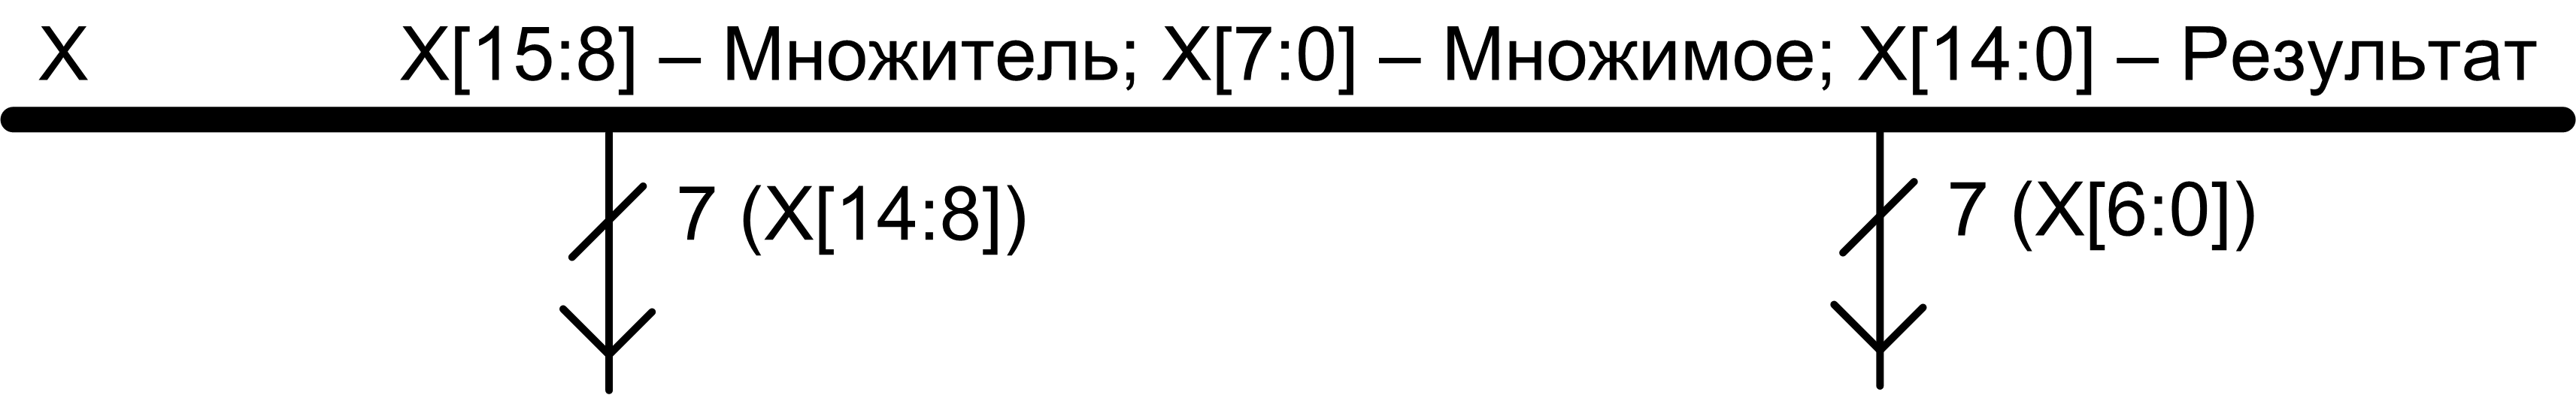
\includegraphics{fig/bus}
    \caption{Изображение шин и жгутов}
    \label{fig::ch::practice::bus}
\end{figure}

Чтобы не рисовать множество параллельных сигнальных линий, в случае, когда передается группа бит, на схеме изображают \emph{жгут}. Жгут также изображается тонкой линией, на которой в произвольном месте (но не на концах) тонкими линиями рисуется тупоугольная стрелка, указвающая направление передачи, сверху от стрелки жгут перечеркивается косой чертой и справа указывается разрядность жгута. В случае когда требуется указать, какие разряды шины отведены в жгут, в скобках после разрядности перечисляются обозначения групп сигнальных линий в составе шины. На рисунке \ref{fig::ch::practice::bus} от шины $X$ отведены два жгута по $7$ разрядов каждый.

\emph{Сигналы} разделяют на осведомительные и управляющие. Управляющие сигналы обычно обозначаются: $Y0$, $Y1$, $Y2$,\ldots, а осведомительные --- $P0$, $P1$, $P2$,\ldots Если управляющий сигнал подается на вход элемента, а не на управление, то стрелку не рисуют.  На рисунке \ref{fig::ch::practice::controls} изображен $8$-и разрядный регистр (подробнее о регистрах см. раздел \ref{sss::ch::practice::regiter}), который управляется сигналами $Y0$, $Y1$. Седьмой разряд выхода регистра используется как осведомительный сигнал $P0$. На входные разряды с $0$ по $3$ подаются соответственно сигналы с $3$ по $6$ шины $X$. На вход $RG1[7:4]$ подается двоичное значение $(0011)_2$.

Управляющие сигналы подводятся стрелками, входящими в управляемый блок справа. Осведомительные отводятся с выходов стрелкой, направленной вниз или влево.

\begin{figure}[!ht]
    \centering
    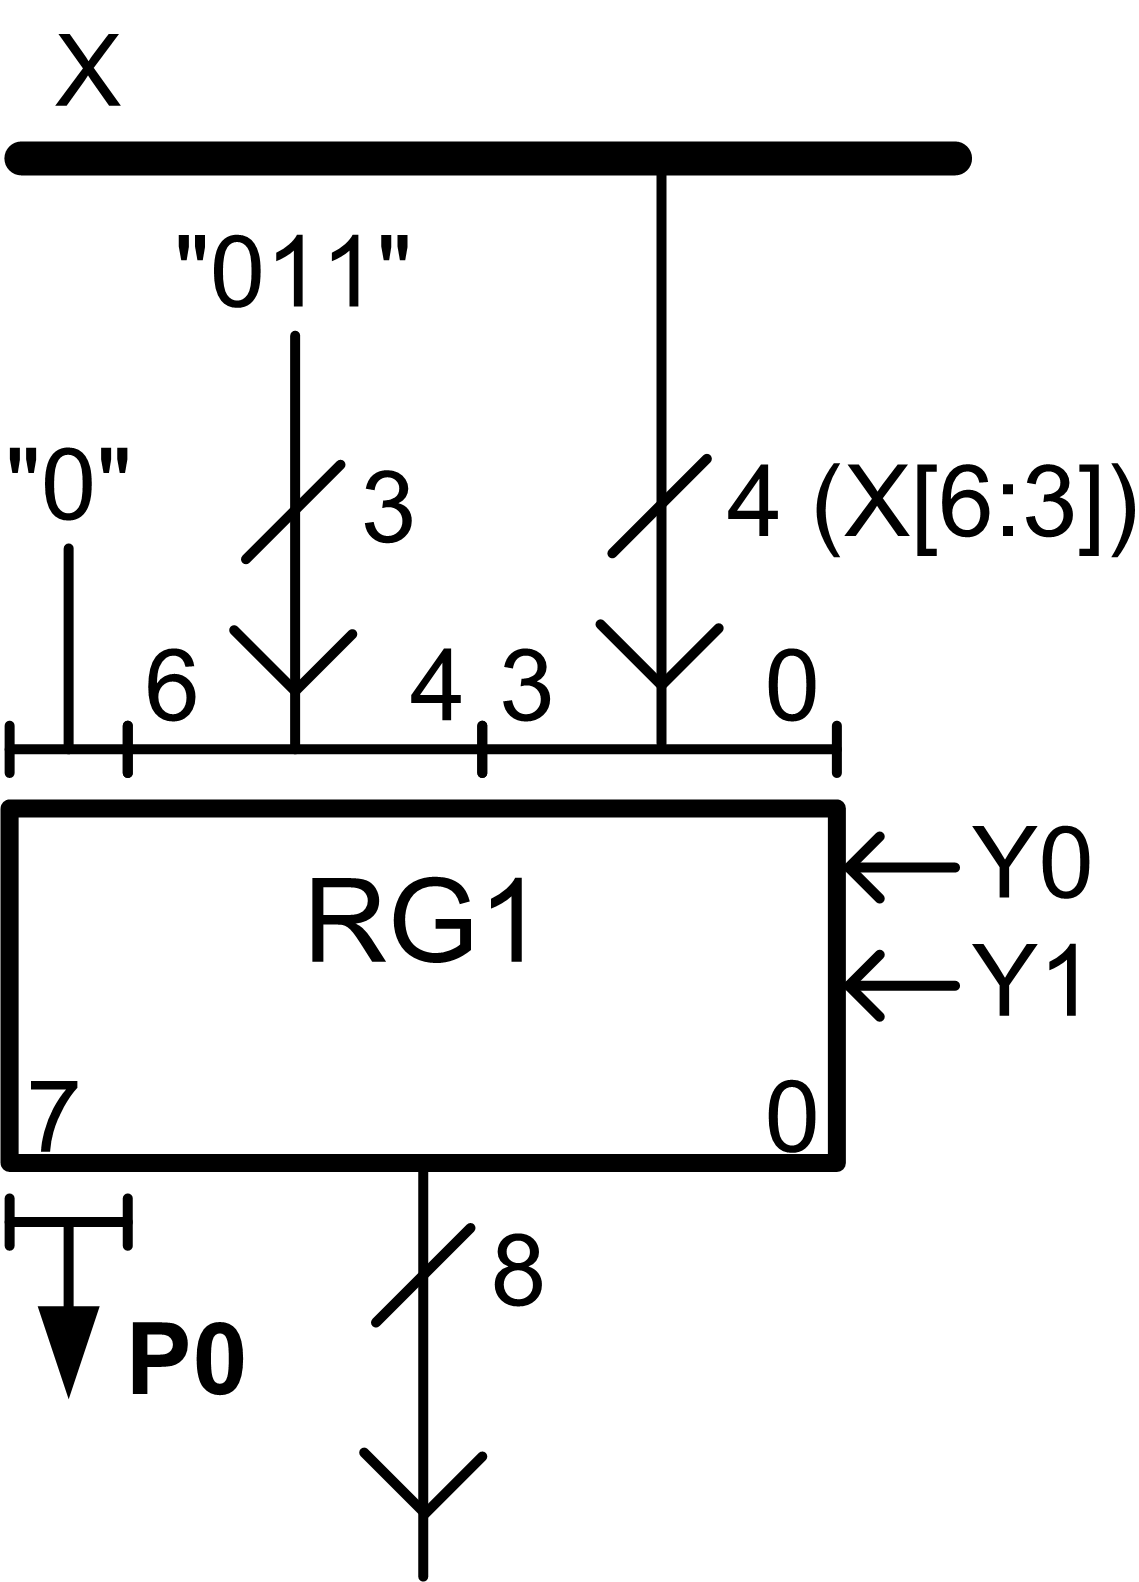
\includegraphics{fig/controls}
    \caption{Входы, выходы и управляющие сигналы регистра}
    \label{fig::ch::practice::controls}
\end{figure}

\begin{figure}[!ht]
    \centering
    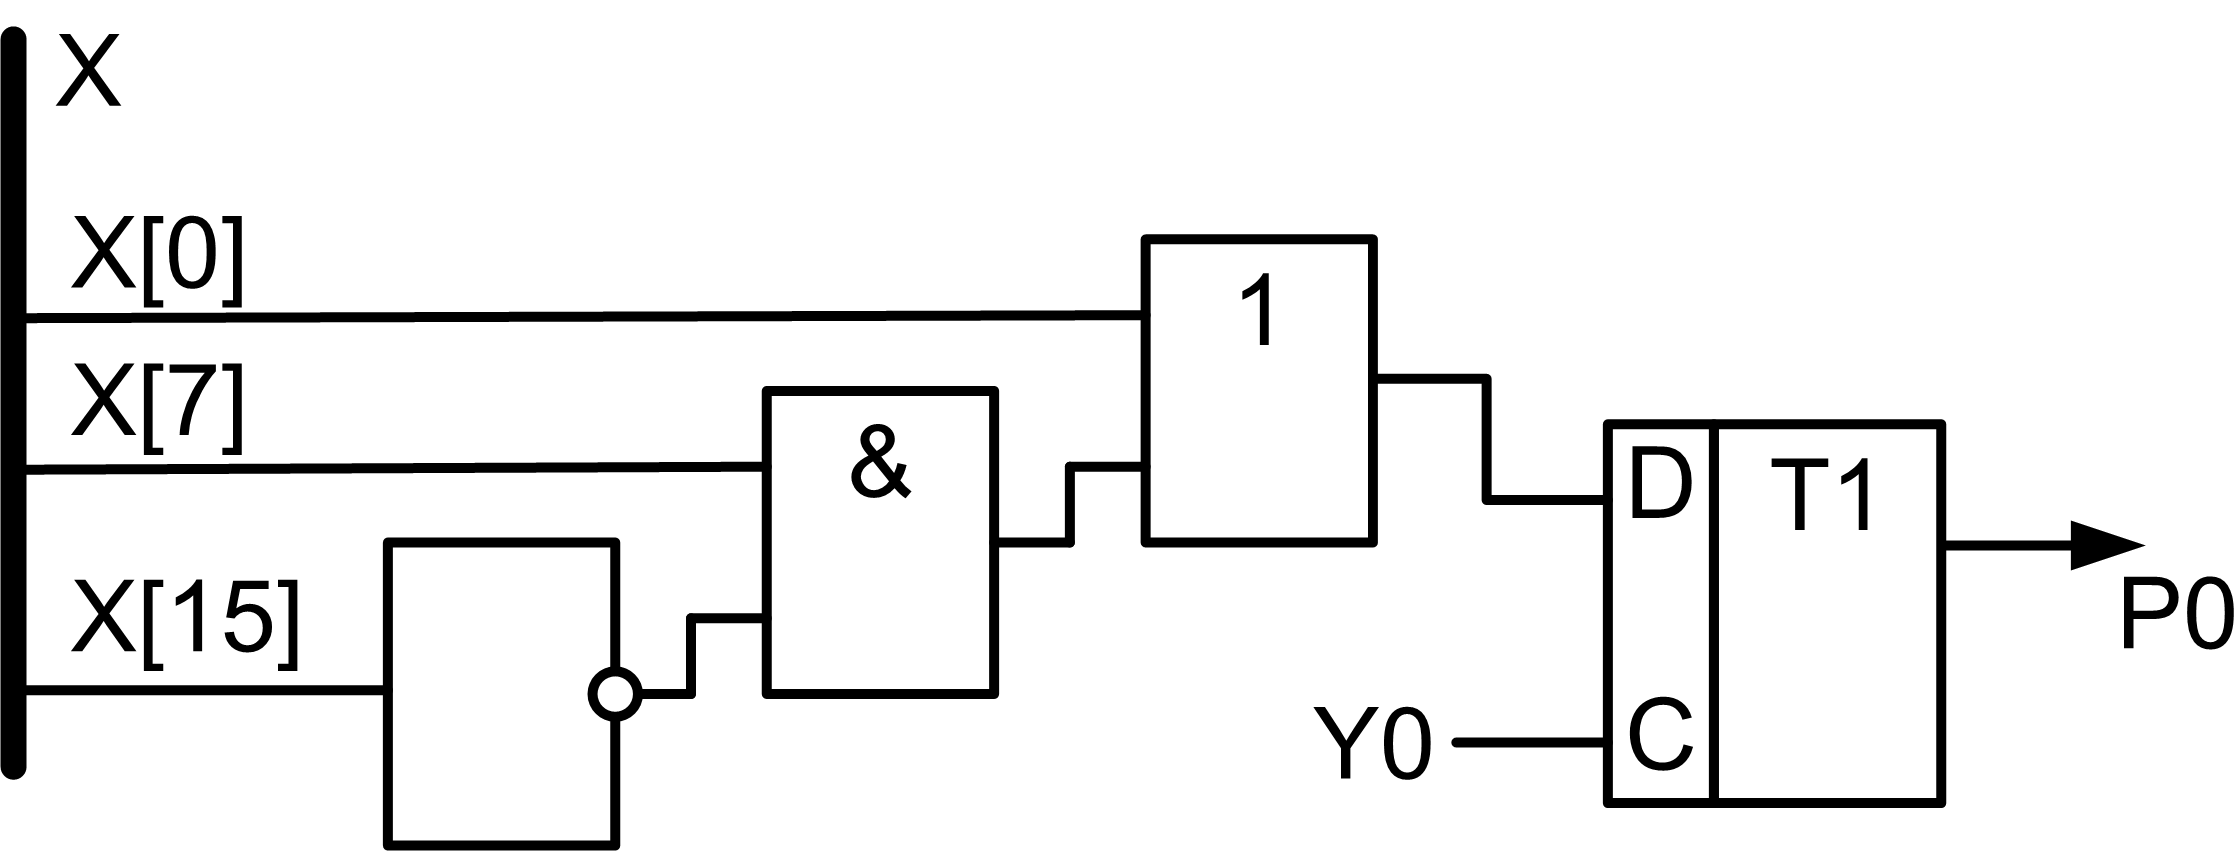
\includegraphics{fig/logic}
    \caption{Логическая схема}
    \label{fig::ch::practice::logic}
\end{figure}

Входы большинства элементов на схеме подводятся сверху, а выходы --- снизу. Исключением являются элементы логической схемы и триггеры (см. рисунок \ref{fig::ch::practice::logic}), в которой входы подаются слева, а выходы снимаются справа. В любом случае недопустимо разворачивать или переворачивать блоки.

Если о разрядности входов можно судить по разрядности выходов, то допустимо подписывать только разрядности выходов элементов.


\subsection{Элементы логики}

Элементы логики отличаются от элементов памяти тем, что представляют собой реализацию однотактной функции: выход формируется за один такт времени и зависит только от информации на входах. У элементов логики нет внутреннего состояния. Типичные элементы логики это: логические схемы (И, ИЛИ, НЕ, XOR, И-НЕ, и т.д.), мультиплексоры, сумматоры, шинные формирователи и т.д.


\subsubsection{Многовходовые логические функции}

На схемах элементы, реализующие многовходовую ассоциативную и комутативную логическую функцию (И, ИЛИ, XOR), допустимо изображать одним элементом, как на рисунке \ref{fig::ch::practice::bigLogic}.
\begin{figure}[!ht]
    \centering
    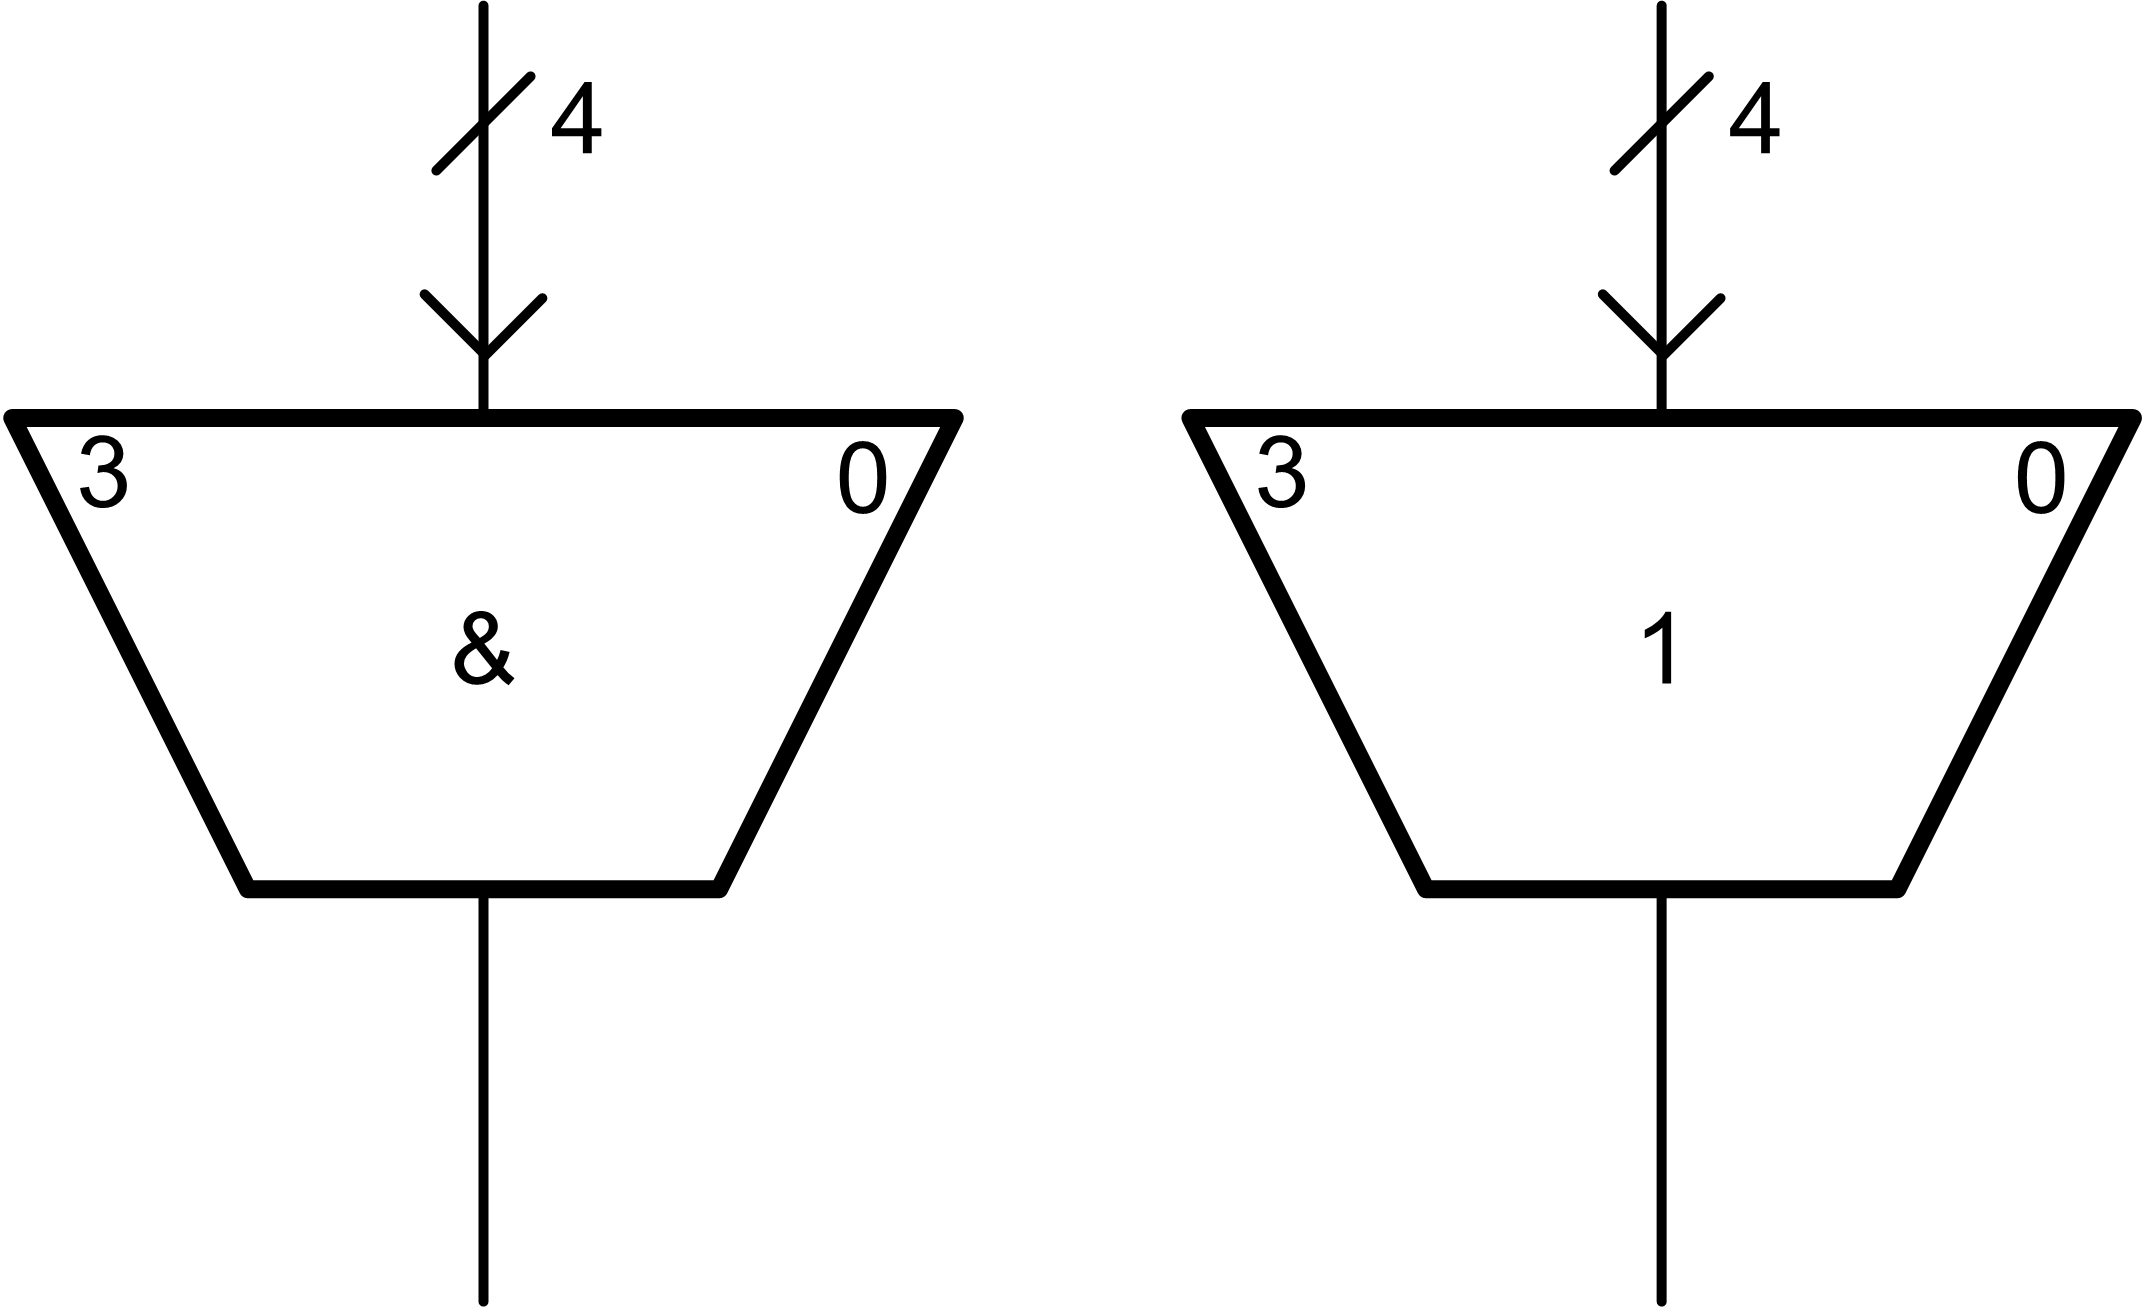
\includegraphics{fig/bigLogic}
    \caption{$4$-х входовые функции И, ИЛИ}
    \label{fig::ch::practice::bigLogic}
\end{figure}

Выход такого элемента --- одноразрядный.


\subsubsection{Инвертор}

На схемах многоразрядный инвертор изображается как рисунке \ref{fig::ch::practice::invertor}.
\begin{figure}[!ht]
    \centering
    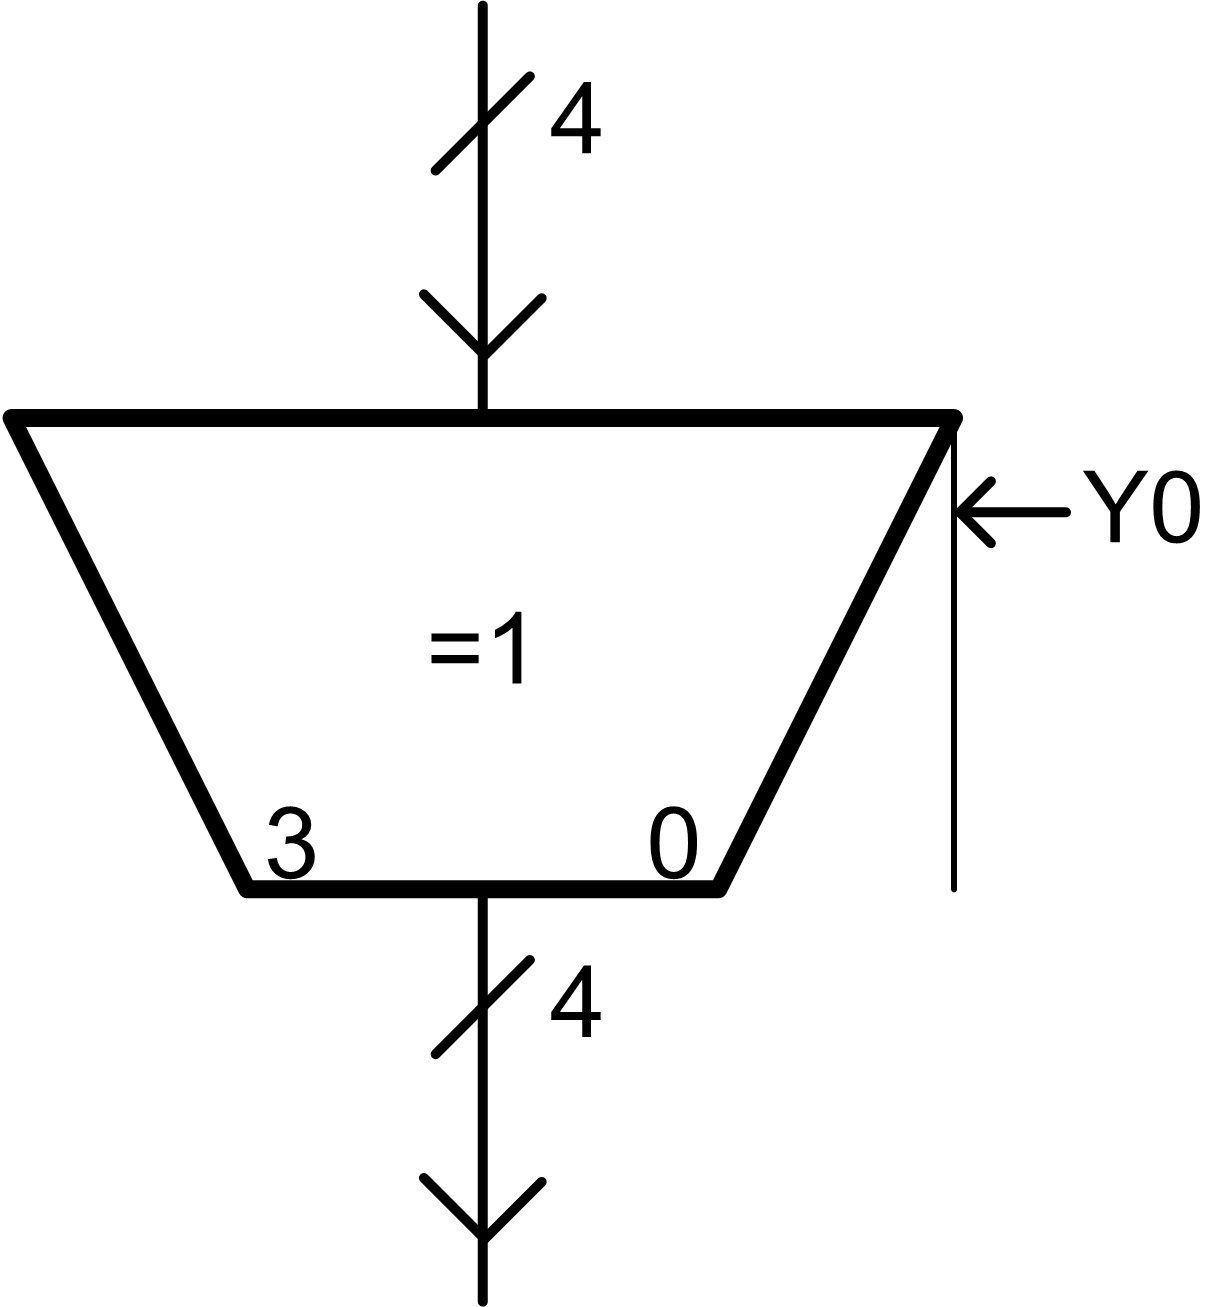
\includegraphics{fig/invertor}
    \caption{$4$-х разрядный инвертор}
    \label{fig::ch::practice::invertor}
\end{figure}

Если значение единственного управляющего сигнала 0, то разряды входа без изменений подаются на выход, иначе на выходе формируется поразрядная инверсия входа.

\subsubsection{Мультиплексор}

Условное графическое обозначение мультиплексора приведено на рисунке \ref{fig::ch::practice::mux}.
\begin{figure}[!ht]
    \centering
    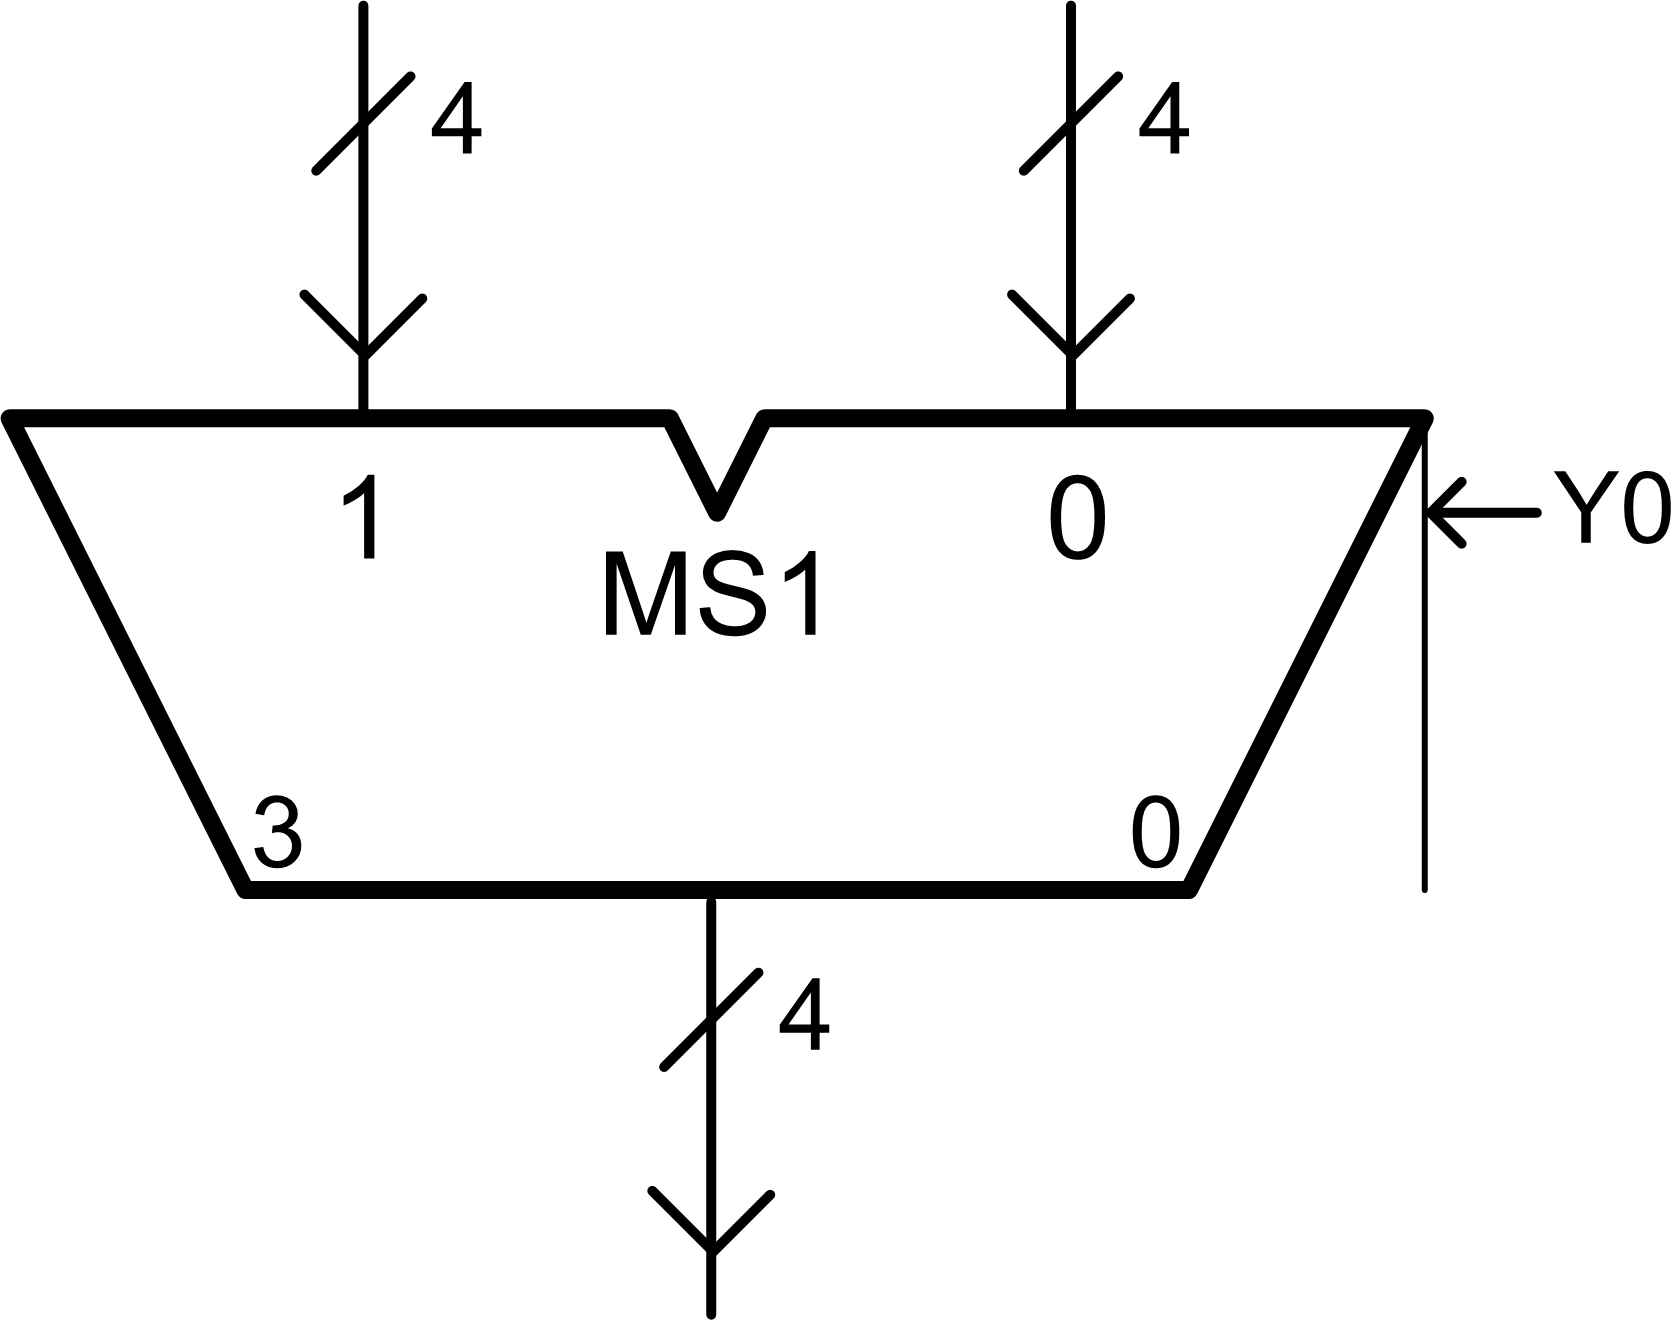
\includegraphics{fig/mux}
    \caption{Мультиплексор}
    \label{fig::ch::practice::mux}
\end{figure}

В зависимости от значения управляющего сиграла (на рисунке \ref{fig::ch::practice::mux} это $Y0$) на выход подается либо нулевое, либо первое входное плечо.

Мультиплексоры с большим количеством плеч могут быть получены на основе $2$-плечевых мультиплексоров каскадным подключением. Мультиплексор с произвольным количеством плеч рисуют упрощенно (см. рисунок \ref{fig::ch::practice::muxbig}). При этом самый верхний управляющий сигнал соответствует младшему разряду (LSB\footnote{LSB --- Least Significant Bit, Младший бит}) двоичного представления номера плеча, а самый нижний - старшему (MSB\footnote{MSB --- Most Significant Bit, Старший бит}). Например, чтобы выбрать 2-е плечо мультиплексора на рисунке \ref{fig::ch::practice::muxbig} нужно подать $Y1=1$, $Y0=0$.

\begin{figure}[!ht]
    \centering
    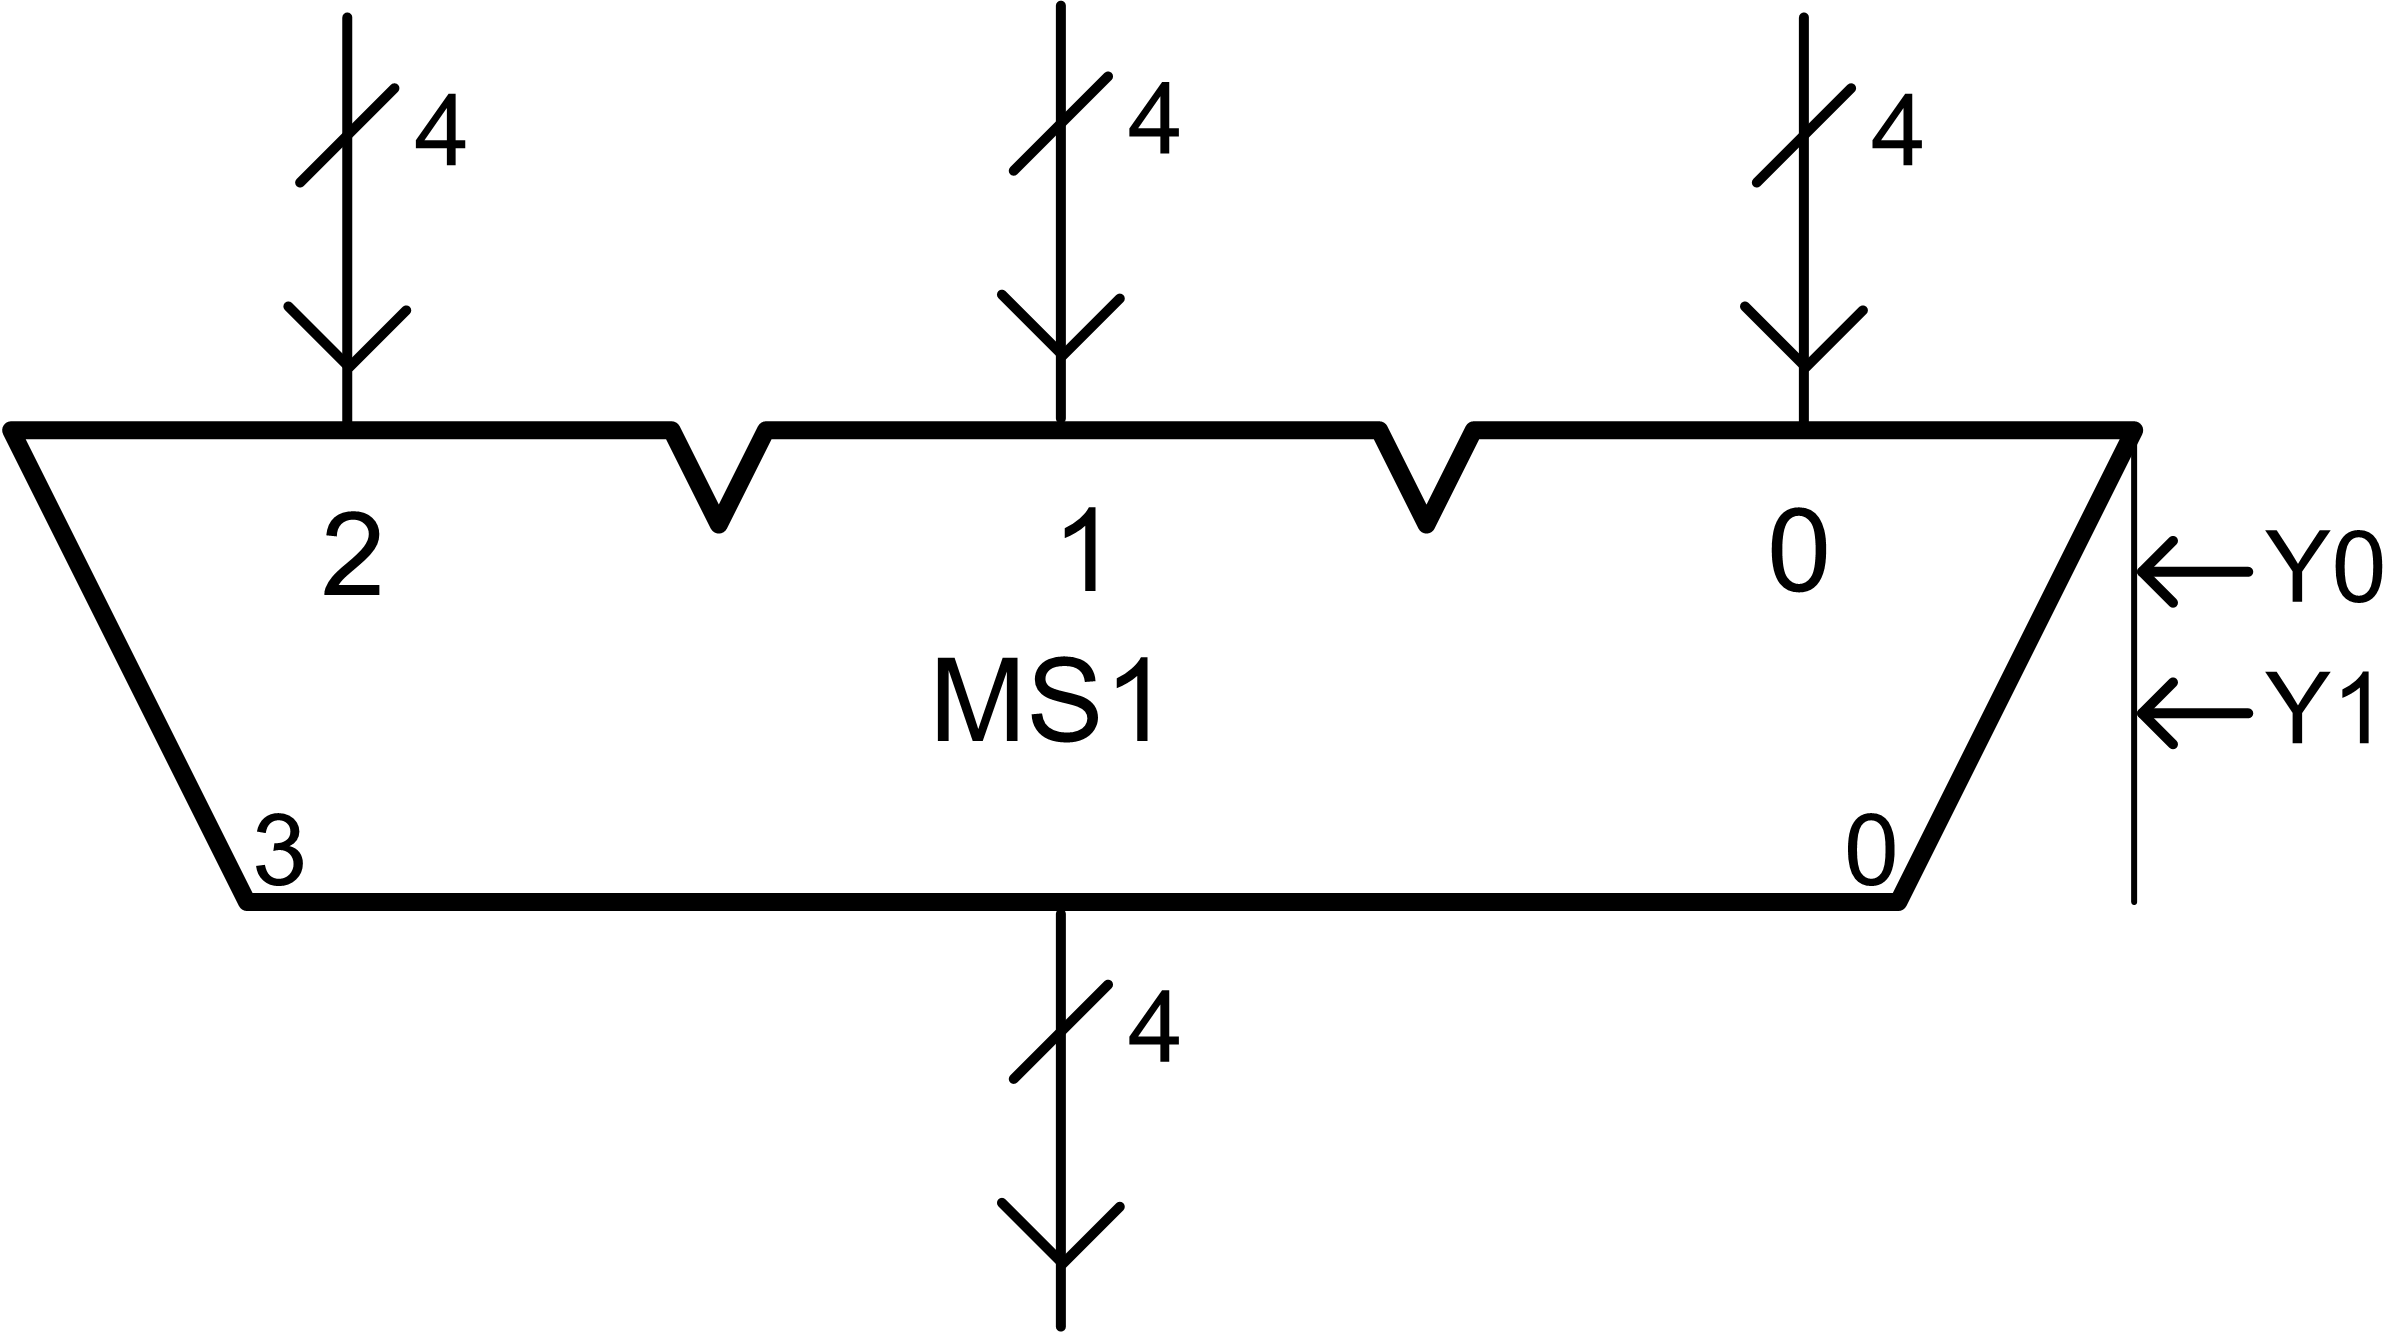
\includegraphics{fig/muxbig}
    \caption{Многоплечевой мультиплексор}
    \label{fig::ch::practice::muxbig}
\end{figure}


\subsubsection{Сумматор}

Условное графическое обозначение сумматора приведено на рисунке \ref{fig::ch::practice::summator}.
\begin{figure}[!ht]
    \centering
    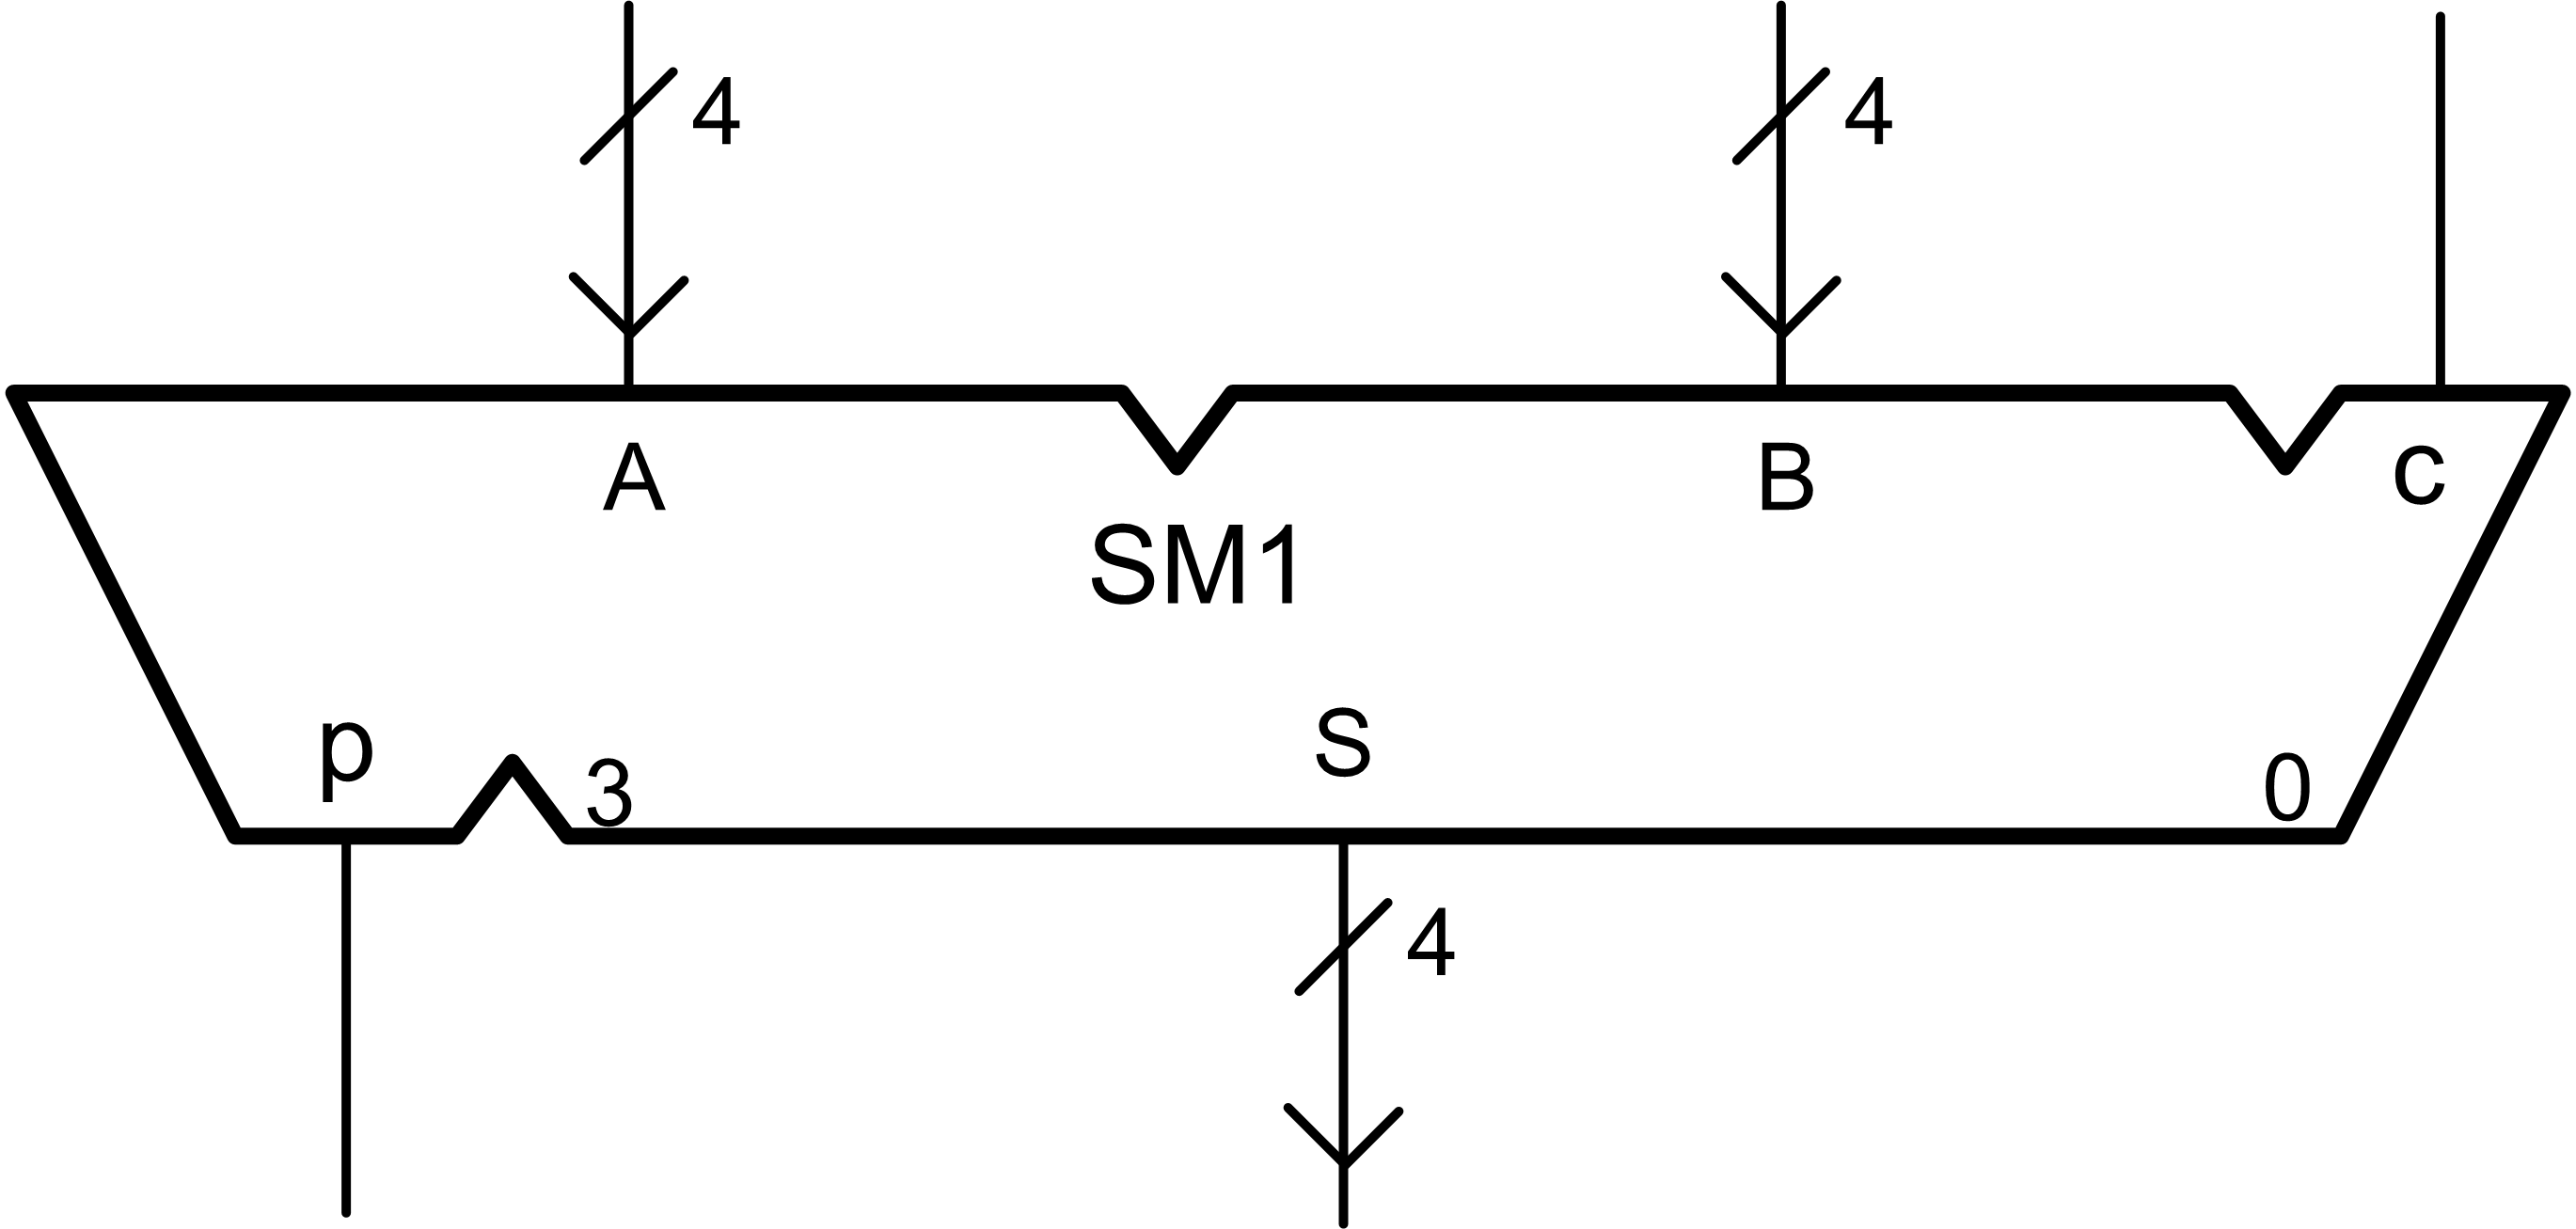
\includegraphics{fig/summator}
    \caption{Сумматор}
    \label{fig::ch::practice::summator}
\end{figure}

Сумматор выполняет арифметическое сложение $n$-разрядных входов (на рисунке \ref{fig::ch::practice::summator} $n=4$) входов $A$ и $B$ а также одноразрядного входа переноса в младшие разряды $c$. На выход $S$ выдаются младшие $n$ разрядов результата, а на выход $p$ --- бит переноса из старшего $(n-1)$-го разряда суммы $S$:
\begin{align*}
    S \equiv (A + B + c) \pmod{2^n};\\
    p = (A + B + c) \div{2^n}.
\end{align*}

В случае, если нужно получить сумматор большей разрядности на основе сумматоров меньшей разрядности, то выход переноса из старших разрядов младшего сумматора замыкают на вход переноса старшего сумматора (см. рисунок \ref{fig::ch::practice::summators}).
\begin{figure}[!ht]
    \centering
    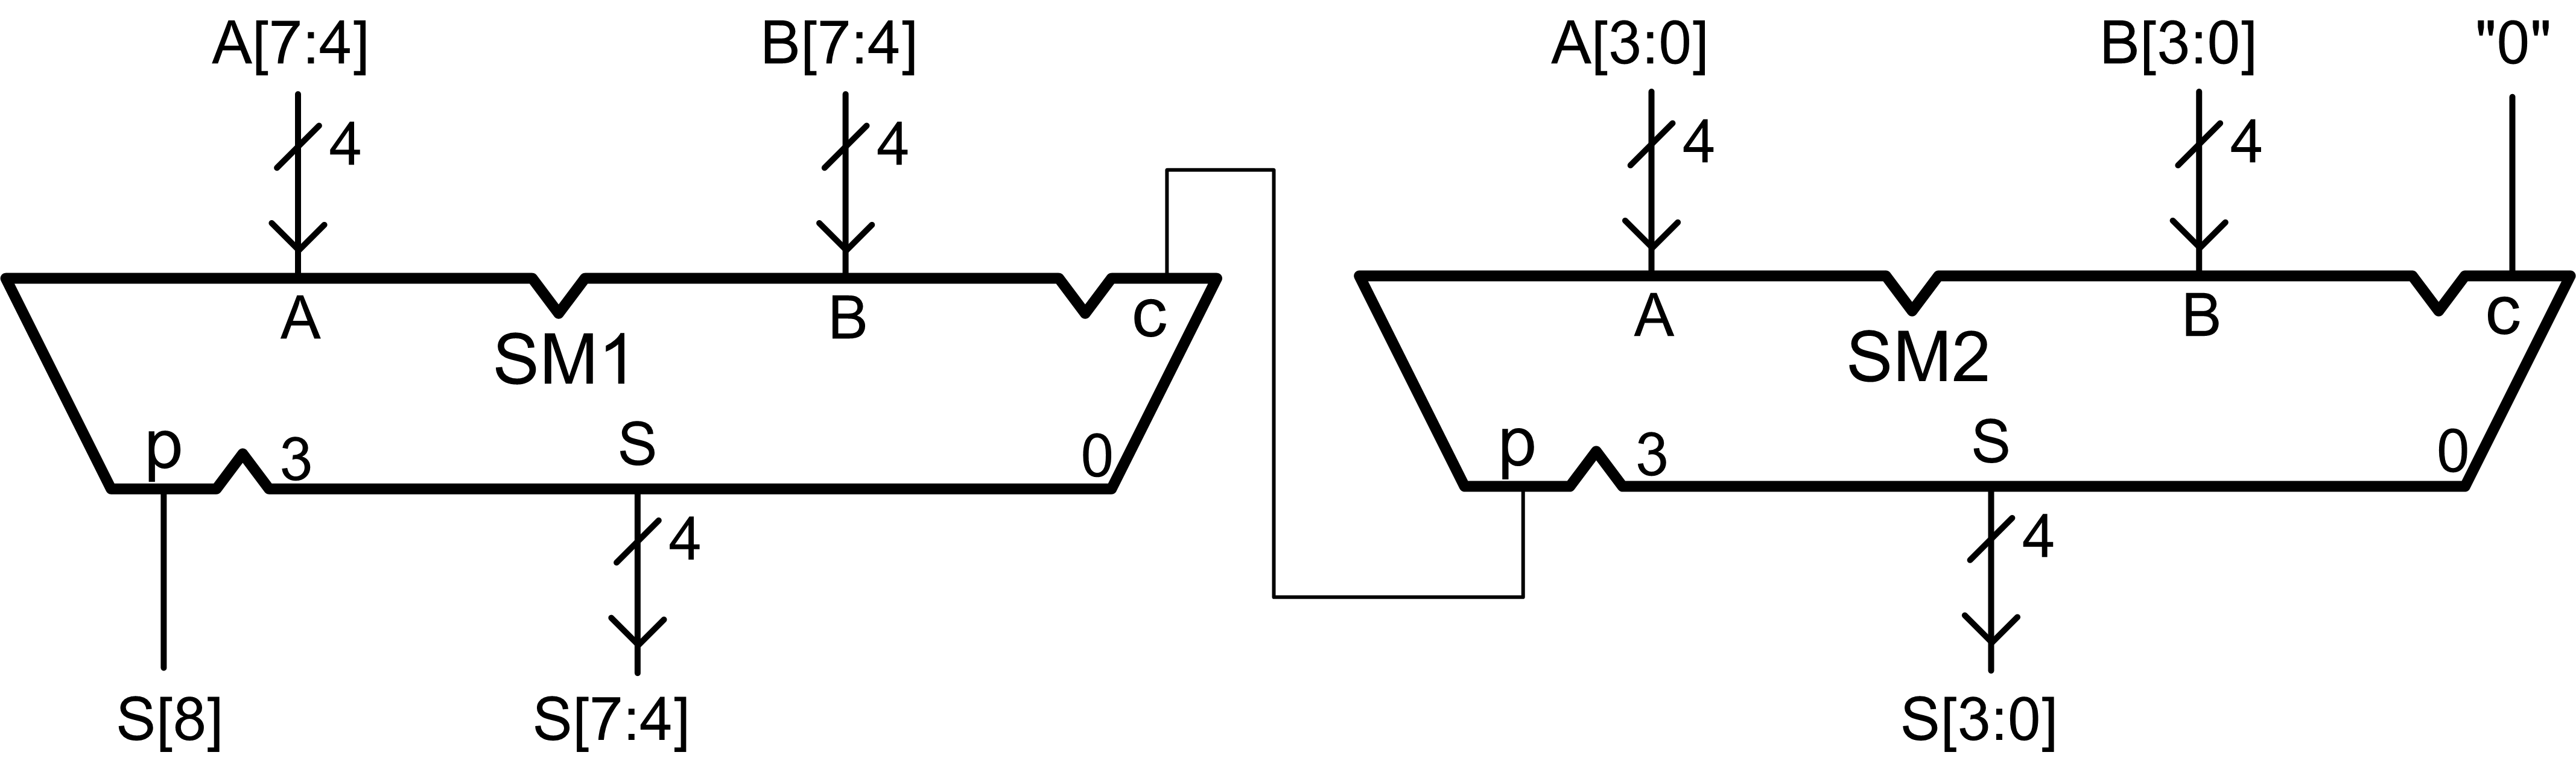
\includegraphics[width=.85\textwidth]{fig/summators}
    \caption{8-разрядный сумматор на основе двух 4-х разрядных}
    \label{fig::ch::practice::summators}
\end{figure}

На схемах сумматор любой разрядности рисуют одним элементом, если неважно, как этот сумматор устроен.


\subsubsection{Шинный формирователь}

Шинным формирователем устройство называется потому, что обычно его выходы подключены к шине. По управляюещму сигналу (на рисунке \ref{fig::ch::practice::zbuffer} сигнал $Y0$) шинный формирователь может отключать свои выходы от шины. Когда шинный формирователь подключен к шине, он выдает данные со входа на шину. Так как шина может быть общей для нескольких устройств, то использование шинных формирователей обязательно, чтобы гарантировать, что только одно устройство выдает на шину данные.

\begin{figure}[!ht]
    \centering
    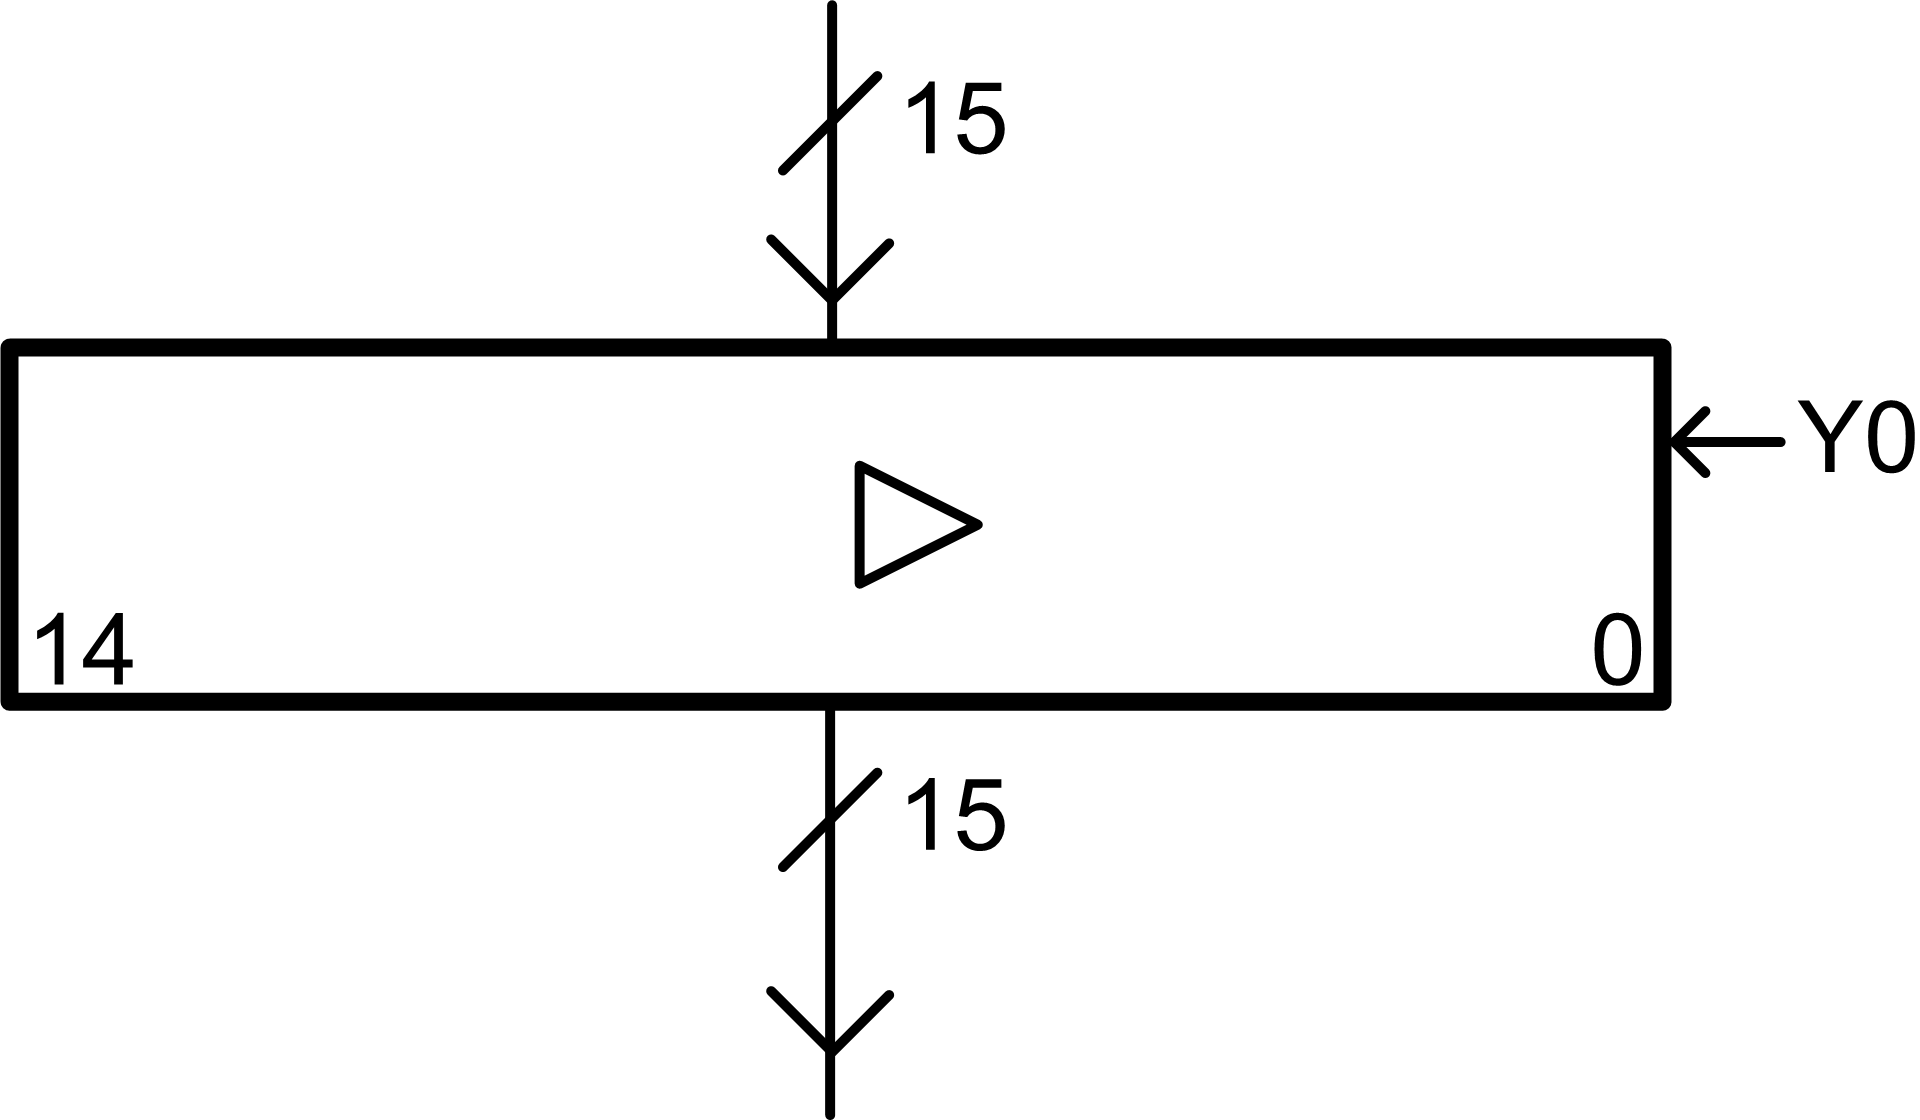
\includegraphics{fig/zbuffer}
    \caption{15-разрядный шинный формирователь}
    \label{fig::ch::practice::zbuffer}
\end{figure}


\subsection{Элементы памяти}

Элементы памяти могут сохрянять информацию (состояние) между тактами. Они обычно имеют управляющий сигнал, который управляет запоминанием информации со входов. Т.е. в течение такта такой элемент либо <<запоминает>> информацию со входов, либо хранит (или преобразует) ранее запомненную информацию.

\subsubsection{Регистры}
\label{sss::ch::practice::regiter}

Обычный регистр содержит автономную $n$-разрядную ячейку памяти и предназначен только для запоминания $n$ бит информации со входов. Помимо основной функции он может, например, выполнить сброс всех бит своей ячейки памяти в $0$ или $1$. На выходы регистра всегда выдается содержимое его внутренней ячейки памяти.

\begin{figure}[!ht]
    \centering
    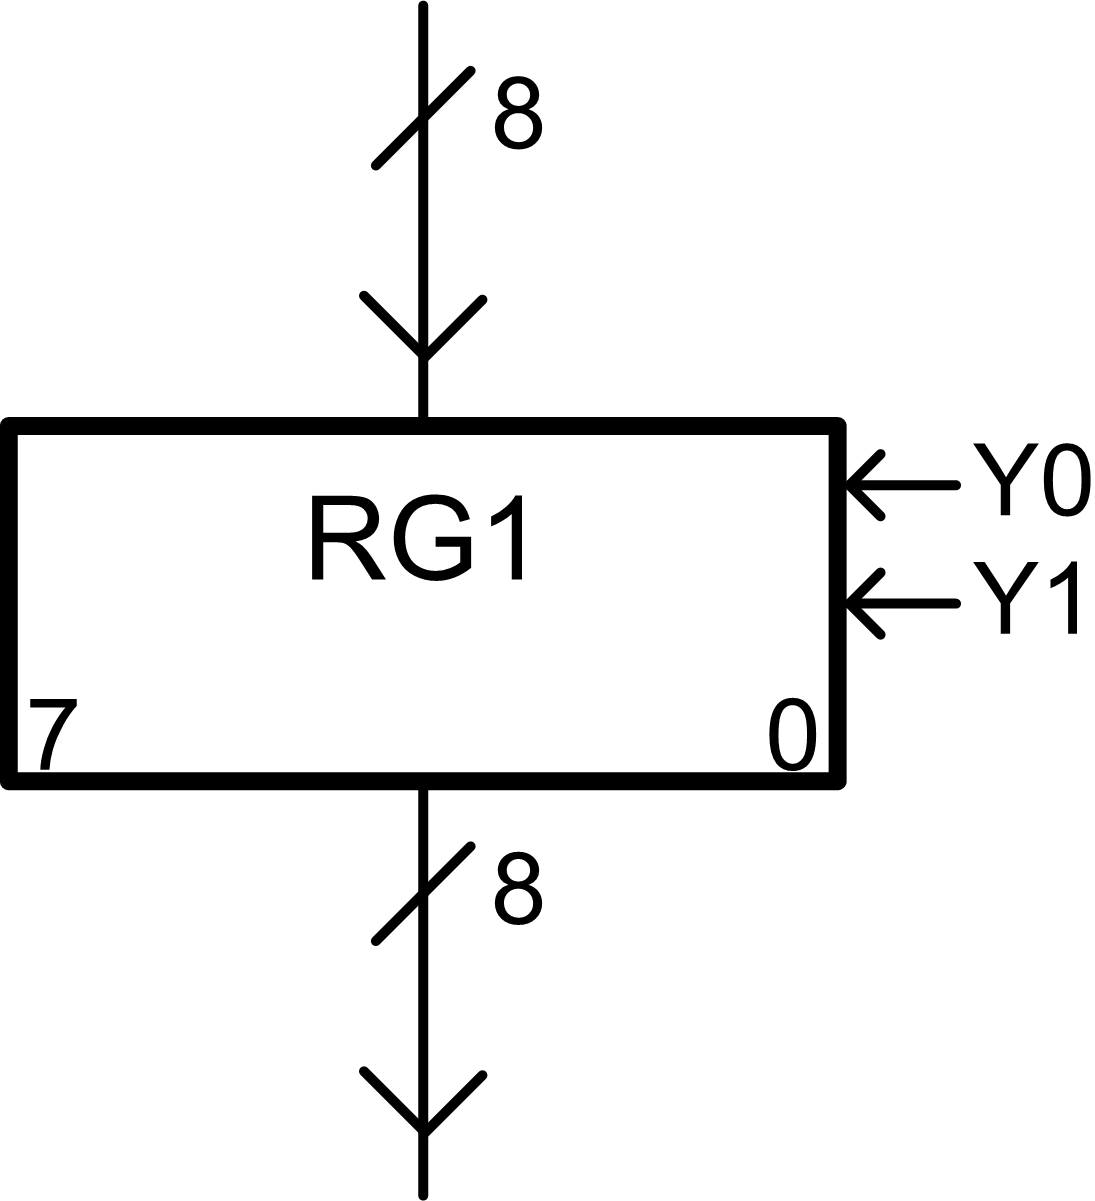
\includegraphics{fig/register}
    \caption{8-разрядный регистр}
    \label{fig::ch::practice::register}
\end{figure}

Например, на рисунке \ref{fig::ch::practice::register} изображен обычный регистр, расшифровка управляющих сигналов которого может быть следующей:
\begin{itemize}
    \item $Y0$ --- разрешение записи в $RG1$. Если данный сигнал подается в течение такта, то регистр <<запоминает>> информацию со входов и хранит до тех пор, пока $Y0$ вновь не будет подан в будущем.

    \item $Y1$ --- сброс всех разрядов внутренней ячейки памяти $RG1$ в $0$.
\end{itemize}

Управляющие сигналы регистра могут конфликтовать, например, состояние регистра не определено, если одновременно подать сигналы разрешения записи и сброса.

Сдвиговые регистры изображаются особым образом, в виде параллелограмма. Направление сдвига разрядов ячейки памяти обозначается стрелкой внутри регистра. Например, при сдвиге влево значение старшего разряда теряется, а в младший разряд заносится значение разряда со специального входа, который изображается боковой планкой с нужного края. 

\begin{figure}[!ht]
    \centering
    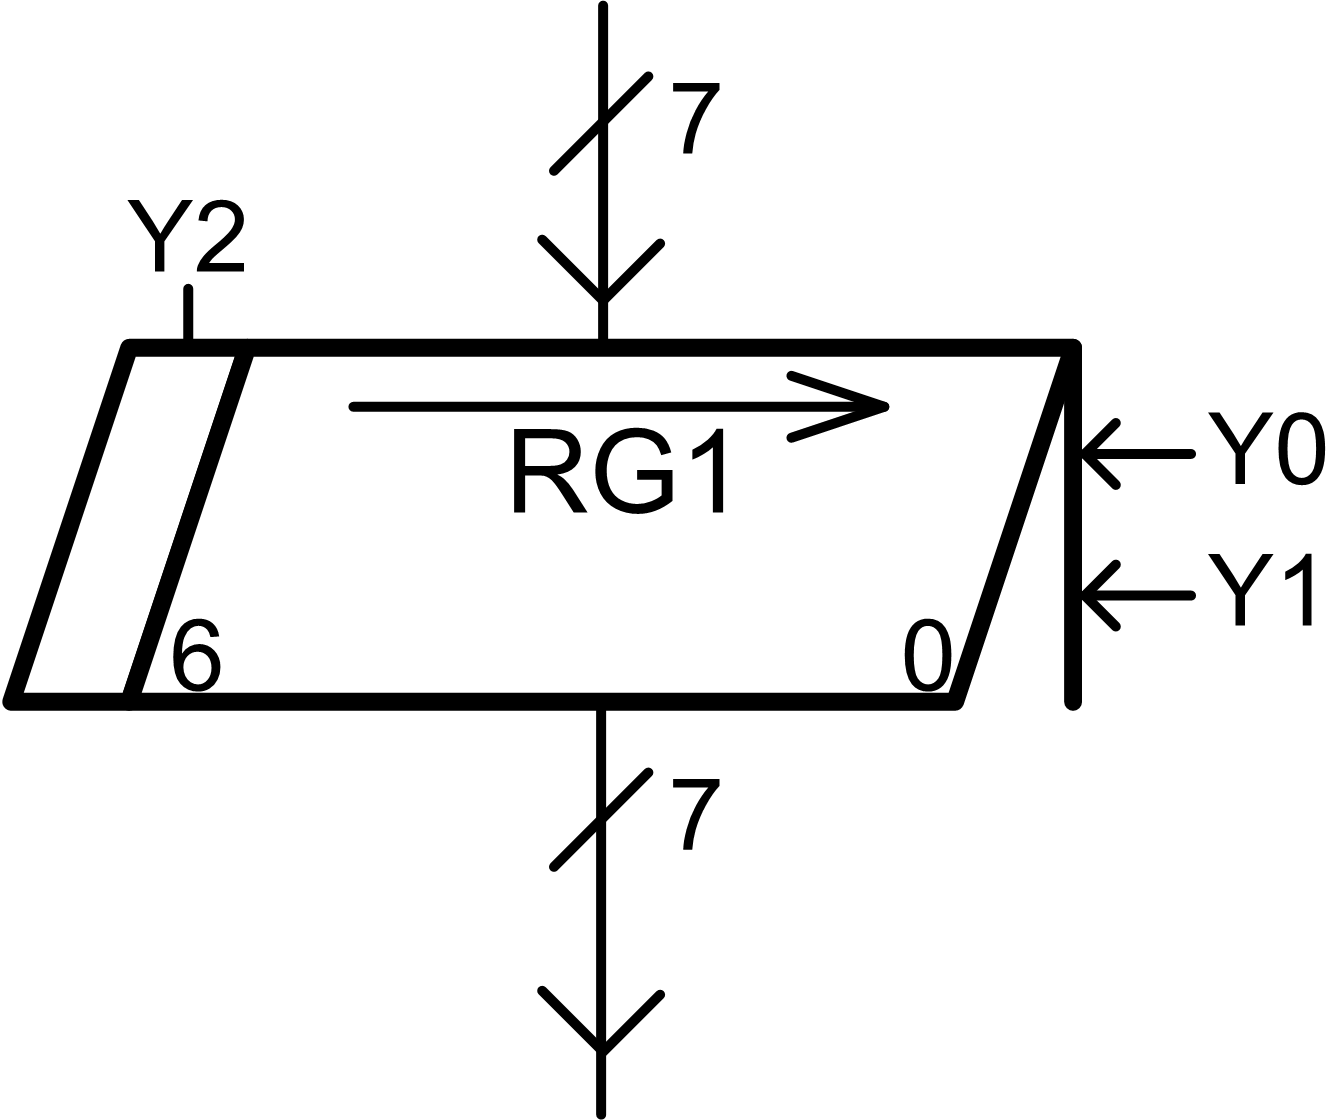
\includegraphics{fig/shiftregister}
    \caption{7-разрядный сдвиговый регистр}
    \label{fig::ch::practice::shiftregister}
\end{figure}

На рисунке \ref{fig::ch::practice::shiftregister} изображен сдвиговый регистр, расшифровка управляющих сигналов которого может быть следующей:
\begin{itemize}
    \item $Y0$ --- разрешение записи в $RG1$. Если данный сигнал подается в течение такта, то регистр <<запоминает>> информацию со входов и хранит до тех пор, пока $Y0$ вновь не будет подан в будущем.

    \item $Y1$ --- сдвиг $RG1$ вправо.
    
    \item вход $Y2$ определяет значение $6$-го разряда при сдвиге.
\end{itemize}


\subsubsection{Триггеры}

Триггер --- это одноразрядное запоминающее устройство. Триггеров существует несколько видов: D, RS, JK, \ldots В схемах будет использоваться D-триггер (см. рисунок \ref{fig::ch::practice::dtrigger}), который можно считать одноразрядным регистром: если на вход $C$ подается 1, то триггер <<запоминает>> бит информации со входа $D$, а если на вход $C$ подается 0, то триггер выдает ранее запомненный бит.

\begin{figure}[!ht]
    \centering
    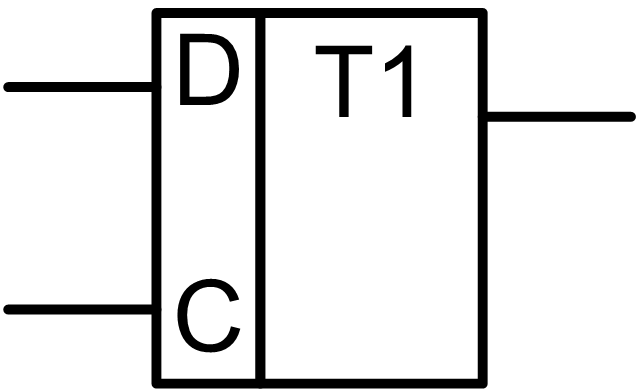
\includegraphics{fig/dtrigger}
    \caption{D-триггер}
    \label{fig::ch::practice::dtrigger}
\end{figure}

\section{Основы микропрограммного управления}
\label{ch::practice::programming}

Множительное устройство, ЦУУ и другие модули (см. рисунок \ref{fig::ch::practice::model}) работают автономно и каждый выполняет собственный алгоритм функционирования. Например, УЧ множительного устройства в бесконечном цикле выполняет алгоритм: принять задания от ЦУУ; выполнить умножение; выдать в ЦУУ результаты. ЦУУ, например, выполняет в бесконечном цикле алгоритм: считать очередную команду программы пользвателя из памяти; декодировать её; выдать необходимые задания исполнительным модулям; дождаться результатов, считать и сохранить их; выбрать следующую команду\ldots

УЧ модуля (в том числе и множительного устройства) представляет собой автомат, по тактам выполняющий алгоритм работы модуля. Существует несколько способов создания таких автоматов. В данном разделе будут рассморены математические основы функционирования управляющих автоматов, а затем особый вид таких автоматов --- \emph{микропрограммные}.

В математической основе выделяют два типа управляющих автоматов: автоматы Мили и автоматы Мура. Общим для автоматов обоих типов является:
\begin{itemize}
    \item Внутреннее состояние. Автомат в течение такта находится в одном из множества возможных внутренних состояний. По завершении такта, автомат переключается в новое состояние. Множество внутренних состояний 
    \[ 
        S=\{s_0,\ldots,s_{n-1}\}.
    \]
    
    \item Начальное состояние $s_0$. С этого внутреннего состояния автомат начинает свою работу.
    
    \item Набор значений (вектор) осведомительных сигналов
    \[
        P=(p_{m-1},\ldots,p_0).
    \]
	
	Новое внутреннее состояние, в которое перейдет автомат, определяется его текущим внутренним состоянием и значениями осведомительных сигналов, которые поступали ему в течение такта.
    
    
    \item Набор управляющих сигналов
    \[
        Y=(y_{k-1},\ldots,y_0).
    \]
	
	Автомат в течение такта формирует и выдает значения управляющих сигналов. В способе формирования  управляющих сигналов заключается главное отличие между автоматами Мили и Мура.
\end{itemize}

Если в $i$-м такте автомат находится в состоянии $s^{(i)}$, и поступают значения осведомительных сигналов $P^{(i)}$, то состояние $s^{(i+1)}$, в которое он перейдет в следующем такте, определяется функцией перехдов $\mathbf{S}$, а набор управляющих сигналов, которые выдаются в $i$-м такте $Y^{(i)}$ определяются функцией выходов $\mathbf{Y}$.

Для автомата Мили:
\begin{equation}
    \begin{aligned}
        s^{(i+1)}&=\mathbf{S}(s^{(i)}, P^{(i)});\\
        Y^{(i)}  &=\mathbf{Y}(s^{(i)}, P^{(i)}).
    \end{aligned}
    \label{eq::ch::practice::programming::Mili}
\end{equation}

Видно, что для автомата Мили векор управляющих сигналов $Y^{(i)}$ формируется на основе текущего состояния $s^{(i)}$ и вектора осведомительных сигналов $P^{(i)}$.

Для автомата Мура управляющие сигналы зависят только от текущего состояния:
\begin{equation}
    \begin{aligned}
        s^{(i+1)}&=\mathbf{S}(s^{(i)}, P^{(i)});\\
        Y^{(i)}  &=\mathbf{Y}(s^{(i)}).
    \end{aligned}
    \label{eq::ch::practice::programming::Moore}
\end{equation}

Работу автомата удобно изобразить на диаграмме переходов, которая представляет собой граф, вершинам которого соответствуют состояния, а дугам --- функция переходов $\mathbf{S}$. Начальное состояние $s_0$ обычно выделяется двойным контуром. Над дугой подписываются значения осведомительных сигналов, определяющих переход в следующее состояние. Так как управляющие сигналы в автомате Мили зависят от состояния автомата и осведомительных сигналов, то управляющими сигналами взвешиваются дуги. В автомате Мура управляющие сигналы зависят только от состояния, поэтому управляющими сигналами взвешиваются вершины.

Далее приводятся примеры диаграмм переходов автоматов, из раздела \ref{ss::ch::practice::software::example}, к этому разделу следует обратиться всем желающим понять назначение управляющих и осведомительных сигналов. Пока же --- это неважно.

\begin{figure}[!ht]
    \[
        {\xymatrix{
            *{}
                &*{}
                    &*{}
                        &s_3  \ar@{->}@/^/[dr]^(.3){*|\Machine{22h}} 
                            &*{}
                                &*{}
                                    &*{}
                                        &*{}
                                            \\
            *++[o][F=]{s_0}  \ar@{->}[r]^{p_0|\Machine{1h}}  \ar@{->}@(ur,ul)[]_{\bar{p}_0|\Machine{1h}}
                &s_1  \ar@{->}[r]^{*|\Machine{4h}}
                    &s_2  \ar@{->}[rr]^{\bar{p}_2|\Machine{12h}} \ar@{->}@/^/[ur]^{p_2|\Machine{18h}}
                        &*{}
                            &s_4  \ar@{->}[rr]^{p_1|\Machine{2h}} \ar@{->}@(r,u)[]_(.6){\bar{p}_1|\Machine{2h}}
                                &*{}
                                    &s_5  \ar@{->}@(d,d)[llllll]_{*|\Machine{41h}}
        }}
    \]
    \caption{Диаграмма переходов автомата Мили}
    \label{fig::ch::practice::MiliDiagram}
\end{figure}

На рисунке \ref{fig::ch::practice::MiliDiagram} приведена диаграмма автомата Мили. Далее приводится описание нескольких переходов.
\begin{itemize}
    \item Из начального состояния $s_0$, автомат переходит в состояние $s_1$, при $p_0=1$ (на схеме это обозначено как $p_0$); при этом выдается управляющий сигнал $y_0$ (на схеме вектор управляющих сигналов закодирован в 16-ичной СС: \Machine{1h}).
    
    \item Автомат остается в начальном состояниии если $\bar{p}_0$, при этом также выдается $y_0$.

    \item Из $s_1$ осуществляется переход только в $s_2$ --- осведомительные сигналы не важны (переход помечен $*$), при этом выдается управляющий сигнал $y_2$ (вектор \Machine{4h}).
    
    \item Из $s_5$ автомат безусловно возвращается в $s_0$ и выдает при этом набор сигналов $\{y_6,y_0\}$, т.е. вектор \Machine{41h}.
\end{itemize}

Из состояния $s_1$ автомат переходит только в состояние $s_2$, при этом значения осведомительных сигналов не важны и обозначены на схеме $*$, выдается управляющий сигнал $y_0$. И т.д.

\begin{figure}[!ht]
    \[
        {\xymatrix{
            *{} &*{}&*{}&*{}&*{}&*{}&*{}    \\
            *{}
                &*{}
                    &*{}
                        &s_5|\Machine{10h}    \ar@{->}@/^/[rrd]^{*} 
                            &*{}
                                &*{}
                                    &*{}
                                        \\
            *++[o][F=]{s_0|\Machine{1h}}  \ar@{->}[r]^{p_0}  \ar@{->}@(ur,ul)[]_{\bar{p}_0}
                &s_1|\Machine{4h}  \ar@{->}[r]^{*}
                    &s_2|\Machine{0h}  \ar@{->}[r]^{p_2}  \ar@{->}@/^/[ru]^{\bar{p}_2}
                        &s_3|\Machine{18h}  \ar@{->}[r]^{*}
                            &s_4|\Machine{20h}  \ar@{->}[r]^{*}
                                &s_6|\Machine{2h}  \ar@{->}[r]^{p_1} \ar@{->}@(ur,ul)[]_{\bar{p}_1}
                                    &s_7|\Machine{41h} \ar`d[dl]`_u[llllll]_{\bar{p}_0}[llllll]
                                                       \ar`u[uul]`[lllll]_{p_0}[lllll]
                                        %\ar@{->}@(d,d)[llllll]_{\bar{p}_0} \ar@{->}@(u,u)[lllll]_{p_0}
                                            \\
            *{} &*{}&*{}&*{}&*{}&*{}&*{}    \\
        }}
    \]
    \caption{Диаграмма переходов автомата Мура}
    \label{fig::ch::practice::MooreDiagram}
\end{figure}

На рисунке \ref{fig::ch::practice::MooreDiagram} приведена диаграмма автомата Мура. Далее следует описания нескольких переходов автомата.
\begin{itemize}
    \item Находясь в начальном состоянии, автомат выдает управлающий сигнал $y_0$ (вектор \Machine{1h}). Если выполняется условие $\bar{p}_0$, т.е. $p_0=0$, то автомат остается в начальном состоянии, в противном случае --- переходит в $s_1$.
    
    \item Из состояния $s_3$, в котором автомат выдает управляющие сигналы $\{y_4,y_3\}$, автомат безусловно переходит в $s_4$.
    
    \item Из состояния $s_5$ автомат может вернуться в начальное состояние или выполнить переход в $s_0$.
\end{itemize}

\emph{Микропрограммный} автомат в своем составе имеет два элемента --- микропроцессор и память \emph{микрокоманд}. Такие автоматы довольно удобны в обращении, так как позволяют задать алгоритм своей работы простой записью микропрограммы в память микрокоманд. Микрокоманда выполняется за один такт и сопровождается выдачей соответствующих управляющих сигналов.


\subsection{Микропрограммные автоматы}

Структура микропрограммного автомата Мили представлена на рисунке\footnote{Мы намеренно отступили от некоторых правил оформления схем --- например, мультиплексор MS1 в нашей схеме перевернут, а управление на MS2 подается слева} \ref{fig::ch::practice::Mili}, а Мура --- на рисунке \ref{fig::ch::practice::Moore}. 

\begin{figure}[!ht]
    \centering
    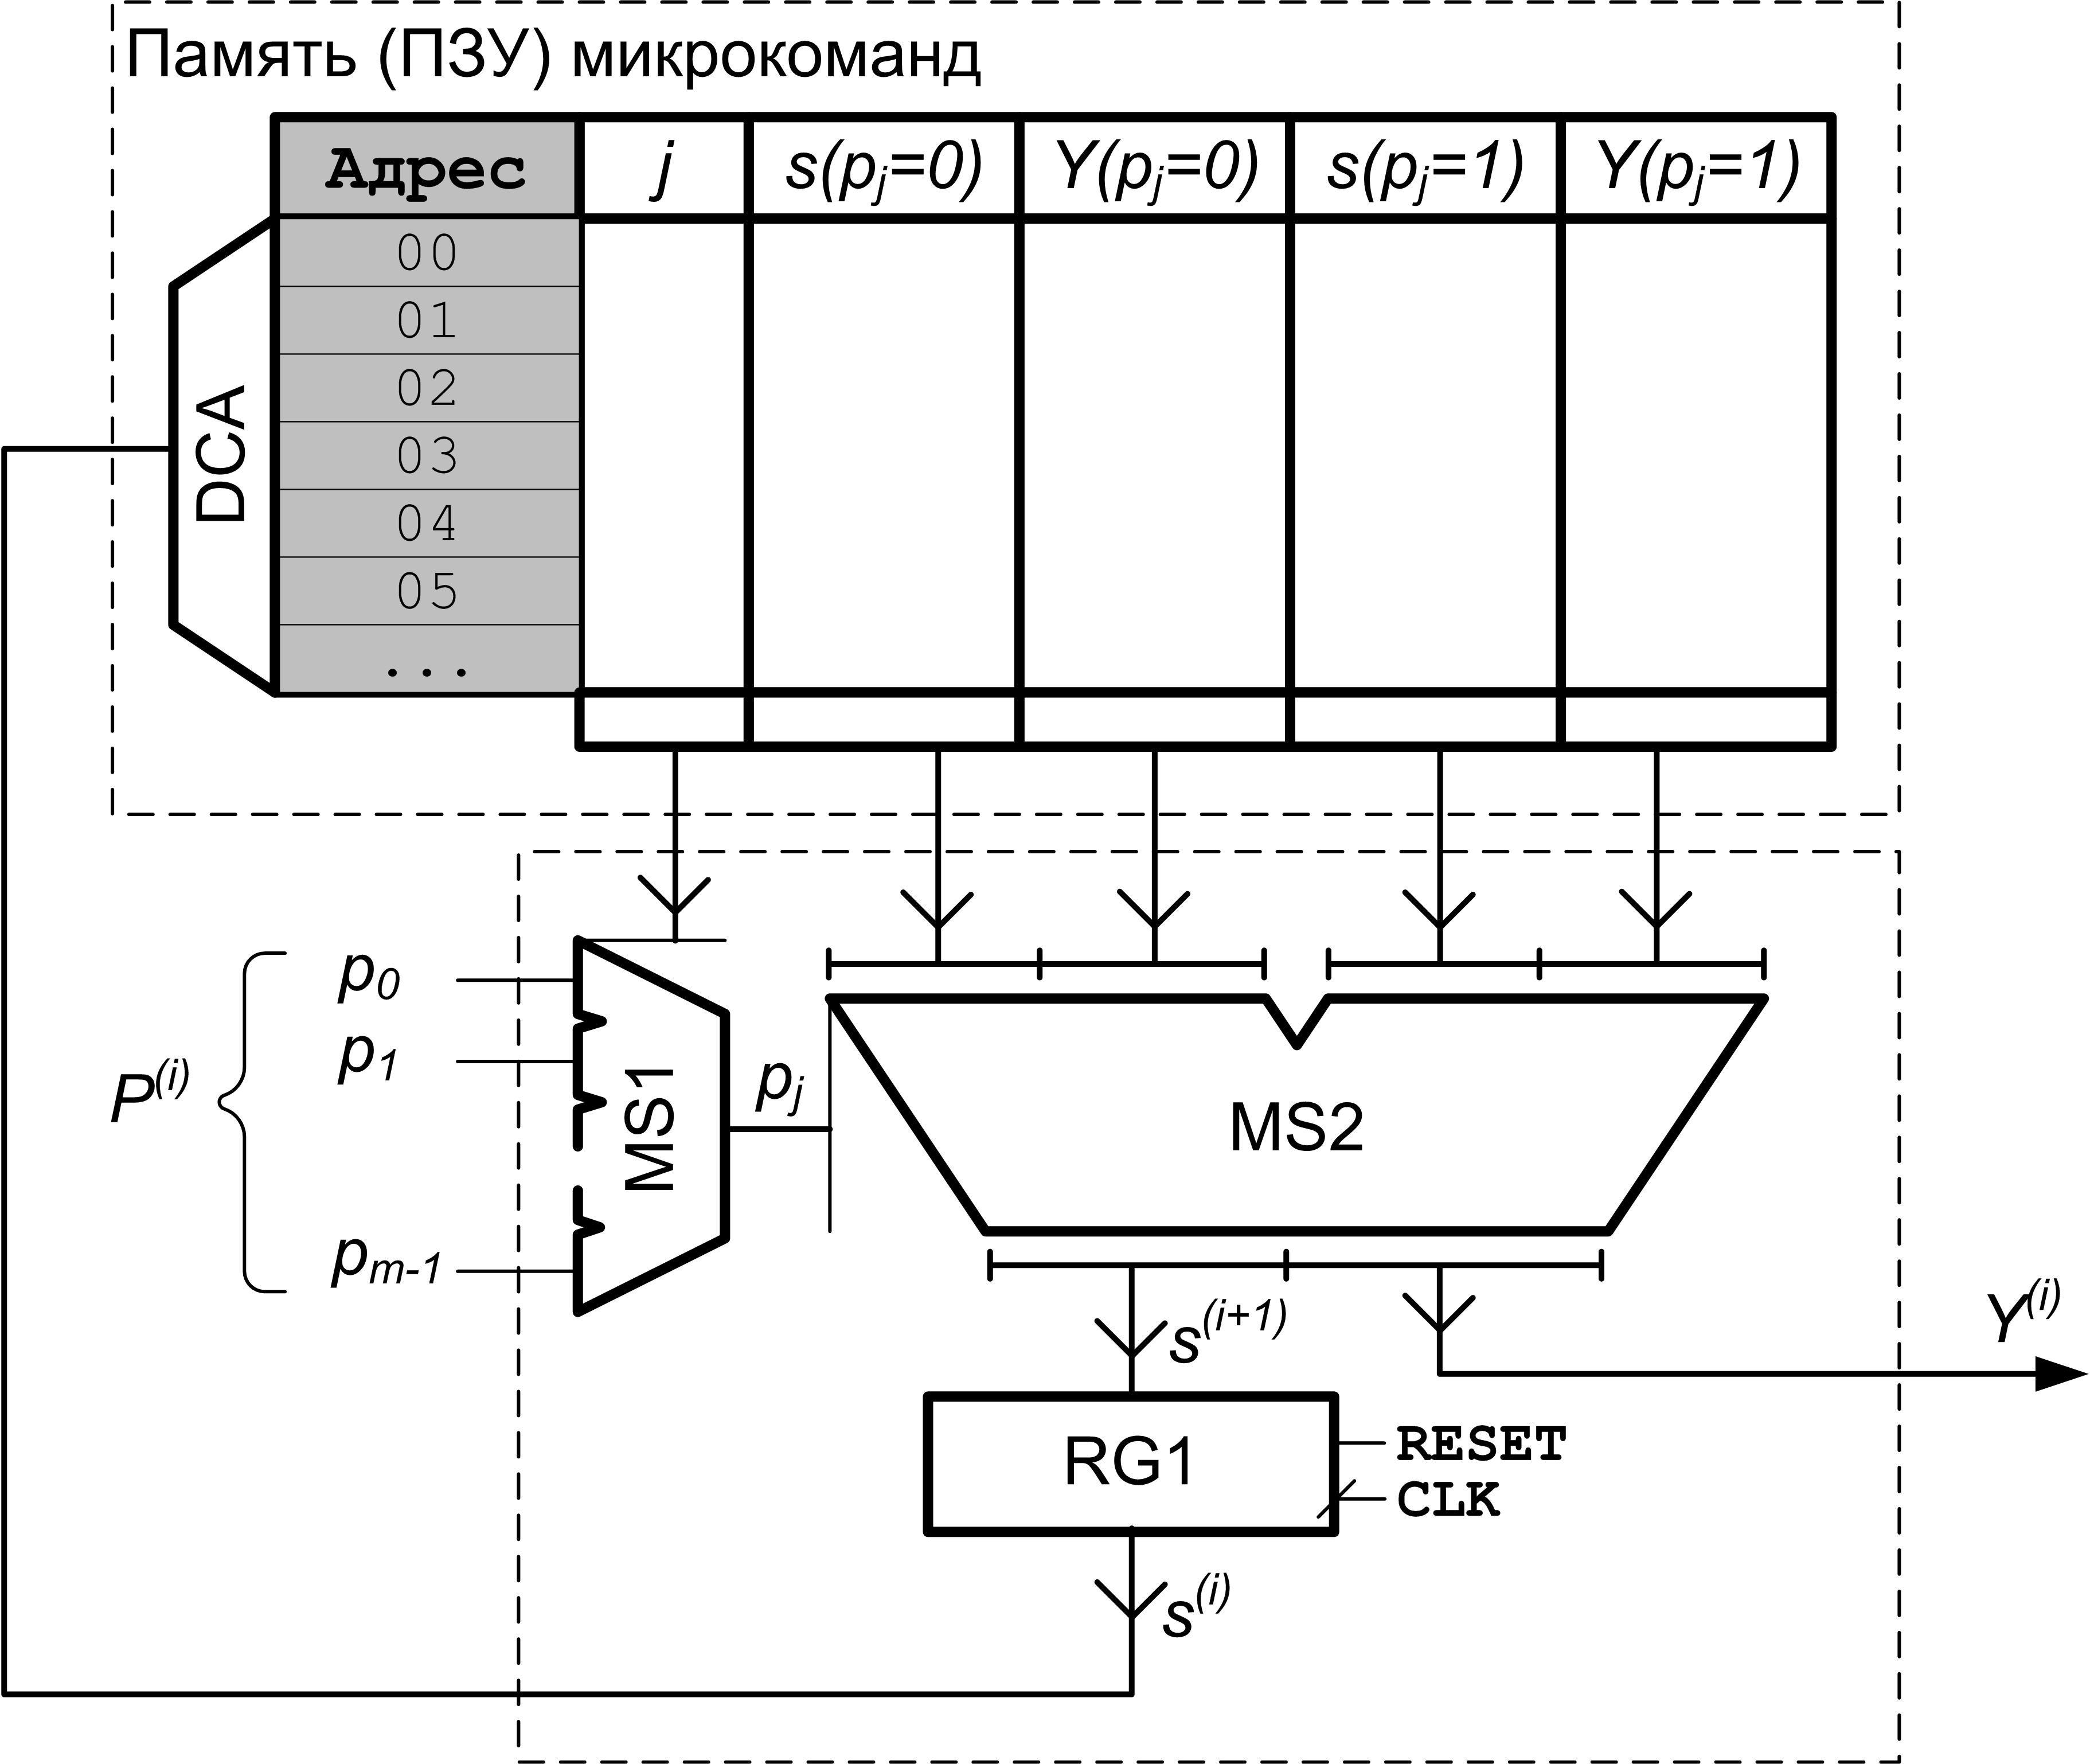
\includegraphics{fig/mili} 
    \caption{Автомат Мили}
    \label{fig::ch::practice::Mili}
\end{figure}

\begin{figure}[!ht]
    \centering
    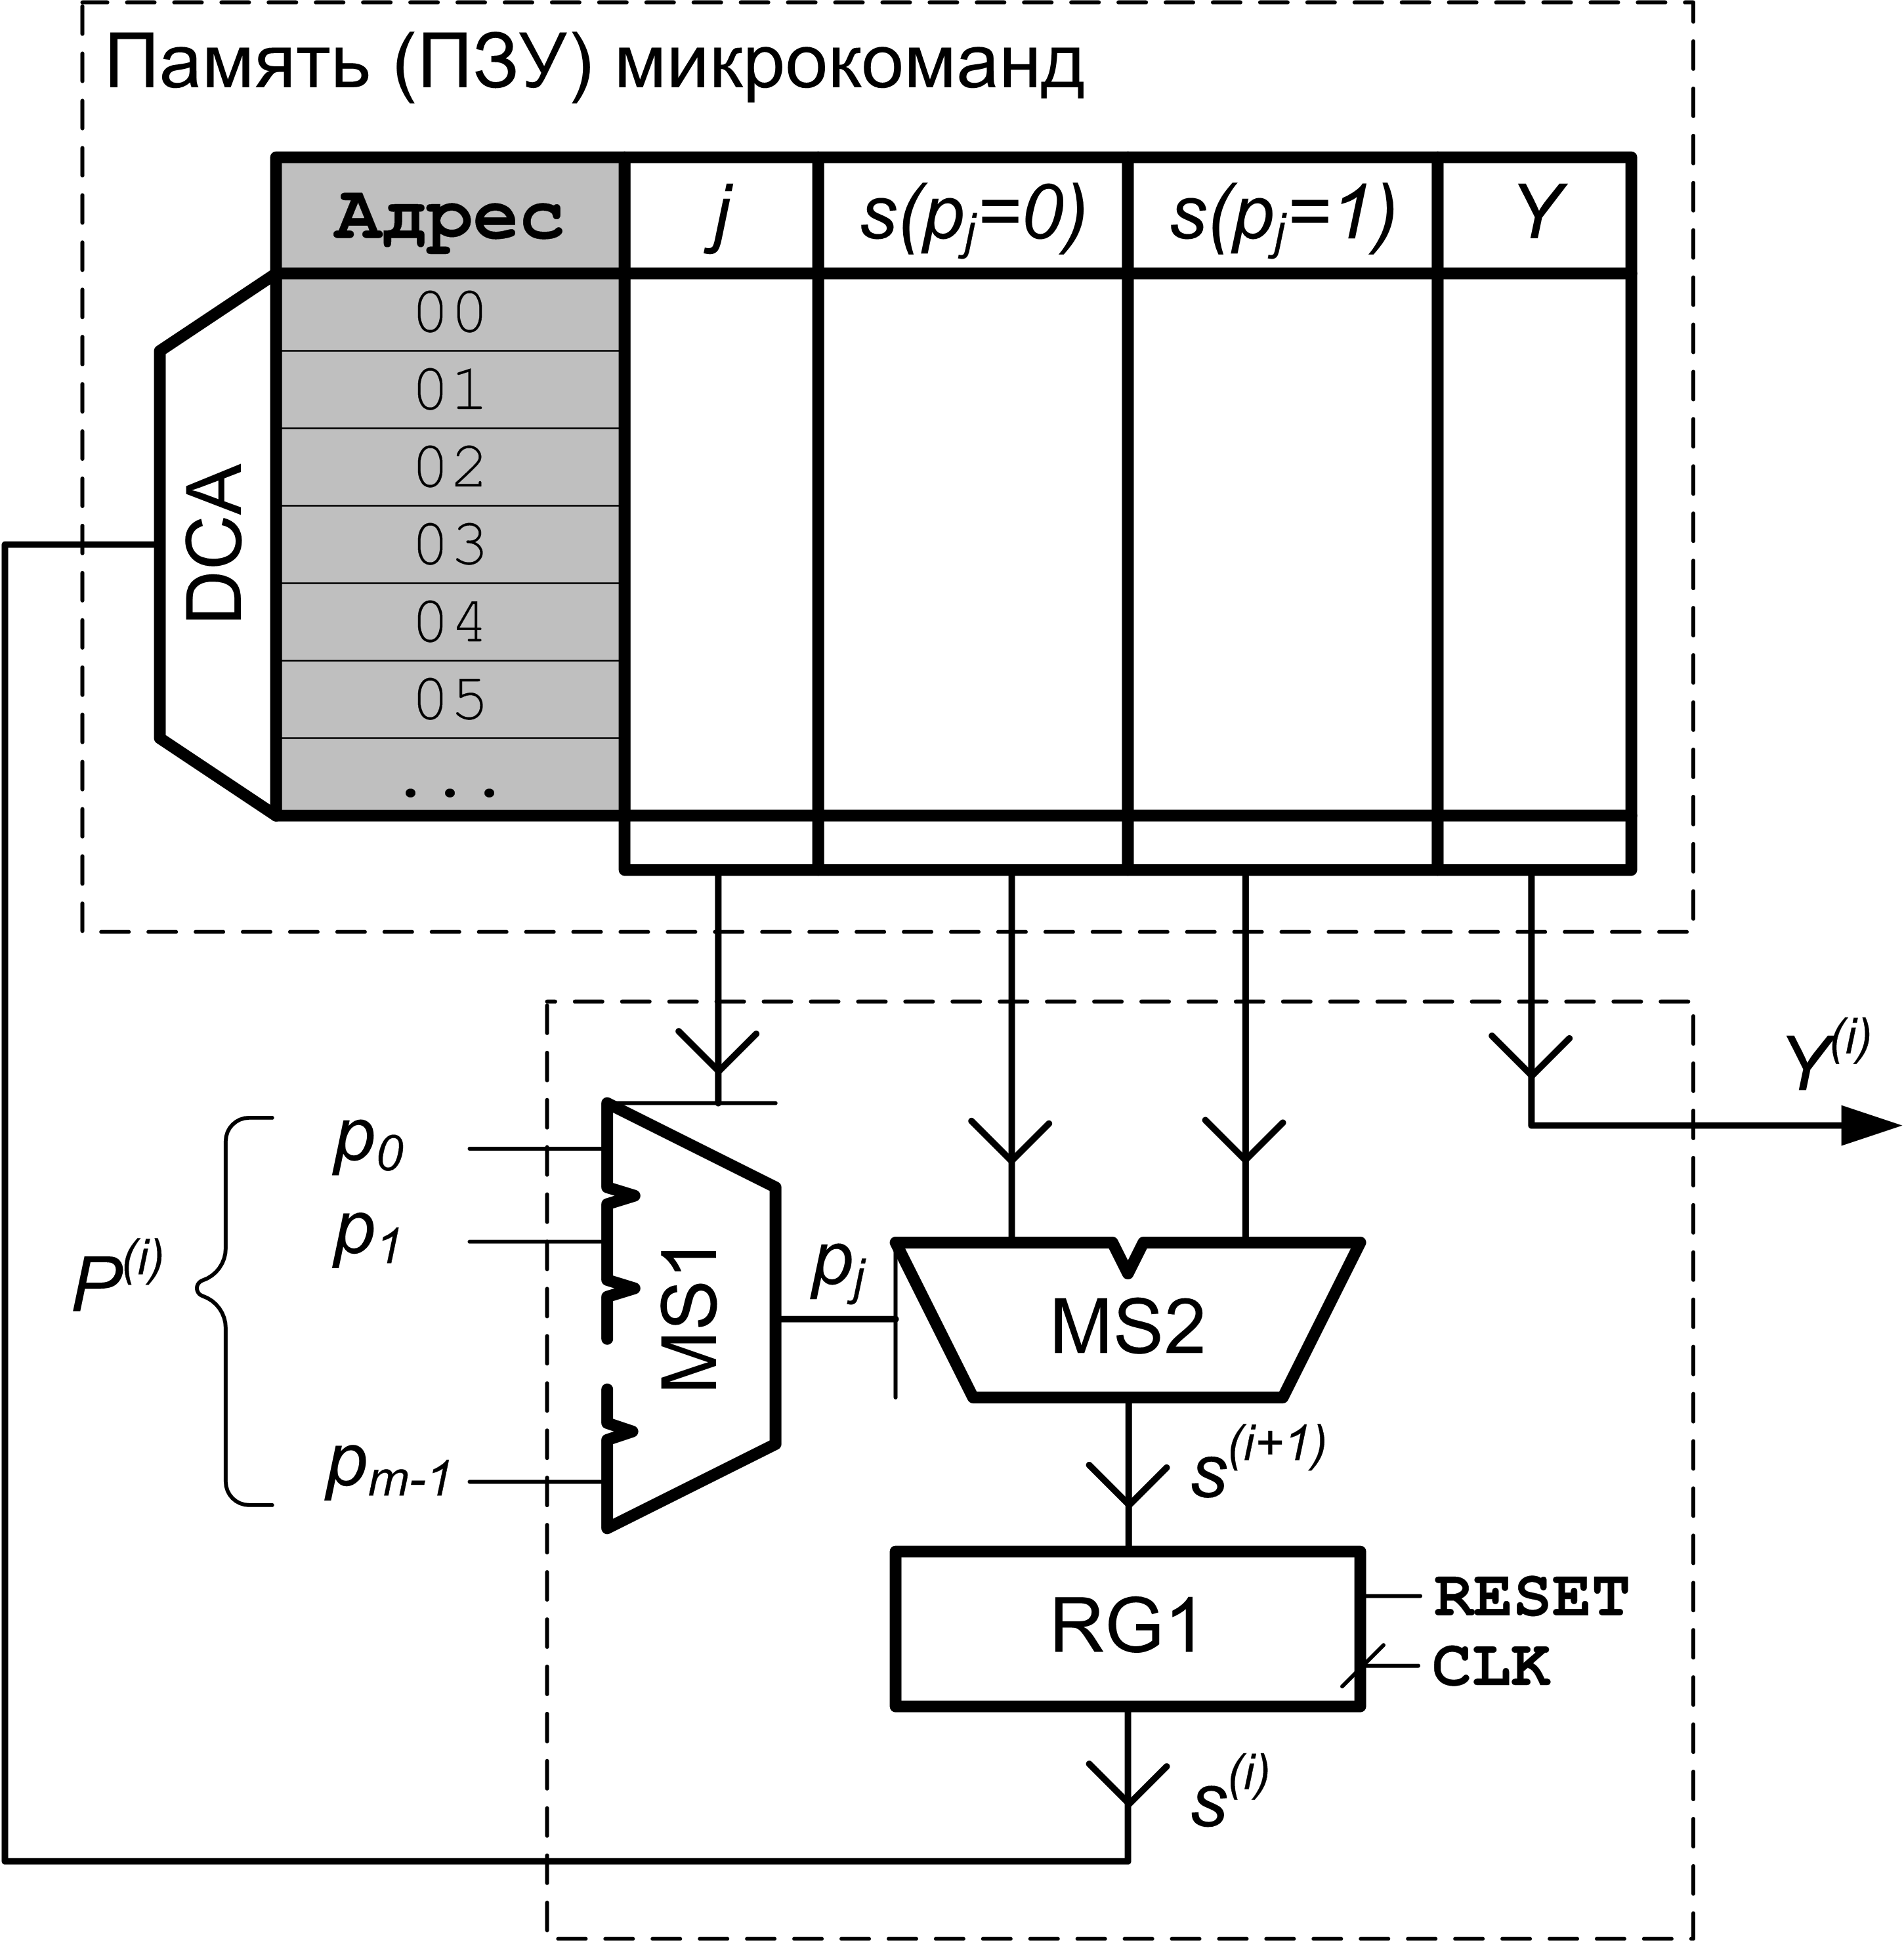
\includegraphics{fig/moore}
    \caption{Автомат Мура}
    \label{fig::ch::practice::Moore}
\end{figure}

В приведенных схемах микропрограммных автоматов выделены два блока --- <<Память (ПЗУ) микропрограмм>> и элементарное управляющее устройство. Текущему состоянию автомата $S^{(i)}$ соответствует адрес в памяти микропрограмм, то есть текущее состояние определяет адрес микрокоманды. Адрес (состояние) в течение такта снимается с выхода \Machine{RG1}. По завершению такта, в регистре \Machine{RG1} будет запомнено новое состояние, которое будет выдаваться в течение следующего такта. \Machine{RG1} переключается в каждом такте под управлением тактового сигнала \Machine{CLC}.

Ячейка памяти имеет для обоих автоматов общие части: 
\begin{itemize}
    \item поле $j$ --- выбор осведомительного сигнала (т.е. на управление \Machine{MS2} будет поступать значение осведомителного сигнала $p_j$);
    
    \item поле $S(p_j=0)$ --- новое состояние автомата, которое будет занесено в \Machine{RG1}, если $p_j=0$;
    
    \item поле $S(p_j=1)$ --- состояние, в которое перейдет автомат при $p_j=1$;    
\end{itemize}

Работа автомата начинается со сброса регистра \Machine{RG1} сигналом \texttt{RESET} в 0 --- автомат переходит в состояние $s_0$. 

Выход регистра \Machine{RG1} поступает на адресный вход памяти микрокоманд и через некоторое время значение ячейки памяти с указанным адресом поступает на выход модуля памяти. Значение поля $j$ управляет мультиплексором \Machine{MS1}, на выходе которого появляется значение осведомительного сигнала $p_j$, которое в свою очередь поступает на вход управления \Machine{MS2}. На выходе \Machine{MS2} появляется одно из двух состояний автомата: либо значение поля $S(p_j=0)$, либо --- поля $S(p_j=1)$. При переходе в следующий такт под управлением сигнала \Machine{CLC} регистр \Machine{RG1} запомнит новое состояние, сформировавшееся на выходе \Machine{MS2}.

В автомате Мили вектор управляющих сигналов снимается с выхода \Machine{MS2}, который осуществляет выбор из двух значений\footnote{
    На практике автомат Мили <<не прощает>> ошибок проектирования: когда значение сигнала $p_j$ меняется под воздействием управляющего сигнала в том же такте (такое бывает, когда значение $p_j$ снимается с выхода элемента логики, а не памяти, и соответсвенно может измениться в течение такта). Такое взаимовлияние может привести к <<гонкам>> осведомительных и управляющих сигналов и полной неопределенности в вопросе: <<в какое же из двух возможных состояний перейдет автомат Мили?>>
}, хранимых в памяти: $Y(p_j=0)$ и $Y(p_j=1)$;

В автомате Мура вектор управляющих сигналов определяется только текущим состоянием, поэтому снимается непосредственно с модуля памяти (поле $Y$).

В $i$-м такте работы управляющего устройства происходит следующее:
\begin{enumerate}
    \item Поступают осведомительные сигналы $P^{(i)}$. Эти осведомительные сигналы отражают изменения, произошедшие в предыдущем такте и в течение $i$-го такта не изменяются (так как снимаются обычно с выходов элементов памяти).
    
    \item Управляющее устройство формирует и выдает управляющие сигналы $i$-го такта. Также управляющее устройство определяет состояние $s^{(i+1)}$ в которое оно перейдет по завершении $i$-го такта. Значения управляющих сигналов стабилизируются, они распространяются по схеме и на сответствующих входях элементов памяти устанавливаются корректные значения.
    
    \item В конце такта (в зависимости от управляющих сигналов) в операционной части происходит защелкивание необходимых значений в элементах памяти. В частности, желательно сохранять в элементах памяти значения осведомительных сигналов.
\end{enumerate}

Одному такту работы схемы автомата Мили на рисунке \ref{fig::ch::practice::Mili} можно сопоставить фрагменты граф-схемы алгоритма, приведенные на рисунке \ref{fig::ch::practice::MiliAlg}. Состояния автомата выделены серыми кружками-пометками. Автомат Мили в том же такте реагирует (управляющими сигналами) на осведомительные сигналы.

\begin{figure}[!ht]
    \centering
    \begin{tabular}{c|c}
        \raisebox{-.5\height}{
            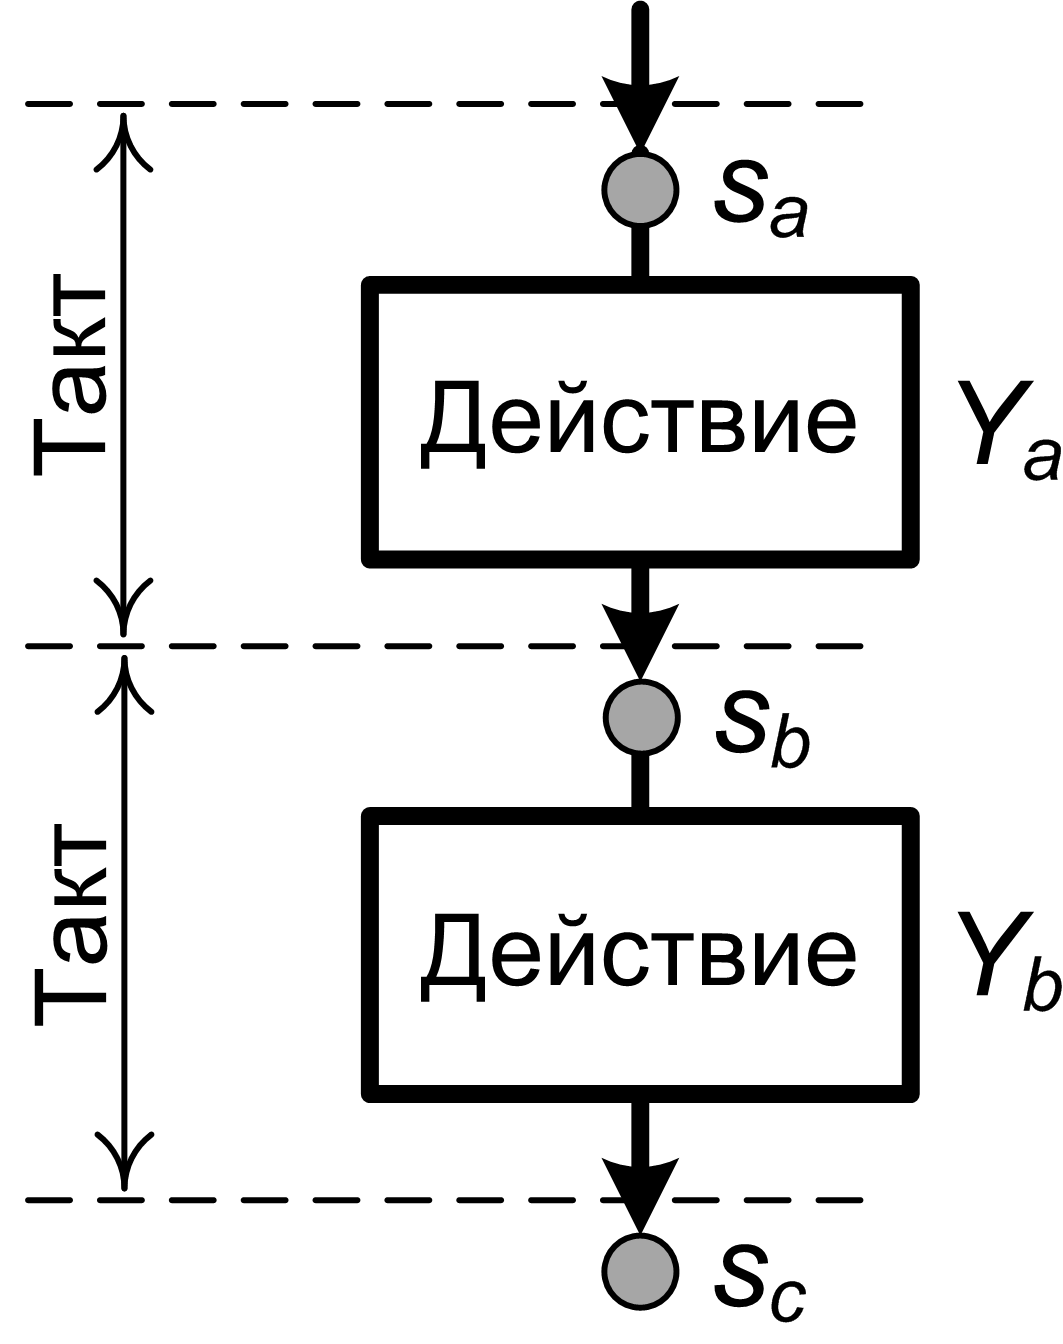
\includegraphics{fig/MiliAlgSeq}
        }
        &
			\raisebox{-.5\height}{
				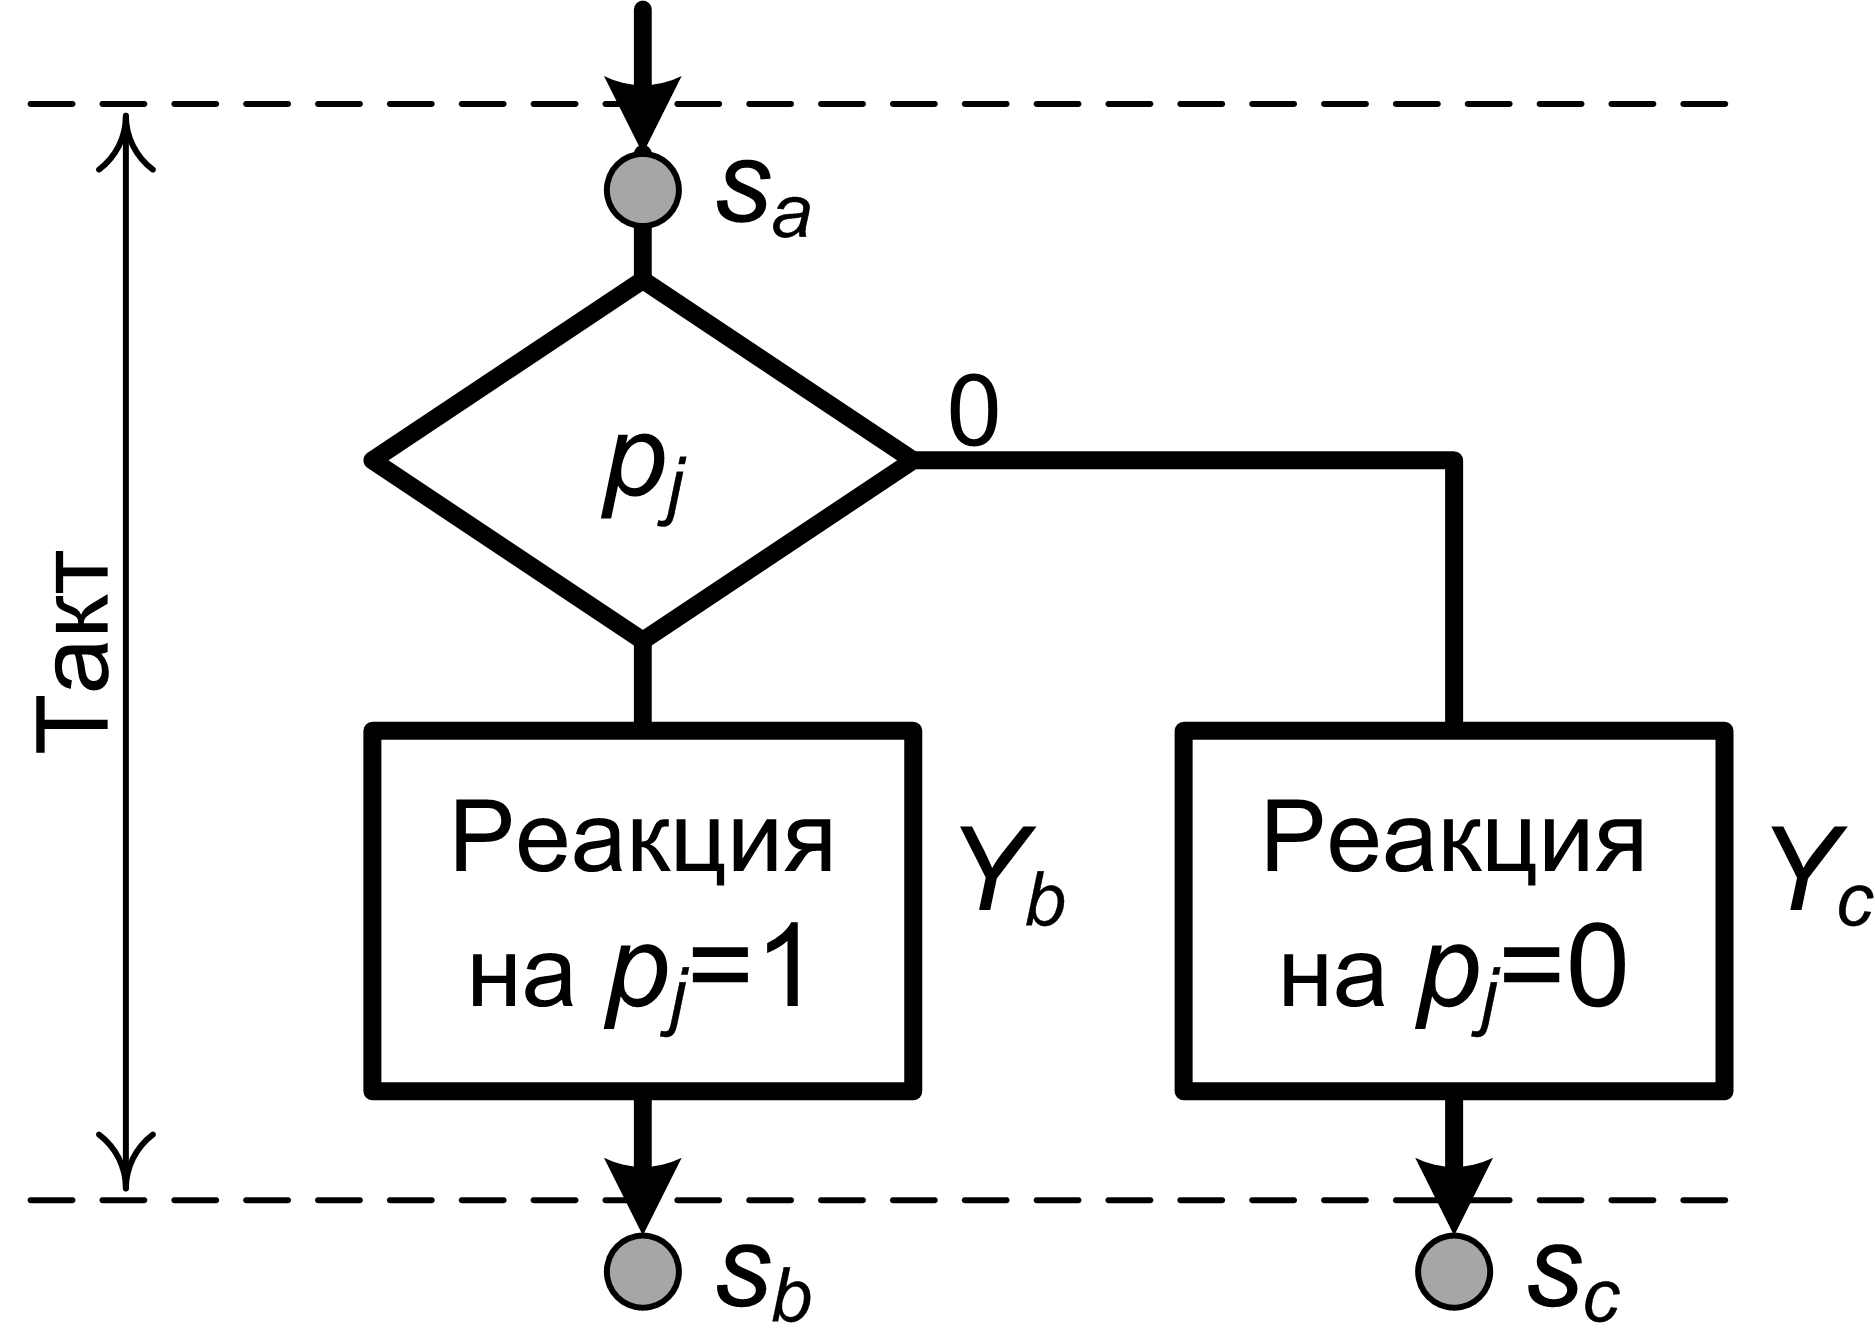
\includegraphics{fig/MiliAlgIf}
			} 
			\\
        {\xymatrix{
            S_a \ar@{->}[r]^{*|Y_a} 
                &S_b \ar@{->}[r]^{*|Y_b} 
					&S_c 
        }}
		&
			{\xymatrix{
				S_a \ar@{->}@/^/[r]^{\bar{p}_j|Y_c} 
					\ar@{->}@/_/[dr]_{p_j|Y_b} 
					&S_c \\
				*{} &S_b
			}}
			\\
    \end{tabular}
    \caption{Примеры фрагментов алгоритмов, реализуемых автоматом Мили за один такт}
    \label{fig::ch::practice::MiliAlg}
\end{figure}

Граф-схема, соответствующая такту работы автомата Мура (рис. \ref{fig::ch::practice::Moore}) приведена на рисунке \ref{fig::ch::practice::MooreAlg}. Автомат Мура реагирует на осведомительные сигналы только в следующем такте. 

\begin{figure}[!ht]
    \centering
    \begin{tabular}{c|c}
        \raisebox{-.5\height}{
            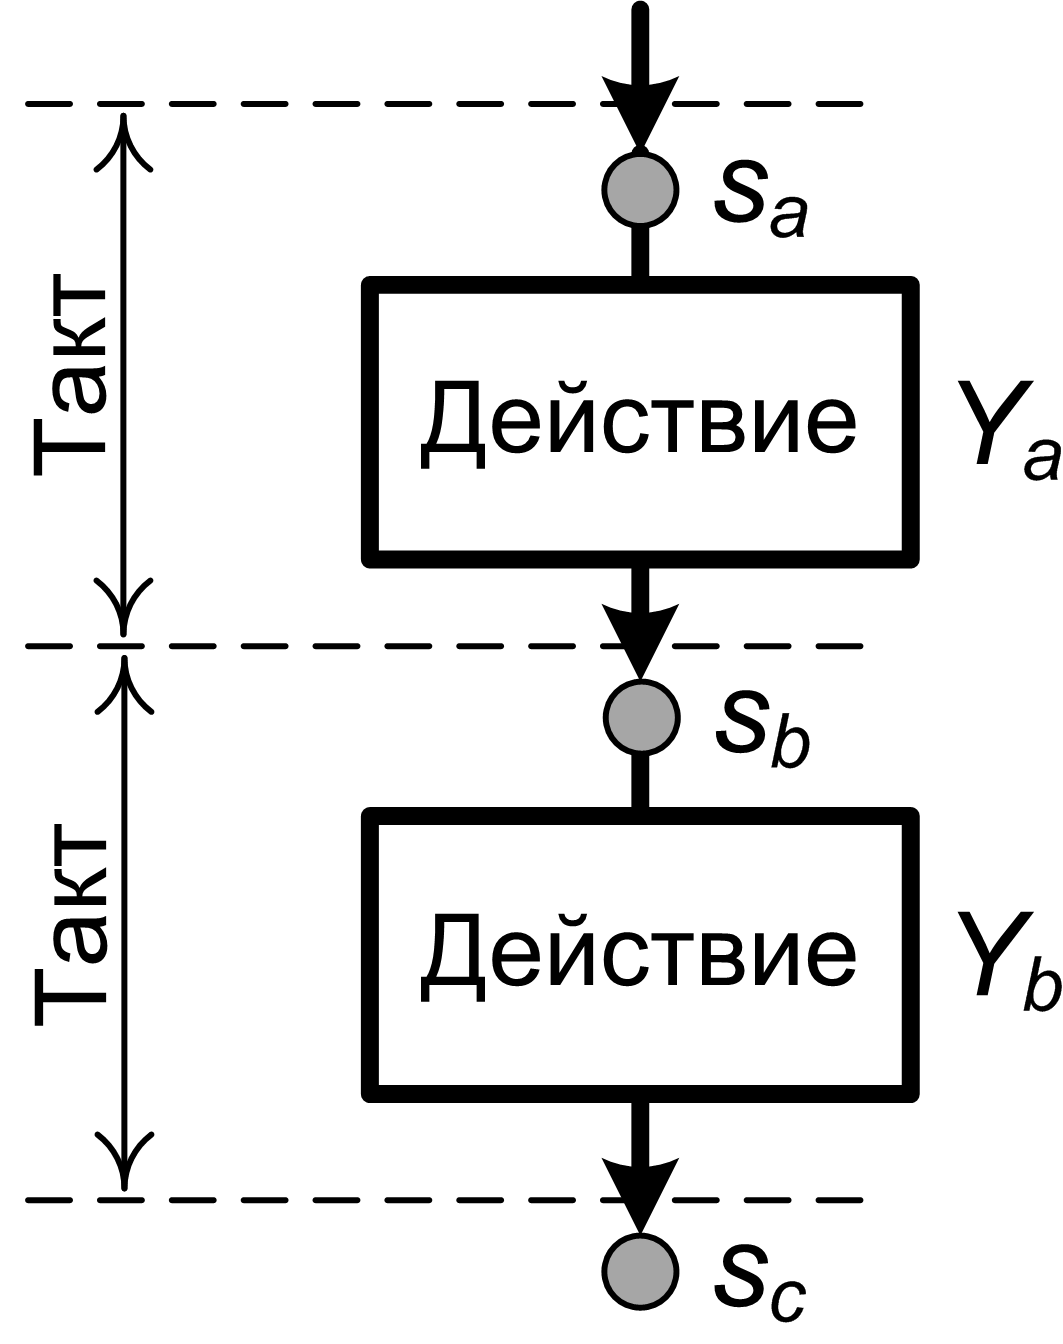
\includegraphics{fig/MooreAlgSeq}
        }
        &
			\raisebox{-.5\height}{
                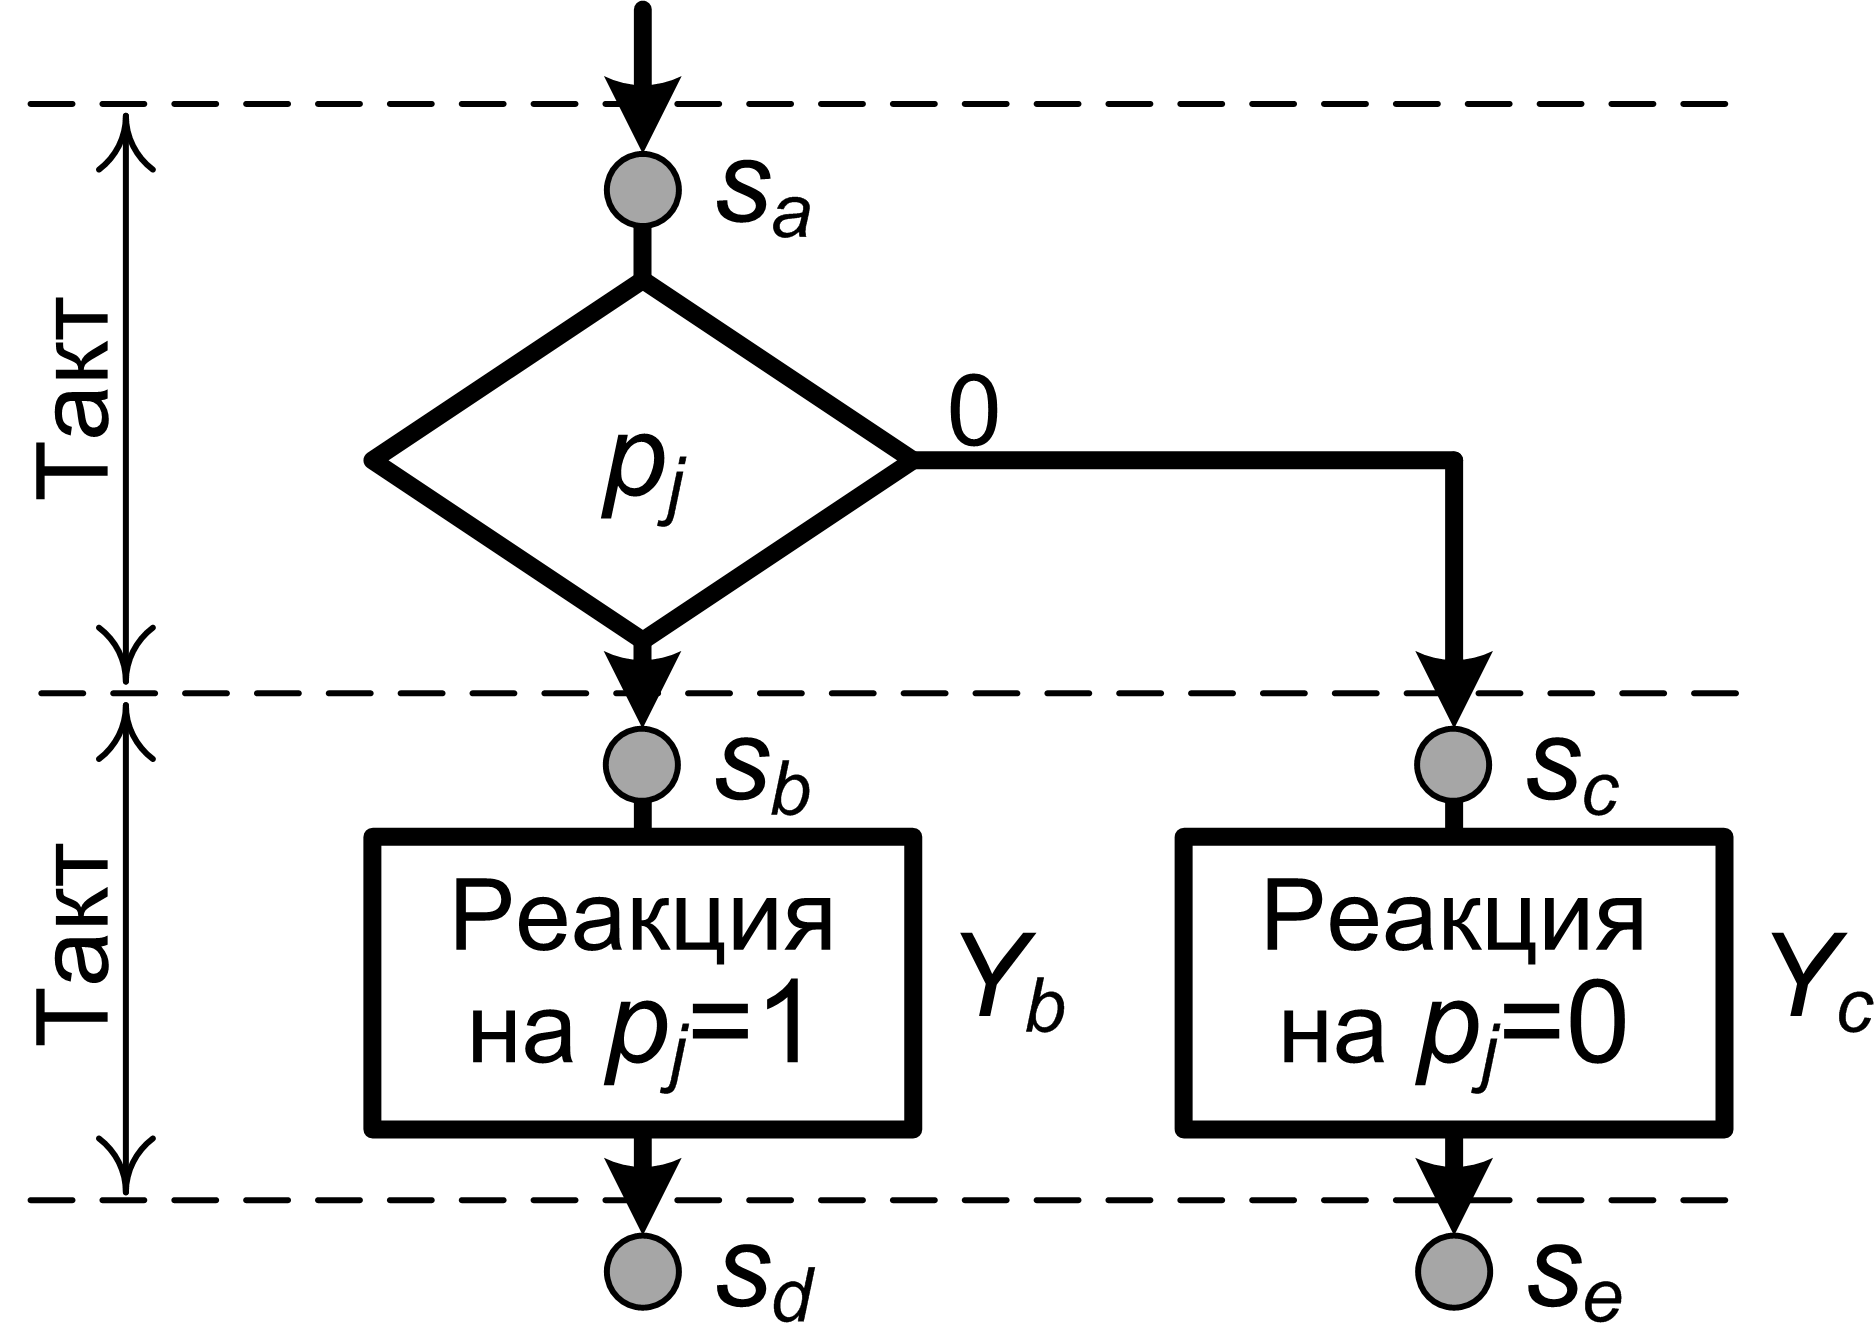
\includegraphics{fig/MooreAlgIf}
            }
			\\
        {\xymatrix{
            S_a|Y_a \ar@{->}[r]^{*} 
                &S_b|Y_b \ar@{->}[r]^{*} 
                    &S_c| \\
        }}
        &
            {\xymatrix{
                S_a|\Machine{0h} \ar@{->}@/^/[r]^{\bar{p}_j} 
                    \ar@{->}@/_/[dr]_{p_j} 
                    &S_c|Y_c \ar@{->}[r]^{*} 
                        &S_e|
                        \\
                *{} 
                    &S_b|Y_b \ar@{->}[r]^{*} 
                        &S_d|
            }}            
    \end{tabular}
    \caption{Примеры фрагментов алгоритма, реализуемых автоматом Мура за один такт}
    \label{fig::ch::practice::MooreAlg}
\end{figure}

Видно, что автомат Мура тратит отдельный такт на анализ осведомительного сигнала, при этом в таком такте, конечно могут выдаваться и управляющие сигналы (в приведенном примере на Рис. \ref{fig::ch::practice::MooreAlg} выдается \Machine{0h}). То есть, можно совместить вершину процесса и условную вершину в одном состоянии, если процесс на условие не влияет и тогда процесс и анализ условия \emph{совмещаются} во времени. В противном случае, если имелось в виду, что \emph{после} определенных действий, следует проанализировать осведомительный сигнал, то следует выделить два состояния (см. пример на рисунке \ref{fig::ch::practice::MooreAlgFictive}).
\begin{figure}[!ht]
    \centering
    \begin{tabular}{c|c}
        \raisebox{-.5\height}{
            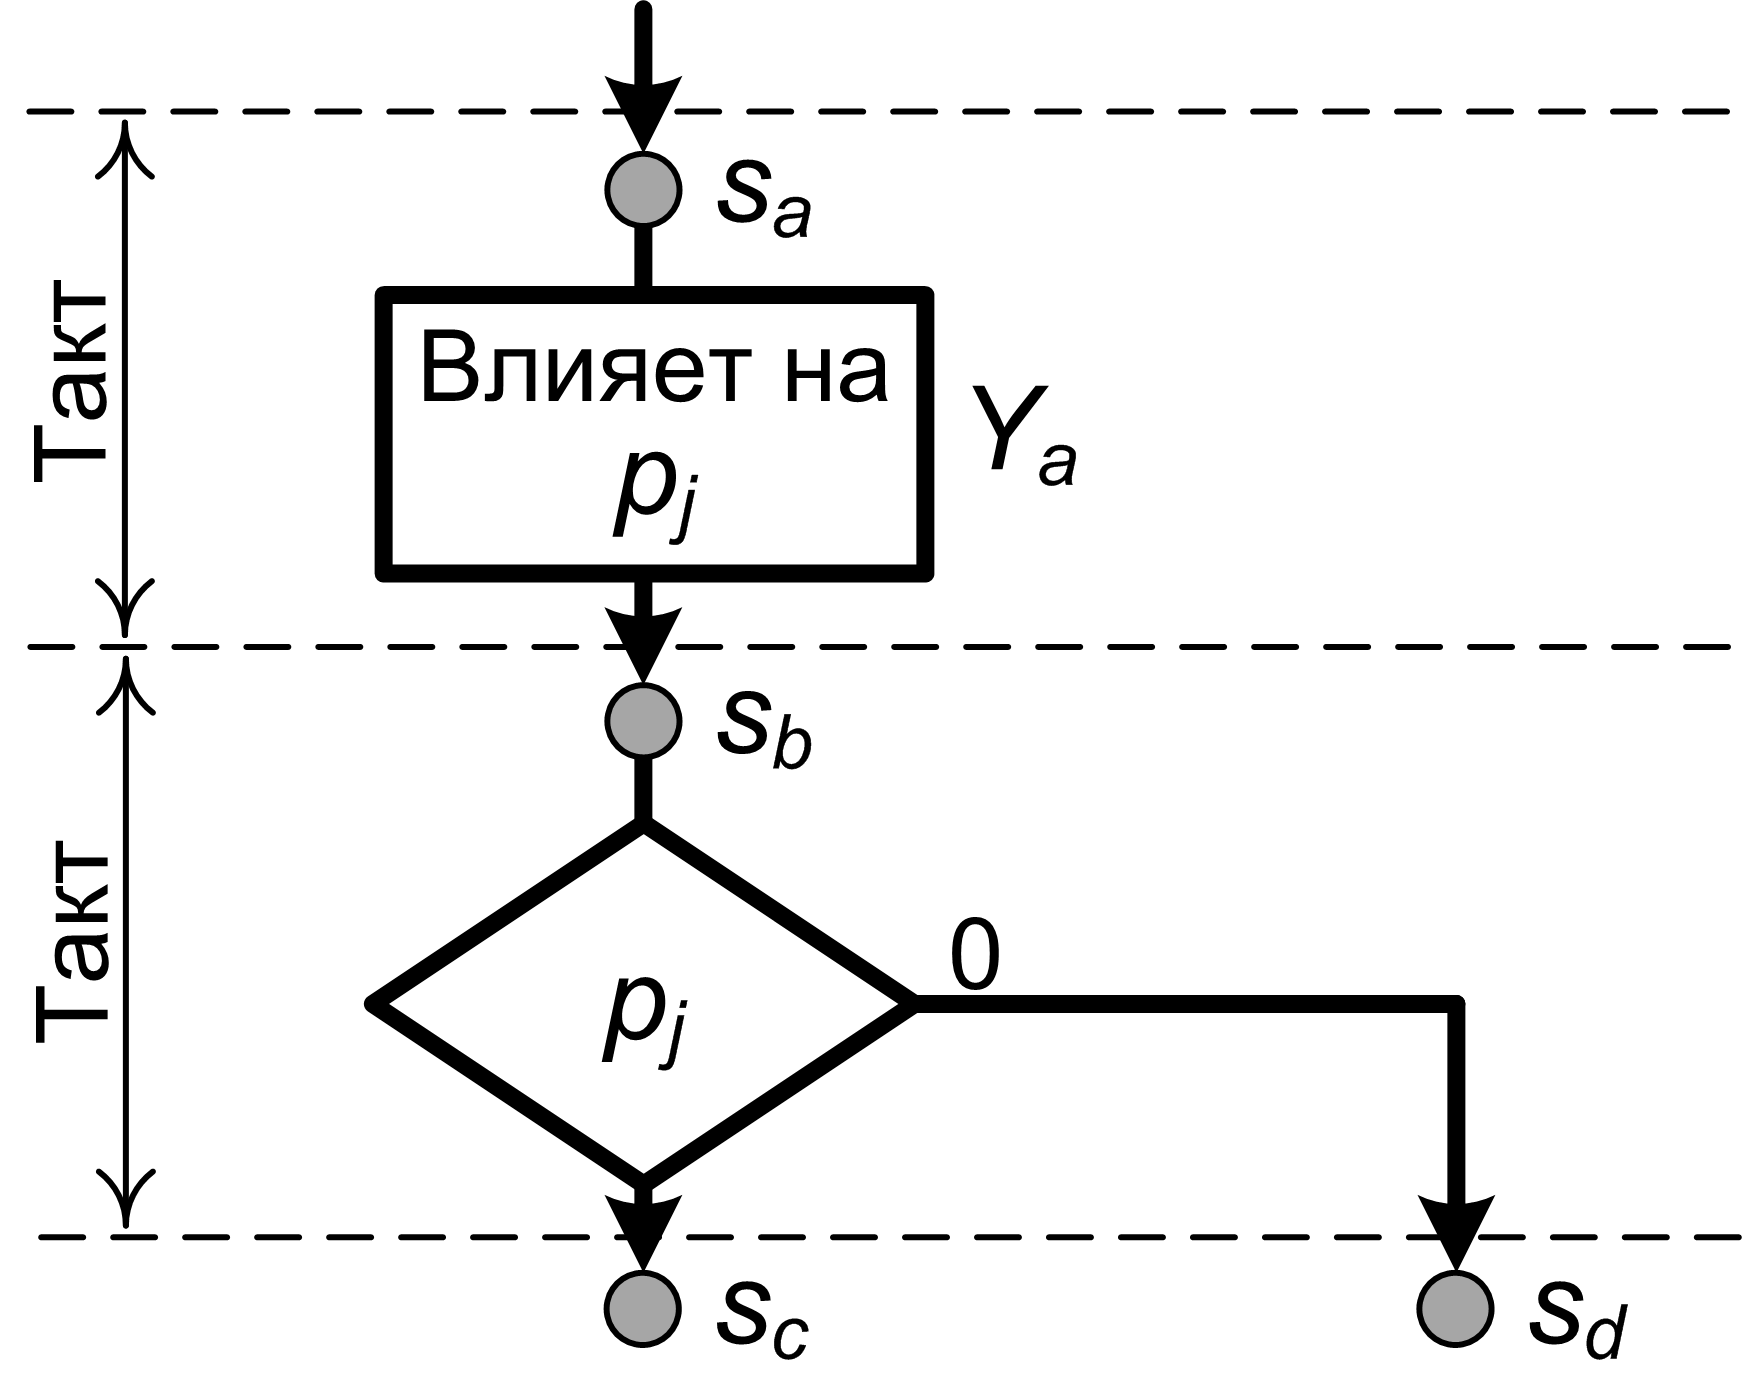
\includegraphics{fig/MooreIfTwo}
        }
        &
			\raisebox{-.5\height}{
                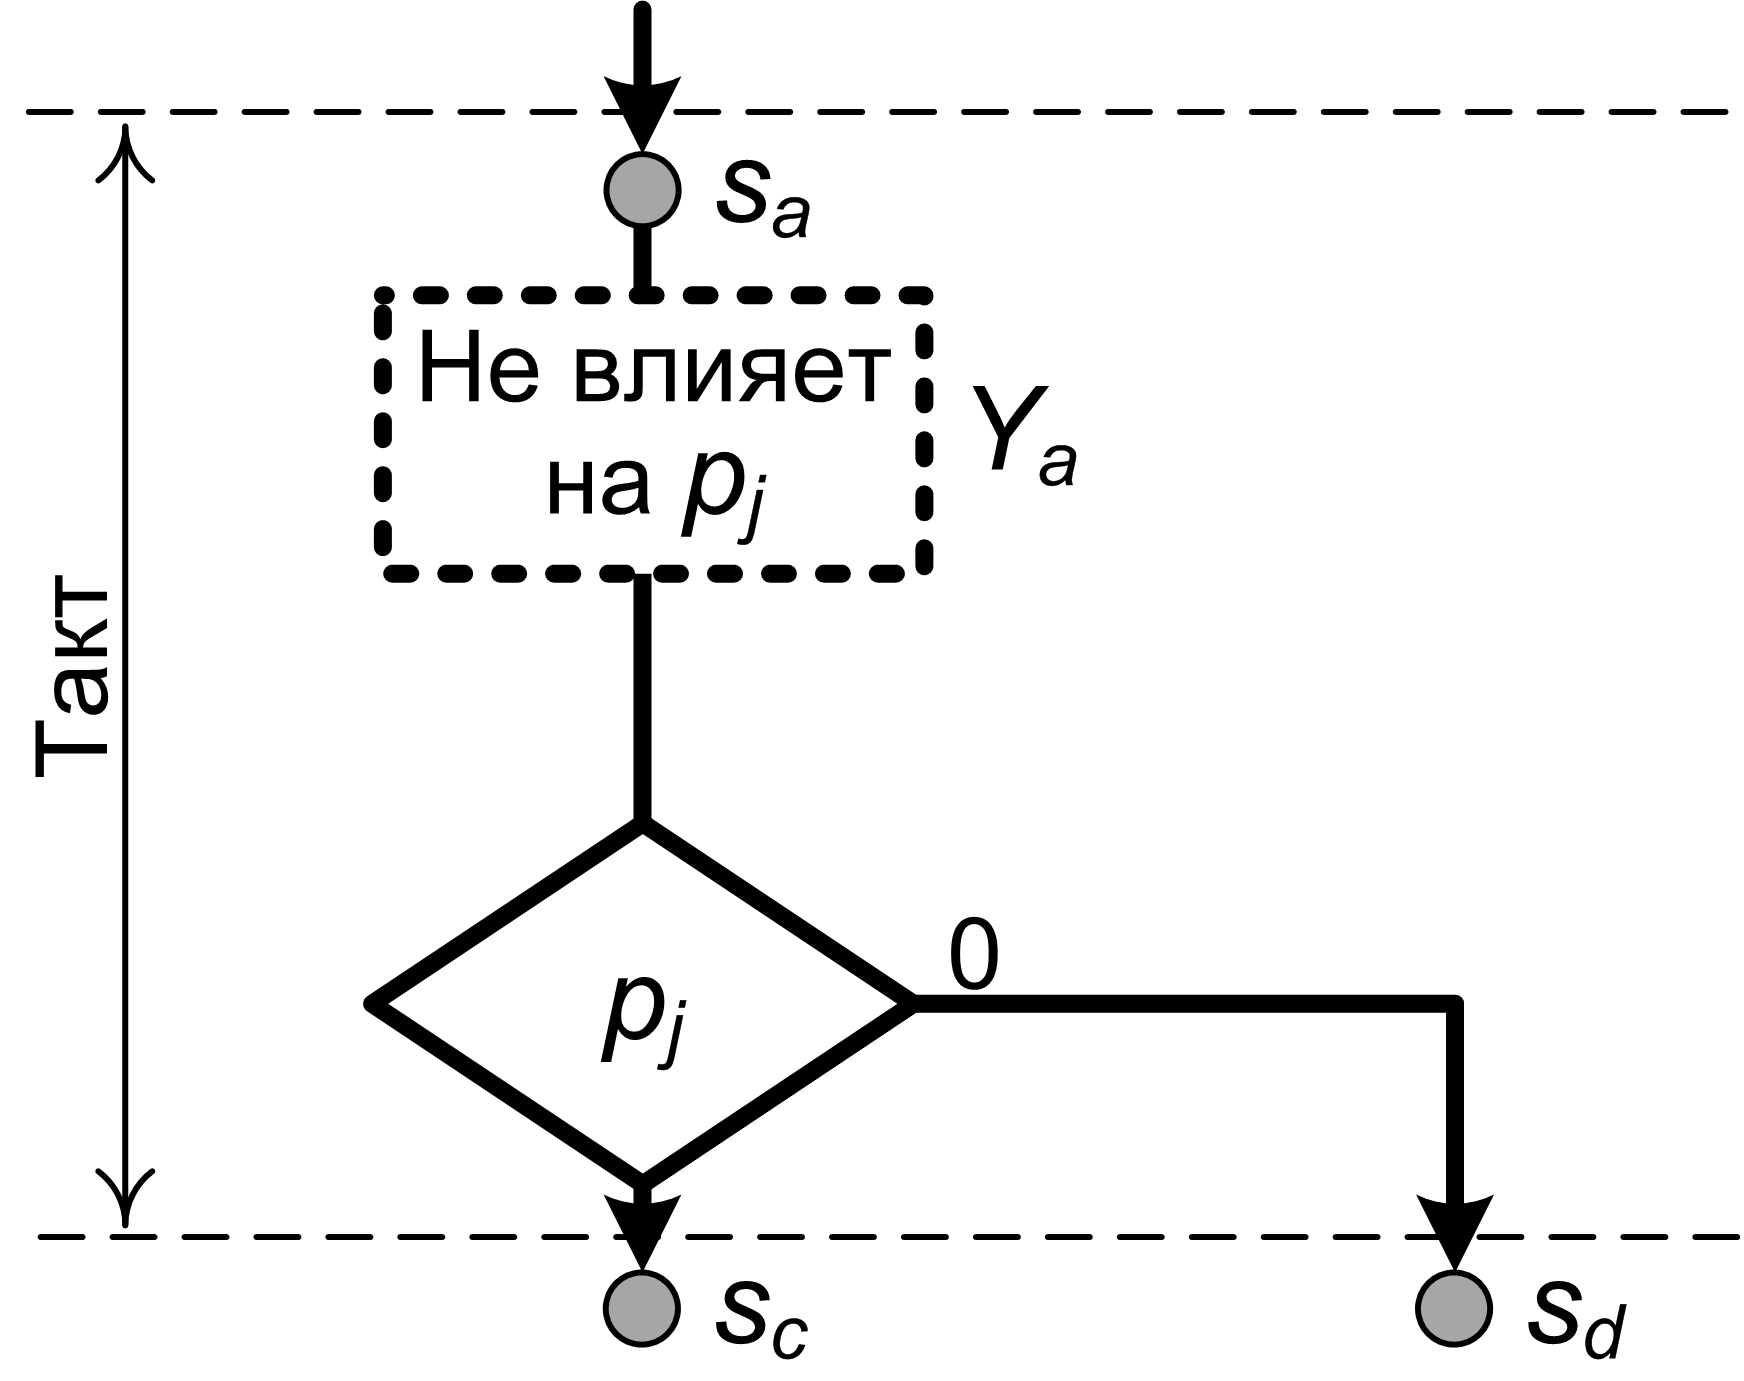
\includegraphics{fig/MooreIfOne}
            }
			\\
        {\xymatrix{
            S_a|Y_a \ar@{->}[r]_{*} 
                &S_b|\Machine{0h} \ar@{->}@/^/[r]^{\bar{p}_j}  
                                  \ar@{->}@/_/[dr]_{p_j} 
                    &S_d|
                    \\
            *{} 
                &*{}
                    &S_c|
        }}            
        &
            {\xymatrix{
                S_a|Y_a \ar@{->}@/^/[r]^{\bar{p}_j}  
                                      \ar@{->}@/_/[dr]_{p_j} 
                    &S_d|
                    \\
                *{}
                    &S_c|
        }}            
    \end{tabular}
    \caption{Особенности выделения состояний автомата Мура}
    \label{fig::ch::practice::MooreAlgFictive}
\end{figure}


На указанные фрагменты можно разбить любую произвольную схему алгоритма. Также при составлении алгоритма следует учитывать указанные особенности автомата, выполняющего этот алгоритм. Детальное обсуждение особенностей находится за рамками данного курса, поэтому далее рассматривается пример микропрограммирования, который позволить понять суть микропрограммного управления.

\subsection{Соглашения о взаимодействии с ЦУУ}

Особенности взамодействия ОЧ множительного устройства и ЦУУ были изложены в самом начале раздела \ref{ch::practice}. Введем следующие обозначения сигналов:
\begin{itemize}
    \item $p_0\Machine{(TASK)}$ --- <<Задание на шине>> от ЦУУ;
    \item $p_1\Machine{(BUS)}$ --- <<Шина твоя>> от ЦУУ;
    \item $y_0\Machine{(READY)}$ --- <<Свободен>> в ЦУУ;
    \item $y_1\Machine{(RESULT)}$ --- <<Результат готов>> в ЦУУ;
    \item \Machine{CLK} --- тактовые импульсы, синхронизирующие все устройства вычислительной системы в целом;
    \item \Machine{X(DATA)} --- данные на шине данных, могут выдаваться как ЦУУ (исходные операнды), так и множительным устройством (результат).
\end{itemize}

Изменение сигналов принято изображать на временной диаграмме. Высокий уровень сигнала на диаграмме соответствует логической единице, низкий --- нулю.

\begin{figure}[!ht]
    \centering
    \includegraphics{fig/timings.1}
    \caption{Временная диаграмма получения задания}
    \label{fig::ch::practice::timingsTr}
\end{figure}

Состояние шины (жгута) изображается по особому: так как на диаграмме обычно нет места, чтобы изобразить все линии шины по отдельности, то состояние шины изображают как один сигнал (см. сигнал \Machine{X(DATA)}). Когда состояние шины не имеет значения (на рисунке \ref{fig::ch::practice::timingsTr} это такты 0 и 3), то рисуют линию посередине между высоким и низким уровнем. При этом по шине могут передаваться данные для других устройств.

Когда на шину поступают данные, которые важны, их изображают двумя линиями, проведенными на высоком и низком уровнях одновременно (такты 1, 2 на рисунке \ref{fig::ch::practice::timingsTr}), а если нужно указать значение двоичного вектора на шине, то между линиями пишут соответствующее шестнадцатиричное значение.

На рисунке \ref{fig::ch::practice::timingsTr} изображена временная диаграмма получения задания от ЦУУ. Устройства следуют следующим соглашениям.
\begin{enumerate}
    \item УЧ выдает в ЦУУ сигнал $y_0\Machine{(READY)}$. См. такт 1. Таким образом УЧ сообщает ЦУУ, что множительное устройство готово решать новую задачу. Сигнал будет удерживаться до тех пор, пока ЦУУ не даст задание. 
    
    \item Когда ЦУУ потребуется выполнить умножение, то оно, убедившись, что множительное устройство готово ($y_0=1$), выдает в УЧ сигнал $p_0\Machine{(TASK)}$. См. такт 3. В последующих тактах ЦУУ будет выдавать фрагменты задания $\Machine{D}_1,\ldots,\Machine{D}_n$. В общем случае, задание состоит из одного фрагмента.
    
    ЦУУ выдает сигнал $p_0\Machine{(TASK)}$ только в течение одного такта.
    
    \item УЧ \emph{должна} в следующем такте, после получения сигнала  $p_0\Machine{(TASK)}$ от ЦУУ снять сигнал $y_0\Machine{(READY)}$ и начать чтение с шины первого фрагмента задания. См. такт 4. Пока УЧ решает задачу, сигнал $y_0\Machine{(READY)}$ не должен выдаваться.
\end{enumerate}

На рисунке \ref{fig::ch::practice::timingsRr} изображена временная диаграмма выдачи результата в ЦУУ. 

\begin{figure}[!ht]
    \centering
    \includegraphics{fig/timings.2}
    \caption{Временная диаграмма выдачи результата}
    \label{fig::ch::practice::timingsRr}
\end{figure}

\begin{enumerate} 
    \item УЧ выдает в ЦУУ сигнал $y_1\Machine{(RESULT)}$. См. такт 1. УЧ будет ждать момента, когда ЦУУ освободит шину и будет удерживать этот сигнал, пока не получит разрешение на передачу. См. такты 1-3. Количество тактов, в течение которых ЦУУ освобождает шину, варьируется, и непоправимой ошибкой будет выдача результата на <<занятую>> шину.

    \item ЦУУ, убедившись, что результат готов, выдает в течение одного такта сигнал $p_1\Machine{(BUS)}$. См. такт 3.
    
    \item УЧ, приняв сигнал $p_1\Machine{(BUS)}$ в следующем такте \emph{должно} снять сигнал $y_1\Machine{(RESULT)}$ и начать выдавать первый фрагмент результата. См. такт 4.
    
    \item УЧ как можно раньше должно выдать в ЦУУ сигнал $y_0\Machine{(READY)}$. Обычно, сигнал $y_0\Machine{(READY)}$ выдается в том же такте, в котором выдается последний фрагмент результата. См. такт $(n+3)$.
\end{enumerate}


\subsection{Пример микропрограммирования}
\label{ss::ch::practice::software::example}

В качестве примера рассматривается задача получения дополнительного кода из прямого. Несомненно, эту задачу можно решить проще.

Операционная часть устройства приведена на рисунке \ref{fig::ch::practice::dcconverter}.

\begin{figure}[!ht]
    \centering
    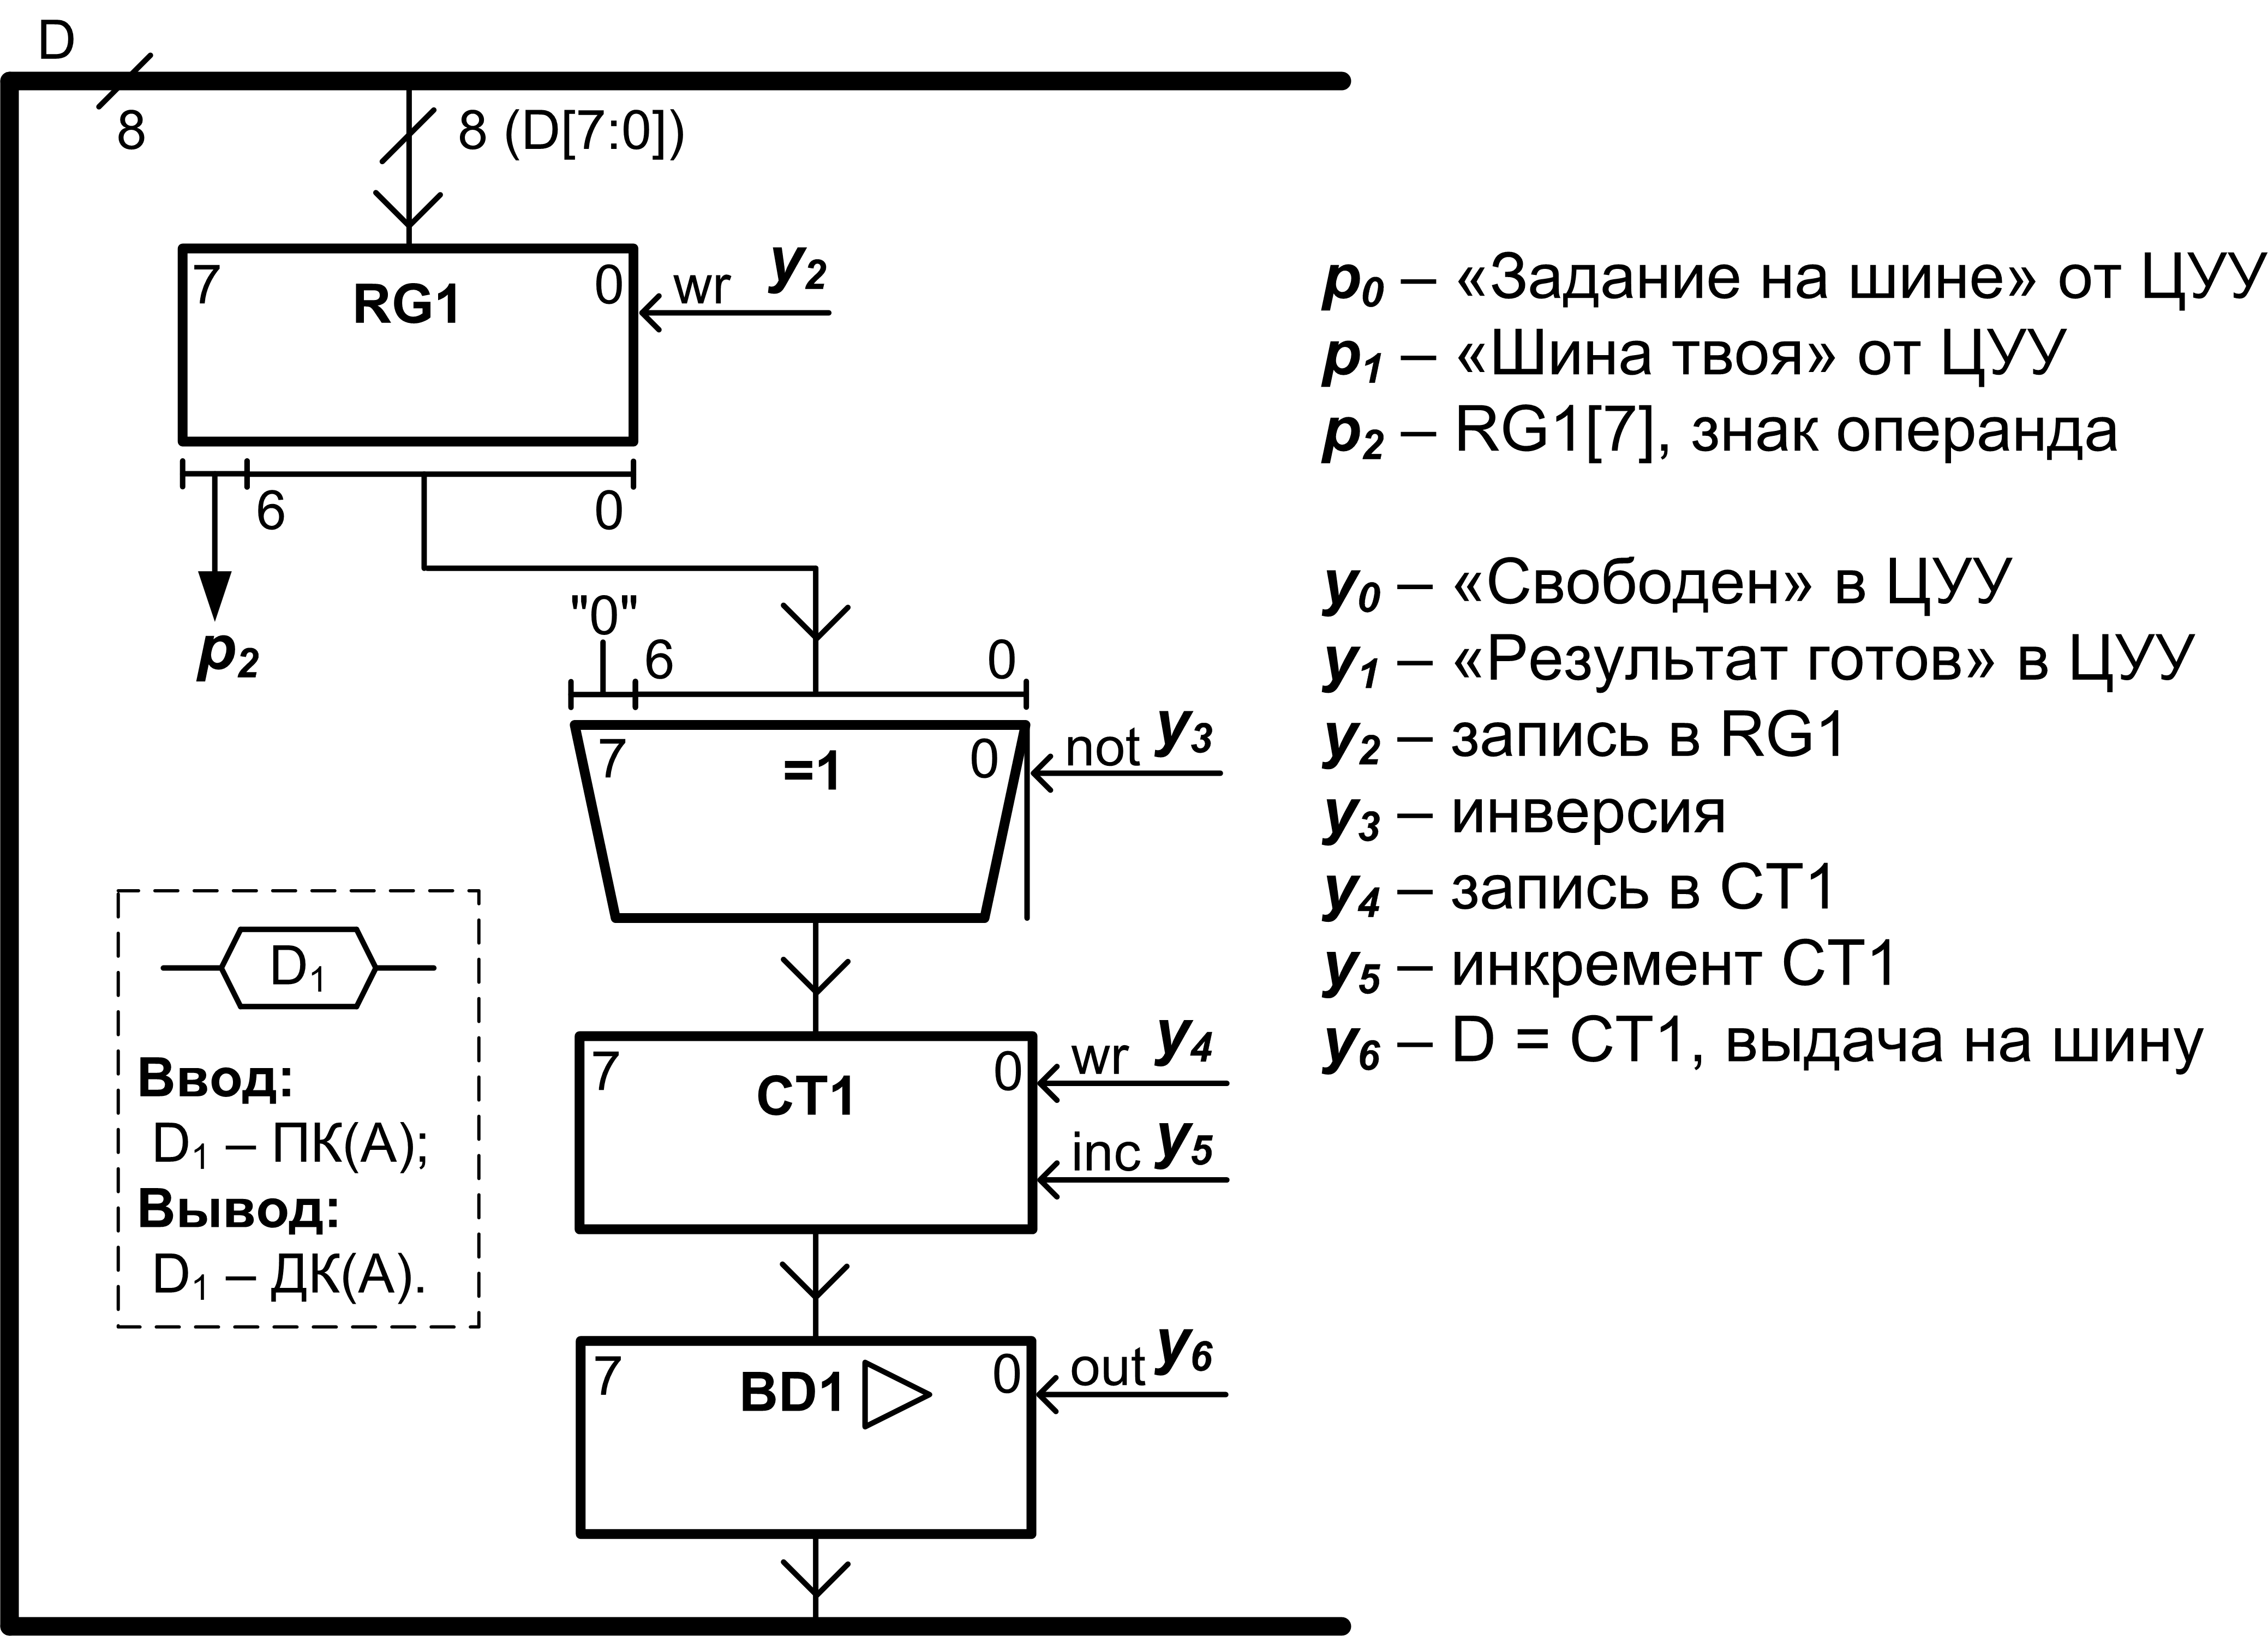
\includegraphics{fig/dcconverter}
    \caption{Операционная часть преобразователя $\Machine{ПК}\mapsto\Machine{ДК}$}
    \label{fig::ch::practice::dcconverter}
\end{figure}

Назначение осведомительных и управляющих сигналов следующее:
\begin{itemize}
    \item $p_0\Machine{(TASK)}$ --- <<Задание на шине>> от ЦУУ;
    \item $p_1\Machine{(BUS)}$ --- <<Шина твоя>> от ЦУУ;
    \item $y_0\Machine{(READY)}$ --- <<Свободен>> в ЦУУ;
    \item $y_1\Machine{(RESULT)}$  --- <<Результат готов>> в ЦУУ;
    
    \item $p_2$ --- \Machine{RG1[7]}, знак операнда;
    \item $y_2$ --- запись в \Machine{RG1}
    \item $y_3$ --- инверсия;
    \item $y_4$ --- запись в \Machine{CT1};
    \item $y_5$ --- инкремент \Machine{CT1};
    \item $y_6$ --- \Machine{X=CT1}, выдача результата на шину.
\end{itemize}

С помощью данной операционной части задачу можно решить так:
\begin{enumerate}
    \item получить задание и записать операнд в \Machine{RG1} ($y_2$); 
    \item если знак операнда $p_2=0$, то перейти к шагу \ref{en:ch::practice::dcconverter:positive}, иначе к шагу \ref{en:ch::practice::dcconverter:negative};
    \item \label{en:ch::practice::dcconverter:positive} записать модуль операнда в \Machine{CT1} ($y_4$); перейти к шагу \ref{en:ch::practice::dcconverter:end};
    \item \label{en:ch::practice::dcconverter:negative} записать инвертированный модуль операнда в \Machine{CT1} ($y_3,y_4$);
    \item инкрементировать \Machine{CT1} ($y_5$);
    \item \label{en:ch::practice::dcconverter:end} в \Machine{CT1} получен результат; выдать его в ЦУУ.
\end{enumerate}

В зависимости от управляющего автомата, в этот базовый алгоритм придется внести некоторые изменения. В следующих параграфах приводятся микропрограммные реализации данного алгоритма\footnote{Следует отметить, что приведенные реализации, как для автомата Мили, так и Мура, можно оптимизировать. Оптимизация не была сделана авторами с целью упростить изложение} с помощью автоматов Мили и Мура.


\subsubsection{Автомат Мили}

На рисунке \ref{fig::ch::practice::miliPcDcAlgo} изображен алгоритм\footnote{Строго говоря, это метод, а не алгоритм --- алгоритм обязан завершаться через конечное число шагов \cite{bib:knuth:artOfProgramming1}} работы преобразователя $\Machine{ПК}\mapsto\Machine{ДК}$ под управлением автомата Мили. Серыми кружками отмечаются состояния ($s_0$--$s_5$). 

\begin{figure}[!ht]
    \centering
    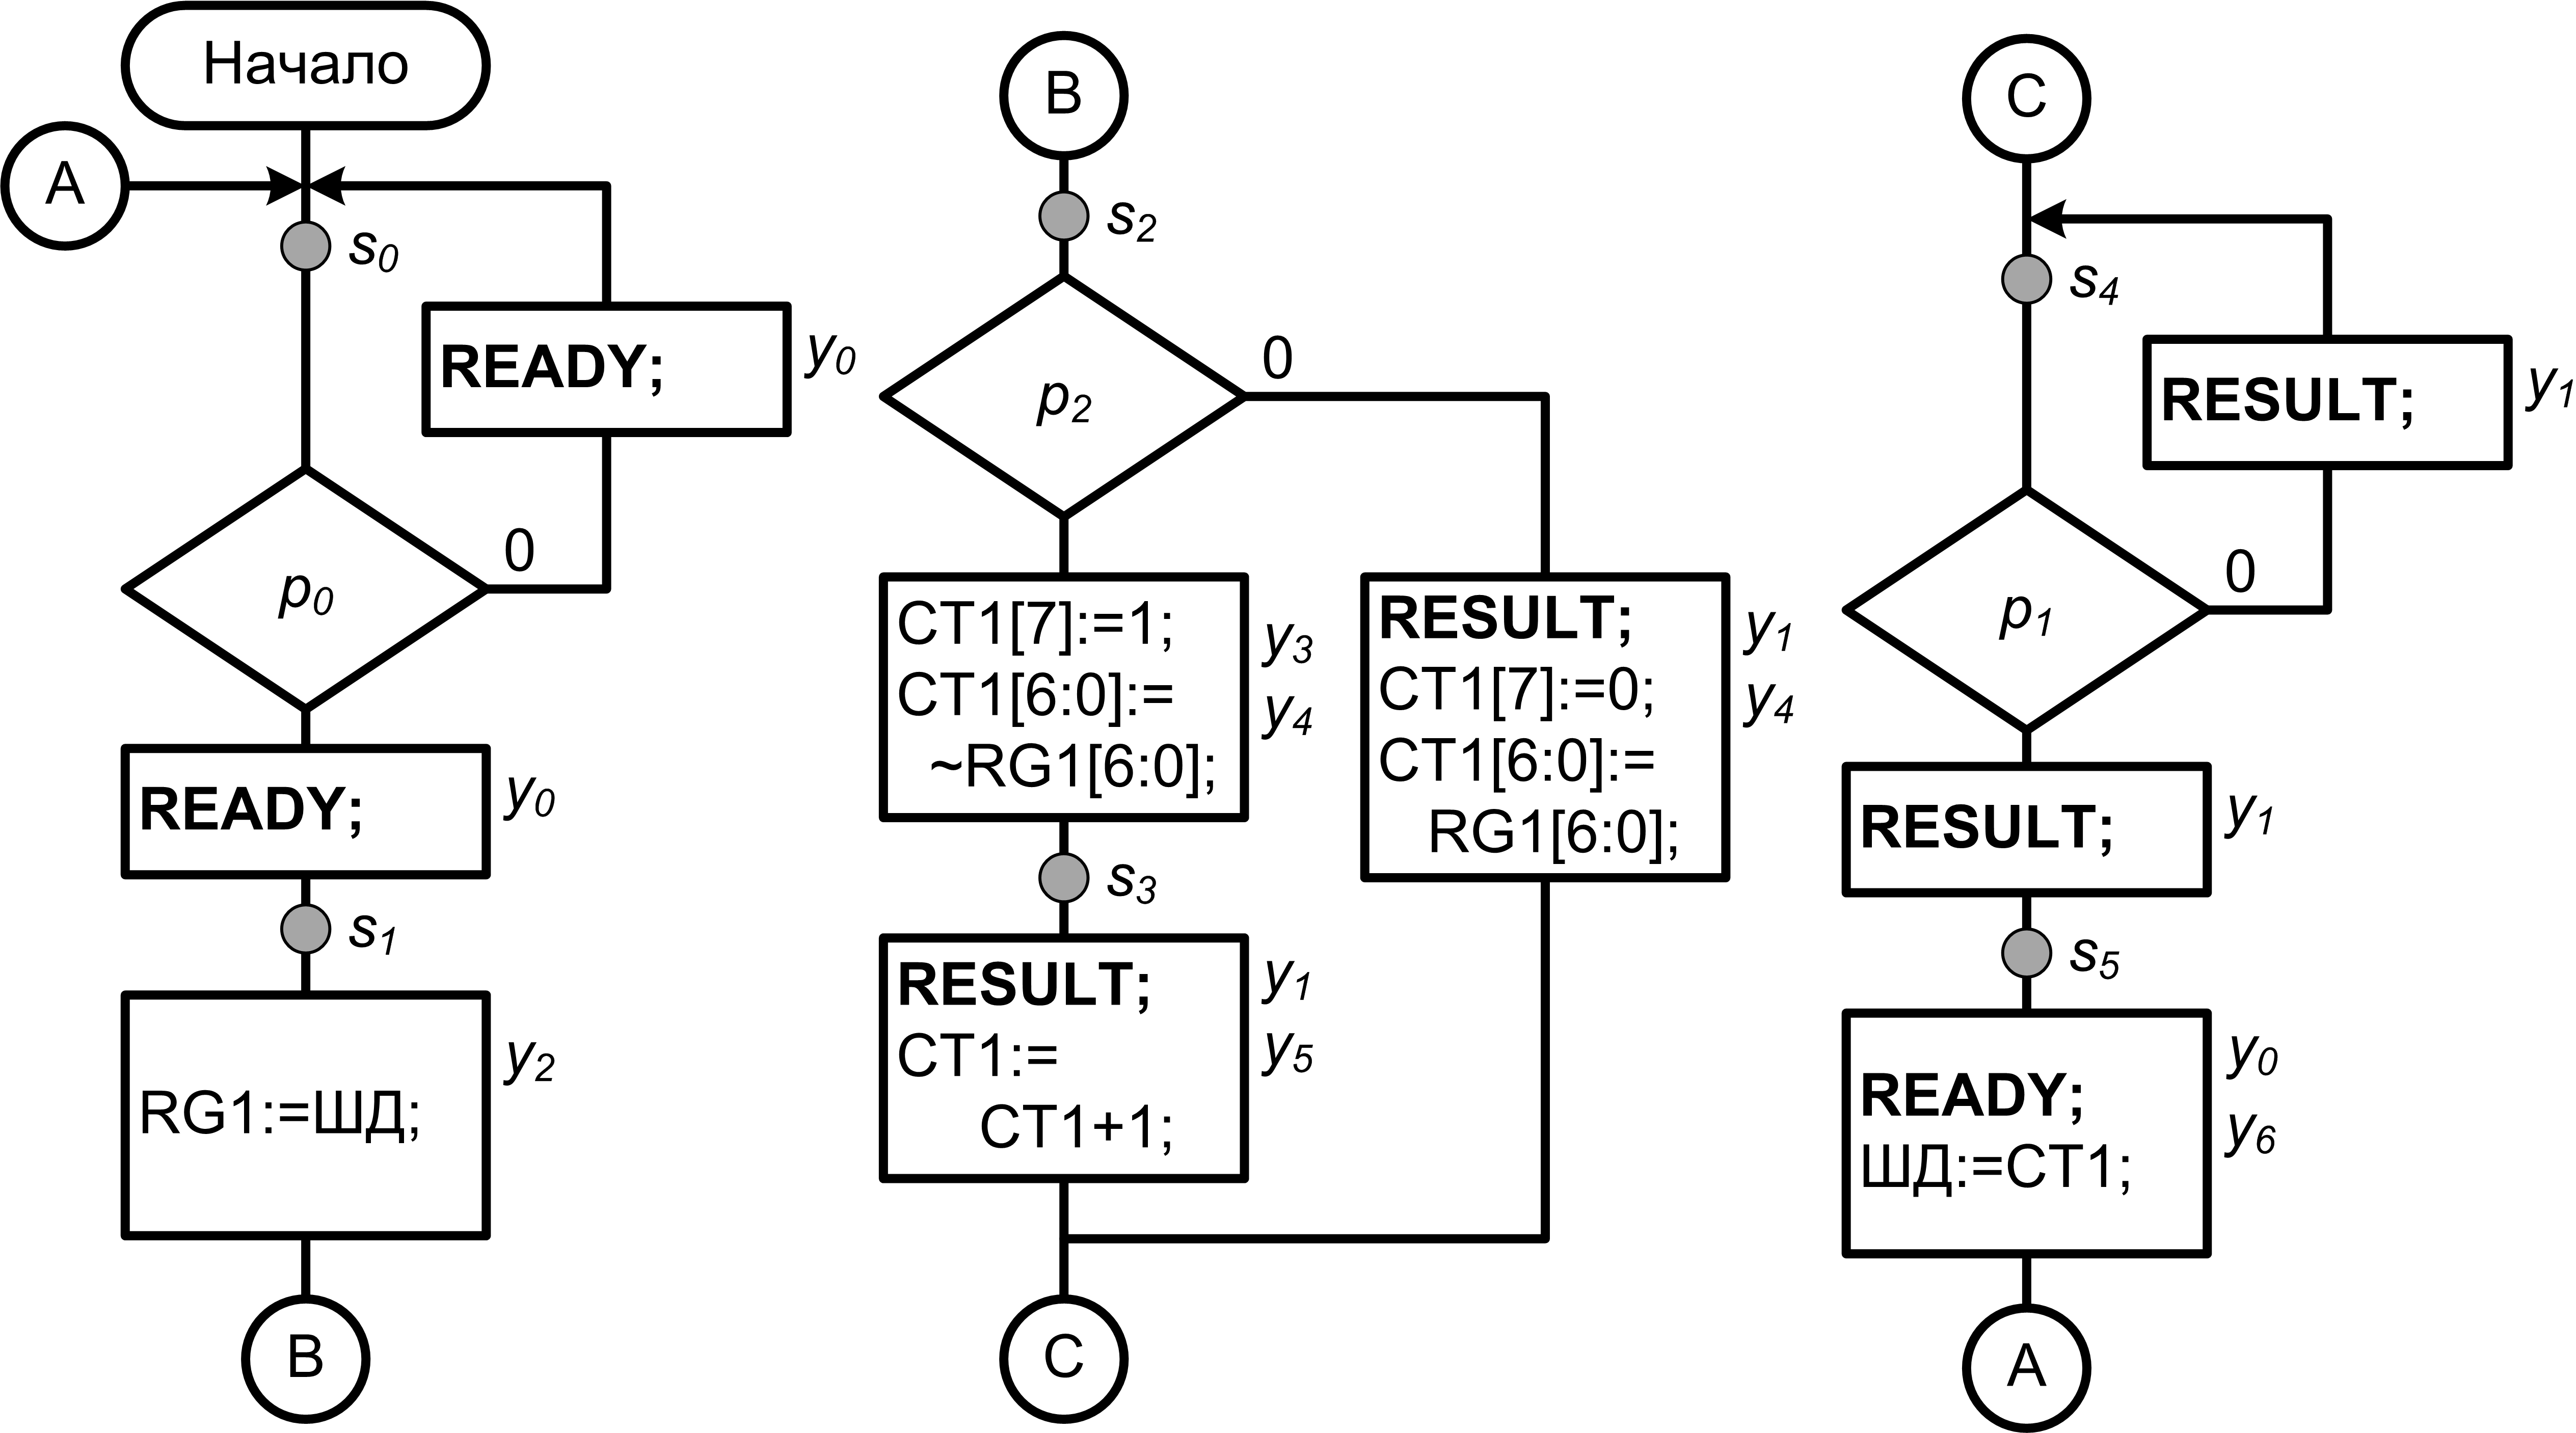
\includegraphics[width=\textwidth]{fig/miliPcDcAlgo}
    \caption{Алгоритм работы преобразователя $\Machine{ПК}\mapsto\Machine{ДК}$ под управлением автомата Мили}
    \label{fig::ch::practice::miliPcDcAlgo}
\end{figure}

Отметка состояния ставится над условной вершиной (см. рисунок \ref{fig::ch::practice::MiliAlg}). При отсутствии таковой, например, между двумя последовательными блоками процеса\footnote{Блок процесса обозначается на блок-схеме прямоугольником}, вводится фиктивная вершина условия с одинаковым исходом для истины и лжи. В данном примере фиктивные условные вершины введены для состояний $s_1$, $s_3$, $s_5$.

Также следует отметить, что сигнал $y_0\Machine{(ACK)}$ (<<Задание принял>>) выдается в следующем такте (при переходе из состояния $s_1$). Автомат мог среагировать на поступивший сигнал $p_0$ в текущем такте и выдать подтверждение приема задания, но это могло привести к гонкам\footnote{Потому что упрвляющий автомат ЦУУ, при поступлении подтверждения приема должен снять сигнал выдачи задания и, если он это сделает в текущем такте, то начнутся гонки сигналов $p_0$ и $y_0$} и нарушению соглашения приема задания, приведенного на рисунке \ref{fig::ch::practice::timingsTr}.

Соответствующая алгоритму диаграмма переходов автомата уже была приведена на рисунке \ref{fig::ch::practice::MiliDiagram}. Теперь несложно задать микропрограмму для автомата (рисунок \ref{fig::ch::practice::miliMcu}). Это можно сделать как по отмеченной граф-схеме, так и по диаграмме переходов.

\begin{figure}[!ht]
    \centering
    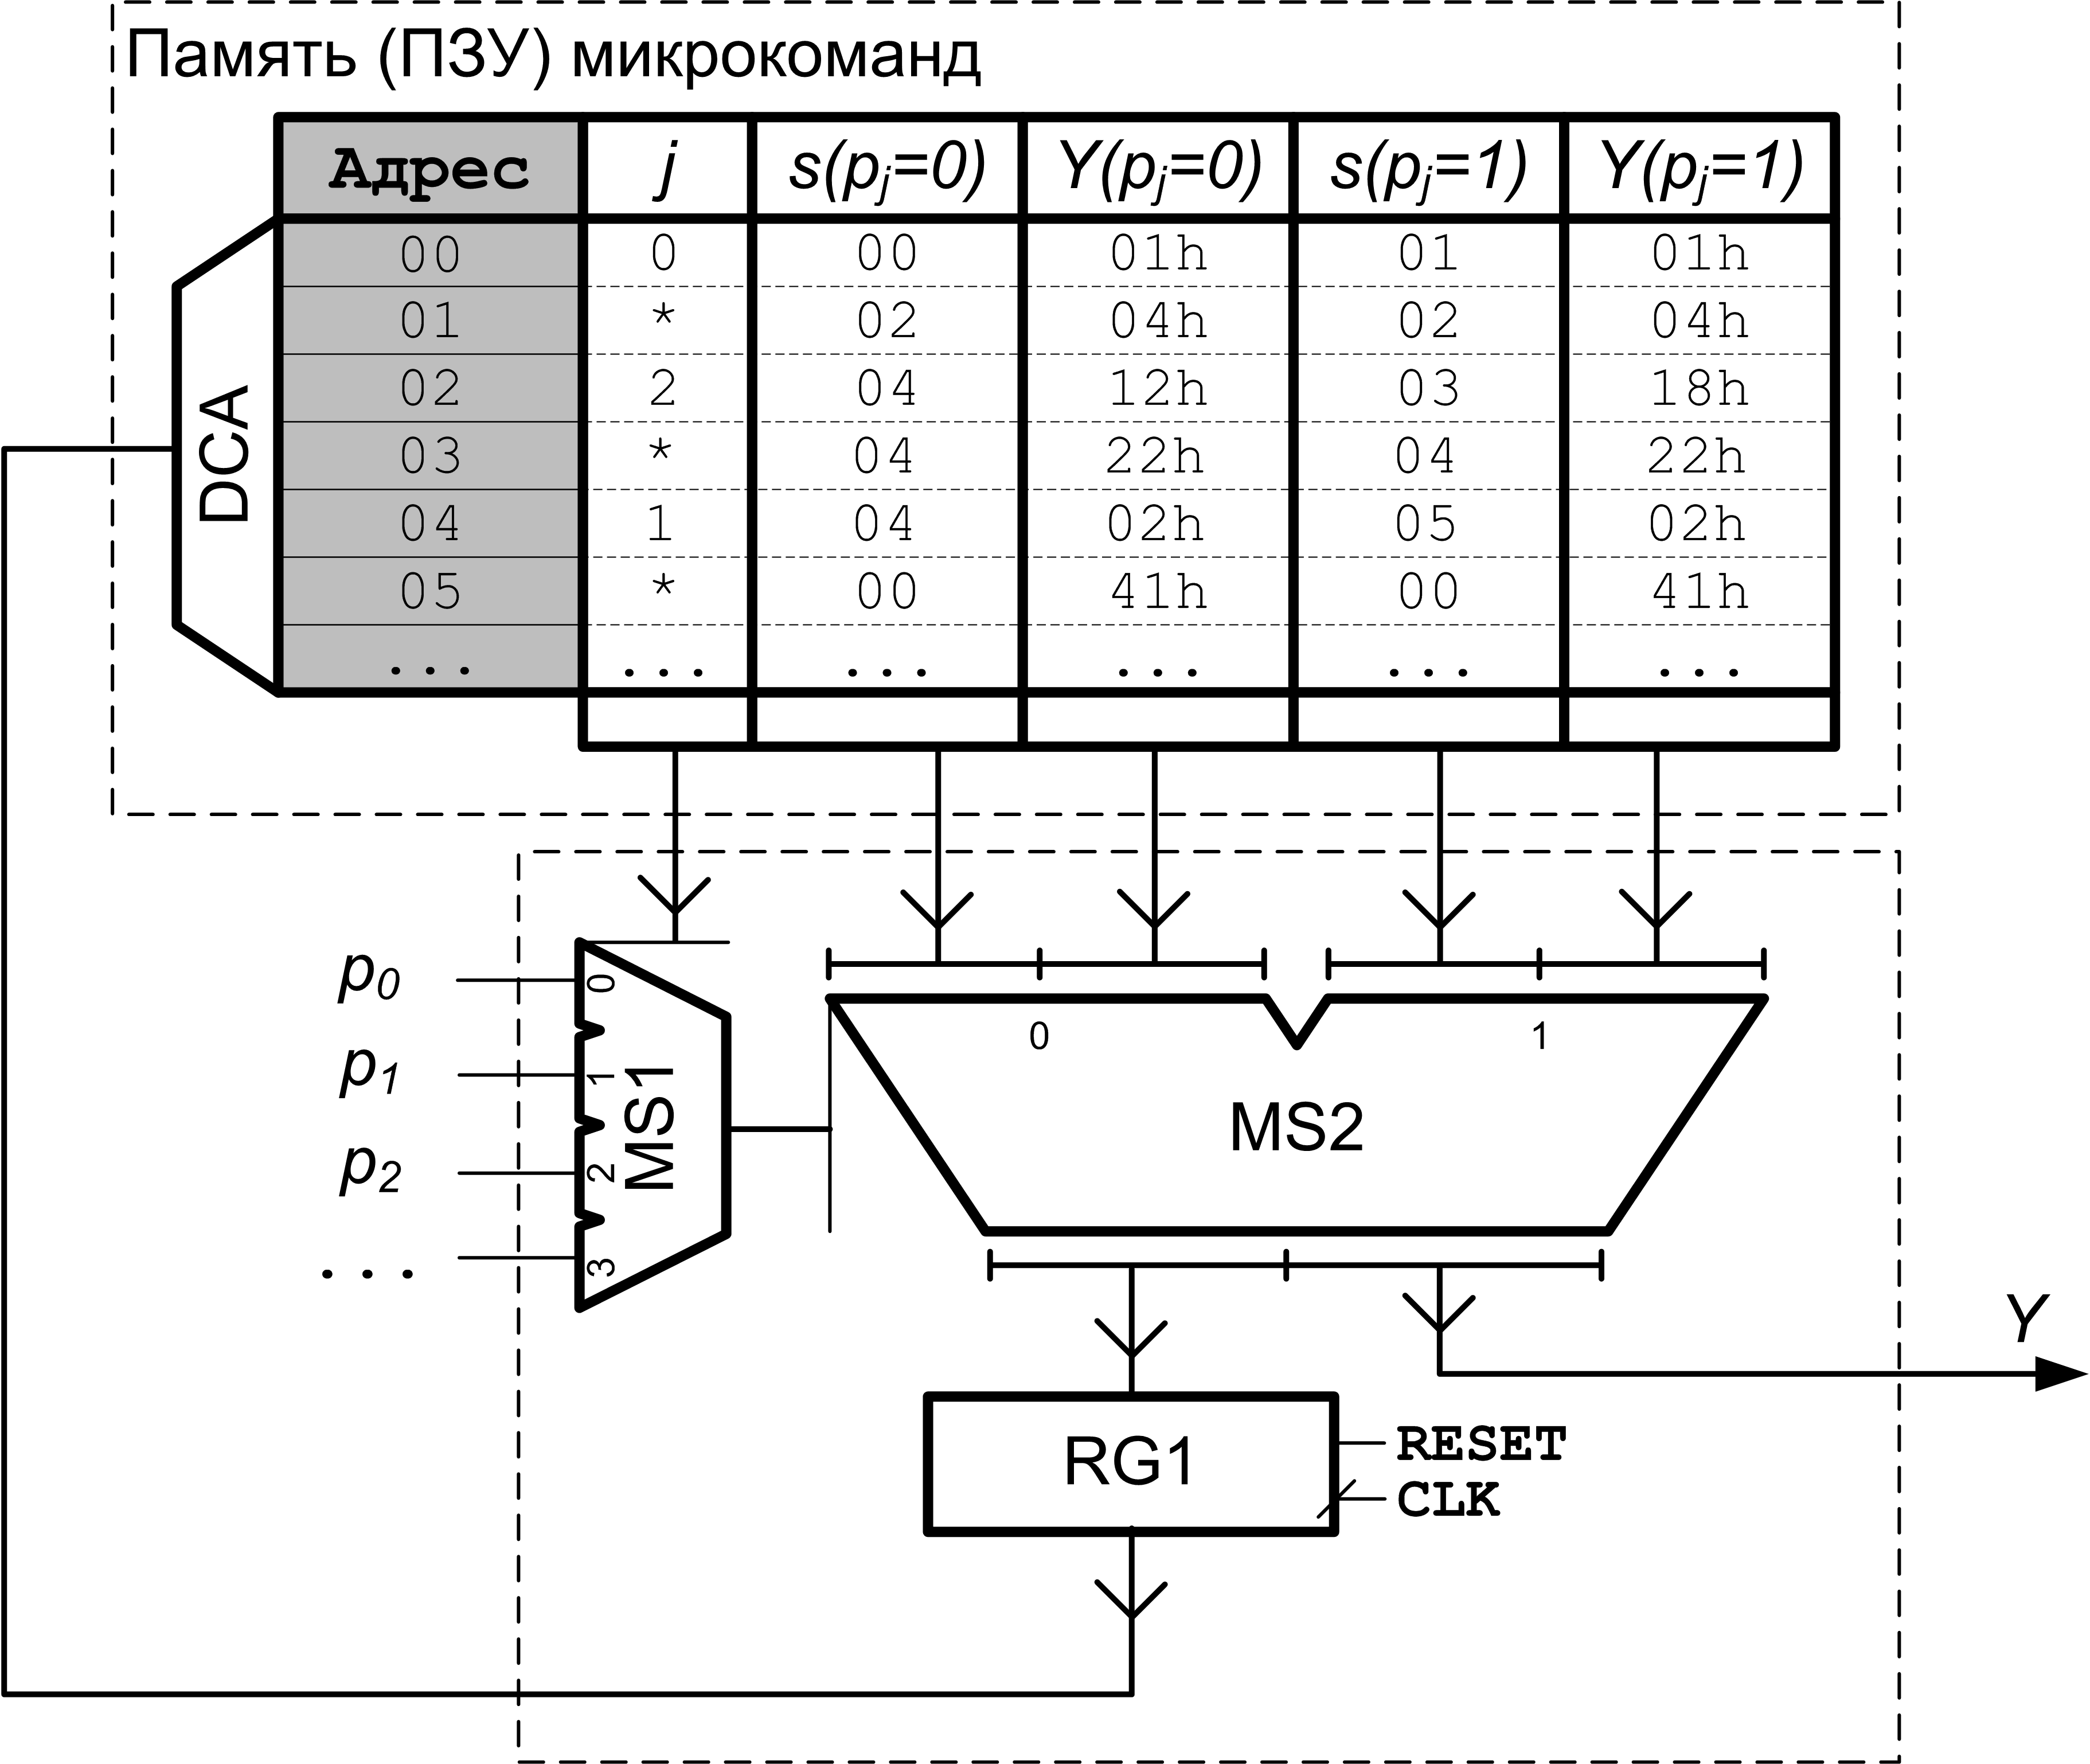
\includegraphics[width=.7\textwidth]{fig/miliMcu}
    \caption{Микропрограмма автомата Мили}
    \label{fig::ch::practice::miliMcu}
\end{figure}

Временная диаграмма работы преобразователя $\Machine{ПК}\mapsto\Machine{ДК}$ под управлением автомата Мили приводится на рисунке \ref{fig::ch::practice::timingsMili}.

\begin{figure}[!ht]
    \centering
    \includegraphics{fig/timings.3}
    \caption{Временная диаграмма работы преобразователя $\Machine{ПК}\mapsto\Machine{ДК}$ под управлением автомата Мили}
    \label{fig::ch::practice::timingsMili}
\end{figure}


\subsubsection{Автомат Мура}

Алгоритм работы преобразователя $\Machine{ПК}\mapsto\Machine{ДК}$, учитывающий особенности управляющего автомата Мура приведен на рисунке \ref{fig::ch::practice::moorePcDcAlgo}.

%todo особенности

\begin{figure}[!ht]
    \centering
    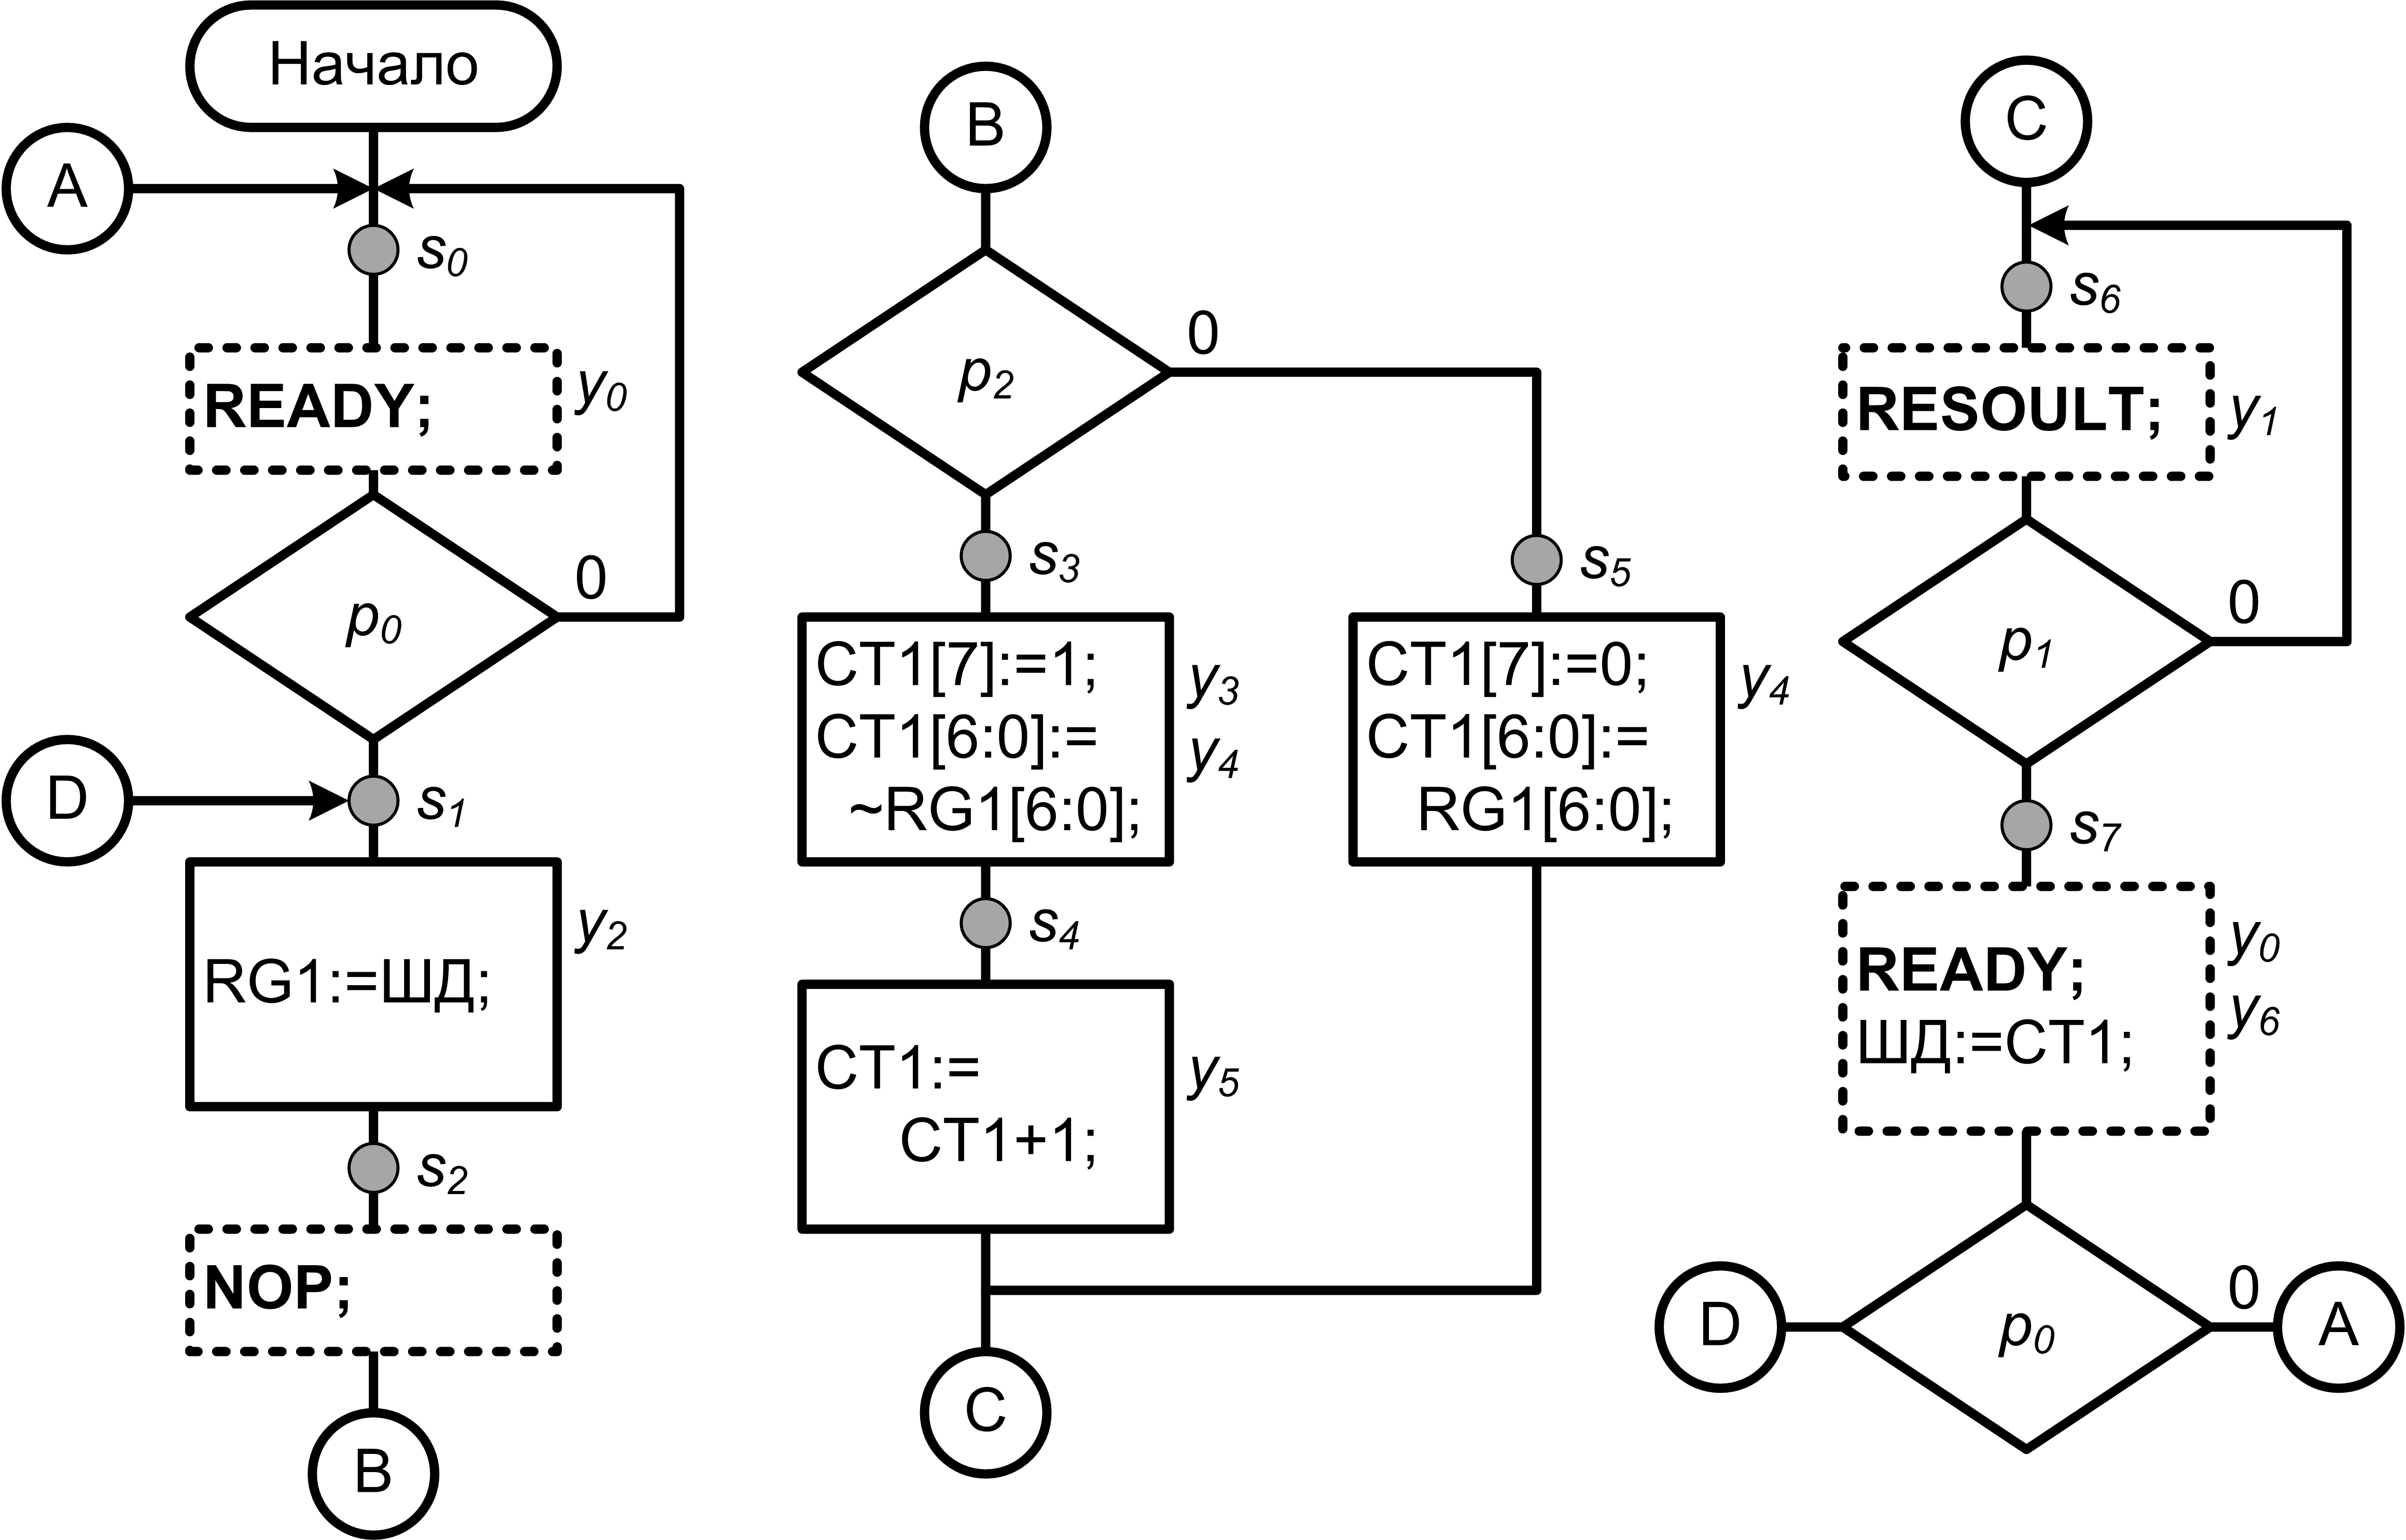
\includegraphics[width=\textwidth]{fig/moorePcDcAlgo}
    \caption{Алгоритм работы преобразователя $\Machine{ПК}\mapsto\Machine{ДК}$ под управлением автомата Мура}
    \label{fig::ch::practice::moorePcDcAlgo}
\end{figure}

Диаграмма состояний автомата Мура уже была приведена на рисунке \ref{fig::ch::practice::MooreDiagram}. Обычно у автомата Мура, эквивалентного автомату Мили, состояний больше, и времени (тактов) на работу он также тратит больше.

Прошивка памяти микропрограммного автомата Мура приводится на рисунке \ref{fig::ch::practice::mooreMcu}.

\begin{figure}[!ht]
    \centering
    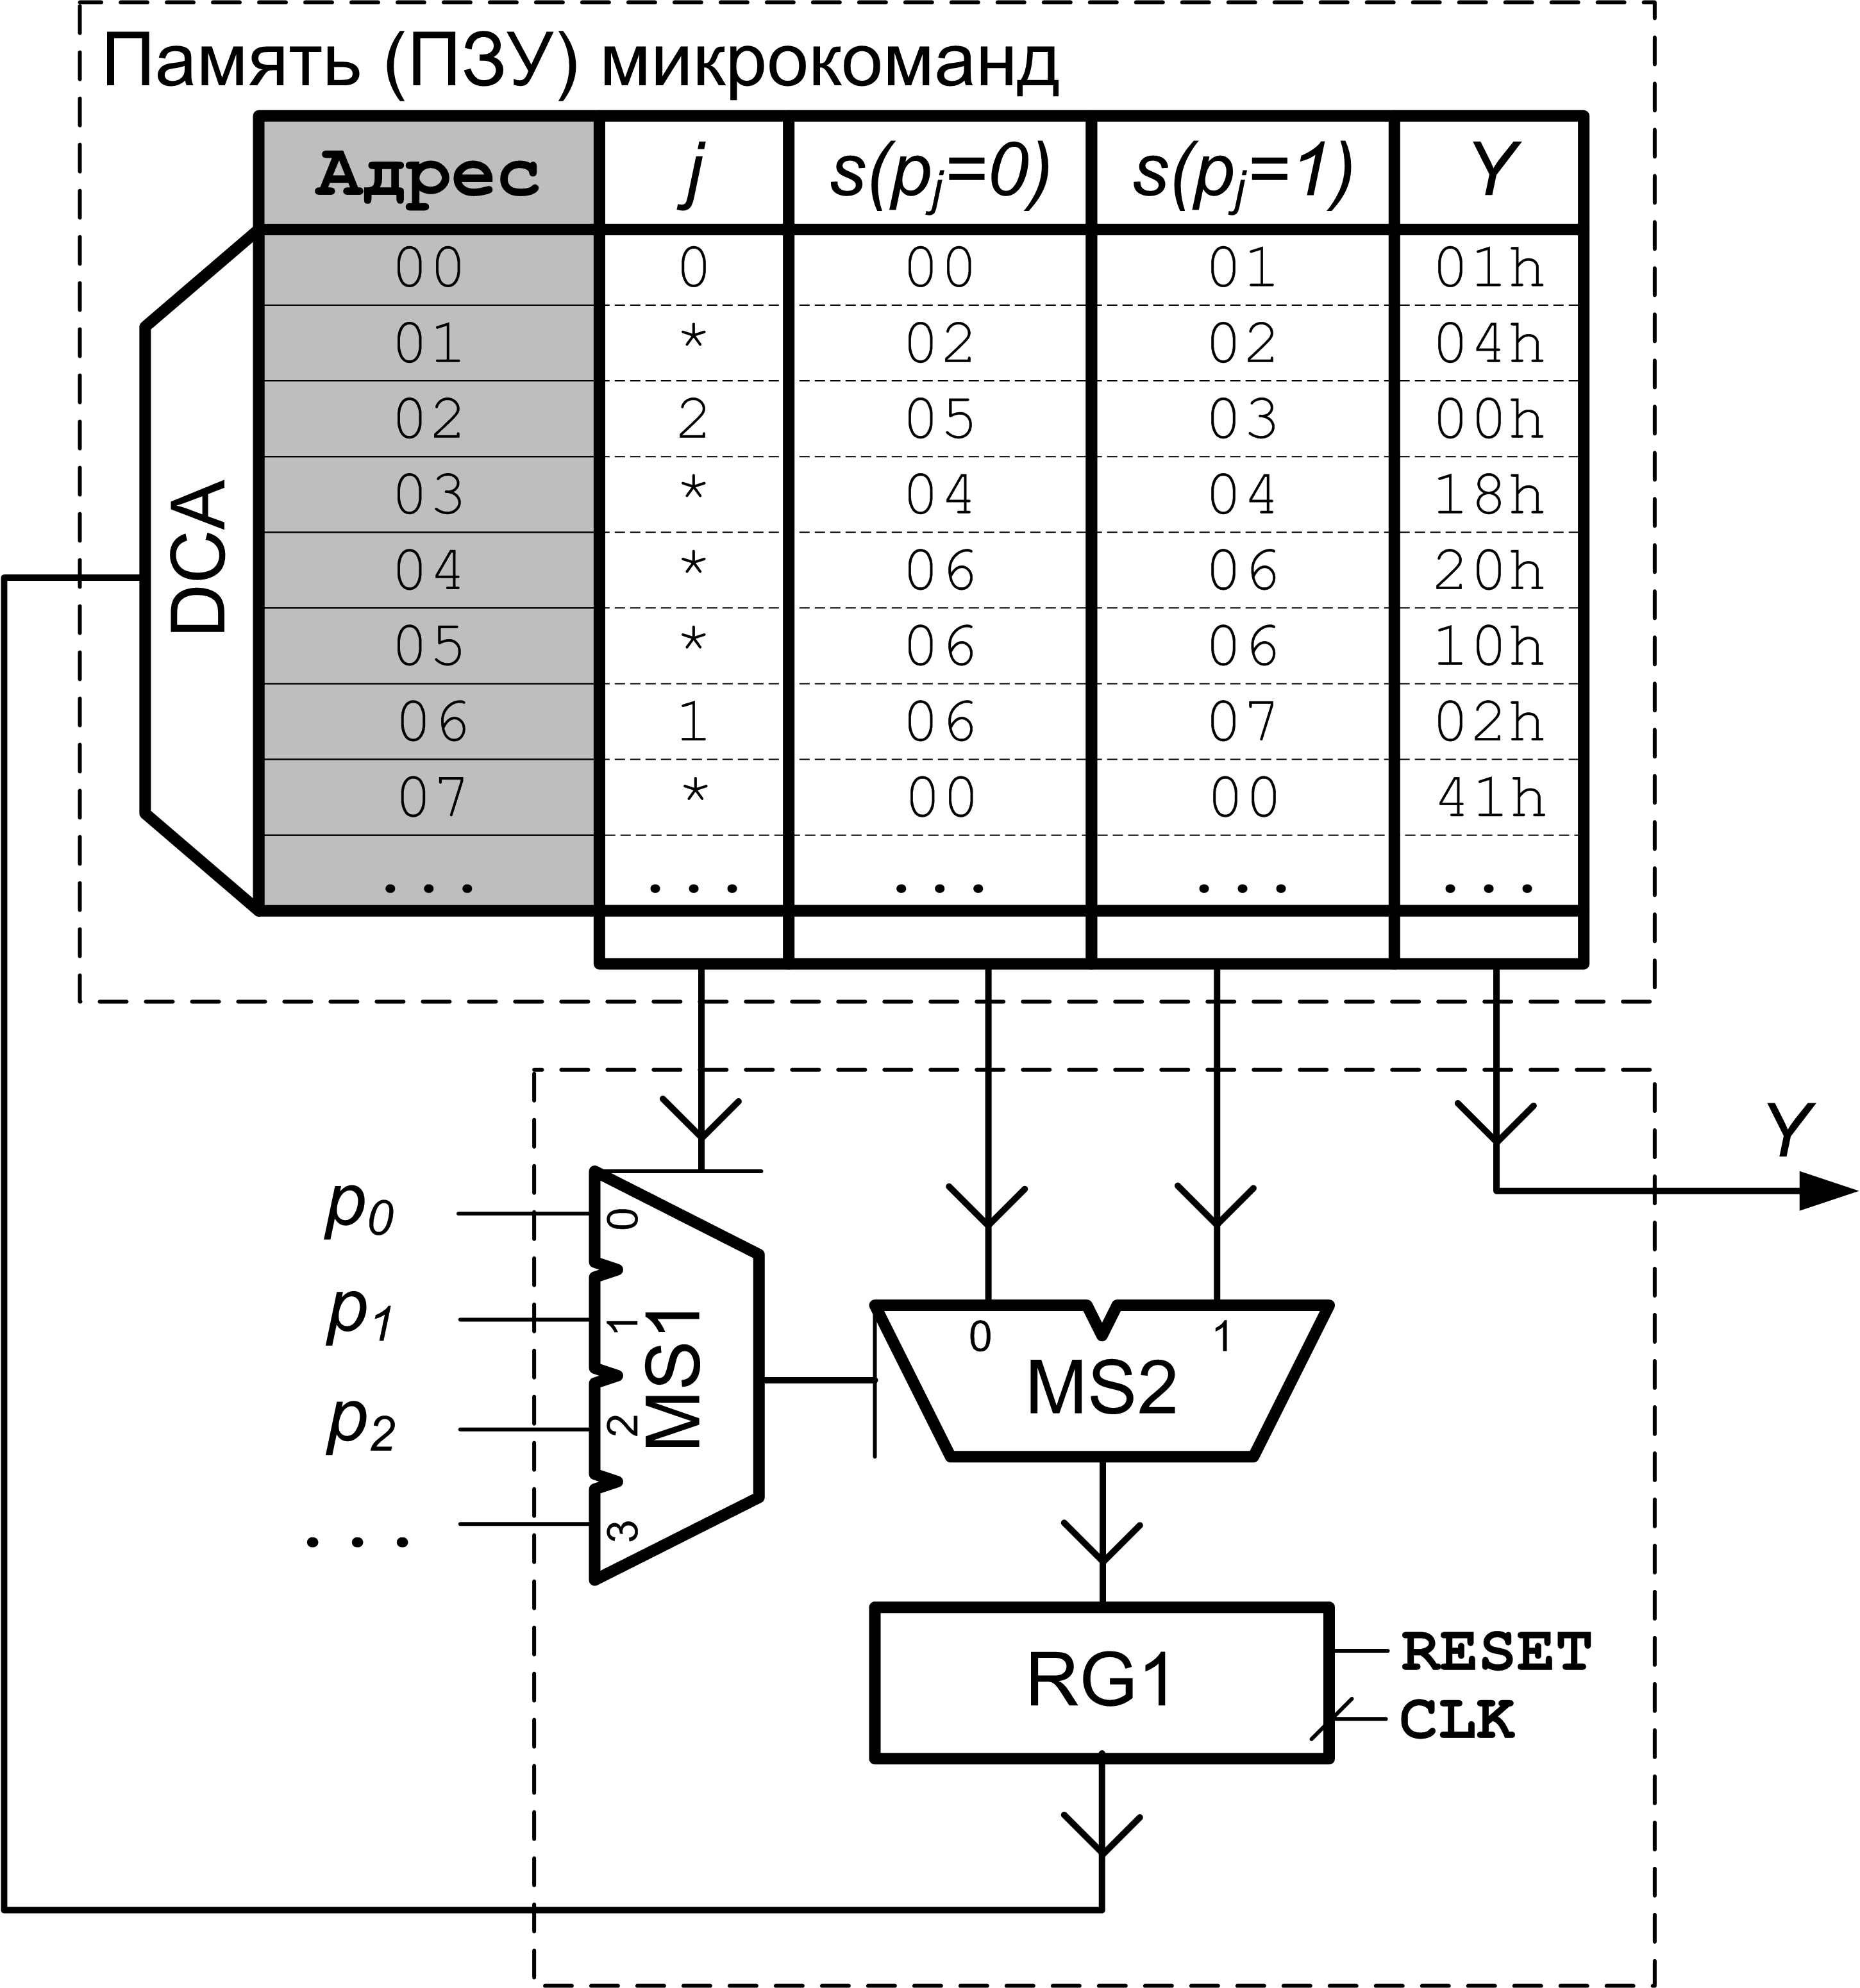
\includegraphics[width=.6\textwidth]{fig/mooreMcu}
    \caption{Микропрограмма автомата Мура}
    \label{fig::ch::practice::mooreMcu}
\end{figure}

Временная диаграмма работы автомата Мура приведена на рисунке \ref{fig::ch::practice::timingsMoore}.

\begin{figure}[!ht]
    \centering
    \includegraphics{fig/timings.4}
    \caption{Временная диаграмма работы преобразователя $\Machine{ПК}\mapsto\Machine{ДК}$ под управлением автомата Мура}
    \label{fig::ch::practice::timingsMoore}
\end{figure}



\section{Работа с лабораторной установкой <<Microcode>>}
\label{s::ch::practice::software}

Цель лабораторной установки <<Microcode>> --- закрепление теоретических основ реализации арифметических операций.

Поставленная цель достигается за счет того, что:
\begin{itemize}
    \item предлагается готовая операционная часть устройства (см. рисунок \ref{fig::ch::practice::model} и теорию в разделе \ref{ch::practice}), в структуре которой требуется разобраться и понять, как имеющимися средствами решить задачу (т.е. выполнить некоторую арифметическую операцию);

    \item моделируется работа центрального управляющего устройства, которое выдает задание и принимает результаты по определенным правилам;

    \item <<Microcode>> позволяет студенту задать собственные входные данные и выполнить пошаговое управление в режиме отладки;
    
    \item <<Microcode>> автоматически выполняет многократное тестирование правильности решения задачи по методу <<черного ящика>>;
    
    \item выполняемые <<Microcode>> тесты покрывают все ветки правильного алгоритма решения задачи (арифметической операции);
    
    \item тесты покрытия создаются <<Microcode>> на основе генератора случайных чисел;
    
    \item в <<Microcode>> заложена возможность генерации индивидуальных вариантов заданий, создаваемых за счет перестановки индексов управляющих сигналов $y$, что порождает $n!$ возможных уникальных вариантов кодирования, при среднем $n\ge 12$;
    
    \item в диалогах <<Microcode>> для ввода отладочных данных автоматически рассчитывается результат, а также выводятся десятичные представления числовых операндов, что дает возмножность глубже разобраться в форматах и кодах.
\end{itemize}


\subsection{Принципы работы <<Microcode>>}

Лабораторная установка <<Microcode>> позволяет загружать групу заданий. Например, в рамках одной группы могут быть загружены задания на умножение чисел различными способами (см. рисунок \ref{fig:mic:MicWindow}).

\begin{figure}
    \centering
    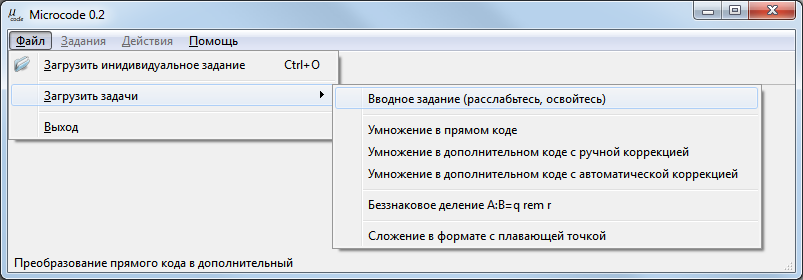
\includegraphics[width=\textwidth]{fig/MicWindow}
    \caption{Главное окно <<Microcode>> (русский язык интерфейса)}\label{fig:mic:MicWindow}
\end{figure}

Отдельное задание представляет собой вычислительное устройство, постороенное в соответствии с принципами, изложенными в разделе \ref{ch::practice} и способное выполнять ту или иную сложную вычислительную операцию, например, умножение или деление.

Пользователю предлагается готовая схема операционной части, в устройстве и назначении которой он должен разобраться, опираясь на изученную теорию. В распоряжении пользователя имеется набор управляющих сигналов, с помощью которых он может изменять состояние операционной части. Задача пользователя --- реализовать алгоритм работы сложной вычислительной операции.

У пользователя имеются следующие возможности реализовать алгоритм работы устройства:
\begin{itemize}
    \item вручную выполнить выдачу необходимых управляющих сигналов, предварительно задав наборы управляющих сигналов в ПЗУ микрокоманд;
    \item запрограммировать автомат Мили или Мура, заполнив таблицу ПЗУ микропрограмм.
\end{itemize}

Все значения в таблицы ПЗУ заносятся в шестнадцатеричной системе счисления. Управляющие сигналы кодируются двоичным вектором, который в ПЗУ вносится в шестнадцатеричном представлении, например, если требуется выдать сигналы $y_5,y_3,y_2,y_0$, то в соответствующей ячейке ПЗУ нужно записать значение \Machine{0x2D}.

По команде пользователя <<Microcode>> выполняет автоматическое тестирование составленного пользователем алгоритма. Чтобы составить корректный алгоритм, пользователь может использовать специальный режим отладки, в котором он может задать исходные данные и в пошаговом режиме отследить изменения, происходящие в операционной части.

Прохождение автоматических тестов является допуском к защите разультатов работы.


\subsection{Задания на лабораторные работы}

В рамках лабораторной работы студент выполняет задание, которое выдает преподаватель.

В лабораторной установке <<Microcode>> реализованы следующие задания: 
\begin{itemize}
    \item перевод прямого кода в дополнительный;
    \item умножение в прямом коде;
    \item умножение в дополнительном коде с ручной коррекцией;
    \item умножение в дополнительном коде с автоматической коррекцией;
    \item беззнаковое деление $A\div B = \DivAnswer{q}{r}$;
    \item сложение в формате с плавающей точкой.
\end{itemize}


\subsection{Выполнение задания}

После выбора группы заданий, становится активным пункт меню <<Задания>>(<<Tasks>>), позволяющий переключаться между заданиями в рамках группы (см. рисунок \ref{fig:mic:MicTaskWindow}). Менять группу заданий в дальнейшем нельзя.

\begin{figure}
    \centering
    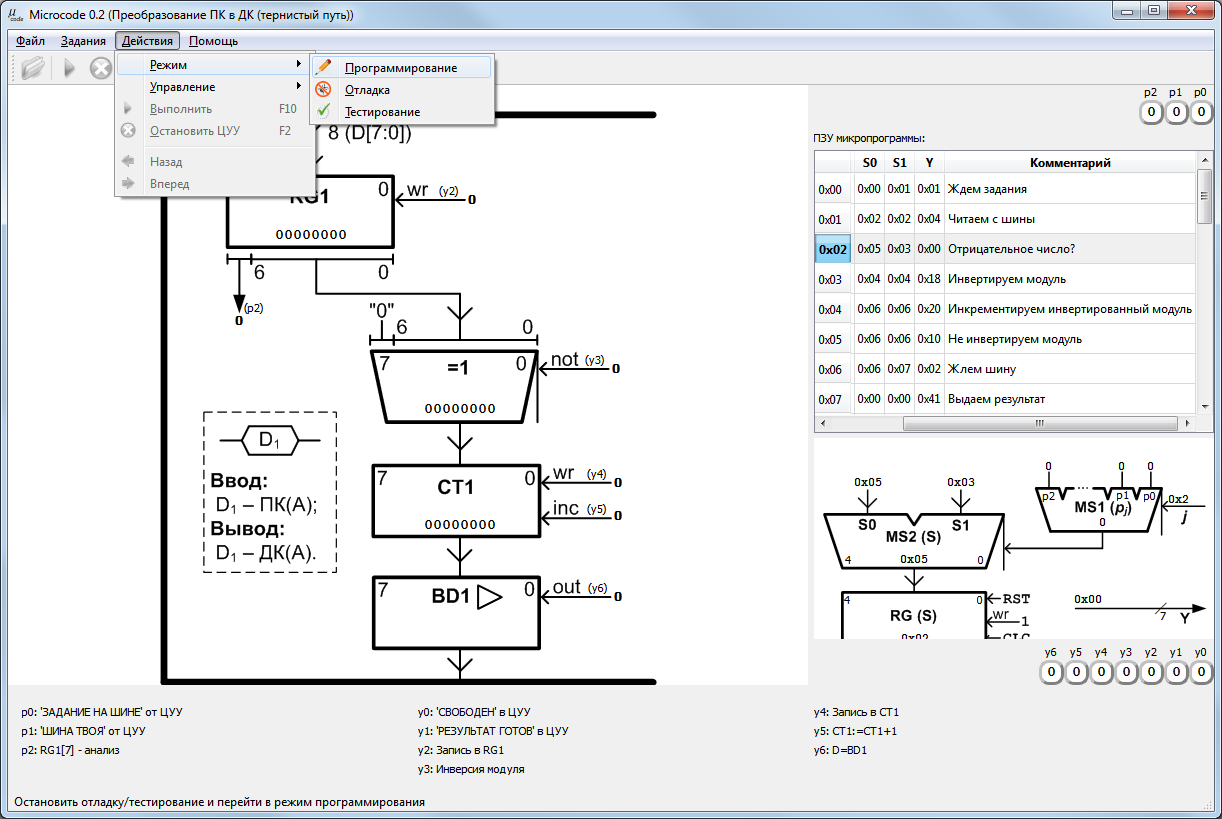
\includegraphics[width=\textwidth]{fig/MicTaskWindow}
    \caption{<<Microcode>> после загрузки заданий}\label{fig:mic:MicTaskWindow}
\end{figure}

Пункт меню <<Действия>> позволяет выполнить те или иные действия в текущем задании:
\begin{itemize}
    \item выбрать один из режимов работы: <<Программирование>> (
\includegraphics[width=16pt]{fig/microcode/image/programming.png}), <<Отладка>> (
\includegraphics[width=16pt]{fig/microcode/image/debug.png}) или <<Тестирование>> (
\includegraphics[width=16pt]{fig/microcode/image/autotest.png});
    \item выбрать управление: <<Ручное>> (
\includegraphics[width=16pt]{fig/microcode/image/manualgun.png}), 
                              <<Автомат Мили>> (\includegraphics[width=16pt]{fig/microcode/image/miligun.png})
                              или <<Автомат Мура>> (\includegraphics[width=16pt]{fig/microcode/image/mooregun.png});
    \item выполнять/останавливать шаги отладки или автотесты;
    \item перемещаться в отладочном режиме по истории тактов.
\end{itemize}

Режим работы <<Программирование>> (<<Programming>>) предназначен для редактирования ПЗУ управляющей части. Как только редактирование ячейки ПЗУ завершается, соответствующие управляющие сигналы распространаяются по схеме, но ошибки управления не выдаются, даже если они есть.

Режим <<Отладка>> (<<Debug>>) предназначен для пошагового выполнения придуманного студентом алгоритма управления. В момент переключения в этот режим студенту предлагается ввести исходные данные. После того, как данные будут введены, <<Microcode>> переключается в пошаговый (потактный) режим тестирования. В случае ручного управления (<<Управление/Ручное>> (<<MCU/Manual>>)) пользователь выбирает в таблице <<ПЗУ микрокоманд>> строку с нужной командой и нажимает кнопку <<Выполнить>> (<<Execute>>) или горячую клавишу <<F10>>, что приводит к переключению в следующий такт. В случае автоматического управления (<<Aвтомат Мили>> (<<Mili>>), <<Автомат Мура>> (<<Moore>>)) текущая ячейка ПЗУ микропрограммы (строка таблицы) подсвечивается. Если в процессе выполнения теста фиксируется ошибка, то тестирование прекращается, выводится соответствующее сообщение, и выполняется переход в режим программирования. Если алгоритм выполнен безошибочно и в ЦУУ корректно выдан правильный результат, то выводится информационное сообщение об успешном прохождении отладочного теста.

В режиме <<Тестирование>> (<<Autotest>>) выполняется тестирование на случайным образом генерируемых входных данных. Состояние операционной части при этом не отображается. При ручном управлении автотесты выполняются в пошаговом режиме, в противном случае --- в автоматическом.

В режимах отладки и тестирования фиксируются следующие ошибки, приводящие к прекращению теста:
\begin{itemize}
    \item выполняется чтение данных с <<пустой>> шины;
    \item выполняется выдача данных на <<занятую>> шину;
    \item нарушается протокол взаимодействия с ЦУУ, например, до выдачи результата, выдается сигнал <<Свободен>>;
    \item выдаются конфликтующие сигналы управления элементом памяти, например на регистр одновременно подаются управляющие сигналы сдвига и сброса.
\end{itemize}

Чтобы считать операнды, требуется выполнить следующие действия.
\begin{itemize}
    \item Выдавать сигнал <<Свободен>> ($y_0$, $Y=\Machine{0x0001}$) в течение некоторого числа тактов (не более 6), пока осведомительный сигнал <<Задание на шине>> ($p_0$) не установится в 1.
    \item Сигнал <<Задание на шине>> выдается ЦУУ в течение одного такта, в этом такте также нужно выдавать сигнал <<Свободен>>.
    \item ЦУУ, в течение одного или нескольких тактов, следующих после такта, в котором выдавался сигнал <<Задание на шине>> выдает на шину фрагменты задания. Необходимо считать эти фрагменты в регистры.
\end{itemize}

Чтобы выдать результат, требуется выполнить следующие действия.
\begin{itemize}
    \item Выдавать сигнал <<Результат готов>> ($y_1$, $Y=\Machine{0x0002}$) в течение некоторого числа тактов (не более 6), пока осведомительный сигнал <<Шина твоя>> ($p_0$) не установится в 1.
    \item Сигнал <<Шина твоя>> выдается ЦУУ в течение одного такта, в этом такте также нужно выдавать сигнал <<Результат готов>>.
    \item В течение одного или нескольких тактов, следующих после такта, в котором выдавался сигнал <<Шина твоя>> следует в определенном в задании порядке выдавать фрагменты результата на шину.
\end{itemize}


Результатом работы являются заполненные ПЗУ микрокоманд (ПЗУ микропрограмм). Допуском к защите результатов работы является успешное прохождение студентом отладочных или автоматических тестов.


\subsection{Генерация индивидуальных вариантов заданий}

С помощью microcode можно сгенерировать индивидуальные варианты для каждого студента. Для этих целей нужно сформировать специальный текстовый файл, содержащий список адресатов\footnote{Тех, для кого предназначены индивидуальные варианты заданий. Т.е. студентов.} в формате JSON\footnote{JSON --- JavaScript Object Notation.  Текстовый формат обмена данными, основанный на JavaScript. Прост и лаконичен. Как и многие другие текстовые форматы, JSON легко читается людьми. Формат был разработан Дугласом Крокфордом.}. Файл должен быть сохранен в кодировке UTF-8 и может быть создан в любом подходящем текстовом редакторе.

JSON-содержимое файла адресатов представляет собой массив объектов, состоящих из двух строковых атрибутов:
\begin{itemize}
    \item \verb"id" --- строка, идентифицирующая студента, как правило, содержащая Ф.И.О. студента;
    \item \verb"secret_prefix" --- секретная информация\footnote{В зависимости от степени параноидальности преподавателя, может быть как случайной последовательностью, так и вполне предсказуемой по некоторому, известному только преподавателю, правилу, например, фамилия студента на латинице, или его Ф.И.О., или первые три буквы фамилии\ldots}.
\end{itemize}

Пример содержимого файла адресатов:
\begin{verbatim}
[
    {   "id": "Иванов И.И.",
        "secret_prefix": "IvanovSecret"},
        
    {   "id": "Петров П.П.",
        "secret_prefix": "PetrovSecret"},
        
    {   "id": "Сидоров С.С.",
        "secret_prefix": "SidorovSecret"}
]
\end{verbatim}

После того, как файл подготовлен, можно сгенерировать с помощью microcode индивидуальные варианты. Для этого выполняется пункт меню <<Файл/Создать индивидуальные варианты\ldots>> (<<File/Create individual vatiants\ldots>>). В появившемся диалоге (см. рисунок \ref{fig:mic:genvariants}) следует заполнить необходимые поля.
\begin{itemize}
    \item <<Секрет>>(<<The secret:>>) --- секретная информация, которая используется для проверки подлинности индивидуального варианта. Описание проверки подлинности приводится в разделе \ref{ss:mic:check}.
    
    \item <<Файл с адресатами:>>(<<The recipients file:>>) --- путь к подготовленному файлу адресатов.
    
    \item <<Варианты в папку:>>(<<Variants folder:>>) --- каталог, в котором будут созданы файлы индивидуальных вариантов. Имена файлов будут совпадать со значением атрибута \verb"id" в файле адресатов и иметь расширение <<*.json>>.
\end{itemize}

\begin{figure}[!ht]
    \centering
    \includegraphics{fig/micvariants}
    \caption{Диалог <<Microcode>> для генерации индивидуальных вариантов (русский язык интерфейса)}\label{fig:mic:genvariants}
\end{figure}

Например, если загрузить приведенный выше файл адресатов, и в качестве секрета ввести <<123>>, то для Иванова будет сгенерирован текстовый файл <<Иванов И.И..json>> со следующим JSON-содержимым:

\begin{verbatim}
{
  "id": "Иванов И.И.",
  "signature": "673e420b...8e76eff8",
  "swap_history": "783590fc...e1c54474"
}
\end{verbatim}

Этот файл может быть загружен в microcode и управляющие сигналы будут перетасованы.


\subsection{Загрузка индивидуального варианта}

После того, как файлы индивидуальных заданий сгенерированы их следует раздать студентам. Индивидуальный вариант загружается студентом командой меню <<Файл/Открыть индивидуальный вариант\ldots>>(<<File/Open individual variant\ldots>>).


\subsection{Проверка подлинности индивидуального варианта}
\label{ss:mic:check}

Файл индивидуального варианта защищен криптографически. Чтобы выполнить проверку подлинности варианта, необходимо выполнить команду меню <<Файл/Проверить индивидуальный вариант\ldots>>(<<File/Validate individual variant\ldots>>).

В диалоге проверки варианта (см. рисунок \ref{fig:mic:checkvarian}) следует ввести конкатенацию секретов $s_1s_2$, где $s_1$ --- секрет, указанный в поле \verb"secret_prefix" файла адресатов, а $s_2$ --- секрет, заданный в диалоге генерации вариантов (см. рисунок \ref{fig:mic:genvariants}).

Для Иванова в приводимых примерах следует ввести: <<IvanovSecret123>>.

\begin{figure}[!ht]
    \centering
    \includegraphics{fig/checkvarian}
    \caption{Диалог <<Microcode>> для проверки подлинности индивидуального варианта (русский язык интерфейса)}\label{fig:mic:checkvarian}
\end{figure}

Без знания секрета, разделенного на две части --- персональную и общую, подделка задания представляет собой вычислительно сложную задачу.

\subsection{Защита результатов работы}

Результаты работы оформляются в виде отчета, в котором для каждого задания необходимо представить:
\begin{itemize}
    \item Таблицы заполненных ПЗУ с построчными комментариями.
    \item Алгоритмы работы управляющего устройства, представленные в виде блок-схемы. Напротив каждого блока процесса должны быть указаны выдаваемые управляющие сигналы.
    \item Таблицы, отражающие пошаговое (потактное) выполнение алгоритма на примере конкретных входных значений.
    \item Выводы в формате формулы изобретения\footnote{Формула изобретения состоит из ограничительной (описательной) и отличительной частей и имеет типовую структуру: <<Изобретение X, состоящее из (список составляющих элементов), отличается тем, что (список отличительных признаков и особенностей)>>. Например, устройство умножения первым способом в прямом коде, реализованное на основе\ldots, отличается тем, что\ldots}. 
    \item Предложения по оптимизации операционной части или микропрограммы.
\end{itemize}

Защищая результаты своей работы, студент должен
\begin{itemize}
    \item \emph{знать}:
    \begin{itemize}
        \item теоретические основы реализуемой в задании вычислительной операции,
        \item принципы работы всех элементов схемы операционной части вычислительного устройства,
        \item протоколы обмена данными с центральным управляющим устройством: <<получение задания>> и <<выдача результата>>;
    \end{itemize}
    \item \emph{уметь}: 
    \begin{itemize}
        \item объяснить, как на предложенной схеме можно реализовать вычислительную операцию (например, в задании умножения в дополнительном коде с ручной коррекцией, указать какие сигналы, в какой последовательности подать, чтобы выполнить коррекцию псевдопроизведения множителем),
        \item кодировать двоичные векторы управляющих сигналов,
        \item реализовать алгоритм вычислительной операции, составляя необходимые наборы микрокоманд или реализуя  микропрограмму,
        \item оценить время выполнения микропрограммы в тактах в зависимости от аргументов: минимальное время, максимальное время, среднее время;
    \end{itemize}
    \item \emph{владеть навыками}:
    \begin{itemize}
        \item перевода двоичных чисел в шестнадцатеричную систему счисления, 
        \item представления чисел в различных форматах, 
        \item составления микропрограмм для автоматов Мили и Мура, 
        \item работы в лабораторной установке <<Microcode>>. 
    \end{itemize}
\end{itemize}


     %практикум
    \chapter{Программирование <<RISC>> --- цикл лабораторных работ}

Лабораторные работы по информатике посвящены арифметическим основам вычислительной техники, т.е. методам обработки символьных представлений чисел.

Указанная обработка выполняется с помощью специального RISC-процессора. RISC (reduced instruction set computing) processor --- процессор с минималистичным набором команд. Современные процессоры с избыточным набором команд, CISC\footnote{CISC --- Complex Instruction Set Computing}, в подавляющем большинстве случаев в своей основе имеют RISC-ядро. При этом сложные команды CISC-процссора реализуются подпрограммами для RISC-ядра. Таким образом, если вдруг обнаруживается ошибка в работе процессора, то её можно исправить обновлением \emph{программного обеспечения процессорного ядра}.
    
Для интерактивного проведения лабораторных работ были разработаны:
\begin{itemize}
    \item архитектура специального процессора с минималистичным набором команд\footnote{RISC --- Reduced Instruction Set Computing}, которая далее сокращенно обозначается \MyProc.
    
    \item программная модель, позволяющая создавать и отлаживать программы на языке ассемблера \MyProc.
    
    \item набор заданий, сводящийся к реализации того или иного алгоритма сложения или умножения чисел на языке ассемблера \MyProc.
\end{itemize}

Выполнение лабораторных работ позволяет студенту:
\begin{itemize}
    \item глубже понять алгоритмы работы сложных операций (умножение, деление) машинной арифметики;
    
    \item разобраться с форматами представления чисел;
    
    \item получить навыки пограммирования при ограниченных вычислительных ресурсах;
    
    \item закрепить основы логики в силу необходимости использования арифметико-логических команд для преобразования на уровне отдельных бит;
    
    \item получить навыки использования двоичной, восьмеричной и шестнадцатеричной систем счисления;
    
    \item освоить техники низкоуровневной оптимизации программ.
\end{itemize}

Классическими трудами по программированию считаются \cite{bib:knuth:artOfProgramming1,bib:knuth:artOfProgramming2,bib:knuth:artOfProgramming3}. Дональдом Кнутом, автором этих трудов, выбран подход к обучению программированию, в основе которого лежит язык ассемблера условной вычислительной машины --- MIX. Несмотря на наличие языков высокого уровня и различных высокоуровневых псеводкодов, Дональд Кнут рекомендует начинать обучение программированию с низкого уровня, а именно с языка ассемблера.

Архитектуру MIX нельзя признать простой --- её автор преследовал цели максимально компактного представления самых разных алгоритмов, которые обсуждались в его работах. В дальнейшем автором была предложена архитектура XMIX --- RISC-версия MIX. Как MIX, так и XMIX не привязаны к двоичной системе счисления.

В данном цикле лабораторных работ используется крайне минималистичная учебная архитектура \MyProc. Цели её создания: возможность работы на уровне бит и возможность реализовать рассмотренные в \cite{bib:lisikov:automateBase,bib:saveliev:automateTheory,bib:fadeeva:vmbase,bib:fadeeva:addmul} алгоритмы машинной арифметики. Также, с целью повысить качество обучения было принято решение сделать динамический выбор базисного набора RISC-команд, что позволит свести к минимуму плагиат и даст студентам возможность научиться решать задачи крайне ограниченным набором средств.
    
\section{Архитектура RISC-процессора \MyProc}
\label{ch::risc}


Преимущества RISC-архитектур в быстроте освоения програмистом, а недостатки заключаются в необходимости реализовать относительно простые операции нетривиальными подпрограммами или макроподстановками. Особенности работы с RISC исчерпывающе изложены в \cite{bib:warren:algTriks}.

\subsection{Память и адресные пространства \MyProc}

В процессоре \MyProc:
\begin{itemize}
    \item имеется 8 байтовых (8-и битных) регистров \Machine{r0},\Machine{r1},\ldots,\Machine{r7};
    \item доступна память данных из 256 8-битных ячеек с адресами от 0 до 255;
    \item оступен единственный порт ввода 8-и битного числа (см. описание команды \Opcode{in});
    \item доступен единственный порт вывода 8-и битного числа, (см. описание команды \Opcode{out});
    \item обращение к ячейке памяти данных возможно двумя способами:
    \begin{itemize}
        \item непосредственная адресация, например, <<\Machine{[0]}>> --- обращение к нулевой ячейке памяти;
        \item регистровая адресация, например, <<\Machine{[r1]}>> --- обращение к ячейке памяти с адресом, значение которого берется из регистра \Machine{r1}. Использовать для обращения к памяти можно любой из 8-и регистров.
    \end{itemize}
\end{itemize}


\subsection{Система команд \MyProc}

Архитектура {\MyProc} позволяет пользователю выбрать набор базисных команд из полного набора. Это на практике позволяет предоставить каждому студенту индивидуальный набор базисных команд. Принципы построения базисного набора инструкций изложены ниже. Полный набор команд следующий:

\begin{itemize}
    \item <<\CmdOneAddr{in}{приемник}>>. Команда ввода байта из порта ввода в \Operand{приемник}. При выполнении этой команды в программной модели {\MyProc} пользователю предлагается ввести число с экрана, которое затем заносится в \Operand{приемник}.
    
    \item <<\CmdOneAddr{out}{источник}>>. Команда записи в порт вывода. При выполнении этой команды в программной модели {\MyProc} значение байта \Operand{источник} выводится на экран.
    
    \item <<\CmdThreeAddr{ror}{источник}{количество-разрядов}{приемник}>>. Команда циклического сдвига вправо на заданное количество разрядов. \Operand{источник} циклически сдвигается на \Operand{количество-разрядов} вправо и результат сдвига записывается в \Operand{приемник}.
    
    \item <<\CmdThreeAddr{rol}{источник}{количество-разрядов}{приемник}>>. Команда циклического сдвига влево на заданное количество разрядов. \Operand{источник} циклически сдвигается на \Operand{количество-разрядов} влево и результат сдвига записывается в \Operand{приемник}.
    
    \item <<\CmdTwoAddr{not}{источник}{приемник}>>. Поразрядное логическое НЕ. Все разряды байта \Operand{источник} инвертиурются и результат записыается в \Operand{приемник}.
    
    \item <<\CmdThreeAddr{or}{источник1}{источник2}{приемник}>>. Поразрядное логическое ИЛИ. 
        \[
            \Operand{приемник} \gets \Operand{источник1} \lor \Operand{источник2}.
        \]
    
    \item <<\CmdThreeAddr{and}{источник1}{источник2}{приемник}>>. Поразрядное логическое И.
    \item <<\CmdThreeAddr{nor}{источник1}{источник2}{приемник}>>.  Поразрядное логическое ИЛИ-НЕ.
    \item <<\CmdThreeAddr{nand}{источник1}{источник2}{приемник}>>. Поразрядное логическое И-НЕ.
    \item <<\CmdThreeAddr{xor}{источник1}{источник2}{приемник}>>. Поразрядное логическое XOR.
    \item <<\CmdThreeAddr{add}{источник1}{источник2}{приемник}>>. Арифметическое сложение (с потерей переноса из старшего разряда).
    \item <<\CmdThreeAddr{sub}{источник1}{источник2}{приемник}>>. Арифметическое вычитание, соответствующее следующему сложению с потерей переноса из старшего разряда:
        \[
            \Operand{приемник} \gets \Operand{источник1} + \overline{\Operand{источник2}} + 1.
        \]
        
    \item <<\CmdTwoAddr{jz}{источник}{имя-метки}>>. Переход на метку с именем \Operand{имя-метки}, если все разряды байта \Operand{источник} равны нулю.
    \item <<\CmdTwoAddr{jo}{источник}{имя-метки}>>. Переход на метку с именем \Operand{имя-метки}, если все разряды байта \Operand{источник} равны единице.
\end{itemize}

В общем случае:
\begin{itemize}
    \item \Machine{приемник} --- это регистр или ячейка памяти, например: \Machine{r0}, \Machine{[0]}, \Machine{[r0]}, но не константа;
    \item \Machine{источник}, \Machine{количество-разрядов} --- это константа, регистр или ячейка памяти;
\end{itemize}

Все возможные базисные наборы команд определяются декартовым произведением следующих подмножеств их полного множества:
\begin{itemize}
    \item базисы команд сдвига:
        \[\{\Opcode{rol},\Opcode{ror}\};\]
    \item базисы логических команд:
        \[\{ \{\Opcode{and},\Opcode{not}\}, \{\Opcode{or},\Opcode{not}\}, \{\Opcode{and},\Opcode{xor}\}, \{\Opcode{or},\Opcode{xor}\}, \Opcode{nand},\Opcode{nor} \};\]
    \item базисы арифметических команд:
        \[\{ \Opcode{add},\Opcode{sub} \};\]
    \item базисы команд перехода:
        \[\{ \Opcode{jz},\Opcode{jo} \};\]
\end{itemize}

Для упрощения создания рабочих прототипов программ предлагается единственный избыточный набор команд $\MyProc^{(0)}$:
        \[\{ \Opcode{rol},\Opcode{ror}, \Opcode{and}, \Opcode{or}, \Opcode{not}, \Opcode{xor}, \Opcode{add},\Opcode{sub}, \Opcode{jz}, \Opcode{jo} \}, \]
от которого затем можно будет перейти к заданному набору команд.


\subsection{Язык ассемблера \MyProc}

\begin{itemize}
    \item Программа на языке ассемблера {\MyProc} оформляется в виде текстового файла, содержащего текстовые мнемоники команд \MyProc, комментарии, литералы целочисленных констант и метки.
    \item Литералы чисел могут представляться в десятичной, шестнадцатеричной (префикс <<\Machine{0x}>>), восьмеричной (префикс <<\Machine{0o}>> или <<\Machine{0}>>) и двоичной (префикс <<\Machine{0b}>>) системах счисления. Например: \Machine{10}, \Machine{0xA}, \Machine{012}, \Machine{0b1010}.
    \item Разделителем команд является перевод строки.
    \item Количество пробелов-разделителей не имеет значения.
    \item Пустые строки игнорируются.
    \item В непустой строке текстового файла может быть команда, метка или комментарий.
    \item Метка задается как <<\Machine{имя-метки:}>>.
    \item Имена меток (без двоеточия) используются в командах перехода.
    \item В программе не может двух и более меток с одинаковыми именами.
    \item Комментарий может следовать после команды или метки, признаком начала комментария всегда является символ <<\Machine{;}>>.
    \item Признаком конца комментария является перевод строки.
\end{itemize}


\subsection{Выполнение программы \MyProc}
\label{ch:risc:time}

Время, затрачиваемое на выполнение команды складывается из времени выполнения операции и времени доступа к ячейкам памяти\footnote{На практике RISC-процессор в среднем выполняет команду за один машинный такт. Это достигается за счет того, что команды просты, их размер в памяти команд одинаков, их выборка конвееризируеся и активно используется кэширование команд и данных. {\MyProc} не удовлетворяет данным требованиям. Это сделано для того, чтобы сделать очевидными критерии низкоуровневой оптимизации программ}.

Любая операция выполняется за один такт. Доступ к регистру осуществляется за один такт. Доступ к ячейке памяти осуществляется за 8 тактов. На обращение к константе (и метке в командах перехода) времени не требуется. Например, oбщее время выполнения (19 тактов) команды 
\[
    \CmdThreeAddr{add}{[r1]}{r2}{[5]}
\]
складывается как
\begin{enumerate}
    \item доступ к регистру $t(\Machine{r1})=1$;
    \item доступ к памяти $t(\Machine{[r1]})=8$;
    \item доступ к регистру $t(\Machine{r2})=1$;
    \item выполнение операции $t(\Opcode{add})=1$;
    \item доступ к памяти $t(\Machine{[5]})=8$.
\end{enumerate}

Если при выполнении команд перехода (\Opcode{jz}, \Opcode{jo}) происходит переход по метке, то на выборку новой команды процессор затрачивает 8 тактов.
 % RISC-архитектура
\section{Программирование на ассемблере \MyProc}
\label{ch::programming}

В данном разделе приводятся сведения, как можно реализовать некоторые операторы языков высокого уровня на языке ассемблера {\MyProc}. Эти сведения носят справочный характер и не означают того, что, программируя на ассемблере, следует мыслить конструкциями ЯВУ.


\subsection{Условные переходы}

Логика работы команды условного перехода проста: если оговоренное условие истинно, то выполняется переход, иначе выполняется следующая за командой перехода команда. Например, для команды \Opcode{jz} (<<если 0>>):
\begin{algorithmic}[1]
    \STATE{\CmdTwoAddr{jz}{r1}{LabelR1isZ}}
    \STATE{}\COMMENT{если $\Operand{r1}\neq 0$, то выполнятся эти команды}
    \STATE{\Operand{LabelR1isZ:}} \COMMENT{сюда выполняется переход, если $\Operand{r1}=0$}
\end{algorithmic}

Если нужен переход по инверсному условию, (в данном примере \Opcode{jnz} --- <<если не 0>>), то можно это сделать на основе имеющейся команды:
\begin{algorithmic}[1]
    \STATE{\CmdTwoAddr{jz}{r1}{LabelR1isZ}}
    \STATE{\CmdTwoAddr{jz}{0}{LabelR1isNotZ}} \COMMENT{безусловный переход!}
    \STATE{\Operand{LabelR1isZ:}} 
    \STATE{}\COMMENT{делаем что-то, при $\Operand{r1}=0$}
    \STATE{\Operand{LabelR1isNotZ:}} \COMMENT{инверсный переход! Выполняется, если $\Operand{r1}\neq 0$}
\end{algorithmic}


\subsection{Аналоги условных операторов ЯВУ}

Условный оператор на языке высокого уровня
\begin{algorithmic}[1]
    \IF {$\Operand{r1}=0$}
        \STATE{} \COMMENT{делаем что-то}
    \ELSE
        \STATE{} \COMMENT{делаем нечто}
    \ENDIF
\end{algorithmic}

на ассемблере {\MyProc} может быть реализован с помощью следующих команд:
\begin{algorithmic}[1]
    \STATE{\CmdTwoAddr{jz}{r1}{LabelFoo}}
    \STATE{}\COMMENT{делаем нечто}
    \STATE{\CmdTwoAddr{jz}{0}{LabelEndIf}}
    \STATE{\Operand{LabelFoo:}} 
    \STATE{}\COMMENT{делаем что-то}
    \STATE{\Operand{LabelEndIf:}} 
\end{algorithmic}


\subsection{Аналоги циклов ЯВУ}

\subsubsection{Цикл while}

На языке высокого уровня обычно выглядит следующим образом:
\begin{algorithmic}[1]
    \WHILE {$\Operand{r1}=0$}
        \STATE{} \COMMENT{делаем нечто}
    \ENDWHILE
\end{algorithmic}

На ассемблере он может быть реализован следующими командами:
\begin{algorithmic}[1]
    \STATE{\Operand{LabelWhileStart:}} 
    \STATE{\CmdTwoAddr{jz}{r1}{LabelWhileBody}}
    \STATE{\CmdTwoAddr{jz}{0}{LabelWhileEnd}}
    \STATE{\Operand{LabelWhileBody:}} 
    \STATE{}\COMMENT{делаем нечто}
    \STATE{\CmdTwoAddr{jz}{0}{LabelWhileStart}}
    \STATE{\Operand{LabelWhileEnd:}} 
\end{algorithmic}


\subsubsection{Цикл repeat}

\begin{algorithmic}[1]
    \REPEAT
        \STATE{} \COMMENT{делаем нечто}
    \UNTIL{$\Operand{r1}=0$}
\end{algorithmic}

на ассемблере:
\begin{algorithmic}[1]
    \STATE{\Operand{LabelRepeatStart:}} 
    \STATE{}\COMMENT{делаем нечто}
    \STATE{\CmdTwoAddr{jz}{r1}{LabelRepeatEnd}}
    \STATE{\CmdTwoAddr{jz}{0}{LabelRepeatStart}}
    \STATE{\Operand{LabelRepeatEnd:}} 
\end{algorithmic}


\subsubsection{Цикл for}

\begin{algorithmic}[1]
    \FOR{$\Operand{r1}\gets 0$ \Opcode{to} $n$}
        \STATE{} \COMMENT{делаем нечто}
    \ENDFOR
\end{algorithmic}
где $n$ --- число, на ассемблере может быть реализован следующим набором команд:

\begin{algorithmic}[1]
    \STATE{\CmdThreeAddr{add}{0}{0}{r1}}
    \STATE{\Operand{LabelForStat:}} 
    \STATE{\CmdThreeAddr{xor}{r1}{$n$}{r1}} \COMMENT{трюк: $\Operand{r1}\oplus n=0$, если $\Operand{r1}=n$}
    \STATE{\CmdTwoAddr{jz}{r1}{LabelForEnd}}
    \STATE{\CmdThreeAddr{xor}{r1}{$n$}{r1}} \COMMENT{трюк: восстанавливаем $\Operand{r1}=\Operand{r1}\oplus n\oplus n=\Operand{r1}\oplus 0$}
    \STATE{}\COMMENT{делаем нечто}
    \STATE{\CmdThreeAddr{add}{r1}{1}{r1}}
    \STATE{\CmdTwoAddr{jz}{0}{LabelForStat}} 
    \STATE{\Operand{LabelForEnd:}} 
    \STATE{\CmdThreeAddr{xor}{r1}{$n$}{r1}} \COMMENT{если $\Operand{r1}=n$ нужен далее}
\end{algorithmic}


\subsection{Вычисление формул: распространение переноса}
\label{ch:risc:p}

При сложении беззнаковых целых чисел в $n$-разрядной сетке может возникнуть ситуация ПРС, когда теряется перенос из старшего разряда. Нужно уметь определять ситуацию ПРС, так как специальных средств в {\MyProc} для этого не предусмотрено.

Пусть складываются числа $A$ и $B$ и перенос $c$:
\[
    A + B + c,
\]
где значение переноса $c$ либо 1, либо 0.

Перенос возникнет, если оба старших разряда чисел $A,B$ равны 1. Также он возникает, если старшие разряды $A,B$ различны, а старший разряд суммы $A+B+c$ получается нулевым. После вычисления выражения
\[
    (A\& B)\lor ((A \lor B) \& \lnot(A + B + c))
\]
в старшем разряде результата получается значение бита переноса.

Распределить при их нехватке регистры (или ячейки памяти) для хранения промежуточных результатов не такая уж и простая задача, даже если для всех операций находится подходящая команда:
\[
    \underbrace{
        (\underbrace{
            \overbrace{A}^\Operand{r1}
            \& 
            \overbrace{B}^\Operand{r2}
        }_\Operand{r5 (6)})
        \lor 
        \underbrace{(
            (\underbrace{
                \overbrace{A}^\Operand{r1} 
                \lor 
                \overbrace{B}^\Operand{r2}
            }_\Operand{r5 (4)})
            \& 
            \underbrace{
                \lnot
                (\underbrace{
                    \underbrace{
                        \overbrace{A}^\Operand{r1}
                        + 
                        \overbrace{B}^\Operand{r2}
                    }_\Operand{r4 (1)}
                    + 
                    \overbrace{c}^\Operand{r3}
                }_\Operand{r4 (2)})
            }_\Operand{r6 (3)}
        )}_\Operand{r6 (5)}
    }_\Operand{r5 (7)},
\]
где в подписях под фигурными скобками --- регистр, сохраняющий результат промежуточных вычислений, и (в скобках) номер команды в приведенной ниже программе, вычисляющей результат сложения и бит переноса.

\begin{algorithmic}[1]
    \REQUIRE{\Operand{r1} --- $A$, \Operand{r2} --- $B$, \Operand{r3} --- $c\in\{0,1\}$}
    \ENSURE{\Operand{r4} --- байт результата без переноса, \Operand{r5} --- перенос}
    
    \COMMENT{\Operand{r6} --- для промежуточных результатов}
    \STATE{\CmdThreeAddr{add}{r1}{r2}{r4}} \COMMENT{$\Operand{r4}\gets A+B$}
    \STATE{\CmdThreeAddr{add}{r3}{r4}{r4}} \COMMENT{$\Operand{r4}\gets A+B+c$, байт результата без переноса}
    \STATE{\CmdTwoAddr{not}{r4}{r6}} \COMMENT{$\Operand{r6}\gets \lnot(A+B+c)$}
    \STATE{\CmdThreeAddr{or}{r1}{r2}{r5}} \COMMENT{$\Operand{r5}\gets A\lor B$}
    \STATE{\CmdThreeAddr{and}{r5}{r6}{r6}} \COMMENT{$\Operand{r6}\gets (A \lor B) \& \lnot(A + B + c)$}
    \STATE{\CmdThreeAddr{and}{r1}{r2}{r5}} \COMMENT{$\Operand{r5}\gets A \& B$}
    \STATE{\CmdThreeAddr{or}{r5}{r6}{r5}} \COMMENT{$\Operand{r5}\gets (A\& B)\lor ((A \lor B) \& \lnot(A + B + c))$}
    \STATE{\CmdThreeAddr{rol}{r5}{1}{r5}} \COMMENT{признак переноса в 7-м бите r5}
    \STATE{\CmdThreeAddr{and}{r5}{1}{r5}} \COMMENT{в r5 перенос: 0 или 1}
\end{algorithmic}
  % особенности программироваиня на ассемблере
\section{Работа с программной моделью \MyProc}
\label{ch::asm}


Программная модель позволяет создавать и отлаживать программы для \MyProc. По желанию пользователя может быть установлен русский или английский язык пользовательского интерфейса.

\subsection{Главное окно приложения}

Вид главного окна приложения представлен на рисунке \ref{fig:asm:r8asmWindow}. Пользователь при желании может сменить язык интерфейса на английский, выбрав пункт меню <<Справка / Язык интерфейса / English>> и перезапустив приложение.

В строке статуса приложения (нижняя часть главного окна) пользователь может выбрать свой набор команд. Рекомендуется реализовать алгоритм в нулевом наборе, выполнить отладку и тестирование, а затем выполнить переход в свой, ограниченный набор команд.

\begin{figure}
    \centering
    \includegraphics[width=\textwidth]{fig/r8asmWindow}
    \caption{Главное окно программной модели {\MyProc} (русский язык интерфейса)}\label{fig:asm:r8asmWindow}
\end{figure}

В главном окне программной модели отображается:
\begin{itemize}
    \item Номер текущнего набора команд RISC-процессора \MyProc.
    
    \item Состояние всех восьми регистров процессора \MyProc. Щелчок на имени регистра приводит к последовательному переключению отображения значения регистра в одну из систем счисления: двоичную, восьмеричную, шестнадцатеричную, десятичную.
    
    \item Состояние всех ячеек памяти процессора \MyProc. Значение в ячейке памяти изображается в шестнадцатеричной системе счисления.
    
    \item История вывода в порт вывода. Отображается выведенное значение в шестнадцатеричной, двоичной и десятичной системах счисления.
    
    \item Условное время выполнения программы в тактах. Правила подсчета времени выполнения приведены в разделе \ref{ch:risc:time}.
    
    \item Над областью редактора кода отображается список команд для выбранного набора с кратким описанием логики их работы.
    
    \item Область редактора позволяет в любой момент редактировать программу, отображает точки останова, а также отмечает текущую команду в режиме пошаговой отладки. Редактирование программы в процессе её отладки завершает отладку автоматически.
    
    \item Под областью редактора располагаются кнопки для выполнения основных команд отладки программы. Подробности отладки приводятся в разделе \ref{ch:asm:debug}
\end{itemize}


\subsection{Работа с редактором кода}

Редактор кода предназначен для комфортной работы с исходным текстом \MyProc-программы на языке ассемблера. Реализована подсветка синтаксиса (рисунок \ref{fig:asm:syntaxhighlight}), что облегчает редактирование программы и позволяет избежать большинства ошибок компиляции. В разном стиле подсвечиваются константы, мнемоники команд, регистры, комментарии и метки. Синтаксические ошибки подчеркиваются красной волнистой линией.

\begin{figure}
    \centering
    \includegraphics{fig/syntaxhighlight}
    \caption{Редактор {\MyProc} с подсветкой синтаксиса и ошибок}\label{fig:asm:syntaxhighlight}
\end{figure}

Пример отладки программы определения переноса (см. теорию в разделе \ref{ch:risc:p}) приведен на рисунке \ref{fig:asm:r8asmEditor}.

\begin{figure}
    \centering
    \includegraphics{fig/r8asmEditor}
    \caption{Редактор {\MyProc} в процессе отладки}\label{fig:asm:r8asmEditor}
\end{figure}

% ;определение переноса при сложении двух чисел A и B
% ;с учетом переноса С: (A+B+C)
% ;Ввод: A,B,C
% ;Вывод: (A+B+C)mod 256, (A+B+C)div 256
% ;r6 --- для промежуточных результатов
% in r1 ;r1 <- A
% in r2 ;r2 <- B
% in r3 ;r3 <- C 
%  
% add r1, r2, r4  ;r4 <- A+B
% add r3, r4, r4  ;r4 <- A+B+C, байт результата без переноса
% not r4, r6      ;r6 <- ~(A+B+c)
% or  r1, r2, r5  ;r5 <- A or B
% and r5, r6, r6  ;r6 <- (A or B) & ~(A + B + C)
% and r1, r2, r5  ;r5 <- A & B
% or  r5, r6, r5  ;r5 <- (A & B) or ((A or B) & ~(A + B))
% rol r5, 1,  r5  ;признак переноса в r5[7]
% and r5, 1,  r5  ;в r5 перенос 0 или 1
% 
% out r4 ;(A+B+C)mod 256
% out r5 ;(A+B+C)div 256

Исходный текст программы на языке ассемблера {\MyProc} можно сохранить в файл, используя соответствующие команды главного меню или кнопки на панели быстрого доступа: <<Файл / Сохранить>> или <<Файл / Сохранить как\ldots>>. Точки останова при этом не сохраняются.

Исходный текст также может быть загружен с помощью команды <<Файл / Открыть>>.


\subsection{Компиляция и отладка программы}
\label{ch:asm:debug}

Для отладки программы на языке ассемблера {\MyProc} можно выполнить следующие команды:
\begin{itemize}
    \item Перевести в машинный код (\includegraphics[width=16pt]{fig/r8asm/image/compile}). Выполнить трансляцию мнемоник команд ассемблера {\MyProc} в машинный код {\MyProc}. Когда компиляция проходит без ошибок, становятся доступными команды отладки. Ошибки компиляции выводятся в окно порта вывода и строка, в которой обнаружена ошибка, подсвечивается.
    
    \item Выполнить команду (\includegraphics[width=16pt]{fig/r8asm/image/step}). Пошаговый режим выполненя команд: выполняется текущая команда и выполняется останов на следующей. Текущая команда отмечается в редакторе соответствующим значком. После выполнения команды отображается новое состояние процессора.
    
    \item Выполнить программу (\includegraphics[width=16pt]{fig/r8asm/image/run}). Выполнятеся программа целиком или выполняется переход в пошаговый режим на точке останова (\includegraphics[width=16pt]{fig/r8asm/image/breakpoint}). 
    
    \item Останов (\includegraphics[width=16pt]{fig/r8asm/image/stop}). Выполнятеся останов на текущей команде и переход в пошаговый режим.
    
    \item Точка останова (\includegraphics[width=16pt]{fig/r8asm/image/breakpoint}). Выполнятеся установка точки останова в текущей строке редактора. Это не влияет на режим выполнения команд. При редактировании исходного текста, точки останова остаются в тех позициях, в которых были установлены.
    
    \item Перезапуск (\includegraphics[width=16pt]{fig/r8asm/image/restart}). Выполнятеся сброс процессора и переход в пошаговый режим выполнения программы, начиная с первой команды.    
\end{itemize}
        % модель R8
\section{Задания на лабораторные работы}


Студент получает номер индивидуального набора команд \MyProc. С помощью команд полученного набора студенту необходимо реализовать алгоритмы основного задания. В основном задании определяется разрядность исходных данных, порядок байт и реализуемый алгоритм. 

Операнды должны быть считаны в заданном порядке из порта ввода. Результат  должен быть выведен в порт вывода, также в заданном порядке.

\subsection{Задания на первую лабораторную работу}

В порядке ознакомления с программной моделью {\MyProc} студенту предлагается реализовать следующие алгоритмы.

\begin{itemize}
    \item Сброс $n$-го бита в 8-разрядном числе.
    \item Перевод 8-разрядного числа из прямого кода в дополнительный.
    \item Сложение двух 16-разрядных чисел в дополнительном коде. Порядок байт --- little-endian.
    \item Подсчет единичных бит в 16-разрядном числе.
    \item Сравнение 16-разрядных чисел $A$ и $B$, представленных в дополнительном коде. Порядок байт --- big-endian. Вывести:
    \[
        \begin{cases}
            -1, &\text{если $A<B$};\\
             0, &\text{если $A=B$};\\
            +1, &\text{если $A>B$}.
        \end{cases}
    \]
    \item Сдвиг 16-разрядного дополнительного кода числа на один разряд вправо. Порядок байт --- little-endian.
    \item Сдвиг 16-разрядного обратного кода числа на один разряд влево. Порядок байт --- big-endian.
\end{itemize}


\subsection{Задания на вторую лабораторную работу}

Вторая лабораторная работа предназначена для закрепления теоретического материала по арифметическим основам ЭВМ. 
На выбор предлагаются следующие группы заданий:
\begin{itemize}
    \item Умножение чисел в формате с фиксированной точкой.
    \item Сложение чисел в формате с плавающей точкой.
    \item Умножение чисел в формате с плавающей точкой.
\end{itemize}

Студенту необходимо получить номер варианта в рамках выбранной группы заданий и реализовать соответствующий алгоритм.

Варианты заданий для умножения чисел в формате с фиксированной точкой:
\begin{enumerate}
    \item Алгоритм умножения 8-разрядных беззнаковых чисел I-м способом.
    \item Алгоритм умножения 8-разрядных беззнаковых чисел II-м способом.
    \item Алгоритм умножения 8-разрядных беззнаковых чисел III-м способом.
    \item Алгоритм умножения 8-разрядных беззнаковых чисел IV-м способом.
    \item Алгоритм умножения 8-разрядных беззнаковых чисел с ускорением второго порядка I-м способом.
    \item Алгоритм умножения 8-разрядных беззнаковых чисел с ускорением второго порядка II-м способом.
    \item Алгоритм умножения 8-разрядных беззнаковых чисел с ускорением второго порядка III-м способом.
    \item Алгоритм умножения 8-разрядных беззнаковых чисел с ускорением второго порядка IV-м способом.
    \item Алгоритм умножения 8-разрядных чисел в дополнительном коде с автоматической коррекцией I-м способом.
    \item Алгоритм умножения 8-разрядных чисел в дополнительном коде с автоматической коррекцией II-м способом.
    \item Алгоритм умножения 8-разрядных чисел в дополнительном коде с автоматической коррекцией III-м способом.
    \item Алгоритм умножения 8-разрядных чисел в дополнительном коде с автоматической коррекцией IV-м способом.
    \item Алгоритм умножения 8-разрядных чисел в дополнительном коде с простой коррекцией I-м способом.
    \item Алгоритм умножения 8-разрядных чисел в дополнительном коде с простой коррекцией II-м способом.
    \item Алгоритм умножения 8-разрядных чисел в дополнительном коде с простой коррекцией III-м способом.
    \item Алгоритм умножения 8-разрядных чисел в дополнительном коде с простой коррекцией IV-м способом.
    \item Алгоритм умножения 16-разрядных беззнаковых чисел I-м способом.
    \item Алгоритм умножения 16-разрядных беззнаковых чисел II-м способом.
    \item Алгоритм умножения 16-разрядных беззнаковых чисел III-м способом.
    \item Алгоритм умножения 16-разрядных беззнаковых чисел IV-м способом.
    \item Алгоритм умножения 16-разрядных беззнаковых чисел с ускорением второго порядка I-м способом.
    \item Алгоритм умножения 16-разрядных беззнаковых чисел с ускорением второго порядка II-м способом.
    \item Алгоритм умножения 16-разрядных беззнаковых чисел с ускорением второго порядка III-м способом.
    \item Алгоритм умножения 16-разрядных беззнаковых чисел с ускорением второго порядка IV-м способом.
    \item Алгоритм умножения 16-разрядных чисел в дополнительном коде с автоматической коррекцией I-м способом.
    \item Алгоритм умножения 16-разрядных чисел в дополнительном коде с автоматической коррекцией II-м способом.
    \item Алгоритм умножения 16-разрядных чисел в дополнительном коде с автоматической коррекцией III-м способом.
    \item Алгоритм умножения 16-разрядных чисел в дополнительном коде с автоматической коррекцией IV-м способом.
    \item Алгоритм умножения 16-разрядных чисел в дополнительном коде с простой коррекцией I-м способом.
    \item Алгоритм умножения 16-разрядных чисел в дополнительном коде с простой коррекцией II-м способом.
    \item Алгоритм умножения 16-разрядных чисел в дополнительном коде с простой коррекцией III-м способом.
    \item Алгоритм умножения 16-разрядных чисел в дополнительном коде с простой коррекцией IV-м способом.
\end{enumerate}

Варианты заданий для сложения чисел в формате с плавающей точкой:
\begin{enumerate}
    \item Алгоритм сложения чисел в 16-разрядном формате с плавающей точкой. Форматом используется характеристика. Для представления мантиссы используется прямой код. Остальные особенности формата и соглашение о порядке следования байт (little-endian, big-endian) разрабатываются студентом самостоятельно.
    \item Алгоритм сложения чисел в 16-разрядном формате с плавающей точкой. Форматом используется характеристика. Для представления мантиссы используется дополнительный код. Остальные особенности формата и соглашение о порядке следования байт (little-endian, big-endian) разрабатываются студентом самостоятельно.
    \item Алгоритм сложения чисел в 16-разрядном формате с плавающей точкой. Форматом используется характеристика. Для представления мантиссы используется обратный код. Остальные особенности формата и соглашение о порядке следования байт (little-endian, big-endian) разрабатываются студентом самостоятельно.
    \item Алгоритм сложения чисел в 16-разрядном формате с плавающей точкой. Форматом используется порядок. Для представления мантиссы используется прямой код. Остальные особенности формата и соглашение о порядке следования байт (little-endian, big-endian) разрабатываются студентом самостоятельно.
    \item Алгоритм сложения чисел в 16-разрядном формате с плавающей точкой. Форматом используется порядок. Для представления мантиссы используется дополнительный код. Остальные особенности формата и соглашение о порядке следования байт (little-endian, big-endian) разрабатываются студентом самостоятельно.
    \item Алгоритм сложения чисел в 16-разрядном формате с плавающей точкой. Форматом используется порядок. Для представления мантиссы используется обратный код. Остальные особенности формата и соглашение о порядке следования байт (little-endian, big-endian) разрабатываются студентом самостоятельно.
    \item Алгоритм сложения чисел в 24-разрядном формате с плавающей точкой. Форматом используется характеристика. Для представления мантиссы используется прямой код. Остальные особенности формата и соглашение о порядке следования байт (little-endian, big-endian) разрабатываются студентом самостоятельно.
    \item Алгоритм сложения чисел в 24-разрядном формате с плавающей точкой. Форматом используется характеристика. Для представления мантиссы используется дополнительный код. Остальные особенности формата и соглашение о порядке следования байт (little-endian, big-endian) разрабатываются студентом самостоятельно.
    \item Алгоритм сложения чисел в 24-разрядном формате с плавающей точкой. Форматом используется характеристика. Для представления мантиссы используется обратный код. Остальные особенности формата и соглашение о порядке следования байт (little-endian, big-endian) разрабатываются студентом самостоятельно.
    \item Алгоритм сложения чисел в 24-разрядном формате с плавающей точкой. Форматом используется порядок. Для представления мантиссы используется прямой код. Остальные особенности формата и соглашение о порядке следования байт (little-endian, big-endian) разрабатываются студентом самостоятельно.
    \item Алгоритм сложения чисел в 24-разрядном формате с плавающей точкой. Форматом используется порядок. Для представления мантиссы используется дополнительный код. Остальные особенности формата и соглашение о порядке следования байт (little-endian, big-endian) разрабатываются студентом самостоятельно.
    \item Алгоритм сложения чисел в 24-разрядном формате с плавающей точкой. Форматом используется порядок. Для представления мантиссы используется обратный код. Остальные особенности формата и соглашение о порядке следования байт (little-endian, big-endian) разрабатываются студентом самостоятельно.
\end{enumerate}

Варианты заданий для умножения чисел в формате с плавающей точкой:
\begin{enumerate}
    \item Алгоритм умножения чисел в 16-разрядном формате с плавающей точкой. Форматом используется характеристика. Для представления мантиссы используется прямой код. Перемножение мантисс выполняется I способом умножения. Остальные особенности формата и соглашение о порядке следования байт (little-endian, big-endian) разрабатываются студентом самостоятельно.
    \item Алгоритм умножения чисел в 16-разрядном формате с плавающей точкой. Форматом используется характеристика. Для представления мантиссы используется прямой код. Перемножение мантисс выполняется II способом умножения. Остальные особенности формата и соглашение о порядке следования байт (little-endian, big-endian) разрабатываются студентом самостоятельно.
    \item Алгоритм умножения чисел в 16-разрядном формате с плавающей точкой. Форматом используется характеристика. Для представления мантиссы используется прямой код. Перемножение мантисс выполняется III способом умножения. Остальные особенности формата и соглашение о порядке следования байт (little-endian, big-endian) разрабатываются студентом самостоятельно.
    \item Алгоритм умножения чисел в 16-разрядном формате с плавающей точкой. Форматом используется характеристика. Для представления мантиссы используется прямой код. Перемножение мантисс выполняется IV способом умножения. Остальные особенности формата и соглашение о порядке следования байт (little-endian, big-endian) разрабатываются студентом самостоятельно.
    \item Алгоритм умножения чисел в 16-разрядном формате с плавающей точкой. Форматом используется характеристика. Для представления мантиссы используется дополнительный код. Перемножение мантисс выполняется I способом умножения. Остальные особенности формата и соглашение о порядке следования байт (little-endian, big-endian) разрабатываются студентом самостоятельно.
    \item Алгоритм умножения чисел в 16-разрядном формате с плавающей точкой. Форматом используется характеристика. Для представления мантиссы используется дополнительный код. Перемножение мантисс выполняется II способом умножения. Остальные особенности формата и соглашение о порядке следования байт (little-endian, big-endian) разрабатываются студентом самостоятельно.
    \item Алгоритм умножения чисел в 16-разрядном формате с плавающей точкой. Форматом используется характеристика. Для представления мантиссы используется дополнительный код. Перемножение мантисс выполняется III способом умножения. Остальные особенности формата и соглашение о порядке следования байт (little-endian, big-endian) разрабатываются студентом самостоятельно.
    \item Алгоритм умножения чисел в 16-разрядном формате с плавающей точкой. Форматом используется характеристика. Для представления мантиссы используется дополнительный код. Перемножение мантисс выполняется IV способом умножения. Остальные особенности формата и соглашение о порядке следования байт (little-endian, big-endian) разрабатываются студентом самостоятельно.
    \item Алгоритм умножения чисел в 16-разрядном формате с плавающей точкой. Форматом используется порядок. Для представления мантиссы используется прямой код. Перемножение мантисс выполняется I способом умножения. Остальные особенности формата и соглашение о порядке следования байт (little-endian, big-endian) разрабатываются студентом самостоятельно.
    \item Алгоритм умножения чисел в 16-разрядном формате с плавающей точкой. Форматом используется порядок. Для представления мантиссы используется прямой код. Перемножение мантисс выполняется II способом умножения. Остальные особенности формата и соглашение о порядке следования байт (little-endian, big-endian) разрабатываются студентом самостоятельно.
    \item Алгоритм умножения чисел в 16-разрядном формате с плавающей точкой. Форматом используется порядок. Для представления мантиссы используется прямой код. Перемножение мантисс выполняется III способом умножения. Остальные особенности формата и соглашение о порядке следования байт (little-endian, big-endian) разрабатываются студентом самостоятельно.
    \item Алгоритм умножения чисел в 16-разрядном формате с плавающей точкой. Форматом используется порядок. Для представления мантиссы используется прямой код. Перемножение мантисс выполняется IV способом умножения. Остальные особенности формата и соглашение о порядке следования байт (little-endian, big-endian) разрабатываются студентом самостоятельно.
    \item Алгоритм умножения чисел в 16-разрядном формате с плавающей точкой. Форматом используется порядок. Для представления мантиссы используется дополнительный код. Перемножение мантисс выполняется I способом умножения. Остальные особенности формата и соглашение о порядке следования байт (little-endian, big-endian) разрабатываются студентом самостоятельно.
    \item Алгоритм умножения чисел в 16-разрядном формате с плавающей точкой. Форматом используется порядок. Для представления мантиссы используется дополнительный код. Перемножение мантисс выполняется II способом умножения. Остальные особенности формата и соглашение о порядке следования байт (little-endian, big-endian) разрабатываются студентом самостоятельно.
    \item Алгоритм умножения чисел в 16-разрядном формате с плавающей точкой. Форматом используется порядок. Для представления мантиссы используется дополнительный код. Перемножение мантисс выполняется III способом умножения. Остальные особенности формата и соглашение о порядке следования байт (little-endian, big-endian) разрабатываются студентом самостоятельно.
    \item Алгоритм умножения чисел в 16-разрядном формате с плавающей точкой. Форматом используется порядок. Для представления мантиссы используется дополнительный код. Перемножение мантисс выполняется IV способом умножения. Остальные особенности формата и соглашение о порядке следования байт (little-endian, big-endian) разрабатываются студентом самостоятельно.
\end{enumerate}
        % задания на лабораторную работу
         %RISC - установка
    \chapter{Курсовая работа}
\label{ch::courcework}

\section{Задание}

В техническом задании на курсовую работу заданы значения четырёх чисел, обозначенных далее как $A$, $B$, $C$, $D$.

Числа $A$ и $B$ --- смешанные десятичные числа, содержащие три значащих цифры в целой части и две значащих цифры в дробной части, причем одно число взято из интервала $[260;500]$, а второе --- из интервала $[600;900]$.

Числа $C$ и $D$ – целые двухразрядные десятичные числа из интервала $[20;90]$, числа $C$ и $D$ не должны быть кратны друг другу.

Задания:
\begin{enumerate}
    \item \emph{Перевод чисел. Форматы.}
    
    Выполнить перевод чисел $A$ и $B$ из одной позиционной системы в другую с использованием промежуточных систем счисления и изобразить их в различных форматах.
    \begin{enumerate}
        \item Числа $A$ и $B$ перевести из 10СС в 2СС, используя 8СС и 16СС в качестве промежуточных. Оценить для заданных чисел получившиеся абсолютную и относительную погрешности представления (перевода $\text{10СС}\to\text{10СС}$).
        \begin{align*}
            A: & \text{10СС}\to\text{8СС}\to\text{2СС}\to\text{16СС}\to\text{10СС}\\
            B: & \text{10СС}\to\text{16СС}\to\text{2СС}\to\text{8СС}\to\text{10СС}.
        \end{align*}
        
        \item Пусть $A>0$, $B<0$. Изобразить каждое число в форме с фиксированной запятой (ФЗ) в дополнительном коде, в 32-разрядной сетке ЦВМ, указав масштаб операндов. Масштаб обоснованно выбирается одинаковый для всех чисел. Следует использовать \emph{дробное} масштабирование.
        
        \item Пусть $A<0$, $B>0$. Изобразить каждое число в 32-разрядной сетке, в форматах с плавающей запятой (ПЗ): ПЭВМ и ЕС ЭВМ.
    \end{enumerate}

    \item \emph{Сложение двоичных чисел.}
    
    Выполнить сложение чисел $A$ и $B$, изменяя их знаки, форму представления и используя различные коды.
    \begin{enumerate}
        \item Знаки операндов: $A>0$, $B<0$. Сложить числа с ФЗ в обратном коде. Проверить результат операции.
        
        \item Знаки операндов: $A<0$, $B>0$. Сложить числа с ФЗ в дополнительном коде. Проверить результат операции.
        
        \item Знаки операндов: $A<0$, $B<0$. Сложить числа в форме с ФЗ в одном из модифицированных кодов --- МОК или МДК. При возникновении ситуации ПРС выполнить корректирующие действия и проверить результат.
        
        \item Оба операнда положительные. Сложить числа в форме с ПЗ, изобразив  исходные операнды в разрядной сетке условной машины. Ориентируясь на разрядность чисел $A$ и $B$, определить для условной машины необходимое количество разрядов для изображения нормализованной мантиссы со знаком и порядка со знаком. Сумму изобразить в разрядной сетке той же условной машины и проверить результат. 
    \end{enumerate}
        
    \item \emph{Умножение двоичных чисел.}
    
    Числа $C$ и $D$ перевести в 2СС и перемножить ($C$ --- множитель, $D$ --- множимое), изменяя их знаки и форму представления, используя различные алгоритмы и способы умножения.
    \begin{enumerate} 
        \item $C>0$, $D<0$. Умножить числа с ФЗ в прямом коде, используя первый способ умножения. Выполнить проверку результата.
        
        \item $C<0$, $D<0$.  Представить их в форме с ФЗ в дополнительном коде и перемножить, используя третий способ умножения и алгоритм с простой коррекцией. Выполнить проверку результата.

        \item $C<0$, $D>0$. Перемножить числа с ФЗ в дополнительном коде, используя второй способ умножения и алгоритм с автоматической коррекцией. Выполнить проверку результата.
        
        \item $C>0$, $D<0$. Умножить числа с ФЗ в прямом коде с ускорением второго порядка, используя четвертый способ умножения. Выполнить проверку результата.
        
        \item $C>0$, $D>0$. Представить числа в форме с ПЗ, изобразив исходные операнды в разрядной сетке условной машины (с по-рядками). При умножении мантисс использовать четвёртый способ умножения.  Изобразить результат в разрядной сетке выбранной условной машины и выполнить проверку результата.
    \end{enumerate} 

    \item \emph{Деление двоичных чисел.}
    Числа $C$ и $D$ перевести в 2СС и представить в формате с плавающей запятой. Разрядность мантиссы выбрать самостоятельно, не менее 8 разрядов. Выполнить деление мантисс различными способами, меняя знаки операндов и коды для представления мантисс.
    \begin{enumerate}
        \item $C>0$, $D<0$; $C$ --- делимое. Представить мантиссы в прямом коде, выполнить деление первым способом, применив алгоритм деления с восстановлением остатков. Проверить результат операции, оценить погрешность округления.
        
        \item $C<0$, $D<0$; $C$ --- делимое. Представить мантиссы в прямом коде, выполнить деление вторым способом, применив алгоритм деления без восстановления остатков. Проверить результат операции, оценить погрешность округления.
        
        \item $C<0$, $D>0$; $D$ --- делимое. Представить мантиссы в дополнительном коде, выполнить деление вторым способом в соответствии с алгоритмом деления в ДК без восстановления остатков. Проверить результат операции, оценить погрешность округления.
    \end{enumerate}
    
    \item \emph{Сложение двоично-десятичных чисел.}
 	
    Сложить числа $A$ и $B$ в четырёх двоично-десятичных кодах: 
    \begin{enumerate}
        \item \texttt{8-4-2-1}; $A<0$, $B>0$;
        \item \texttt{8-4-2-1+3}; $A<0$, $B<0$;
        \item \texttt{2-4-2-1}; $A>0$, $B<0$;
        \item \texttt{3а+2}; $A>0$, $B>0$;
    \end{enumerate}
    Проверить результат. 	
\end{enumerate}


\section{Сроки сдачи}

Курсовая работа должна быть защищена не позднее, чем за две недели до начала сессии.

\section{Требования к оформлению}

Оформление курсовой работы выполняется в соответствии с требованими ЕСКД.
   %курсовая работа
    \chapter*{Список сокращений}
\addcontentsline{toc}{chapter}{Список использованных сокращений}

\begin{itemize}
    \item АЛУ --- арифметико-логическое устройство
    \item ПМР --- потеря младших рязрядов. В формате с плавающей точкой: ситуация, когда получается переполнение порядков или характеристик за нижнюю границу диапазона представления (т.е. получается очень близкое к нулю число). При этом в качестве результата фиксируется машинный ноль
    \item ОЧ --- операционная часть, устройство, аппаратно выполняющее элементарные операции
    \item ПРС --- переполнение разрядной сетки
    \item СС --- система счисления
    \item СЧП --- сумма частичных произведений. В процессе умножения двоичных чисел: накапливаемая сумма сдвигов множимого, которая на последнем шаге умножения соответствует результату
    \item УЧ --- управляющая часть, управляющее устройство
    \item ЦУУ --- центральное устрйойство управления
    \item CISC --- Complex instruction set computing, вычисления на основе процессора с избыточным набором инструкций
    \item RISC --- Reduced instruction set computing, вычисления на основе процессора с сокращенным набором инструкций
\end{itemize}
      %список сокращений
    
    \chapter*{В заключение}
    \addcontentsline{toc}{chapter}{В заключение}

    Данный текст подготовлен в издательской системе {\LaTeXe} (авторы использовали MiC\TeX.). Эта издательская система является стандартом де факто в научных и технических кругах. Для иллюстраций были использованы свободные редакторы векторной графики, свободный пакет \Xy-pic, а также программа \MP.

    Заинтересовавшимся версткой в {\LaTeX} можно рекомендовать следующие книги: \cite{bib:cotelnikov,bib:baldin,bib:lvovsky}. 
    Про предшественника {\LaTeX} --- программу {\TeX} следует читать бестселлер от автора\footnote{{\TeX} на самом деле является ядром \LaTeX} \cite{bib:knuth:AllAbout}. Работа в {\MP} раскрыта в руководстве пользователя автором системы Джоном Хобби \cite{bib:hobby:metapostman}, а основы работы изложены в статье Троя Хендерсона \cite{bib:henderson:metapostguide}.
    
    \bibliographystyle{gost780u}
    \bibliography{./../bibliobase}

\end{document} %конец документа
